\documentclass[a4paper,12pt]{report}

% Page layout
\usepackage[left=2.5cm,right=2.5cm,top=2.5cm,bottom=2.5cm]{geometry}

% Font and text
\usepackage[afrikaans,english]{babel}
\usepackage{microtype}
\usepackage{setspace}
\usepackage{lmodern}
\usepackage{siunitx}
\usepackage{tcolorbox}
\usepackage{textgreek}
\newcommand{\myemph}[1]{{\sffamily\bfseries#1}}
\sloppy
\onehalfspacing

% Headings
\usepackage[raggedright,sf,bf]{titlesec}
\usepackage[margin=\the\parindent,small,bf,sf]{caption}
\titlelabel{\thetitle.\ }
\titleformat{\chapter}[display]{\huge\bfseries\sffamily}{\chaptertitlename\ \thechapter}{15pt}{\Huge \raggedright}
\titlespacing*{\chapter}{0pt}{0pt}{40pt}  % remove spacing before chapter headings
\makeatletter
\let\originall@chapter\l@chapter
\def\l@chapter#1#2{\originall@chapter{{\sffamily #1}}{#2}}
\makeatother

%% Alternative headings using small-caps (comment out the top section)
%\usepackage[raggedright,bf]{titlesec}
%\usepackage[margin=\the\parindent,small,bf]{caption}
%\titlelabel{\thetitle.\ }
%\titleformat{\chapter}[display]{\huge\scshape}{\chaptertitlename\ \thechapter}{15pt}{\Huge \raggedright}
%\titlespacing*{\chapter}{0pt}{0pt}{40pt}  % remove spacing before chapter headings

% Table of contents
\let \savenumberline \numberline
\def \numberline#1{\savenumberline{#1.}}

% Figures
\usepackage{graphicx}
\usepackage{pdfpages}
\usepackage{subcaption}
\usepackage{stackengine}
\usepackage[export]{adjustbox}
\setlength{\abovecaptionskip}{7.5pt}  % spacing above and below captions
\newcommand*{\WaterMark}[2][0.2\paperwidth]{\AddToShipoutPicture*{\AtTextCenter{\parbox[c]{0pt}{\makebox[0pt][c]{\includegraphics[width=#1]{#2}}}}}}
\usepackage{ragged2e}
\usepackage{tikz}
\usetikzlibrary{patterns}

% Mathematics
\usepackage[cmex10]{amsmath}
\usepackage{amssymb}
\usepackage{cancel}
\DeclareMathOperator*{\argmax}{arg\,max}
\newcommand{\T}{^\top}
\newcommand{\tr}{\textrm{tr}}
\renewcommand{\vec}[1]{\boldsymbol{\mathbf{#1}}}
\newcommand{\defeq}{\triangleq}

% Tables
\usepackage{booktabs}
\usepackage{tabularx}
\usepackage{multirow}
\usepackage{multicol}
\newcommand{\mytable}{
    \centering
    \small
    \renewcommand{\arraystretch}{1.2}
    }
\renewcommand{\tabularxcolumn}[1]{m{#1}}
\newcolumntype{C}{>{\centering\arraybackslash}X}
\newcolumntype{L}{>{\raggedright\arraybackslash}X}

% Header and footer
\usepackage{fancyhdr}
\pagestyle{fancy}
\fancyhf{}
\renewcommand{\sectionmark}[1]{\markright{\normalsize \thesection.\ #1}}
\fancyhead[C]{\nouppercase{\textit{\rightmark}}}
\fancyhead[RO]{\thepage}
 \fancyhead[LE]{\thepage}  % double-sided printing
\fancyfoot{}
\setlength\headheight{14.5pt}
\renewcommand{\headrulewidth}{0pt}
\fancypagestyle{plain}{\fancyhead{}
                       \renewcommand{\headrulewidth}{0pt}
                       \fancyfoot[C]{\thepage}}

% Pseudo-code
\usepackage{algorithm}  % should go before \usepackage{hyperref}

% Table of contents and hyperlinks
\usepackage{hyperref}
\hypersetup{colorlinks=true,linktoc=all,citecolor=black,linkcolor=black}
\usepackage[nottoc]{tocbibind}

% Pseudo-code
\usepackage{algpseudocode}  % should go after \usepackage{hyperref}
\renewcommand{\thealgorithm}{\arabic{chapter}.\arabic{algorithm}} 
\captionsetup[algorithm]{labelfont={bf,sf},font=small,labelsep=colon}

% Bibliography
\usepackage{cite}  % automatically reorder inline citations
%\usepackage[numbers]{natbib}
\bibliographystyle{IEEEtran}

% Fix titlesec issue
\usepackage{etoolbox}
\makeatletter
\patchcmd{\ttlh@hang}{\parindent\z@}{\parindent\z@\leavevmode}{}{}
\patchcmd{\ttlh@hang}{\noindent}{}{}{}
\makeatother

% Other packages
\usepackage{placeins}

\begin{document}

% Front matter
\graphicspath{{frontmatter/fig/}}
\pagenumbering{Alph}

\begin{titlepage}
	\begin{center}
		
%		
\includegraphics[width=10cm]{SU_corporate_horizontal_with_slogan_RGB}
        
\includegraphics[width=3.75cm]{SU_corporate_vertical_without_slogan_RGB-crop}
				
		\vfill
		
		{\sffamily \bfseries \huge Automated pre-processing of fluorescence microscopy data for the analysis of mitophagy \par}
%		{\scshape \huge A Critical Analysis of Design Flaws in the Death Star \par}
		
		\vfill
		
        {\large by \\[5pt]}
		{\large {\Large Richard Batt} \par}
		
		\vfill
		
		\vfill
		
		% Skripsie
		% {\large Report presented in partial fulfilment of the requirements of the module \\ Project (E) 448 for the degree Baccalaureus in Engineering (Electrical and Electronic) in the Faculty of Engineering at Stellenbosch University. \par}
		
		% Masters (Research)
		{\large Thesis presented in fulfilment of the requirements for the degree of \\ Master of Engineering (Electronic) in the Faculty of Engineering at Stellenbosch University. \par}
		
		% Masters (Structured)
		% {\large Research assignment presented in partial fulfilment of the requirements for the degree of Master of Engineering (Electronic) \\ in the Faculty of Engineering at Stellenbosch University. \par}
		
		% PhD
		% {\large Dissertation presented for the degree of Doctor of Philosophy (Electronic Engineering) in the Faculty of Engineering at Stellenbosch University. \par}
		
		\vfill
		
		{\large {Supervisor}: Dr.\ R.P.\ Theart}\par
        %{\large {Co-supervisor}: Prof. Q.\ G.\ Jinn}
		
		\vfill
		
		{\Large November 2023}
	\end{center}
\end{titlepage}

\pagenumbering{roman}
\chapter*{Acknowledgements}
% \addcontentsline{toc}{chapter}{Acknowledgements}
\makeatletter\@mkboth{}{Acknowledgements}\makeatother

I would like to thank my dog, Muffin. I also would like to thank the inventor of the incubator; without him/her, I would not be here. Finally, I would like to thank Dr Herman Kamper for this amazing report template.
%\chapter*{Declaration}
\newpage
\thispagestyle{plain}
\addcontentsline{toc}{chapter}{Declaration}
\makeatletter\@mkboth{}{Declaration}\makeatother

\centerline{
\includegraphics[width=8cm]{SU_corporate_horizontal_with_slogan_RGB.pdf}}
\vspace*{-25pt}

\section*{\centering Plagiaatverklaring / \textit{Plagiarism Declaration}}

\vspace*{5pt}

\begin{enumerate}
    \item Plagiaat is die oorneem en gebruik van die idees, materiaal en ander intellektuele eiendom van ander persone asof dit jou eie werk is.\\
    \textit{Plagiarism is the use of ideas, material and other intellectual property of another's work
        and to present is as my own.}
    
    \item Ek erken dat die pleeg van plagiaat 'n strafbare oortreding is aangesien dit 'n vorm van diefstal is.\\
    \textit{I agree that plagiarism is a punishable offence because it constitutes theft.}
    
    \item Ek verstaan ook dat direkte vertalings plagiaat is. \\
    \textit{I also understand that direct translations are plagiarism.}
    
    \item Dienooreenkomstig is alle aanhalings en bydraes vanuit enige bron (ingesluit die internet) volledig verwys (erken). Ek erken dat die woordelikse aanhaal van teks sonder aanhalingstekens (selfs al word die bron volledig erken) plagiaat is. \\
    \textit{Accordingly all quotations and contributions from any source whatsoever (including the internet) have been cited fully. I understand that the reproduction of text without quotation marks (even when the source is cited) is plagiarism}
    
    \item Ek verklaar dat die werk in hierdie skryfstuk vervat, behalwe waar anders aangedui, my eie oorspronklike werk is en dat ek dit nie vantevore in die geheel of gedeeltelik ingehandig het vir bepunting in hierdie module/werkstuk of 'n ander module/werkstuk~nie. \\
    \textit{I declare that the work contained in this assignment, except where otherwise stated, is my original work and that I have not previously (in its entirety or in part) submitted it for grading in this module/assignment or another module/assignment.}
\end{enumerate}

\vfill

\noindent \begin{tabularx}{1.0\linewidth}{|L|L|}
    \hline
	& \\[-10pt]
    \textbf{99652154} & 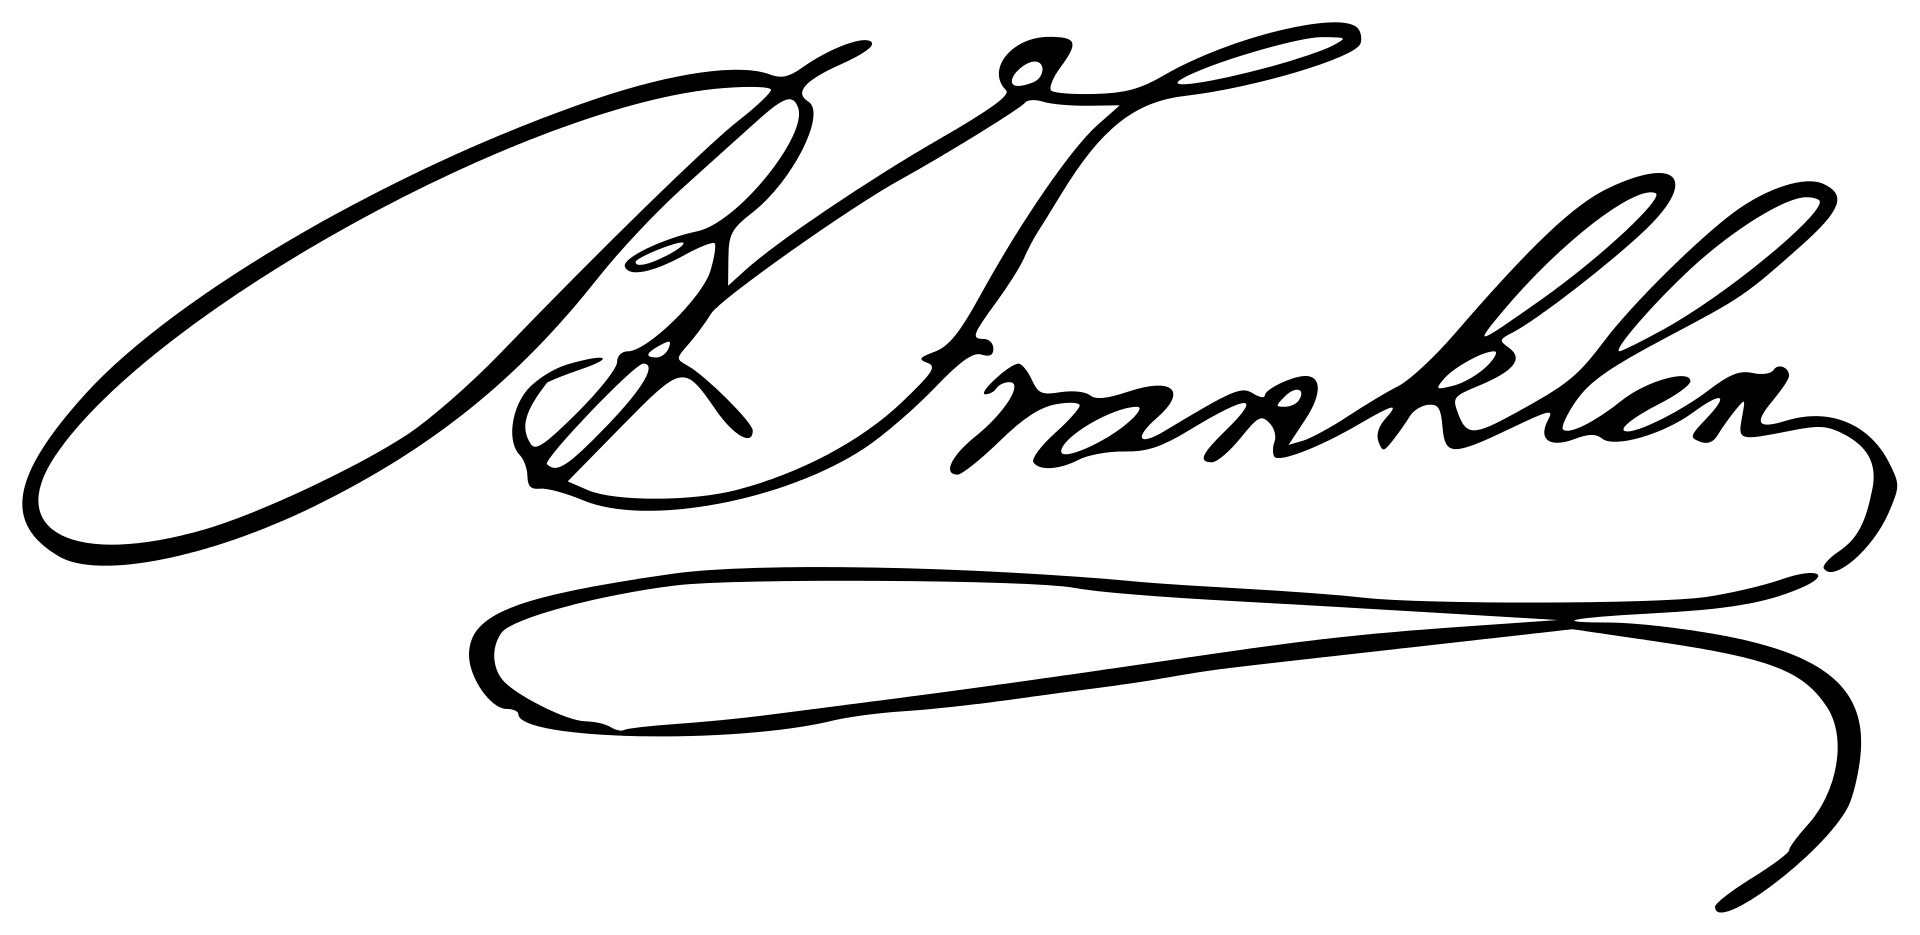
\includegraphics[height=1.5cm]{benjamin_franklin_signature} \\
%    \vspace{1cm}
    {Studentenommer / \textit{Student number}} & {Handtekening / \textit{Signature}} \\
    \hline
    & \\[-10pt]
    \textbf{L.\ Skywalker} & \textbf{1 October 2099} \\
    {Voorletters en van / \textit{Initials and surname}} & {Datum / \textit{Date}} \\
    \hline
\end{tabularx}

\vspace{15pt}


\chapter*{Abstract}
\addcontentsline{toc}{chapter}{Abstract}
\makeatletter\@mkboth{}{Abstract}\makeatother

The English abstract.



\selectlanguage{afrikaans}
\chapter*{Uittreksel}
\addcontentsline{toc}{chapter}{Opsomming}
\makeatletter\@mkboth{}{Opsomming}\makeatother

Die Afrikaanse uittreksel.

\selectlanguage{english}

\tableofcontents
%\listoffigures
%\listoftables
\chapter*{Nomenclature\markboth{}{Nomenclature}}
\addcontentsline{toc}{chapter}{Nomenclature}

% \vspace*{-3mm}
\subsubsection*{Variables and functions}

\begingroup
\renewcommand{\arraystretch}{1.2}
\renewcommand{\tabularxcolumn}[1]{p{#1}}
\begin{tabularx}{\textwidth}{@{}p{2.5cm}L}
    $p(x)$ & Probability density function with respect to variable $x$.\\
    $P(A)$ & Probability of event $A$ occurring.\\
    $\varepsilon$ & The Bayes error. \\
    $\varepsilon_u$ & The Bhattacharyya bound. \\
    $B$ & The Bhattacharyya distance. \\
    $s$ & An HMM state.  A subscript is used to refer to a particular state, e.g.\ $s_i$ refers to the $i^{\text{th}}$ state of an HMM. \\
    $\mathbf{S}$ & A set of HMM states. \\
    $\mathbf{F}$ & A set of frames. \\
    $\mathbf{o}_f$ & Observation (feature) vector associated with frame $f$. \\
    $\gamma_s(\mathbf{o}_f)$ & A posteriori probability of the observation vector $\mathbf{o}_f$ being generated by HMM state $s$. \\
    $\mu$ & Statistical mean vector. \\
    $\Sigma$ & Statistical covariance matrix. \\
    $L(\mathbf{S})$ & Log likelihood of the set of HMM states $\mathbf{S}$ generating the training set observation vectors assigned to the states in that set. \\
    $\mathcal{N}(\mathbf{x} | \mu, \Sigma)$ & Multivariate Gaussian PDF with mean $\mu$ and covariance matrix $\Sigma$.\\
    $a_{ij}$ & The probability of a transition from HMM state $s_i$ to state $s_j$. \\
    $N$ & Total number of frames or number of tokens, depending on the context. \\
    $D$ & Number of deletion errors. \\
    $I$ & Number of insertion errors. \\
    $S$ & Number of substitution errors. \\
\end{tabularx}
\endgroup


\newpage
\subsubsection*{Acronyms and abbreviations}

\begingroup
\renewcommand{\arraystretch}{1.2}
\begin{tabular}{@{}p{2.5cm} l}
    AE      & Afrikaans English \\
    AID     & accent identification \\
    IAT		& Improved automatic thresholding \\
    SNR		& Signal-to-noise ratio	\\
    PSNR	& Peak signal-to-noise ratio \\
    SSIM	& Structural similarity index measure \\
    NA		& Numerical aperture	\\
    PSF		& Point spread function	\\
    RACC	& Regression adjusted colocalisation colour mapping	\\
    DMEM	& Dulbecco's Modified Eagle Medium \\ %This is for treatments
    IHH		& Iterative hysteresis histogram	\\
    MIP		& Maximum intensity projection		\\
    RGB		& Red, green and blue
    
\end{tabular}
\endgroup

\newpage
\pagenumbering{arabic}

% Contents
\chapter{Introduction}
\label{chp:Intro}

%%%%%%%%%%%%%%%%%%%%%%%%%%%%%%%%%%%%%%%%%%%%%%%%%%%%%%%%%%%%%%%%%%%%%%%

%Add in a story regarding the change from colocalization to thresholding
\section{Background}\label{sec:background}
\subsection{Motivation for mitophagy research}
The human body is a multicellular organism comprised of many different organs and tissues, each of which is composed of an immense number of different types of specialised cells working together to enable the biological functions that allow us to live and act. The vast majority of these cells contain a number of specialised components fulfilling a number of functions and important among them is the mitochondria. The mitochondrion is an organelle that has developed to efficiently process food molecules, absorbed by the body, and convert them into a form of chemical energy that is easily used by the other organelles within the cell. This is crucial as cells with specialised functions in turn have specialised organelles to achieve them and typically the energy requirement is relatively high. Due to chemical wear and tear from performing their functions, or due to external forces, the efficiency and health of mitochondria can diminish and at their worst can become a hindrance to the healthy supply of energy for the cell.\par When this occurs a process called mitophagy activates where the irreparably damaged mitochondria are flagged, isolated, and broken down for the biomolecules composing it to be reused by the cell~\cite{cell_phys_book}. There are two organelles involved in this process and they are the autophagosome, involved with isolating and transporting the flagged mitochondria, and the lysosome, triggering the decomposition process which breaks down the mitochondria. There is a risk though of this mitophagy not activating correctly, or being dysfunctional, and is associated with a number of human illnesses particularly those that are neurodegenerative such as Alzheimer's disease and Parkinson's disease~\cite{mito_diseases}. It is for this reason that research into the mechanisms behind mitophagy, the causes of the dysfunction, and the correction of it is of value.

\subsection{The investigation of mitophagy}
The investigation behind the causes of dysfunction in mitophagy, and methods by which to correct it, can be approached in a number of ways. For studying the regulation and correction of mitophagy dysfunction it is more accessible to observe the behaviours of the mitophagy-relevant organelles using cell cultures. These observations can be performed either visually, chemically, or both to determine which organelle behaviours are associated with functional or dysfunctional mitophagy. To achieve this, a common approach is to apply treatments that target specific factors (chemical, thermal, physical, etc.) that stress the mitochondria. Once the mitochondria are sufficiently stressed, mitophagy will be triggered allowing us to observe the actions of the mitochondria and involved organelles (autophagosomes and lysosomes). Treatments can target different factors to measure their influence in triggering mitophagy or can induce dysfunction in mitophagy. Visual observation of these events provides greater spatial information with regard to the organelles (position, size, count) especially with many interactions being spatial (engulfment, joining, separation, etc.) and is achieved through microscopy imaging.

\subsection{Preparation of images prior to analysis}\label{sec:intro_noise}
The purpose of imaging is to capture a representation of the specimen that can be measured by visual and image analysis with the former being performed by humans with qualitative (e.g. estimating the shape of the subjects in the image) or quantitative (e.g. manually counting each individual subject) measures while the latter is performed by machines through algorithms that are able to provide more detailed quantitative measurements (e.g. the calculated distribution of subject sizes within a population which provides measures such as the mean or variance of the sizes). An obstacle to the accuracy of both the visual and image analysis is image degradation which is the loss of image quality due to the presence of a number of factors in the image. There are a number of different factors causing this image degradation but the three most prominent are noise, distortion and artefacts. Noise typically causes a misrepresentation of the intensities within an image and generally acts as an additive component~\cite{digitize_noise_chapt}. Distortion is a deformation in the spatial representation of the specimen being imaged with the shape and position of structures primarily being affected. Artefacts are a broad group that refers to any anomalous elements in the image that do not fall under the prior factors and could affect the intensity or spatial representations of the specimen. A common attribute among these is that they are undesired in the image and either obscure the structures of interest, misrepresent their features (e.g. size, shape, texture, etc.); or describe non-existent, or unintended, structures. If this image degradation remains then analysis of the image is less reliable with the results being skewed depending on the degradation factors present. Unfortunately, there is always some degradation present in all images but the impact depends on both the quantity of these factors and the sensitivity of the features that are being analyzed (e.g. structures or structural features that are small or fine in size are usually more sensitive).\paragraph{Restoring image quality:} The restoration of image quality and clarity has motivated the development of a number of techniques over many years. These techniques typically aim to reduce the impact of the aforementioned factors such that the image becomes a closer representation of the specimen improving the accuracy and reliability of further analyses. These techniques have typically been developed to target specific factor(s) (e.g. removing specific types of noise or distortion specifically) with each having optimal conditions (e.g. consistent illumination, high contrast between foreground and background, etc.) to perform effectively and when these conditions are not met the outcomes can be unsatisfactory for any analysis. It is for this reason that the applied techniques need to be correctly chosen based on the factors present within the image. These techniques can be roughly grouped together based on their intended outcome whether it be deconvolution techniques reducing the distortion caused by microscope diffraction; denoising techniques which reduce the presence of noise; image enhancement techniques which emphasise or correct image properties such as improving contrast or smoothing unequal illumination across the image; and binarizing techniques which segment structures between the foreground and background with the foreground typically being what is of interest to analysis. These are merely categories and based on the criteria and desired granularity sub-groups can be made such as ``wavelet filters'' and ``patch-based filters'' which may still share overlapping outcomes. 
\paragraph{Binarizing techniques:} 
These techniques focus on the separation of pixels between a foreground and background resulting in a binary image. The application of this can be quite broad but for the purposes of this research, the binary separation of pixels allows clear differentiation between what is and is not of interest to succeeding analyses. A commonly employed set of techniques in image analysis, to achieve binarization, are thresholding techniques where numeric threshold(s) are calculated from the image and used to determine whether a pixel belongs to the foreground or background based on whether the pixel intensity is greater than the threshold or not, respectively~\cite{segmentation_book}.
Effective binarization enables the selectivity of structures that can be of particularly great benefit to any image analyses employing quantitative measurements that are highly sensitive to the image quality (e.g. Gaussian noise can greatly compromise structure count measurements). Through this, the measurements taken can be isolated to only the foreground structures where the degradation factors may be weaker.
\paragraph{Thresholding groups:}
As mentioned previously, thresholding is a common method of \\achieving binarization but typically falls into two groups for image processing. These are global thresholding and local thresholding methods with each having their own respective pros and cons.
\begin{multicols}{2}
\textbf{Global methods}
\begin{itemize}
    \item Relies on the image histogram to determine the threshold value.
    \item Applies this threshold to all image pixels naively.
    \item Sensitive to both distortions of the image histogram and localised variations in image intensity.
    \item Require few, if any, parameters for optimal performance.
\end{itemize}
\columnbreak
\textbf{Local methods}
\begin{itemize}
    \item Determines the threshold of each pixel by evaluating the intensity characteristics of the localised region centred on it.
    \item Robust to localised characteristics in images (e.g. variations in contrast around structures).
    \item Performance is dependent on one or more parameters that may need to be tuned for each image for optimal results.
\end{itemize}
\end{multicols}
Despite this, both methods can still be sensitive to other degradation factors present in the image regardless of whether a global or local method is used.

\subsection{High-throughput pre-processing}
High-throughput pre-processing is where the pre-processing of images is optimised for both speed and the resultant image quality. This is usually applied to large batches of images and can form part of a larger high-throughput analysis sequence with the goal of expediting image analysis while maintaining accuracy. To optimize the improvements to the image quality achieved by the pre-processing it is not uncommon to sequentially apply pre-processing techniques to images in a pipeline. This acts as a synergistic process where the outcomes of preceding techniques in the pipeline can optimize the conditions for succeeding techniques allowing them to produce higher quality outcomes than if they were applied in isolation. A key component of high-throughput analysis is speed which is achieved by minimizing interruptions in the pre-processing by using automated techniques that do not require parameters to be tuned to achieve adequate results. 


\section{Problem Statement}\label{sec:problem_state}
After imaging a large number of various cells, all under identical imaging conditions (e.g. resolution, brightness, gain, etc.), it is often the case that high-throughput pre-processing be implemented as part of preparing them for analysis.  This approach ideally enables efficient and effective pre-processing, thereby saving time for studies and projects dealing with extensive batches of images. However, the involvement of binarization in this process can pose a challenge to the goals of high-throughput pre-processing. \par Binarization is challenging in high-throughput pre-processing due to the constraints that automatic global and local thresholding methods can impose. Global thresholding has a high sensitivity to intensity-related factors (e.g. noise) and image properties, such as contrast or brightness, that affect the histogram particularly when these vary over localised regions of the image. This can result in inconsistent results that can vary greatly based on each image. Local thresholding is more robust to localised variations across the image and is unaffected by the histogram but the quality of the results is dependent on the parameter tuning. Parameter tuning is a human-involved process of adjusting parameter values to attain the most accurate thresholding results but can be time-consuming to perform and the degree of tuning necessary can be worsened by the presence of degradation factors. This results in a situation where global thresholds provide simplicity of application but uncertainty in behaviour while local thresholding can provide robust results given that the parameters are sufficiently tuned for each image, disrupting the pacing of the high-throughput pre-processing.\par This is not a constant where pre-selected parameter values may be sufficient for a local threshold technique or the intensity-related image properties are consistent enough that there is minimal variation for global thresholding techniques. Resolving this problem through a solution that provides both the robustness of local thresholds with the simplicity of global thresholds would provide more opportunities for studies requiring the pre-processing of large image batches to expedite this research and save time. Providing an effective binarization solution could reduce the outcome of poor binarization which ranges from the inclusion of noise as structures of interest for analysis or the exclusion of structures important to the study. While machine learning solutions to similar problems exist~\cite{machine_segment}, their performance can be dependent on both the type and quantity of data they are trained on but this training data can be expensive or time-consuming to acquire.

\section{Project objectives}\label{sec:objectives}
To resolve this problem of binarization in high-throughput pre-processing a system will be designed based on these objectives:
\begin{enumerate}
    \item Optimize the binarization outcomes without parameter tuning being required.
    \item Be an automated method that can be integrated into a high-throughput pipeline.
    \item Most provide results similar to or exceeding established methods such as global or thresholding methods in a high-throughput context (no parameter tuning).
\end{enumerate}
These objectives will guide the design of a deterministic binarization system which will be referred to as Improved Automatic Threshold (IAT).

\section{Scope}
The constraints on the expectations for the development and evaluation of this binarization solution are:
\begin{enumerate}
    \item Commonly extracted structure features of the image that can be quantified by existing libraries (e.g. scikit-image~\cite{scikit-image}, SciPy~\cite{scipy}, etc.)  will be used to determine the binarization. Structure count, structure volumes, intensity distribution across structures, and structure-specific intensities. Combinations and transformations (e.g. averages, derivatives, etc.) of these features will also be considered.
    \item The system will be agnostic to image resolution and freely be able to process 2D and 3D images.
    \item The developed method will be evaluated against existing automatic global and local thresholding methods both quantitatively, using metrics such as signal-to-noise ratio (SNR), and qualitatively. The qualitative evaluations will entail visual analysis of the thresholding outcomes and will also be compared to manually thresholded images but not as extensively as the quantitative evaluation due to time constraints.
    \item This research is pursued application to imaging relevant to the study of mitophagy thus only the imaged mitochondria, autophagosomes, and lysosomes will be used for development and evaluation.
    \item Only images for a single type of microscopy will be used for both the development and evaluation of this method due to both time and resource constraints.
\end{enumerate}

%The Memantine research investigated the impact of Memantine, a medication, on the mitophagy process with a particular focus on the relationship between its influence on mitophagy relative to the concentration of the medication. There were multiple data sets collected that were acquired through fluorescence microscopy imaging to provide further data for both supporting more reliable conclusions from the data and to compensate for challenges in the data collection. It was found that there were challenges in the data collection were images with too much noise, weak fluorescence signals from objects of interest and non-specific fluorescent probes (staining more than the intended objects e.g. a mitochondria stain also staining the cytosol of the cell) increased the difficulty of forming accurate analysis and observations of those samples thus more was required. 


\section{Contributions}
Contributions made through this research were to the paper \textit{The Highs and Lows of Memantine—An Autophagy and Mitophagy Inducing Agent That Protects Mitochondria}~\cite{sholto_research} by assisting in sample pre-processing and image quality evaluation prior to analysis. Further contributions that are discussed are the potential contributions that this research could provide towards the image analysis, and related, fields.
\subsection{Contributions towards the Memantine research paper}
The IAT developed in this project originated from the application in high-throughput pre-processing of mitophagy-related organelle images to expedite data set preparation for mitophagy analysis. Coincidentally, research regarding the application of Memantine treatments and the analysis of its effects on mitophagy behaviour~\cite{sholto_research} was pursued. Despite the IAT project shifting focus from mitophagy analysis to image pre-processing, with a focus on mitophagy-related organelle images, support was provided to the Memantine research with regard to the image pre-processing and the evaluation of the image quality prior to mitophagy analysis. 

\paragraph{First contribution:} 
The development of a pre-processing pipeline macro for FiJi~\cite{Fiji_paper} to automate the pre-processing of 3D confocal fluorescence microscopy images of cellular organelles which are mitochondria, lysosomes, and autophagosomes. The pipeline used was based off of the pipeline described in \cite{PipelineDecon-Chaudhry} (excluding the binarization and all succeeding algorithms) with adjustments made detailed in Section \ref{sec:preprocess_applied}.

\paragraph{Second contribution:} 
With pre-processing having been applied, the quality of these images were evaluated under three criteria:
\begin{enumerate}
	\item Sufficient contrast of the structures of interest against the background, and any residual noise, for accurate differentiation.
	\item The lack of fluorescence falsely describing in-focus structures originating from either out-of-focus fluorophores, fluorescence cross-talk, and autofluorescence.
	\item Confident clustering of organelles in the images between separate cells if present.
\end{enumerate}
The first criterion being met implies that structures of interest can be differentiated and selected for algorithmic analyses where those results could be disturbed by erroneously including noise. The second criterion being met implies that aberrations in the image that are more challenging to automatically remove, without degrading the image signal, are not strongly present and will not distort measured results. The final criterion being met implies that per cell measurements are possible to capture for an image which is necessary for certain analyses.

\subsection{Contributions towards relevant fields}
The fields of relevance to this research are image analysis, with the focus on image binarization, and cellular physiology, as the data used in throughout the IAT development involved cellular organelle images. This will provide a binarization solution accessible to those with low expertise in image pre-processing while providing viable results particularly for high-throughput applications. For image analysis, the contribution will be the establishment of a new automated thresholding method with a novel approach to approximating binarized images. 

\section{Structure of thesis}
This thesis is composed of 6, including Chapter 1, with the remaining 5 Chapters summarised below:\par
\textbf{Chapter \ref{chp:Background}} provides context around many facets of this research project to build a fundamental understanding of certain decisions in the system design and the phenomena that are observed. These fundamentals are composed of context for the organelles being imaged in regard to their characteristics; the microscopy techniques used and how they function; a high-level overview of the pre-processing method groups and the roles each play in improving image quality; and specific methods that are of note to the system design.\par
\textbf{Chapter \ref{ch:methodology}} will present the rationale behind the preparation of the specimen which is imaged, the pre-processing techniques applied to improve the image quality, and the design of the system IAT to binarize the objects of interest with observations and tests to justify said design choices.\par
\textbf{Chapter \ref{ch:results}} will present and discuss the performance results of the IAT against established thresholding methods.\par
\textbf{Chapter \ref{ch:conclude}} will provide a conclusion regarding the performance of the IAT method, the shortcomings, and improvements to be made through future work.  

\begin{figure}[h!]
    \centering
    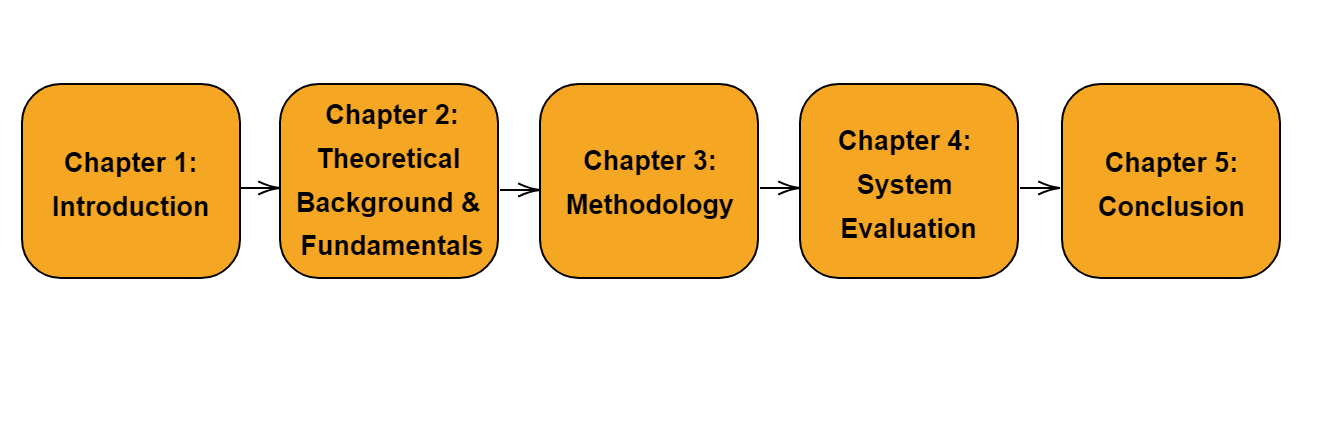
\includegraphics[width=\linewidth]{figs/thesis_structure_diagram.png}
    \caption{Diagram of thesis structure}
    \label{fig:thesis_struct_diag}
\end{figure}
 
\chapter{Theoretical Background \& Fundamentals}
\label{chp:Background}
% \section{Relation to Chapter \ref{chp:Intro}}
In Chapter \ref{chp:Intro} the research regarding mitophagy is mentioned and the research to develop automated thresholding methods to streamline the data preparation process is detailed in terms of objectives and the proposed use case. Before detailing related research or the design of the proposed thresholding system an initial establishment of theoretical information regarding the mitophagy research use case will be presented. This theoretical information will regard the organelles being imaged for mitophagy analysis, the mitophagy process itself, the microscopy techniques employed for imaging, an overview of image preprocessing techniques that may be employed (noise removal, deconvolution, thresholding) and other particular techniques of interest to the thresholding system design.

\section{Mitophagy and involved organelles}\label{sec:mito_detail}
%In Section \ref{sec:background} the motivations for researching the Mitophagy process are raised including the stipulation of the organelles of interest for this Mitophagy research. To briefly reiterate these points, mitophagy as a process involves the recycling of overly damaged mitochondria to maintain mitochondrial health in cells where dysfunctional mitophagy has been observed in a number of illnesses. For the purpose of this proposed Mitophagy research, the cellular organelles involved with the mitophagy process that is being imagined will be discussed further in function and structure.
In Section \ref{sec:background} a number of potential applications of mitophagy research were presented. Of importance were the overview of the organelles involved in mitophagy, the purpose of these organelles and the importance of mitophagy with regard to these organelles. As these organelles and the mitophagy process will studied via visual and image analysis the function but also the structure will be discussed further in this section.
\subsection{Mitochondria}\label{sec:mitochondria}
Mitochondria are organelles found in plants, animals and many other multicellular organisms that are primarily responsible for supplying the energy required by the cell. The primary functions and mitochondria structure will be discussed in this section.
\subsubsection*{Functions}
The mitochondria perform a number of functions within the cell but the most notable function is the provision of fuel for the cell for the other contained organelles to play their role in maintaining the cell and executing their actions relative to the rest of the cells. This fuel is synthesized by the mitochondria in a molecule called adenosine triphosphate (ATP) which is an efficient fuel format accepted by all other energy-consuming organelles within the cell. This is crucial to the survival of cells as the many chemical and mechanical actions performed by cells can be energy expensive and the extraction of energy from food energy molecules is of a low yield with much of the desired energy remaining chemically trapped~\cite[p. 33, 35, 40]{cell_phys_book}. For this reason, mitochondria are dedicated to producing ATP which effectively yields energy when required and the number of mitochondria in cells ranges from hundreds to thousands depending on the cell functions. This is not the sole function of mitochondria as they are instrumental in the management of controlled cell death (apoptosis) which is employed when the cell itself is too damaged for repair deeming it to be of risk to the surrounding cells~\cite[p. 40-41]{cell_phys_book}.
\subsubsection*{Structure}
The structure of mitochondria is that of an oval-like structure with many cristae (internal folds) increasing the internal surface area and improving the efficiency of ATP synthesis process. A visualisation of this internal structure can be seen in Figure \ref{subfig:mito_folds} and these mitochondria coexist separately from each other in the cell in a formation called `punctate' or they can appear in a formation called a `reticulum'. A mitochondrial reticulum (shown in Figure \ref{subfig:mito_retic} is formed primarily in cells with a higher energy demand than usual such as skeletal muscle and this reticulum is akin to a connected branching structure. This branching allows mitochondria to support each other by sharing functional components as ATP production can cause wear to build up as a byproduct.
\begin{figure}
    \centering
    \subcaptionbox{Image of an individual mitochondria\label{subfig:mito_folds}}{\stackinset{r}{}{t}{}{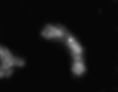
\includegraphics[width=0.1\linewidth, cframe=orange 1pt]{figs/ch2figs/Crop_punctate.png}}{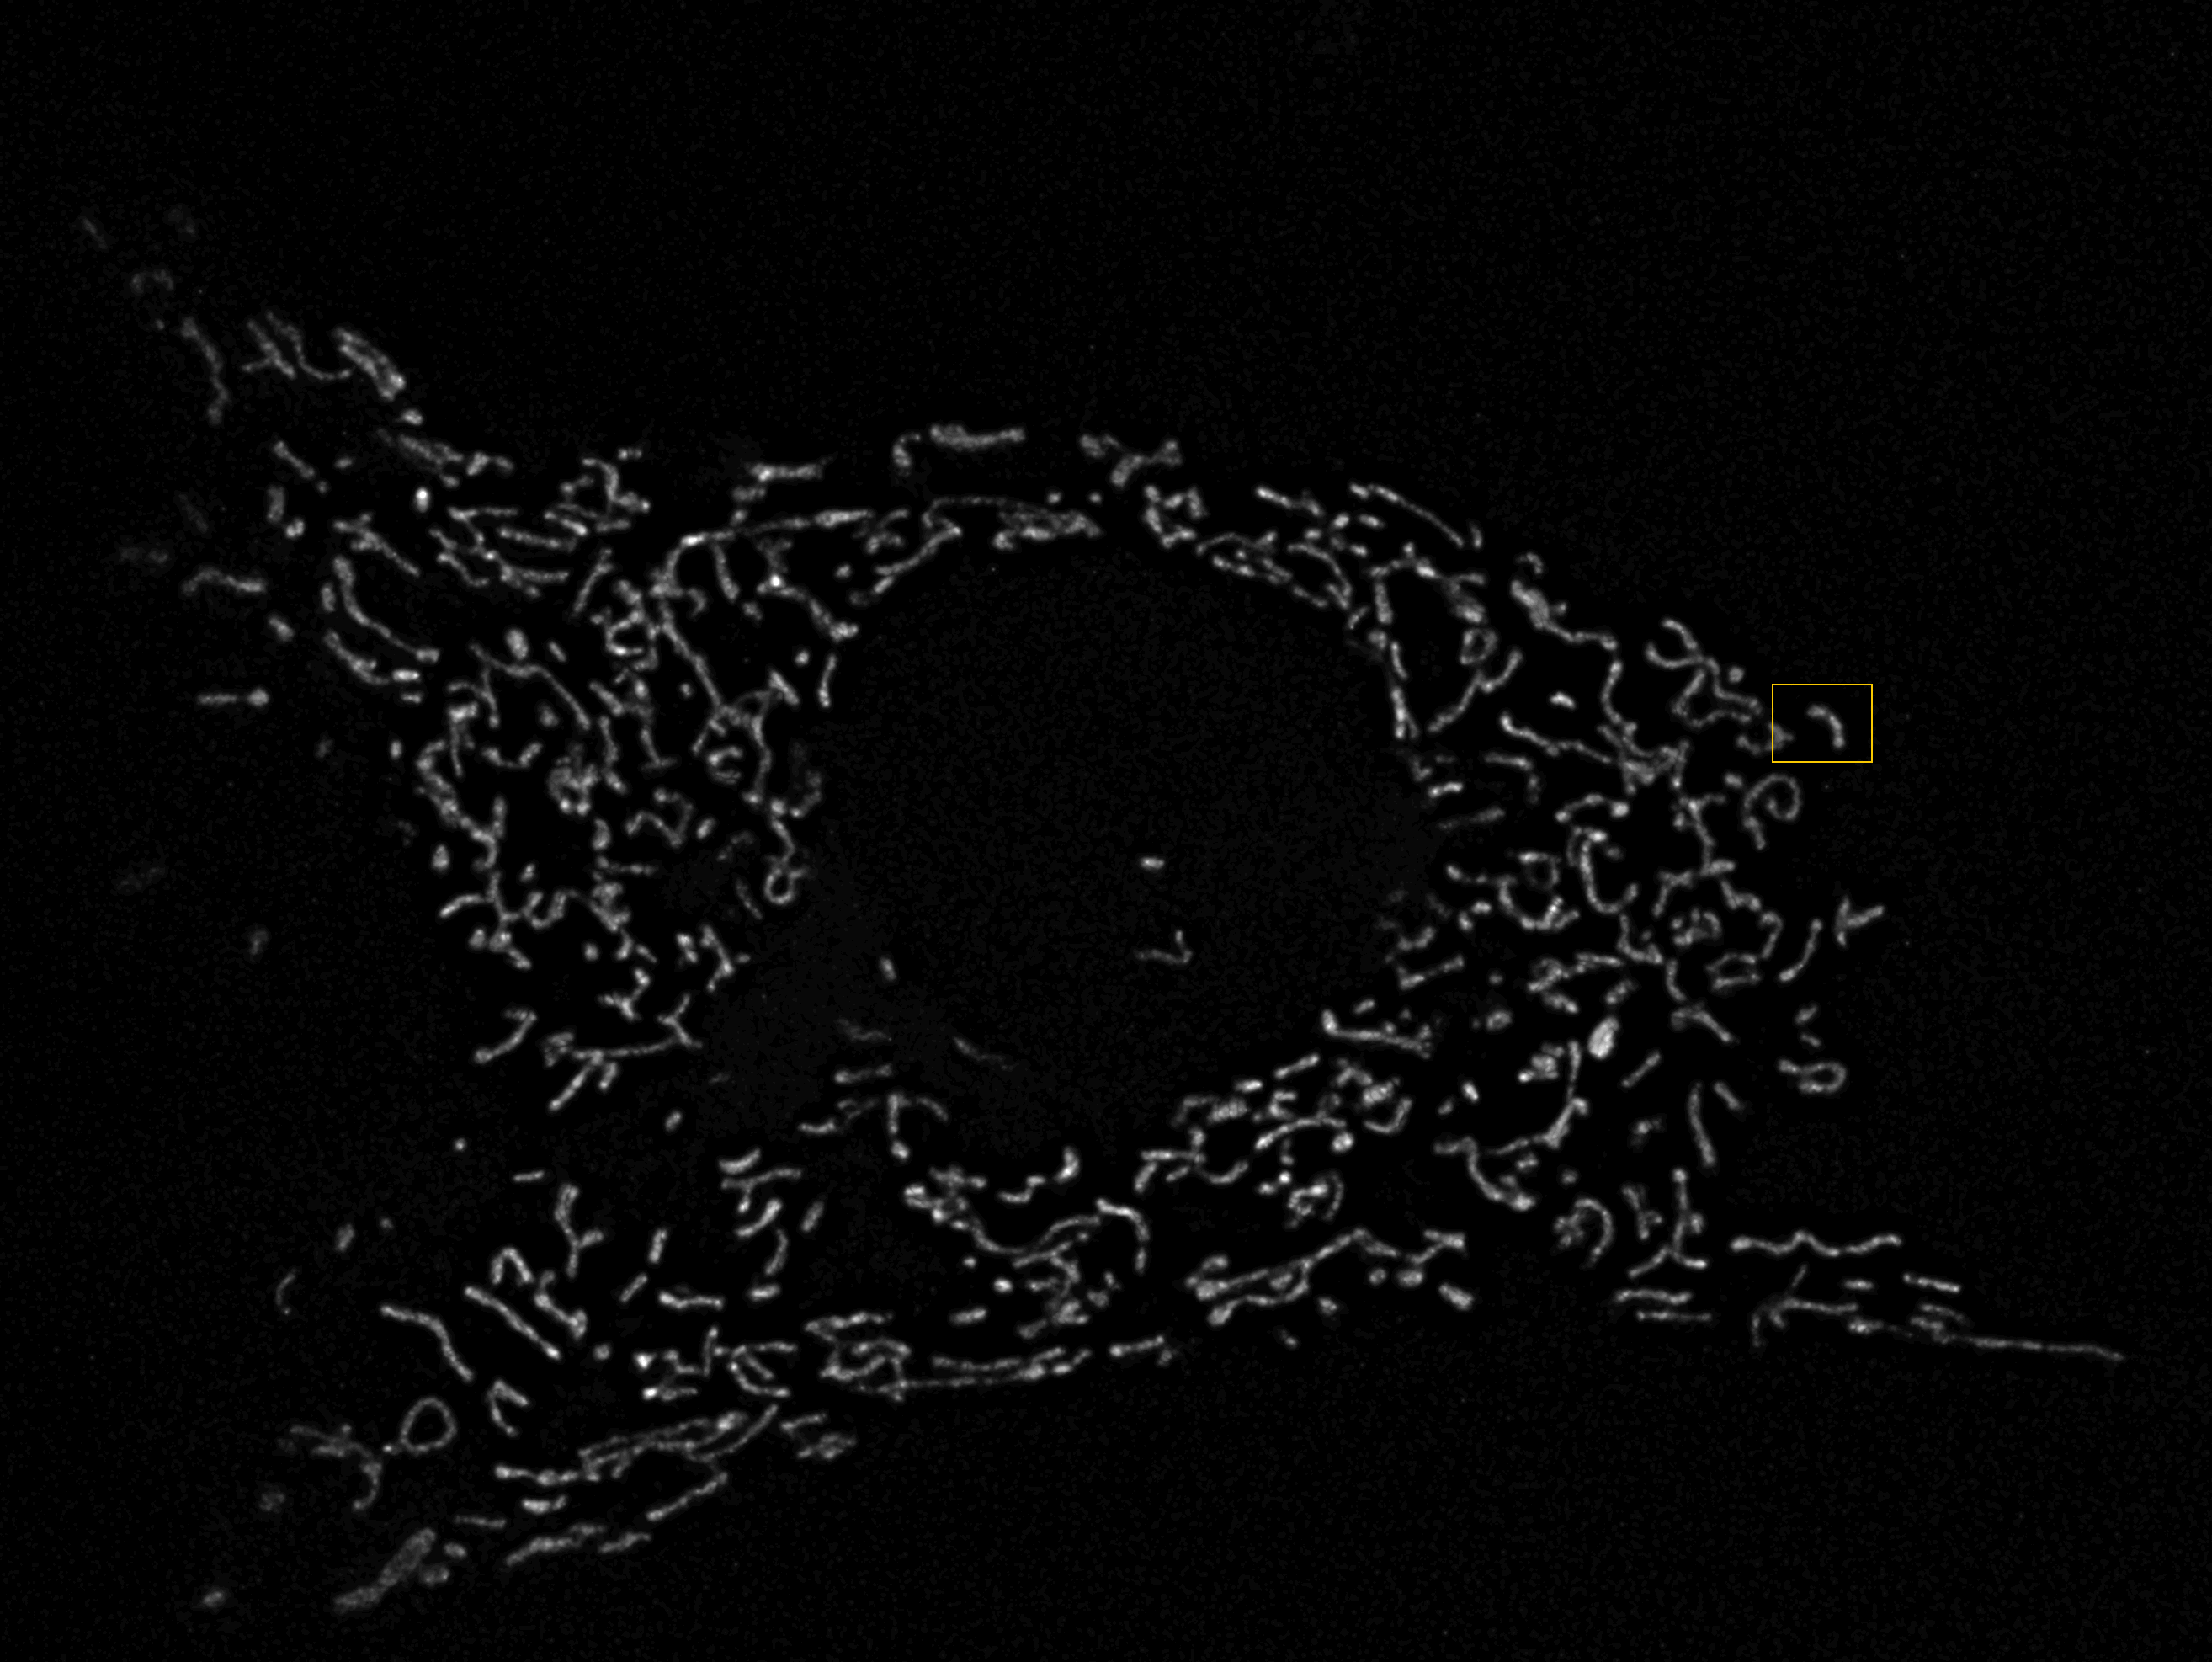
\includegraphics[width=0.49\linewidth]{figs/ch2figs/MAX_CCCP_1C=1T=0_punctate.png}}}
    \subcaptionbox{Image of the mitochondrial reticulum\label{subfig:mito_retic}}{\stackinset{r}{}{t}{}{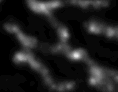
\includegraphics[width=0.1\linewidth, cframe=orange 1pt]{figs/ch2figs/Crop_branched.png}}{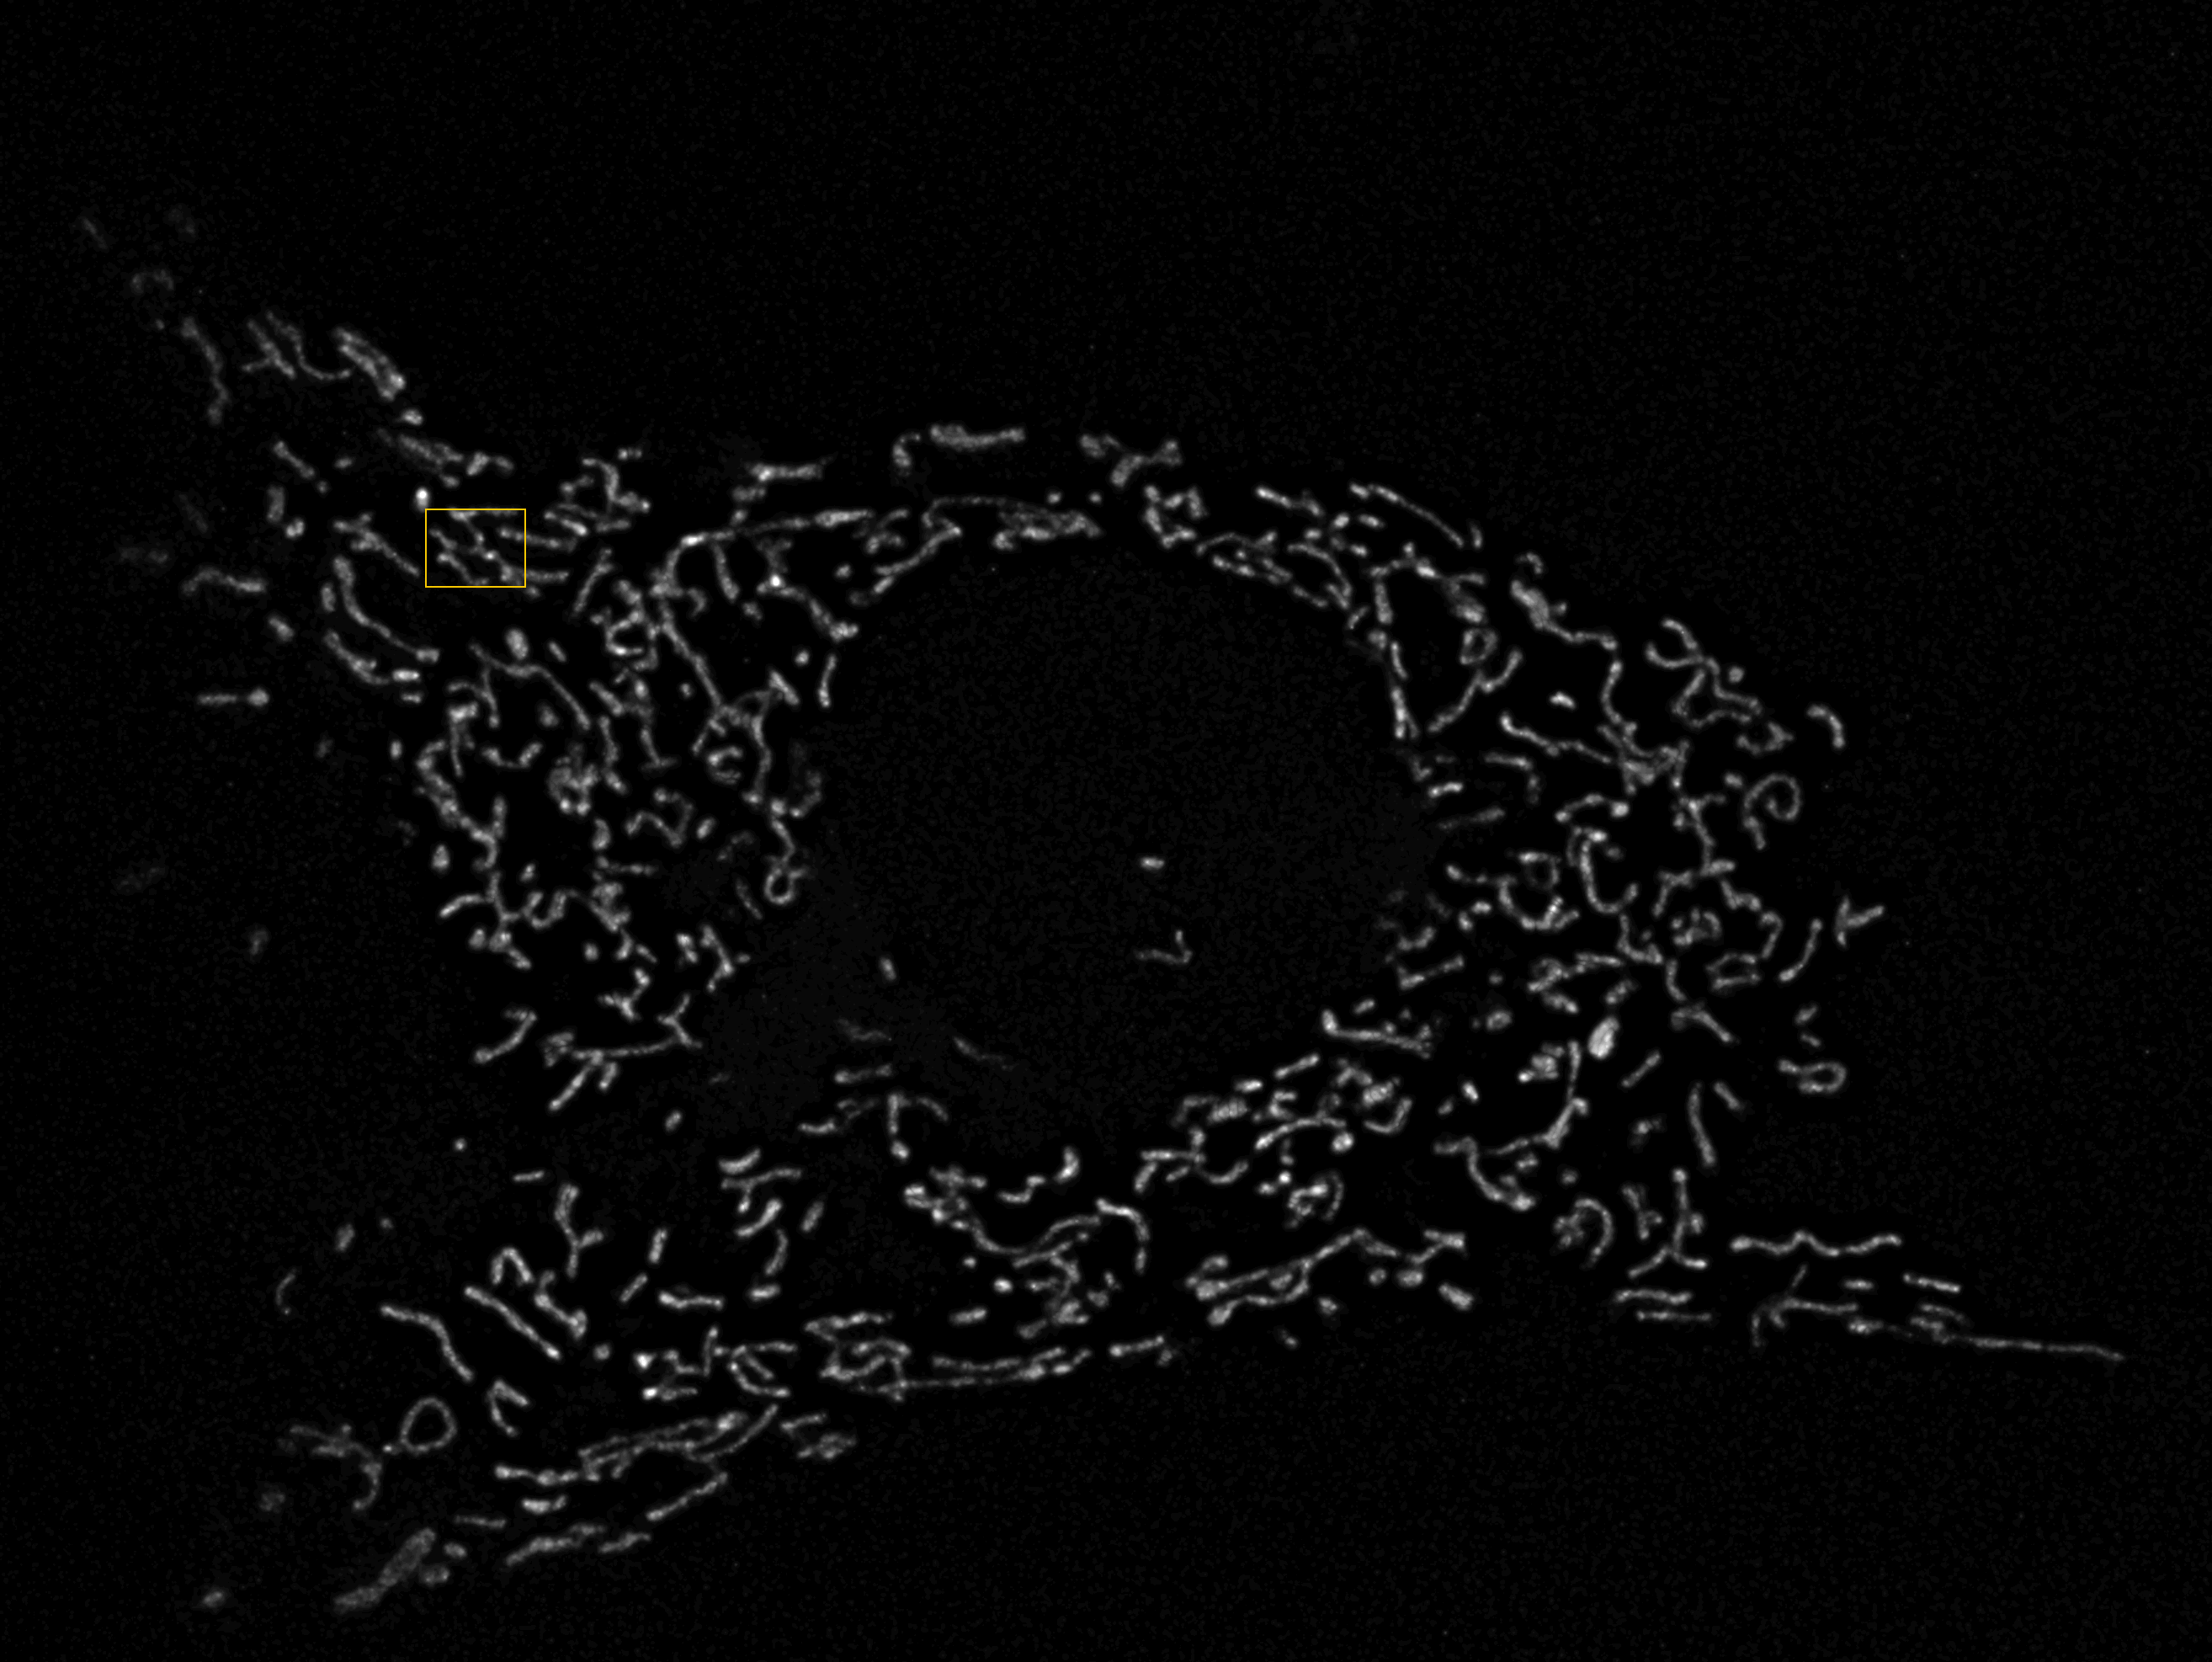
\includegraphics[width=0.49\linewidth]{figs/ch2figs/MAX_CCCP_1C=1T=0_branched.png}}}
    \caption[Comparison between punctate and branching mitochondria structures]{Comparison between mitochondria structure types with (\subref{subfig:mito_folds}) singular punctate mitochondria and (\subref{subfig:mito_retic}) branching mitochondria forming a reticulum}
    \label{fig:mito_struct}
\end{figure}
\subsection{Lysosomes}\label{subsec:lysosome}
Lysosomes are organelles involved with the recycling and degradation of compounds and organelles within the cell.
\subsubsection*{Function}
The purpose of lysosomes is to decompose compounds within the cell into the base components which can be used to synthesize new organelles or provide needed nutrients. The lysosome is a carrier of hydrolases (an enzyme that reacts with water to break down molecules) that break down specific compounds within the cell ranging from biomolecules absorbed from outside the cell such as proteins, carbohydrates and lipids; to invasive bacteria; and even damaged organelles. The breaking down of compounds absorbed from outside of the cell (through a process called endocytosis) is used to `digest' these compounds to provide a source of new nutrients. The decomposition of invasive bacteria and damaged organelles acts similarly to a defence response to maintain the health of the cell while also allowing the damaged organelles to be recycled to produce new organelles maintaining the population of healthy organelles~\cite{lyso_auto_relation, cell_phys_book}. The process of decomposing these compounds is called \textit{autophagy} and relies on autophagosomes to deliver the compounds, to be decomposed, to the lysosomes. The lysosome fuses with the autophagosome to become an \textit{autolysosome} where the contained compounds are introduced to hydrolase enzymes initiating decomposition~\cite{lyso_auto_relation}.
\subsubsection*{Structure}
Lysosomes are small structures of spherical bodies composed of a membrane-like structure containing the hydrolase enzymes~\cite{cell_phys_book}. This membrane structure is impermeable to most interfacing to prevent the unintentional release of the contained enzymes~\cite{lyso_auto_relation}.

\subsection{Autophagosomes}\label{subsec:autophagosome}
Autophagosomes are the name for the membrane structure that carries compounds to be decomposed by autophagy.
\subsubsection*{Function}
Autophagosomes are formed from phagophores (a cup-shaped membrane) that are located in the cytosol (cellular fluid) and stretch to engulf the compounds to be decomposed. Once the compounds have been engulfed the phagophore is referred to as an autophagosome which proceeds to carry the contents to a lysosome. An autophagosome is one of the organelles capable of interfacing with lysosomes to form an autolysosome. After fusing together the lysosome introduces the enzymes to the cargo of the autolysosome and autophagy begins~\cite{lyso_auto_relation}.
\subsubsection*{Structure}
An autophagosome is initially a single membrane called a phagophore which stretches and deforms into a cup-like shape when approaching biomolecules that are supposed to undergo autophagy. The phagophore continues to stretch around the biomolecules until they are fully engulfed at which point the edges of the cup-like shape join and fuse to form a double membrane. The phagophore is now referred to as an autophagosome with a complete double membrane which has an ovular/spherical shape.

\subsection{Mitophagy}
With the relevant organelles, and their functions, briefly covered a simple description of the mitophagy process can be presented. As mentioned in Section \ref{sec:background}, the dysfunction of mitophagy is associated with a number of diseases with neurodegenerative disorders (e.g. Parkinson's disease, Alzheimer's disease, etc.) of note. Mitophagy as a process refers to the isolation and subsequent decomposition of dysfunctional mitochondria. This is performed by the autophagosomes engulfing the mitochondria and transporting them to lysosomes as cargo. The autophagosomes fuse with the lysosomes introducing enzymes to the mitochondria and beginning the decomposition process. After the decomposition is completed the resultant molecular components of the mitochondria can be used by the cell in a number of ways such as synthesising new mitochondria.\par The reasons why mitochondria are degraded by autophagy is typically due to irreparable mitochondria dysfunction usually caused by either physical, chemical or oxidative damage. This damage to the mitochondria can affect a number of components (mitochondrial DNA, lipids, proteins, etc.) that are necessary for many mitochondrial functions and while this damage is below a certain threshold the impact of this damage on mitochondrial functions can be mitigated through fusion. This fusion entails the joining of mitochondria to share functional components to compensate for those that are damaged allowing mitochondrial functions, like ATP synthesis, to continue~\cite{MitoFus-2012}. Multiple fusions can occur between mitochondria allowing branching chains of mitochondria to form, mentioned in Section \ref{sec:mitochondria} as a mitochondrial reticulum, which is more frequently seen in cells undergoing high ATP demand such as activated skeletal muscle cells~\cite{cell_phys_book}. This makes the network of fused mitochondria robust to interference in ATP production when there are high energy demands.\par 
Previously it was mentioned that fusion could compensate for damage to the mitochondria given that the damage is below a threshold but what happens when this threshold is exceeded? When this occurs the mitochondria can be seen as irreparable and if present in a reticulum then the density of dysfunctional components could place undue strain on the fused mitochondrial collective. The first step in this process is mitochondrial fission where dysfunctional components are aggregated to a singular region within the mitochondria which are then split into two daughter mitochondria. The daughter mitochondria containing dysfunctional components can then be removed via autophagy while the healthy daughter can resume activities. In the case of a fused mitochondria network, this aggregation still occurs and only the localised region containing the dysfunctional components will be split from the network~\cite{MitoFus-2012}.\par With the dysfunctional mitochondria separated from the healthy a number of mitochondria-specific biochemical pathways (mechanisms), which will not be described further here, activate flagging the dysfunctional mitochondria. With the dysfunctional mitochondria flagged and located the phagophores can engulf the mitochondria, becoming an autophagosome, and transport it to a lysosome to begin decomposition~\cite{MitoMechan, MitoFus-2012} (described in Sections \ref{subsec:lysosome} and \ref{subsec:autophagosome}).

\section{Fluorescence Microscopy} \label{sec:fluorMicr}
%For cluster tracking and detection for cells: https://link.springer.com/article/10.1007/s40846-016-0216-y
As described in Section \ref{sec:background}, a particular method of studying mitophagy behaviours is to study the organelles involved in this process (detailed prior in Section \ref{sec:mito_detail}). There are a number of methods by which to analyse organelle behaviours whether visual or biochemical where each captures different ranges of traits describing these behaviours. For the study of mitophagy, it is not uncommon to employ a combination of visual and biochemical analysis but it is the visual analysis that is of interest to this particular research. This section will explore the high-level motivation behind fluorescence microscopy as opposed to traditional optical microscopy, the factors to consider for suitable fluorophore selection, the limitations of fluorescence microscopy, an overview of confocal fluorescence microscopy, and a brief breakdown of the relevant microscopy apparatus.

\subsection{Light microscopy and motivations for fluorescence microscopy}\label{sec:lightVsFluoro}
In the microscopy of both cellular and subcellular structures, there are numerous biochemical structures, biomolecules and intracellular processes that can be observed. For this research, organelles are the subcellular structures that are of interest and going forwards will be referred to simply as `structures'. A traditional, and still used, method to visually observe these structures is through the use of optical microscopy. 
\paragraph{Optical microscopy} exposes the biological specimen, placed on the microscope stage, to visible spectrum light illuminating the specimen allowing cells, organelles, and other biochemical structures to be seen. When imaging these specimens there are three obstacles to making accurate and clear observations of the specimen, particularly with subcellular objects. These are the resolution limit where optical microscopes struggle to resolve features (edges, gaps between structures, etc.) that are smaller than $0.2\mu$m~\cite[p.582]{GeneralMicroscop}; thick specimens reduce the level of clear detail at higher resolutions; and that these specimens are frequently composed of majority water thus structures and features may be indistinct if not nearly invisible~\cite[p.585]{GeneralMicroscop}. The challenge of thick specimens can be resolved by slicing the specimen and improving the clarity due to the high water contents can be resolved through the use of stains which bind to cell structures, bacteria and other microscopic organisms based on the stain's preferred conditions. This allows stains to be selected that will localise to specific structures or to specific cellular processes (e.g. metabolic) improving the contrast between these structures from the irrelevant surroundings. Despite this, there can still be visual interference from surrounding structures which can decrease the clarity at which fine structures or features can be discerned.\par 
\textcolor{red}{For the above paragraph, and in future, I use the paragraph{} command to head off new points in the subsubsection that is contained within the paragraph. I realise now, after going through a few sections, that there are extra spaces after the bolded paragraph heading. Do you think this looks fine, should I linebreak after the paragraph heading, or do you think I should bold text the first word (as I have done now) but without the space after which will use textbf and linebreak to replicate the effect.}
\paragraph{Fluorescence microscopy} is similar to optical microscopy except for the types of stains utilised and some adjustments to the microscope architectures. Fluorescence microscopy utilises fluorescent stains, called fluorophores, that are identical to the stains described prior except that they emit light of a specific wavelength (based on the fluorophore) when excited. This excitation of the fluorophores is likewise induced by exposing these fluorophores to the light of a fluorophore-specific wavelength allowing the selection of which structures are visible by constraining both the wavelength of light illuminating the specimen and the wavelength that is captured by the microscope. This wavelength selection for both the excitation and emission light is achieved through filters that reject wavelengths outside of the currently selected range allowing structures to be indicated by specific wavelengths~\cite{Sanderson-2014}. For this reason, fluorescent stains can be referred to as indicators and fluorescently stained structures can be referred to as `indicated' where post-imaging different colours can be assigned to these respective wavelengths improving differentiation between different types of indicated structures. A comparison between optical and fluorescence microscopy can be seen in Figure \ref{fig:microscopeTypeCompare}.

\begin{figure}[h]
    \centering
    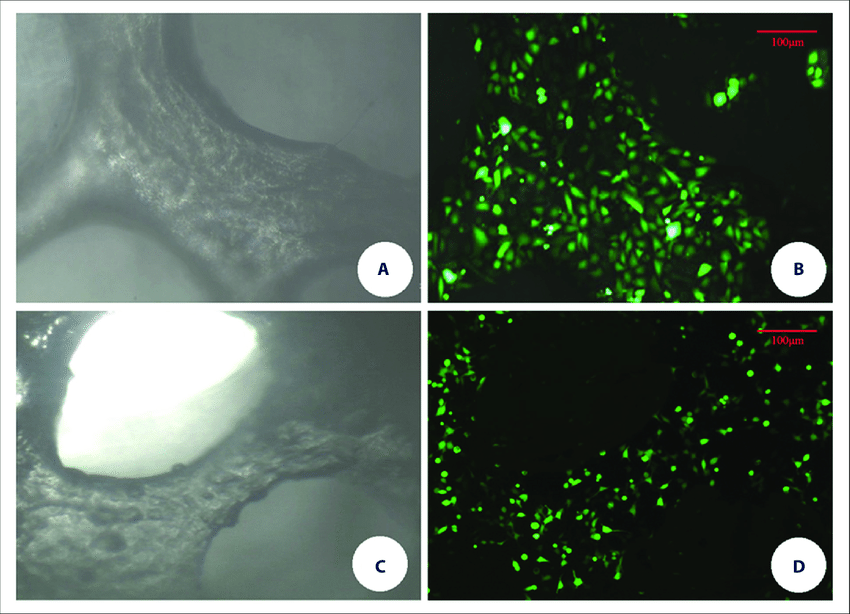
\includegraphics[width=0.6\textwidth]{figs/Light-microscope-and-fluorescence-microscope-observation-of-DBM-scaffolds-under-dynamic.png}
    \caption[Visual comparison between light and fluorescence microscopy]{A comparison between light (left sub-figures) and fluorescence (right sub-figures) microscopy. The same specimen is represented using each microscopy type with the top pair (A,B) and the bottom pair (B,D) each representing different cell cultures\cite{microscopeTypeFig}.}
    \label{fig:microscopeTypeCompare}
\end{figure}

\subsection{Factors regarding fluorophore selection for fluorescence microscopy}\label{sec:FluoroProcess} 
As described in Section \ref{sec:lightVsFluoro}, the primary reason to use fluorescence microscopy is the ability to select structures or biomolecules that are relevant to the analysis through the use of specific fluorophores. When imaged the indicated objects appear with greater clarity and differentiation than in optical microscopy through the rejection of irrelevant fluorescence. These benefits are not acquired without a cost which is the added decision-making of selecting suitable fluorophores for the analysis being performed. There are a number of factors involved in this can be viewed as the types of biomolecules being stained (for our mitophagy imaging purposes it is the organelles) and the fluorophore properties.\par Regarding the impact on fluorophore selection the largest is based on what biomolecules or structures are of interest to the analysis as the scope of fluorophores will be narrowed to those that suitably stain them after which the fluorophore properties are to be considered in the context of the imaging requirements. Imaging requirements can describe the status of the specimen whether alive or fixed; the duration of the imaging whether time-lapse is being performed; the desired signal strength of the captured fluorescence; and the number of fluorophore types employed such that the different types of structures of interest can be differentiated between.\par The fluorophore properties that will be explored are the excitation spectrum, the emission spectrum, the photostability, the maturation time, and the emission brightness~\cite{fluorophorePick, fluoro_properties_2, fluorophore_article}.

\paragraph{Excitation spectrum} is the range of wavelengths that are able to excite the indicators to induce emission. The excitation spectrum of a fluorophore must be evaluated relative to the microscope filters for the illuminant and the excitation spectra of indicators for other structure types. When the excitation spectra of two or more different fluorophores overlap, a phenomenon called `cross-talk' is induced~\cite{Bolte-2006}. This overlap can be complete or partial where the quantity of overlap can increase the severity of the cross-talk where cross-talk causes the simultaneous excitation of multiple fluorophores where only one fluorophore type was intended to be excited.
\paragraph{Emission spectrum} is the range of fluorescence wavelengths that the fluorophore emits post-excitation. This spectrum must be evaluated relative to both the filter preceding the photon detector and the emission spectra of different fluorophores employed for other structure types. When these emission spectra experience some quantity of overlap a phenomenon called `bleed-through' occurs~\cite{Bolte-2006}. Bleed-through where fluorescence captured by the microscope that is expected to be from a specific fluorophore is intruded by the fluorescence of unintended fluorophores interfering with the accurate differentiation of structures since structures can be incorrectly labelled as a structure due to this inappropriate emission spectra overlap. In fluorescence microscopy, it is standard to separate captured fluorescence wavelengths by channels thus grouping different structures under different channels when there is minimal bleed-through.
\paragraph{Photostability} is the property of the fluorophore's resistance to degradation due to photobleaching (will be discussed in Section \ref{sec:ConstraintsMicrosc}) which is a phenomenon that limits the total quantity of excitation that indicators can undergo. A higher photostability must be considered when indicators must undergo extended excitation such as time-lapse imaging (to capture temporal behaviours) or when a longer exposure time is required for the captured fluorescence to compose a sufficient signal~\cite{fluorophore_article}.
\paragraph{Maturation time} is the time required before the fluorophore begins fluorescence. This is exclusive to fluorescent protein-type fluorophores and the maturation time begins once the fluorescent proteins have been introduced (transfected) to the specimen~\cite[p.286-289]{matureFluoro}.
\paragraph{Emission brightness} is the property describing the potential intensity of the fluorescence emission relative to the intensity at which it is excited~\cite{fluorophore_article, fluorophorePick}. In this use, intensity refers to the number of photons either absorbed or emitted within some time window. This is under the assumption of optimal wavelengths as the effectiveness of the photon absorption is determined by the wavelength of the excitation photons based on the excitation spectrum and the number of photons of a specific wavelength will be relative to the emission spectrum of the fluorophore. Due to this it is more likely to induce greater excitation in a fluorophore for certain wavelengths and the brightness of the emitted signal will be greater in certain wavelengths than others. A higher emission brightness property means that lower total excitation experienced by the fluorophore is needed to emit a strong fluorescence signal than a fluorophore with a lower emission brightness. This is beneficial for time-lapses or when the photostability is low as less intense excitation energy is needed to capture a sufficient signal reducing the photobleaching experienced.\par
\textcolor{red}{I tried to describe this in a simple way without plagiarising the text and while avoiding the heavily mathematical definition. This was intended to remain high-level but I fear I may have still overcomplicated it.}

%The indicators each have excitation and emission spectra which characterise the frequencies of light required to excite the indicator and the frequencies of light emitted by the indicator post-excitation. The light intensity required for the excitation of and the emission from the indicators is distributed across these frequency spectra and the excitation and emission wavelength characteristics describe where the peaks of these respective spectra are situated. This means that for an indicator any excitation light with a wavelength within the excitation spectrum will induce excitation but the relative intensity of this excitation is dependent on the specific wavelength where the peak excitation will be situated at the spectrum peak. This means that to induce excitation an excitation light of a wavelength closer to the excitation peak will induce excitation quicker which is denoted as the `excitation wavelength' for a given indicator. This is similar to the emission spectrum save that the intensity of the emission fluorescence will be distributed across an emission spectrum with the maximum intensity being situated around an emission spectrum peak which is denoted as the `emission wavelength'.\par Excitation and emission spectra are of great importance when more than one indicator is applied where each indicator is intended to indicate different types of structures where these different types of indicated structures will be referred to as "indicated groups" for the remainder of Section \ref{sec:fluorMicr}. An example of these indicated groups can be two different types of organelles such as mitochondria and autophagosomes where an indicated group is composed of multiple independent mitochondria across the specimen that are targeted by the same fluorophore as they all meet the conditions required for the said indicator to bind to them. The impact of the excitation and emission spectra on the specimen imaging determines the separability of these indicated groups throughout the imaging process based on the overlap of these spectra between different indicators. Between multiple indicators when the excitation spectra and emission spectra overlap the phenomenon is referred to as `cross-talk' and `bleed through'~\cite{Sanderson-2014, crosstalk} for the overlap of excitation and emission spectra respectively. This phenomenon imposes a negative influence on the effectiveness of fluorescence microscopy and the implications of this will be discussed further in Section \ref{sec:ConstraintsMicrosc}. To mitigate the influence of cross-talk and bleed through it is important to maximise the distance between the excitation and emission spectra for all employed indicators in the imaging process.\par Photostability is the measure of the resistance to photobleaching for a given indicator. Photobleaching refers to a degradation in the indicator where this degradation proportionally reduces the fluorescence capabilities of the indicator~\cite{fluorophorePick}. This degradation is a natural byproduct of the excitation and emission process undertaken by indicators. Due to this, the suitability of the indicator photostability is dependent on the expected excitation duration, whether continuously excited or an accumulated duration due to multiple excitation periods, which can constrain time-sensitive observations if unsuitable. These time-sensitive observations can either entail time-lapse observations if the analysis requires a temporal resolution, where time-relative behaviours are captured over a period, or imaging with longer excitation exposure times to increase indicator excitation thereby inducing an increase in the total excited photon emission to accumulate into a sufficient fluorescence signal.\par The maturation time of the fluorophore (indicator) is exclusive to protein-based fluorophores that undergo a development process in order to achieve sufficient fluorescence ability prior to which fluorescence was not occurring or the occurrence of which was negligible. This development process is called the maturation process and it is the time required for the indicator to reach a state where optimal emission is achieved. This is important for observations of specimens undergoing rapid changes as the delay in imaging, due to the maturation time, can lead to certain specimen developments being missed. The dependence on a shorter maturation time is less important for specimens expressing time-insensitive phenomena and for fixed specimens which experience no changes from the point of fixation~\cite{fluorophorePick, matureFluoro}.\par The emission brightness is the property measuring the efficiency of the excitation-to-emission relationship of the indicator. The excitation of the indicator is a state achieved when the indicator has absorbed photons of an appropriate wavelength corresponding to the excitation spectra and then some of this excitation energy is then emitted by the indicator as photons of a certain wavelength corresponding to the emission spectra. Indicators with a higher emission brightness require less excitation to emit photons at a count equal to an indicator with a lower emission brightness property and conversely a higher excitation is required. This can be viewed as the expected energy loss during this conversion process of absorbed excitation energy into released emission energy and the proportion of this energy loss is indirectly described by the emission brightness. This can be important as photobleaching is induced by excitation and emission thus reducing the required excitation intensity to achieve sufficient emission will reduce the risk of photobleaching as compared to indicators requiring greater excitation under the assumption that the photostability is the same for both hypothetical indicators~\cite{fluorophorePick}.

\subsection{Constraints on the performance of fluorescence microscopy}\label{sec:ConstraintsMicrosc}
%This section needs a new title. First list the shared shortcomings such as photobleaching (especially time lapse) and describe the impact of cross-talk and bleed-through mentioned in prior section. The diffraction will be a large component of this and needs a reference as well, perhaps DeconvolutionLab2 or some other paper where the PSF is discussed. Also mention the thickness limitation of specimens due to out-of-focus fluorescence in Wide-Field which Confocal mitigates with the focal plane shift + the pinhole. Mention though that there is still some out-of-focus fluorescence originating from structures closer to the focal plane. INCLUDE SOURCES!!! Look for some sources for these i.e. for out-of-focus fluorescence and the diffraction.
In comparison to light microscopy, fluorescence microscopy has many advantages in the visual labelling of structure types of interest and the removal of irrelevant structures which clutter the image but they are not without performance constraints. These constraints on the imaging performance are primarily due to the suitability of the fluorophores for the given analysis, the condition of said fluorophores and microscope resolving limits. Prominent constraints that will be discussed are bleed-through, photobleaching and diffraction. While both cross-talk and bleed-through were mentioned individually, in Section \ref{sec:FluoroProcess}, they will be discussed together as the occurrence of both phenomena is required for the effect to be noticeable to the imaging quality. 

\paragraph{Bleed-through} and by extension \textbf{cross-talk}, are referred to either interchangeably~\cite{Sanderson-2014} or individually~\cite{Bolte-2006} depending on the source of the description. What can be seen is that both phenomena must occur simultaneously for there to be some impact since the overlap in emission spectra means little if only the intended fluorophore is excited given that the excitation spectra are fully separated. The benefit of segregating the employed fluorophores by the respective emission wavelengths is so that the different types of structures or biomolecules (e.g. types of proteins, certain organelles, etc.) can be differentiated easily. For this to function, there is the expectation that each structure type that is to be differentiated between has a `unique' emission wavelength, among the emission wavelengths used in that imaging, to identify it~\cite{Bolte-2006}. Bleed-through and cross-talk break down this emission wavelength uniqueness thus fluorescence expected to identify only structures of type A (e.g. mitochondria) will also capture structures of type B (e.g. lysosomes). This is avoided by minimising the overlap between the excitation spectra of different fluorophores and likewise for the emission spectra respectively since emission requires excitation and filters can be employed to reject small overlaps (typically occurring along the outer edges of the spectra) by filtering out the edges of the emission and excitation spectrum. This is also not without repercussion as some of the excitation and emission energy will be at these filtered regions reducing the total captured signal strength.\par
\textcolor{red}{The above paragraph is where I noticed the space after the paragraph heading. There used to be a comma after ``bleed-through'' but it was not flush with the word so I removed it.}
%\paragraph{Cross-talk} introduces uncertainty into this aforementioned structure-channel relationship when the underpinning expectation of this relationship, different fluorescence channels corresponding to specific structures, no longer holds true. The reason for this is that the channel label, expected to represent only a specific type of biological structure, becomes associated with structures outside of what was expected. This occurs when the emission and excitation spectra of the indicators overlap such that the fluorescence corresponding to some set of biological structures intrudes into the channel relating to a different set of structures. This can be mitigated through the use of filters specific to the channel wavelength being captured to minimize spectral overlap but the greater the number of channels being captured then the narrower the bandwidth for emission detection and the lower the intensity of each channel since the emission intensity is distributed across the spectrum~\cite{Bolte-2006, Sanderson-2014}. This is why it is important to maximise the distance between excitation and emission spectra of fluorophores and if possible to select narrower spectra to minimise this overlap although in practice even if the spectra are distant there is still technically some cross-talk although of such low magnitude that it is negligible.
\paragraph{Photobleaching} is the degradation of the fluorophore's ability to fluorescence due to exposure to light\cite{photobleach_excite, photobleachingPaper}. Despite this, it is the exposure to excitation-inducing light that contributes the majority to this degradation~\cite{photobleach_excite} with the exposure measured by the number of absorbed photons in this context. Since the excitation light intensity exposes the fluorophore to more photons within a given time frame while exposure duration extends the length of said time frame. Photostability is the property measuring the resistance of the fluorophore to photobleaching while the emission brightness defines the number of photons emitted by the fluorophore relative to the number of absorbed photons thus high emission brightness means lower intensity excitation needs to be applied to capture sufficient signal thus reducing photobleaching indirectly~\cite{Sanderson-2014}.

\paragraph{Diffraction} is a phenomenon experienced by photons due to their intrinsic particle-wave nature. This diffraction occurs when the photons travel through a small opening, such as a microscope aperture, and the photons are dispersed in a radial pattern originating from said opening. This radial pattern can also be visualised as a wavefront with amplitude oscillations originating from the opening with the pattern expanding outwards~\cite{Diffraction_Patterson}. 
Under the assumption that diffraction does not occur then each point of fluorescence emitted by the specimen, within the microscope resolution, is captured by the microscope with a corroborating fluorescence point across the image pixels. With diffraction, each of those points will have their intensity distributed radially around them distorting the spatial representation of the specimen in the image. This radial distribution oscillates in intensity as it radiates outward due to the amplitude oscillation of the wavefront which appears as concentric rings and can be referred to as the airy disk~\cite{Diffraction_Dedecker}. There is also some decay in the intensity of the rings successively but this reduction is non-linear and a few bright rings or none at all will be visible depending on the diffraction pattern. The diffraction pattern itself regarding both the size and the distribution in intensity across the successive rings is dependent on a number of properties but namely the size of the numerical aperture (NA) and the emission wavelength value~\cite{Diffraction_Patterson}.\par As stated prior, this diffraction distorts the spatial representation of the captured fluorescence by scattering the fluorescence signal across diffraction regions. This distortion can be reduced by reconstructing the image without diffraction through deconvolution (described in detail in Section \ref{subsec:Decon}) but the diffraction present in the image has to be understood for it to be reversed. This can be estimated through investigation of the image diffraction but this involves human bias leading to inconsistency in the results or a mathematical representation called a point spread function (PSF) can be generated using parameters specific to the imaging. The problem is that irrespective of the diffraction being correctly modelled is that the overlapping of diffraction regions beyond a certain amount makes reconstruction impossible for those regions. When these diffraction regions overlap the airy disks compound on each other resulting in a region that fits no diffraction pattern and cannot be reversed. This adds to the resolution limitation of microscopes as the diffraction pattern overlap from the airy disk centre to the first ring from the centre is roughly when effective reconstruction becomes impossible for those regions~\cite{Diffraction_Dedecker, Diffraction_Patterson}.

\subsection{Confocal Microscopy}\label{sec:Confocal}

\begin{figure}[h]
    \centering
    \subcaptionbox{Axial axis relative to Objective, Specimen and Specimen Stage. The Lateral Slice is annotated by a dashed red line\label{subfig:SideView}}[0.45\textwidth]{%
    \input{figs/Microscope Perspective.tikz}
    }%
    \hfill
    \subcaptionbox{The lateral view of the specimen as scene in the axial direction from the Objective.\label{subfig:topview}}[0.45\textwidth]{%
    \input{figs/Lateral Perspective.tikz}
    }%
    \caption[Two diagrams of different perspectives to view the specimen relative to the microscope objective. This is presented to show the relative position of the lateral slice (focal plane) in the specimen]{Two diagrams illustrating the two perspectives with the appropriate axis. \subref{subfig:SideView}) depicts the specimen from the side to display the hypothetical position of the lateral slice (focal plane) relative to the microscope objective with the $z$-axis, or axial direction, annotated perpendicular to the specimen stage. \subref{subfig:topview}) depicts the specimen as seen from the objective and will be referred to as the "Lateral Perspective" which views the $x,y$-axis of the specimen.}
    \label{fig:micro_persp}
\end{figure}

\paragraph{Microscopy thus far} The microscopy that has been discussed thus far (Section \ref{sec:lightVsFluoro}) has involved the illumination of the entire specimen and the subsequent capture of all fluorescence emissions, or reflections in the case of optical, limiting the clarity of the captured image by the specimen thickness and is called wide-field microscopy. Before exploring why specimen thickness is a detriment to the image quality the focal plane will be defined in the context of this section to simplify further explanations. The focal plane is a lateral plane perpendicular to the objective lens and light originating from along this plane is in focus thus providing a sharper image with greater clarity. An example of the focal plane can be seen in Figure \ref{subfig:SideView} and is referred to as ``Lateral Slice'' and light originating from above or below this plane is referred to as out-of-focus light~\cite{Sanderson-2014}. While wide-field fluorescence microscopy (often Epifluorescence microscopy) can discriminate between fluorescence based on wavelength through the use of filters, separating fluorescence representations of the specimen into groups, it cannot spatially discriminate between light originating from inside or outside of the focal plane. This results in the out-of-focus fluorescence being layered atop the in-focus fluorescence causing blurring and the loss of resolution of details (the pixel resolution is unchanged)~\cite{Sanderson-2014, confocal_modern}. Thicker specimens have larger volumes outside of the focal plane that will contribute more out-of-focus fluorescence thus limiting the image quality by the specimen thickness. An indirect repercussion of this lack of spatial discrimination of fluorescence by focus is that 3D images cannot be captured at high quality since an accurate volumetric representation of the specimen only functions under the assumption that the position, size and shape of specimen objects are accurately reflected in the image which out-of-focus fluorescence prevents.

\paragraph{Confocal microscopy} A solution to this is the use of confocal microscopy which is a microscopy architecture which employs a pinhole aperture before the photon detector to reject out-of-focus fluorescence, a comparison between wide-field and confocal imaging of a specimen is shown in Figure \ref{fig:widevsconfocalfig}. This rejection using the pinhole aperture works due to fluorescence emitted from different depths through the specimen approaching the pinhole at different angles after refracting through the objective and microscope lenses. This allows the imaging of cross-sections through thicker samples since the problematic out-of-focus fluorescence is rejected, or at least reduced. The implementation of a pinhole is not the sole addition to confocal microscopy, compared to wide-field, as the excitation and capturing of fluorescence originating from a singular point along said the focal plane is the second characteristic. The reason behind this asymmetry in focus across the focal plane is due to the pinhole rejecting fluorescence originating from a specific position and while depth is the major contributor to this so too is lateral position relative to the point of focus of the objective~\cite{Confocal-2005, confocal_modern}. When the pinhole rejections fluorescence it essentially rejects photons from the detector which are used to construct the image and insufficient photons lead to a weak image signal despite there being less noise from out-of-focus fluorescence leading regions closer to the focal point along the plane to diminish in intensity inversely to their distance from said point.\par Using `Confocal Laser Scanning Microscopy' (CLSM) as an example a scanning mirror is used at the objective lens to scan the focal point along the focal plane, maximising the acceptance through the pinhole of fluorescence from that point, while also focusing a high-intensity excitation laser to that same point~\cite{confocal_modern}. The high-intensity laser compensates for the loss of signal intensity due to pinhole rejection while the scanning of the focal plane point-by-point constructs a final image with the focus across the image being relatively uniform. This is only one such architecture with `Spinning Disk Confocal Microscopy' (SDCM) being another such confocal architecture employing multiple pinholes and scanning points, instead of the one in CLSM, but this will not be explored further in this text~\cite{Sanderson-2014, Confocal-2005, confocal_modern}. With the ability to reject out-of-focus fluorescence comes the opportunity to construct 3D images of the specimen which is performed by adjusting the depth of the focal plane and imaging individual lateral slices through the image while maintaining that only objects located at that depth in the specimen are captured in the corresponding slice of the 3D image. One point of consideration is that higher excitation laser intensities and the duration the laser dwells on a point can render a stronger image signal but the trade-off is that photobleaching is worsened and while the excitation is focused on a single point this laser penetrates through the depth of the specimen exciting out-of-focus points introducing photobleaching without capturing that fluorescence. This penetration through the depth of the specimen by the laser is the limiting factor on the volumetric resolution of the image along the depth as each lateral slice will require an additional excitation to pass along the focal plane increasing photobleaching throughout the image. The size of the pinhole determines the strictness of the out-of-focus fluorescence rejection but it also determines the loss of signal intensity from the emitted fluorescence. Increasing the excitation laser intensity or extending the duration the excitation laser dwells on each point can increase signal intensity but worsens photobleaching thus a compromise must be made when imaging in 3D.\par
\textcolor{red}{I rewrote this description of Confocal microscopy in the hope that it flowed better and used simpler language than before. I have three sources explaining Confocal microscopy but how do I avoid citing every line? Can I cite at the end of a paragraph or can I cite the key point while assuming the reader will realise the point built upon that subsequently relied on the same source?}

%Confocal microscopy is a variation of wide-field microscopy that enables the imaging of a specimen from a 3D perspective and allows observations of the specimen at specific depths through the specimen to be sampled with greater clarity. In reference to Figure \ref{fig:micro_persp}, two perspectives of the specimen can be seen relative to the objective. The perspective from the objective, Figure \ref{subfig:topview}, is the lateral view and is the perspective from which all wide-field microscopy typically images the specimen. The specimen is imaged at specific lateral slices where a lateral slice is a view from the aforementioned lateral perspective and is situated at some depth through the specimen along the $z$-axis as depicted in Figure \ref{subfig:SideView}. An example of a lateral slice is shown in Fig. \ref{subfig:SideView} with a dashed, red line and the position of this lateral slice can be shifted along the $z$-axis. Imaging multiple lateral slices sequentially through the specimen depth, along the $z$-axis, compose a volumetric representation of the specimen providing greater spatial resolution of the specimen.\par In wide-field microscopy the specimen is imaged from the lateral perspective, shown in Fig. \ref{subfig:topview}, but the depth cannot be selected thus all fluorescence throughout the specimen is captured. In thin specimens, this is not as problematic but as specimen thickness increases so too does the challenge in diffraction mitigation where overlapping diffraction regions increase the difficulty in reconstructing the original fluorescence prior to diffraction. This diffraction-related reconstruction issue is mentioned in Section \ref{sec:ConstraintsMicrosc} where the distance between indicators is not just the lateral distance (relative to $x,y$-axis shown in Fig. \ref{subfig:topview}) but also the $z$-axis distance between indicators.\par Confocal microscopy mitigates this through lateral slice isolation where a currently selected lateral slice is referred to as the focal plane and all the fluorescence emitted from indicators positioned along this slice is brought into focus. When the specimen is excited fluorescence is emitted by indicators both inside and outside of the focal plane such that after passing through the objective lens the angle of trajectory of said fluorescence changes based on the depth of the indicators. Prior to the photon detector, which captures this fluorescence, is a pinhole opening and based on the pinhole dimensions only fluorescence approaching from a certain range of angles can pass through this pinhole. From this, it can be said that the focal plane is rather the lateral slice from which fluorescence originates that approaches the pinhole at the correct angles to pass through. In summary, fluorescence outside of the focal plane is mitigated, if not outright rejected, thus reducing the potential conflict of diffraction in the $z$-axis and isolating only the fluorescence representing that slice and fluorescence originating from outside of the focal plane is referred to as out-of-focus fluorescence~\cite{Sanderson-2014}.\par While the pinhole aids image quality by only capturing fluorescence close to the focal plane the quality of the lateral slice itself is not improved further. To further improve the lateral slice clarity each point of the lateral slice is captured and constructed into a final lateral slice image. This is performed by scanning the excitation light across points of the specimen along the lateral plane thus only exciting the specific points of the specimen. This allows the capturing of singular points of excitation along the specimen which is used to construct the full resultant image and means that the image region can exceed that of traditional wide-field microscopy as the final image can be compiled from a wide scanned area. This scanning process is achieved by the implementation of adjustable mirrors that direct the excitation laser along the specimen thus the rest of the apparatus can remain stationary~\cite{Sanderson-2014, Confocal-2005}. Through the use of both laser scanning and the pinhole, highly detailed lateral slices at varying depths of the specimen can be imaged while addressing out-of-focus fluorescence and enabling improved spatial resolution as three-dimensional representations can be captured.\par These described benefits of confocal microscopy are not without shortcomings regarding the pinhole size and the laser scanning. The pinhole size has been stated to reduce out-of-focus fluorescence with the strength of this reduction inversely proportional to the pinhole size where a smaller pinhole will reduce more of the out-of-focus fluorescence but also, less so, the in-focus fluorescence. This engenders a balancing act where greater reduction will remove further out-of-focus fluorescence but the loss of in-focus fluorescence will result in less fluorescence being captured resulting in a weaker image signal. A potential solution to this is to increase the laser intensity or exposure time to provide further in-focus emission photons to strengthen the signal but this can in turn induce more photobleaching. The shortcoming of laser scanning is more based on the scanning method employed, of which there are multiple, but traditional high-intensity laser scanning can be time expensive relative to the image resolution, different to the optical resolution of the photon detector, as a greater number of points construct said image. The dwell time of the laser to increase excitation exposure also factors into this scanning duration and returns to this balancing act~\cite{Sanderson-2014}. One last statement is the impact of three-dimensional spatial resolution on the photobleaching risk of the specimen. This scanning laser only excites a single point relative to the lateral perspective but descends through the full depth of the specimen, with the out-of-focus fluorescence mitigated, but for each lateral slice captured each of these points along the depth will be repeatedly exposed increasing the photobleaching damage as further slices are captured~\cite{Sanderson-2014}. An example of a specimen captured through the use of both wide-field and confocal microscopy can be seen in Fig. \ref{fig:widevsconfocalfig} where the benefit of out-of-focus rejection is visible in the confocal image improving the clarity of the imaged specimen.
%Ask Rensu for advice on wording for focal plane (particularly the mess that is the lateral plane description) and find sources to corroborate that this is a standard. For the photobleaching refer to http://cshprotocols.cshlp.org/content/2014/10/pdb.top071795.full thoroughly as they describe dwell time and such. This is not the focus of your research and is merely to act as reasoning as to the z-axis resolution limits and speculative reasoning for some poor samples

\begin{figure}
    \centering
    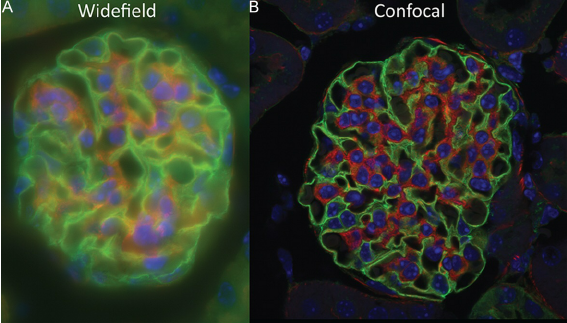
\includegraphics[width=0.8\textwidth]{figs/A-confocal-microscope-allows-you-to-do-optical-sectioning-in-thick-specimens-by-removing.png}
    \caption[A 2D image of a specimen retrieved using wide-field (left) or confocal (right) microscopy]{A 2D image of a specimen retrieved using wide-field (left) or confocal (right) microscopy \cite{specimenConfocalFig}}
    \label{fig:widevsconfocalfig}
\end{figure}

\subsection{Wide-field and confocal microscope apparatus}\label{sec:MicroAppa}
%Place this section after confocal
\begin{figure}[h!]
    \centering
    \subcaptionbox{Wide-Field Microscope\label{subfig:WFM}}{\includegraphics[width=0.28\linewidth]{figs/widefieldApparatus.jpg}}
    \subcaptionbox{Confocal Microscope\label{subfig:CM}}{\includegraphics[width=0.70\linewidth]{figs/confocalApparatus.jpg}}
    \caption[Diagrams representing the Wide-Field Microscope and the Confocal Microscope]{Diagrams representing the Wide-Field Microscope and the Confocal Microscope \cite{Sanderson-2014}}
    \label{fig:microscope_diagrams}
\end{figure}

Both wide-field and confocal microscopy are applications of fluorescence microscopy albeit with different microscope designs. The design aspects of both microscopes, seen in Fig. \ref{fig:microscope_diagrams}, are the use of filters for selecting both the excitation and emission wavelengths, the microscope objective lens and the excitation illuminant. The key components that differ are that wide-field frequently implements cube filters which both direct the excitation light to the specimen through the objective and the emission photons to the photon detectors. Filters within the cube filters select the relevant wavelengths when redirecting the light to the specimen and the detector. Conversely, confocal microscopes implement multiple adjustable, and fixed, mirrors in combination with filters. These mirrors allow the excitation laser to be directed to specific regions of the specimen and the resultant emission fluorescence reflects off of these mirrors on approach to the photon detector. The adjustment of the mirrors determines the angle at which the emission fluorescence approaches the photon detector based on the point of emission relative to the mirror angles. Confocal microscopy also uses a pinhole aperture before the photon detector which rejects photons depending on the angle at which they approach the pinhole. It is the combination of the adjustable mirrors manipulating the emission fluorescence angles with the pinhole that allows the reduction of emission fluorescence outside of the position of focus from reaching the photon detector. This position of focus can also be adjusted in depth using microscope apparatus allowing separated cross-sections through the specimen to be captured along the specimen depth. In the confocal microscope, the excitation illuminant is a precise laser as opposed to the wide-field illuminant which radiates across the whole specimen~\cite{Sanderson-2014}.\par
\textcolor{red}{This is one of the few subsections where I performed no revisions besides passing through it to check coherency. If you feel this section is unnecessary please let me know.}
\subsection{Summary}
Many aspects of fluorescence microscopy have been discussed ranging from some of the factors under which fluorophores (indicators) are selected to the decisions between the microscopy method applied. The key points covered are that different fluorophores bind to specific environments or subjects based on their chemical or biological composition; the selection of these fluorophores must consider their excitation and emission spectra to avoid overlap; confocal microscopy enables more detailed imaging with less out-of-focus fluorescence with the added option of three-dimensional imaging.
\textcolor{red}{I initially wrote this summary a year back and haven't done so for other sections. Do you think it would be beneficial to provide a short summary of a section at the end of a section or should I scrap the summaries as a whole? If I am going to keep summaries I feel I need to do it for every section out of consistency.} 

\section{Colocalization}\label{sec:coloc}
With the specimen imaged using fluorescence microscopy, as described in Section \ref{sec:fluorMicr}, mitophagy occurrence is to be measured. Through fluorescence microscopy, each of the organelle types has been separated by the selected fluorophore excitation and emission spectra such that a different colour channel can be assigned to each. Since mitophagy involves the engulfment of mitochondria by autophagosomes which fuse with lysosomes (becoming autolysosomes) it can be assumed that the overlap of mitochondria and autophagosomes (or lysosomes) would be a sufficient indicator of mitophagy. While this holds in a physiological sense, this is not guaranteed for the overlap of structures between two channels, one of which is the mitochondria channel, as that would imply that what was imaged is a perfect representation of the specimen organelles to the highest level of precision. While newer microscopy architectures and methods have increased in imaging resolution to older iterations the required resolution and precision increase as there are attempts to image smaller structures and objects with increased fidelity and detail. To compensate for this shortcoming in the image representation of the specimen a reliable framework is required to evaluate the overlap present by several factors and calculate the certainty that the perceived cross-channel overlap can be classified as colocalization~\cite{practical_guide_coloc}.\par In "A practical guide to evaluating colocalization in biological microscopy"~\cite{practical_guide_coloc} there is specific mention of two components which derive colocalization and they are co-occurrence and correlation. Co-occurrence is identical to the aforementioned overlap where the fluorescence from each channel occupies the same position in space. Correlation measures the intensities of the fluorescence between each channel relative to the distribution of these intensities over space. In combination, this results in colocalization being evaluated by not just the spatial co-occurrence of fluorescence channels in the image but also the proportion of fluorescence intensities between each channel at these regions of co-occurrence.\par While co-occurrence may be sufficient for visual evaluation of possible colocalization events it is an unreliable indicator of colocalization within the specimen as a qualitative measure of correlation is unintuitive and difficult. For this reason, there exist a number of algorithms which measure colocalization within the image region or a selected sub-region as true colocalization cannot be determined due to imaging limitations and the number of spatial characteristics describing colocalization being difficult to fully capture. Due to this many of these algorithms provide pros and cons based on the application. These pros and cons can range from intermediate values (between 1 and 0) being uncertain in interpretation, being sensitive to noise, or time-expensive iterations to converge to a reliable result~\cite{Bolte-2006}. The standard colocalization algorithms are Pearson's correlation coefficient, Manders' overlap coefficient, Manders' correlation coefficient, Costes' approach, Van Steensel's approach, and Li's approach~\cite{Bolte-2006, practical_guide_coloc}.\par These methods provide a numeric evaluation of the colocalization present in the analyzed region but due to the constraints present within these methods, they are typically applied to selected sub-regions as opposed to the full specimen image. When these regions contain multiple colocalization events these methods cannot distribute the calculated colocalization score between the events thus precise region is of greater importance to evaluate the colocalization measure of each region of co-occurrence. A recently developed method is that of Regression adjusted colocalisation colour mapping (RACC)~\cite{racc} which calculates the colocalization throughout the region (which can be the entire image) and outputs the specimen image (with both images overlaid) with a colocalization channel overlaid. This colocalization channel presents values proportional to the colocalization strength which is zero for regions without overlap but across regions of co-occurrence the provided value allows the colocalization strength to be spatially and visually mapped to these individual event locations within the specimen.
%Need to write a reduced section on Colocalization. Should be sufficient to only discuss colocalizing, RACC and briefly, BRIEFLY mention the other measurements but do not go into depth for them (RACC slightly can go into)

\section{Image preprocessing}\label{sec:image_prepro}
%Avoid going into techniques. This can be summarised as a filtering stage (containing background removal), deconvolution and thresholding. Leave the techniques for the implementation section as this is not a focal point and will be time demanding

With the specimen images acquired through microscopy, some of which are detailed in Section \ref{sec:fluorMicr}, the analysis of the features described by the image would ideally commence. As was introduced in Section \ref{sec:intro_noise}, it is not uncommon for the specimen representation captured in the image to deviate from the actual specimen due to the presence of noise, distortion or artefacts. In the context of noise, the quality of the image can be approximated as the similarity between the actual specimen and the structures of interest that may be labelled and what is described in the captured image.\par This actual specimen representation refers to the ideal visualisation of the specimen where stained structures and biomolecules of interest to the analysis are accurately differentiated as well as the size, shape and position of these captured in the image precisely reflect the matching objects in the real specimen. When there are components in the image that are not reflexive of the image then the image diverges from the specimen and the image degrades thus elements of the image causing this are referred to as degradation factors.

\subsection{Sources of interference in image quality}\label{sec:Noises} %This section needs to be reviewed fully with new understanding regarding what is of importance. We never deal with microscopic and photon noise as they form part of the background noise.

As mentioned prior, the correction of the image quality degradation is necessary for the accurate analysis of these microscopy images. The factors contributing to the degradation have been listed as distortion, noise and artefacts although there is a tentative degree of overlap between these. For clarity, the definition of distortion, noise and artefacts in the context of this research will be presented before future use.\par Distortion is the spatial deformation of the image signal such that the shape of the image signal and described features differ from the real subject. Noise can be visually described as perturbations of the captured structures in the image that reduces their clarity without presenting distinct structures (where distinct structures have shape and size similar to the structures of interest). Since noise is typically thermal or electrical in origin (from the microscope) the noise factor is applied to the image signal when captured and is applied across the entire image with the severity of this noise described as the ratio between the image signal power and the power of the noise termed as the signal-to-noise ratio (SNR). Artefacts are the last component and describe any aberration in the captured image signal such that distortion and noise could be categorized as types of artefacts. For this research artefacts will refer to visual aberrations in the image signal that are irregular and present with sizes and shapes closer to the structures of interest but typically are lacking in overall signal intensity at that focal plane. The severity of these artefacts is dependent on the similarity between them and the structures of interest and how close the average intensity of an artefact is to the average structure intensity. These artefacts originate from fluorescence that was not intended for capture (due to the occurrence of bleed-through); the fluorophore could be binding to biomolecules outside of expectation (e.g. binds to specific proteins but unexpectedly these proteins are found in both the cytoplasm and the organelle with the former being unexpected); or out-of-focus fluorescence from a currently out of depth structure has not been sufficiently reduced appearing as an artefact. This sounds similar to that of noise but rather these artefacts can originate from specimen elements that are not intended for capture yet are described, even weakly, within the image.\par With these research-specific definitions presented an overview of some of the origins of these image quality degradation factors is described below: 

\begin{itemize}
    \item \textbf{Microscope Noise}: This takes the form of Poisson noise and Gaussian noise contributed to the image signal through the photon detector by thermal and electrical noise originating from certain microscope components.
    \item \textbf{Photon Noise}: Due to the discrete particle nature of photons the quantity of photons emitted by excited fluorophores is not consistent. When this inconsistency in emission occurs there is in turn a variation quantity of photons detected by the microscope over a period of time. This culminates in the variance of the image signal strength, particularly for short imaging periods where a baseline expected photon count cannot be reliably determined to mitigate this variation. This variance visually appears as noise which is characterised in the image signal by a Poisson Distribution~\cite{Meiniel2018, PoisGauss}.  
    %\item Speckle Noise:
    \item \textbf{Microscope Diffraction}: As described in Section \ref{sec:ConstraintsMicrosc}, the fluorescence emitted by the specimen passes through an objective lens and a pinhole aperture both of which cause the photon signal, when viewed as a wave, to diffract. This diffraction induces a distortion of the image signal at the detector and can be characterized as a blurring radiating from each pixel. The severity of this distortion is relative to both the image signal conditions (e.g. emission wavelength) and the microscope apparatus (e.g. numerical aperture).
    %Need to refer to distortion here here
    \item \textbf{Background fluorescence}: As described in Section \ref{sec:ConstraintsMicrosc}, this is a broad category of fluorescence which has been unexpectedly captured and does not necessarily originate from the selected fluorophores in focus. This can contain auto-fluorescence, out-of-focus fluorescence, and bleed-through among many other possible environmental fluorescence.
    % Should refer to artefacts here in some capacity even minor
\end{itemize}

\subsection{Standard pipeline for image pre-processing}\label{subsec:pipe}
%The introduction already introduces the pipeline and preprocessing. This should be a shorter section providing greater detail and focus on the numbered list below. This will lead into the solutions section which are what are implemented in this pipeline
%Should reference Chaudhy here for a pipeline base
Specimens are imaged using microscopy to analyse and measure properties, activities, and behaviours related to the specimen. These specimens are imaged such that the visual features describing phenomena and characteristics can be measured for the appropriate analysis. As detailed in Section \ref{sec:Noises}, the reliability of these measurements is proportional to the image quality which is degraded by several factors. To restore image quality several methods can be applied which reduce the presence of these degradation factors. This phase of the image preparation before the analysis, but after imaging, during which these methods are applied is referred to as the pre-processing phase (introduced in Section \ref{sec:intro_noise}) where a number of these methods are applied sequentially. This sequential application of methods and techniques for image quality restoration is the pre-processing pipeline (introduced in Section \ref{sec:intro_prep_pipeline}) through which the output of each method feeds into the input of the next allowing the degradation reduction to compound along the pipeline. \par There are numerous different techniques which can be applied each of which addresses specific degradation factors and have conditions under which they perform optimally. It is for this reason that sequential application of methods is ideal as these techniques address different degradation factors but in the process of reducing these factors the image signal can get diminished if too aggressive (e.g. blurring structure edges during noise removal) or the performance of said techniques are sensitive to the presence of other factors. By sequentially applying these techniques preceding techniques can reduce factors while improving the conditions for proceeding techniques while proceeding techniques can compensate for the limitations of the prior techniques. For this reason, it is important to plan the techniques used and the aggressiveness at which each technique is applied to balance between image signal preservation and noise removal. For colocalization analysis (overview in Section \ref{sec:coloc}) in the context of the mitophagy research use case a high-level abstract pre-processing pipeline, based on the pre-processing employed by \cite{PipelineDecon-Chaudhry}, is presented: 
\begin{enumerate}
    \item The PSF for the image is generated based on the image metadata and the microscope used. This was mentioned in Section \ref{sec:ConstraintsMicrosc} and will be discussed in further detail in Section \ref{subsec:Decon}.
    \item Deconvolution is performed on the image utilizing the appropriate PSF. This will mitigate the distortion which occurs at the objective lens. The reason for deconvolution being applied so early will be discussed in Section \ref{subsec:Decon}.
    \item Filters and image enhancement is employed to maximize the image signal strength while diminishing, or removing, noise. Frequently employed noise removal can diminish signal across the image although more so for noise thus image enhancement restores the strength of the image signal. 
    \item Foreground and background segmentation. The removal of artefacts induced by background signals and uneven illumination that is both irregular and prominent for standard denoising to effectively mitigate.
\end{enumerate}
Further image segmentation techniques or analysis techniques would be employed after this to acquire the measurements from which to draw observations. For the mitophagy use case, these observations will typically relate to the conditions and behaviours of the imaged organelles concerning the mitophagy process. This is not definitive of all pre-processing pipelines but provides an example of the sequential order in which these methods are applied for effective image preparation.

\subsection{Overview of the methods to restore image quality}\label{sec:overview_preproc_methods}
As discussed in Section \ref{subsec:pipe} prior, several techniques are applied sequentially to the image to restore the image quality. These techniques will be categorized (for this research) by the effect they have on the image. The groups will be deconvolution, denoising, image enhancement and thresholding. 

\subsubsection{Deconvolution}\label{subsec:Decon}
%Make sure the relation of the PSF to the NA of the objective and the emission wavelength is important as that is the wavelength that the dispersed spectrum is centred around and is important to reconstruct the original channel fluorescence.
During the imaging process, there is some degree of expected blurring of the image due to diffraction. This was described in detail in both Sections \ref{sec:ConstraintsMicrosc} and \ref{sec:Noises} where diffraction is the phenomenon where light scatters after passing through an aperture leading to the fluorescence spreading from singular points. This spread is more visible when it originates from brighter points thus structures with strong image signals present more prominent spreads which appear as blurry regions surrounding the original structure. This is problematic as this distorts the actual spatial representation of the imaged objects as they may appear larger than they are and the overlapping of these blurred regions can obfuscate edges and fine details thereby reducing the image quality. A technique known as deconvolution can be applied to the image after imaging which works to reverse the diffraction phenomenon but this requires the diffraction pattern for the image to be known and it is for this reason that overlap between diffraction blurs can interfere with effective reconstruction.\par The diffraction pattern can be determined in several ways but a convenient and effective method is to determine the theoretical diffraction pattern by calculating the PSF. The PSF is a mathematical model of the diffraction pattern that while lacking the nuance of the actual pattern is similar enough for effective deconvolution. The PSF calculation considers several imaging and fluorophore properties such as the relationship between the image pixel size to real distance in nm, the NA, the emission wavelength, the refractive index, the distance between lateral sections in 3D images and the microscope optical model among other properties~\cite{psfgen} with an example of a generated PSF shown in Figure \ref{fig:psf_example}.
\begin{figure}
    \centering
    \subcaptionbox{First PSF slice\label{subfig:first_psf}}{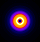
\includegraphics[width=0.27\linewidth]{figs/ch2figs/psf1.png}}
    \subcaptionbox{Second PSF slice\label{subfig:second_psf}}{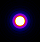
\includegraphics[width=0.27\linewidth]{figs/ch2figs/psf2.png}}
    \subcaptionbox{Third PSF slice\label{subfig:third_psf}}{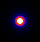
\includegraphics[width=0.27\linewidth]{figs/ch2figs/psf3.png}}
    \caption[PSF example for a 6 slice 3D image]{PSF example for a 6 slice 3D image. The PSF is mirrored between the first three and last three slices thus only the first three are shown and the order is inverted for the next three. The slices (\subref{subfig:first_psf})-(\subref{subfig:third_psf}) are ordered by depth where the later in the order the deeper the slice.}
    \label{fig:psf_example}
\end{figure}
\par In the theoretical pipeline described in Section \ref{subsec:pipe} the first step is to determine the PSF and the second is to apply deconvolution after which further processing can be applied. To justify this order first a simple algebraic representation of the captured image in relation to the blurring is shown~\cite{6505824, DeconLab2}:
\begin{equation}\label{eq:blurAdded}
    G(x,y) = F(x,y)*S + \eta(x,y)
\end{equation}
Where $G$ is the captured distorted image, $F$ is the original undistorted image signal, $S$ is the representation of the diffraction and the additive white noise is represented by $\eta$. The additive white noise is usually Poisson/Gaussian and originates from electrical or thermal energies in the microscope detector and apparatus. From \ref{eq:blurAdded}, the culprit of the distortion can be seen as $S$ which is also the PSF and the original image $F$ is convolved with the PSF to result in the distorted captured image. To reconstruct the original image $F$ a deconvolution operation needs to be applied with the appropriate PSF to `reverse' the diffraction effect of the microscope pinhole.\par
\begin{equation}\label{eq:psf_added}
    F(x,y) = G(x,y)*H(S^\ast)
\end{equation}
Where $H()$ is the deconvolution function and $S^\ast$ is the determined PSF for the image. Depending on the method by which the PSF is calculated, and when, the selection of what algorithms to apply to the image before deconvolution is significant. Operations that change the image signal, particularly in a non-linear or adaptive local approach such as Gaussian blurring, can lead to changes in the dispersion of the image signals within the image and thereby change the properties of the blur. If the PSF is generated so that these adjustments can be compensated for then this may be of little concern but if the PSF cannot do so then applying other algorithms before deconvolution could introduce unexpected outcomes and risks.\par Regarding the additive white noise, it is not uncommon for deconvolution algorithms to also remove noise~\cite{PipelineDecon-Chaudhry} and since the additive white noise is theoretically independent of the image signal distortion then denoising algorithms targeting solely the additive white noise could be applied with minimal issue.\par There are multiple deconvolution algorithms which can be used such as Richardson-Lucy, Richardson-Lucy Total Variation, Tikhonov Regularization Inverse Filter, Tikhonov-Miller and Regularized Inverse Filter to name a few~\cite{DeconLab2}. The two primary groups of deconvolution algorithms are iterative methods, such as Richardson-Lucy, and inverse methods, such as Tikhonov Regularization Inverse Filter. In Figure \ref{fig:deconvolution_showcase} the effects of deconvolution are shown with a comparison of before and after the application. The pre-deconvolution image (Fig. \ref{subfig:preDecon}) shows how the diffraction induces a blurred region distorting the perceived volume and shape of structures in the image as was discussed prior.

\begin{figure}[h!]
    \centering
    \subcaptionbox{Specimen image pre-deconvolution\label{subfig:preDecon}}{\stackinset{r}{}{t}{}{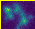
\includegraphics[width=0.1\linewidth, cframe=orange 2pt]{figs/ch2figs/Cropped_before_decon.png}}{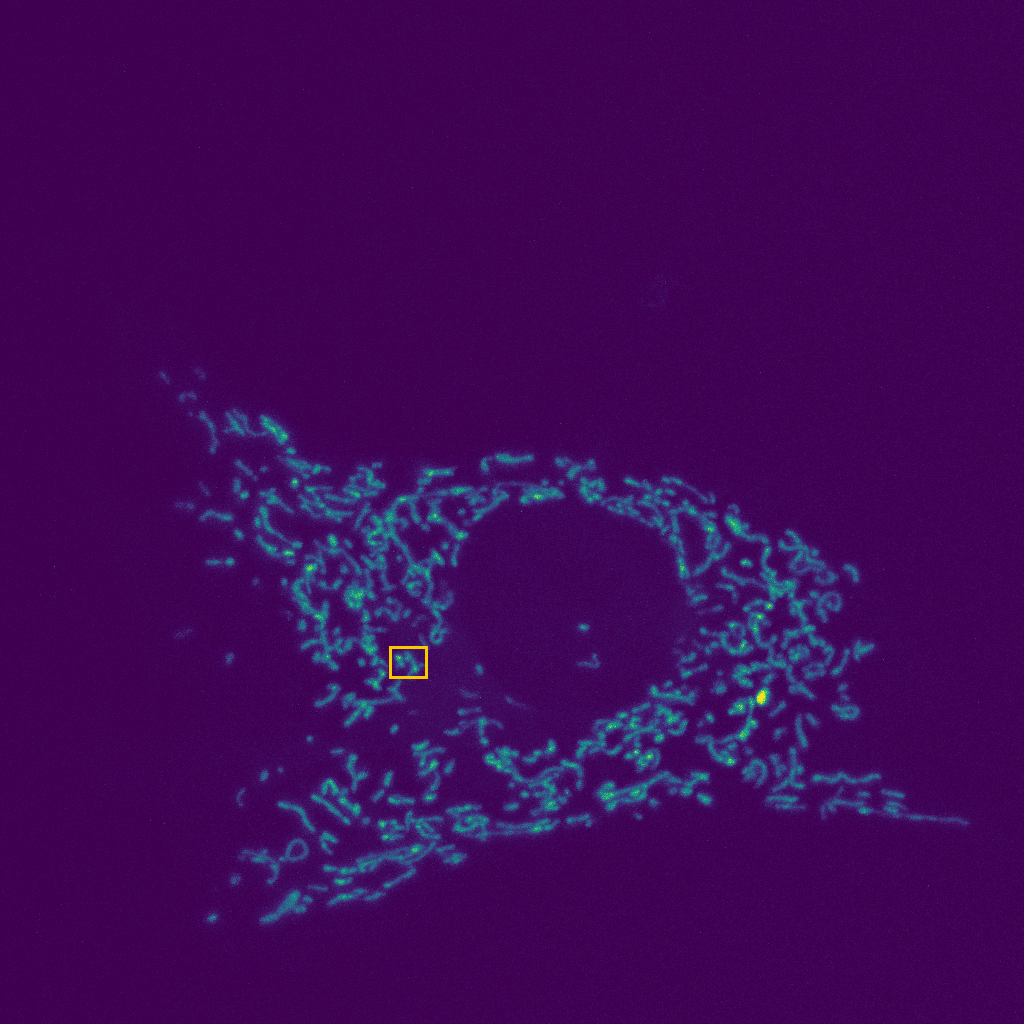
\includegraphics[width=0.49\linewidth]{figs/ch2figs/MAX_N1CCCP_1C=1_raw.png}}}
    \subcaptionbox{Specimen image post-deconvolution\label{subfig:postDecon}}{\stackinset{r}{}{t}{}{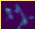
\includegraphics[width=0.1\linewidth, cframe=orange 2pt]{figs/ch2figs/Cropped_after_decon.png}}{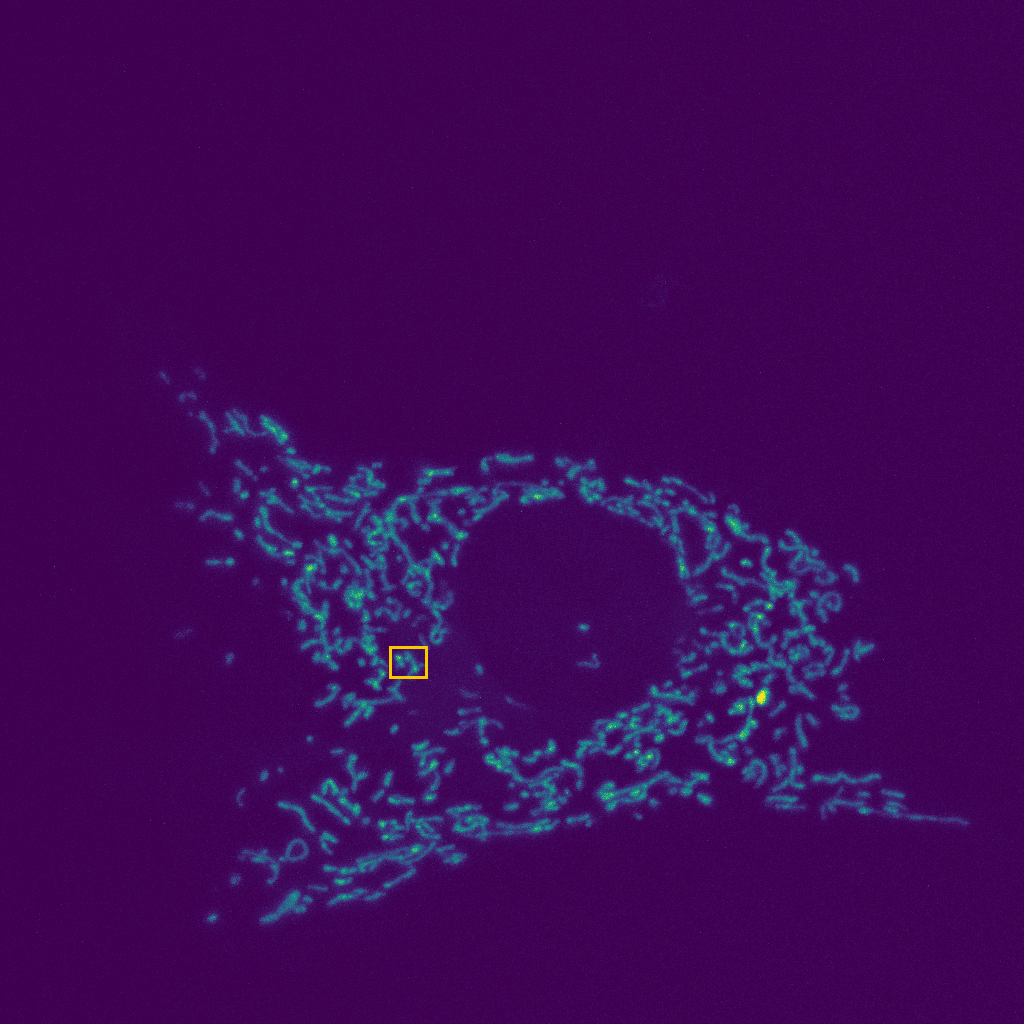
\includegraphics[width=0.49\linewidth]{figs/ch2figs/MAX_N1CCCP_1C=1_raw.png}}}
    \caption[Showcase of the effect of deconvolution on specimen images]{A maximum intensity projection of a specimen image is shown to compare \subref{subfig:preDecon}) pre-deconvolution and \subref{subfig:postDecon}) post-deconvolution. A region of interest that is zoomed-in is shown in the top right corner of each respective figure.}   
    \label{fig:deconvolution_showcase}
\end{figure}

\subsubsection{Denoising}
Denoising methods are transformations applied to the image to mitigate the presence of noise within the image. As detailed in Section \ref{sec:Noises}, regarding the degradation factors definitions, noise is generally expressed in the image as a global presence throughout the image which reduces the clarity of the features but typically does not generate new distinctive features. To clarify this, noise induces fluctuations in the amplitude of the image signal centred around the original signal and while these fluctuations are randomly distributed throughout the image they still follow certain `rules'. The fluctuations of individual pixels occur independently of other pixels yet the sign (positive or negative) and amplitude of all noise-based fluctuations across the image are drawn from the same distribution~\cite{bioimage_book}. There can be multiple noise fluctuations, with different origins, that compound in the resultant effect on the image pixels but the distributions from which these are drawn can be identical or different between different noise distributions. In an ideal situation, it may be possible to estimate the distribution of the noise from the image histogram but the compounding of other degradation factors on the image signal result in this being quite difficult for real image signals.\par Due to this methods that can mitigate the impact of the noise independent of knowing the noise distribution are necessary. These techniques are composed prominently of filter methods which are applied to pixel neighbourhoods and apply a filter operation. The filter operations can be standard mathematical operations, such as the median or mean of the neighbourhood, where the calculated value is applied to the pixel the neighbourhood is centred on. Irrespective of the exact filter method applied a consistent characteristic of denoising outputs is the smoothing of the image as can be seen in Figure \ref{fig:denoising_example} where the Sigma filter~\cite{sigma_filter}. As mentioned prior, many of these methods apply an operation to a pixel which adjusts the value based on the surrounding pixels thus reducing the variance within these neighbourhoods.\par While the discussion has been constrained to finite neighbourhoods there are also techniques which consider all pixels for the operation but the contribution of each pixel is relative to the distance from the pixel to be adjusted. This reduction in variance in image regions is fine for those already expressing a low variance but image features like edges are expressed by the relatively high variance localized around the edge. It is for this reason that excessive smoothing through denoising is detrimental for features expressed by high local variances limiting the quantity of denoising that can be applied~\cite{sigma_filter}. Likewise, even image regions that express limited variance may describe a feature yet excessive smoothing can eventually remove the boundary between the background and the objects to be analyzed. For this reason, denoising does have an upper limit on its application of it based on the noise level being too strong or the image signal being too weak. There do exist denoising methods optimized for edge preservation such as the Sigma filter~\cite{sigma_filter} but these, among the numerous other denoising methods, will not be explored in further detail for this work.

\begin{figure}
    \centering
    \subcaptionbox{Prior to denoising\label{subfig:before_denoise}}
    {\stackinset{r}{7pt}{t}{1pt}{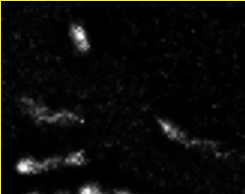
\includegraphics[width=0.15\linewidth, cframe=orange 0.5pt]{figs/ch2figs/Cropped_before_sigma.png}}{
    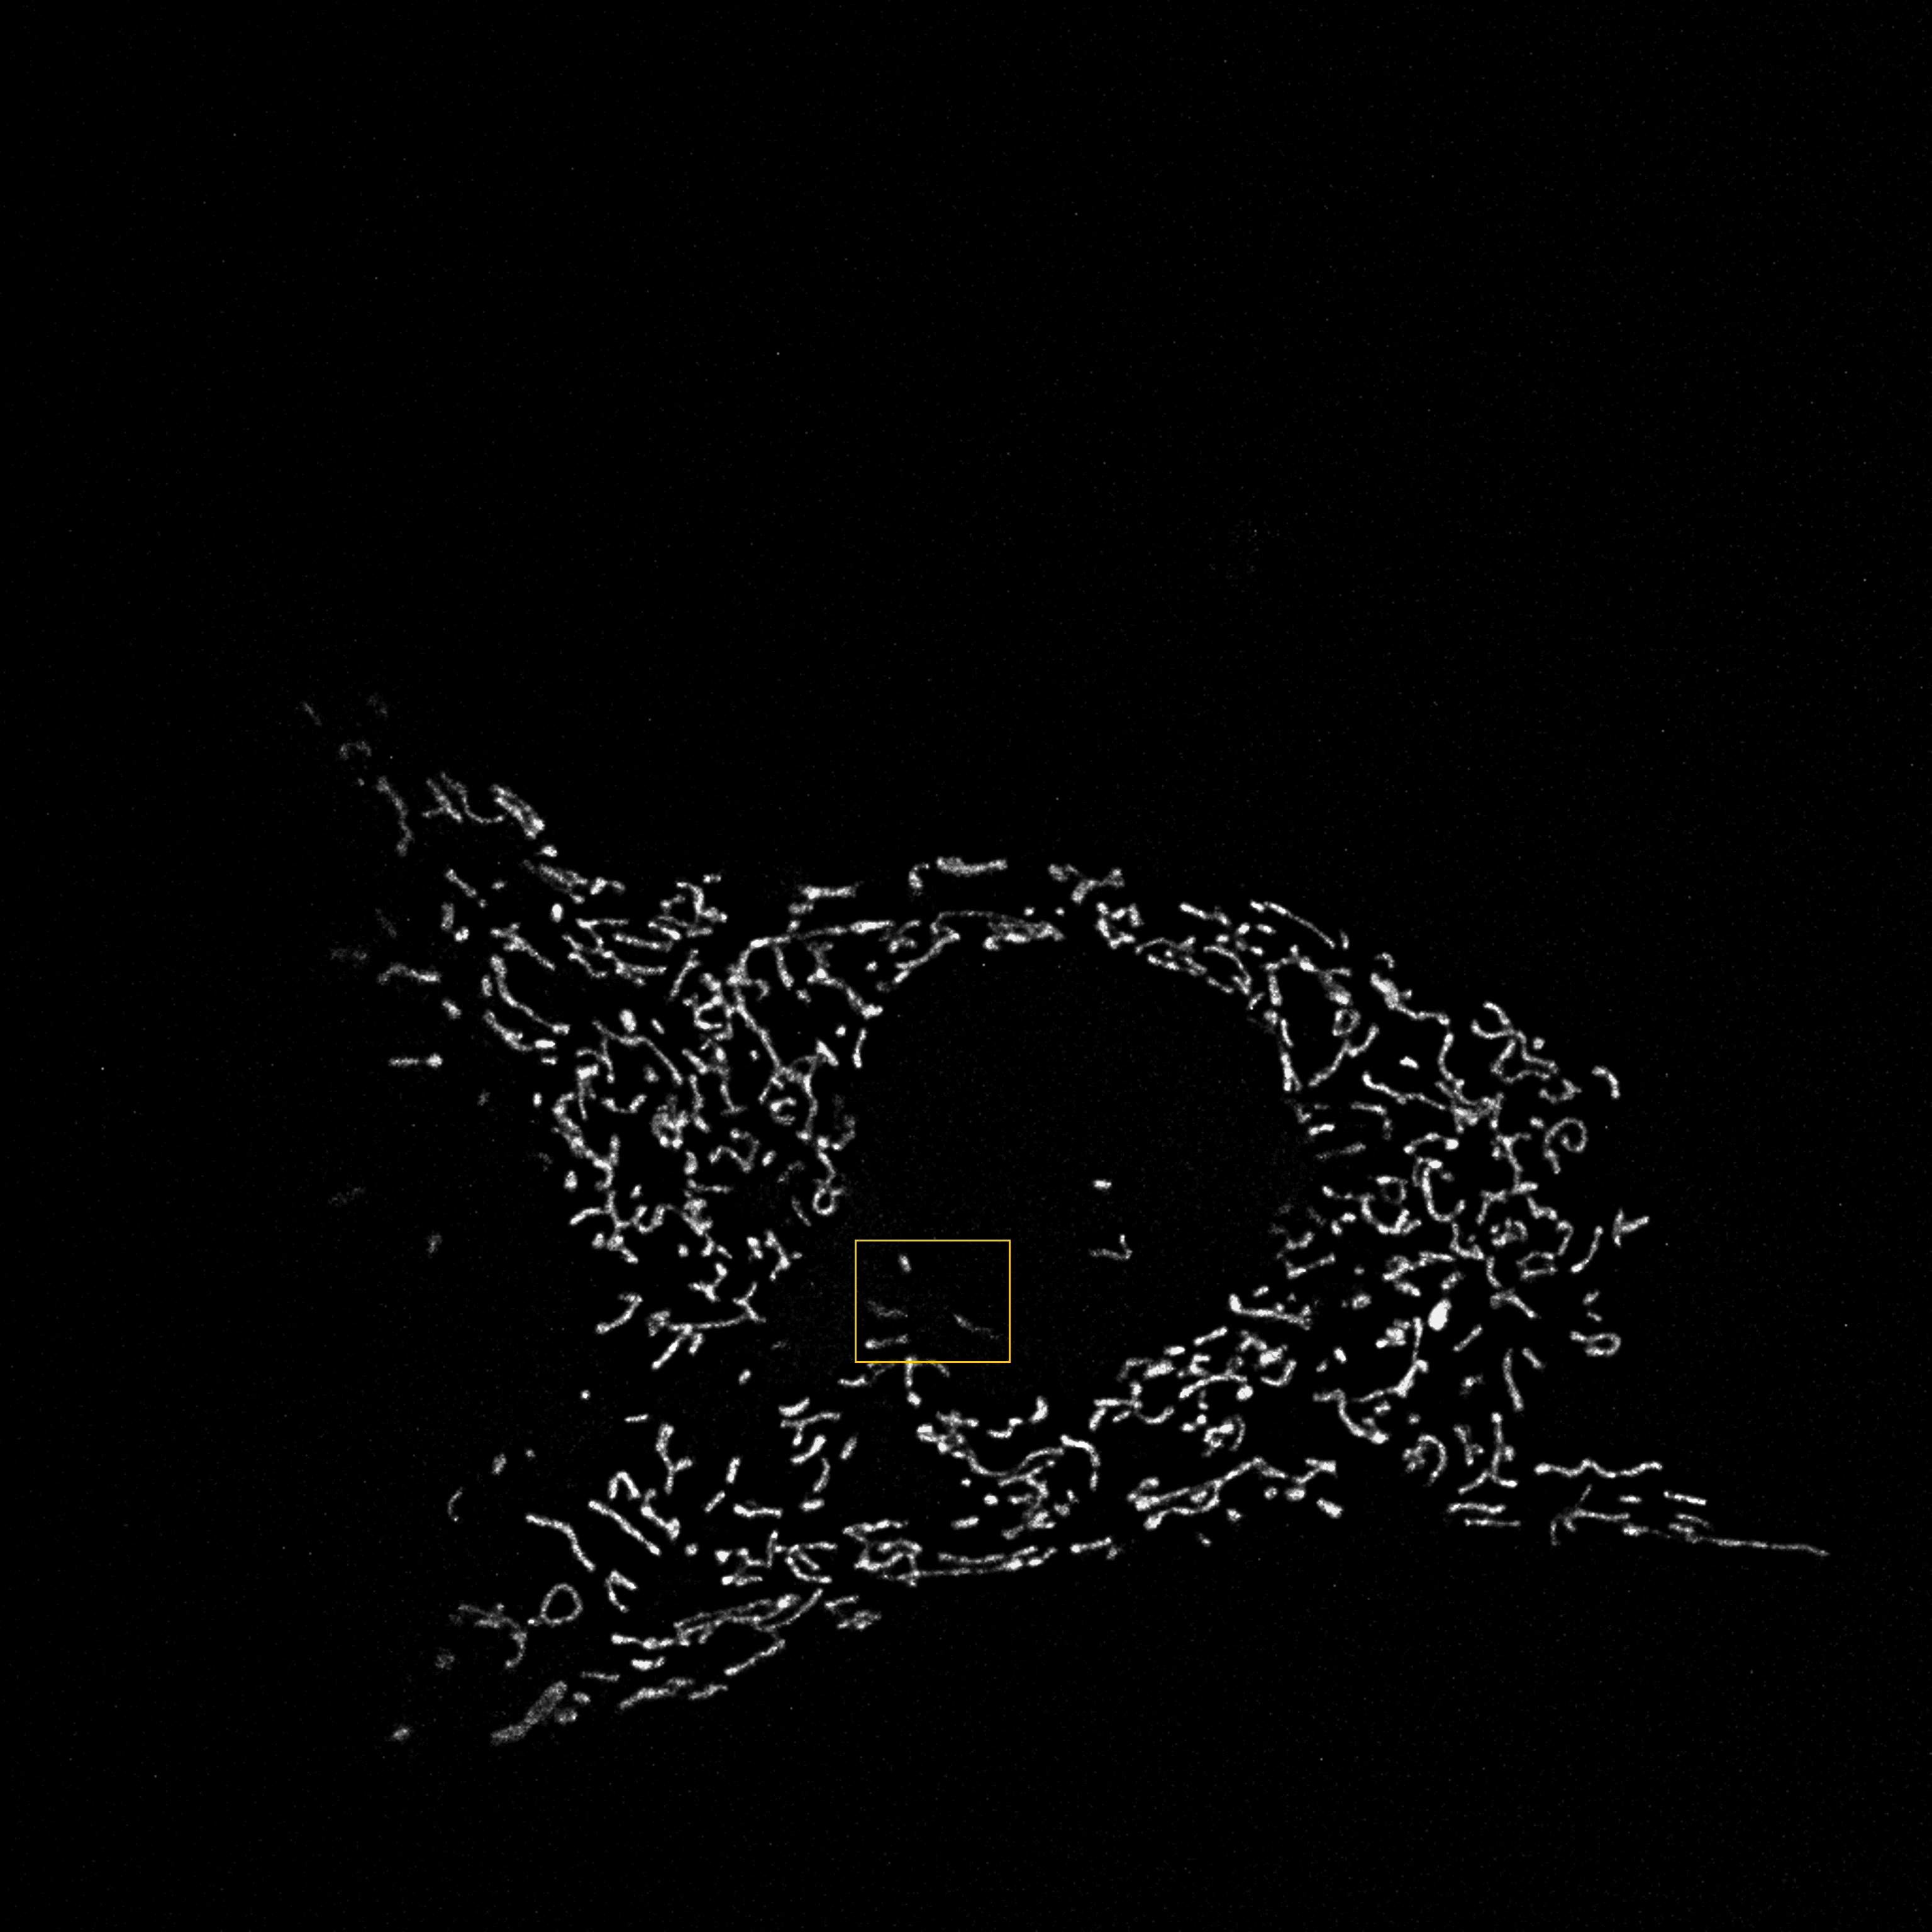
\includegraphics[width=0.48\linewidth]{figs/ch2figs/MAX_N1CCCP_1C=1_background_subtract.png}
    }}
    \subcaptionbox{After denoising\label{subfig:after_denoise}}{
    \stackinset{r}{3pt}{t}{1pt}{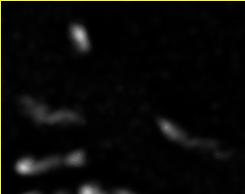
\includegraphics[width=0.15\linewidth, cframe=orange 0.5pt]{figs/ch2figs/Cropped_after_sigma.png}}{
    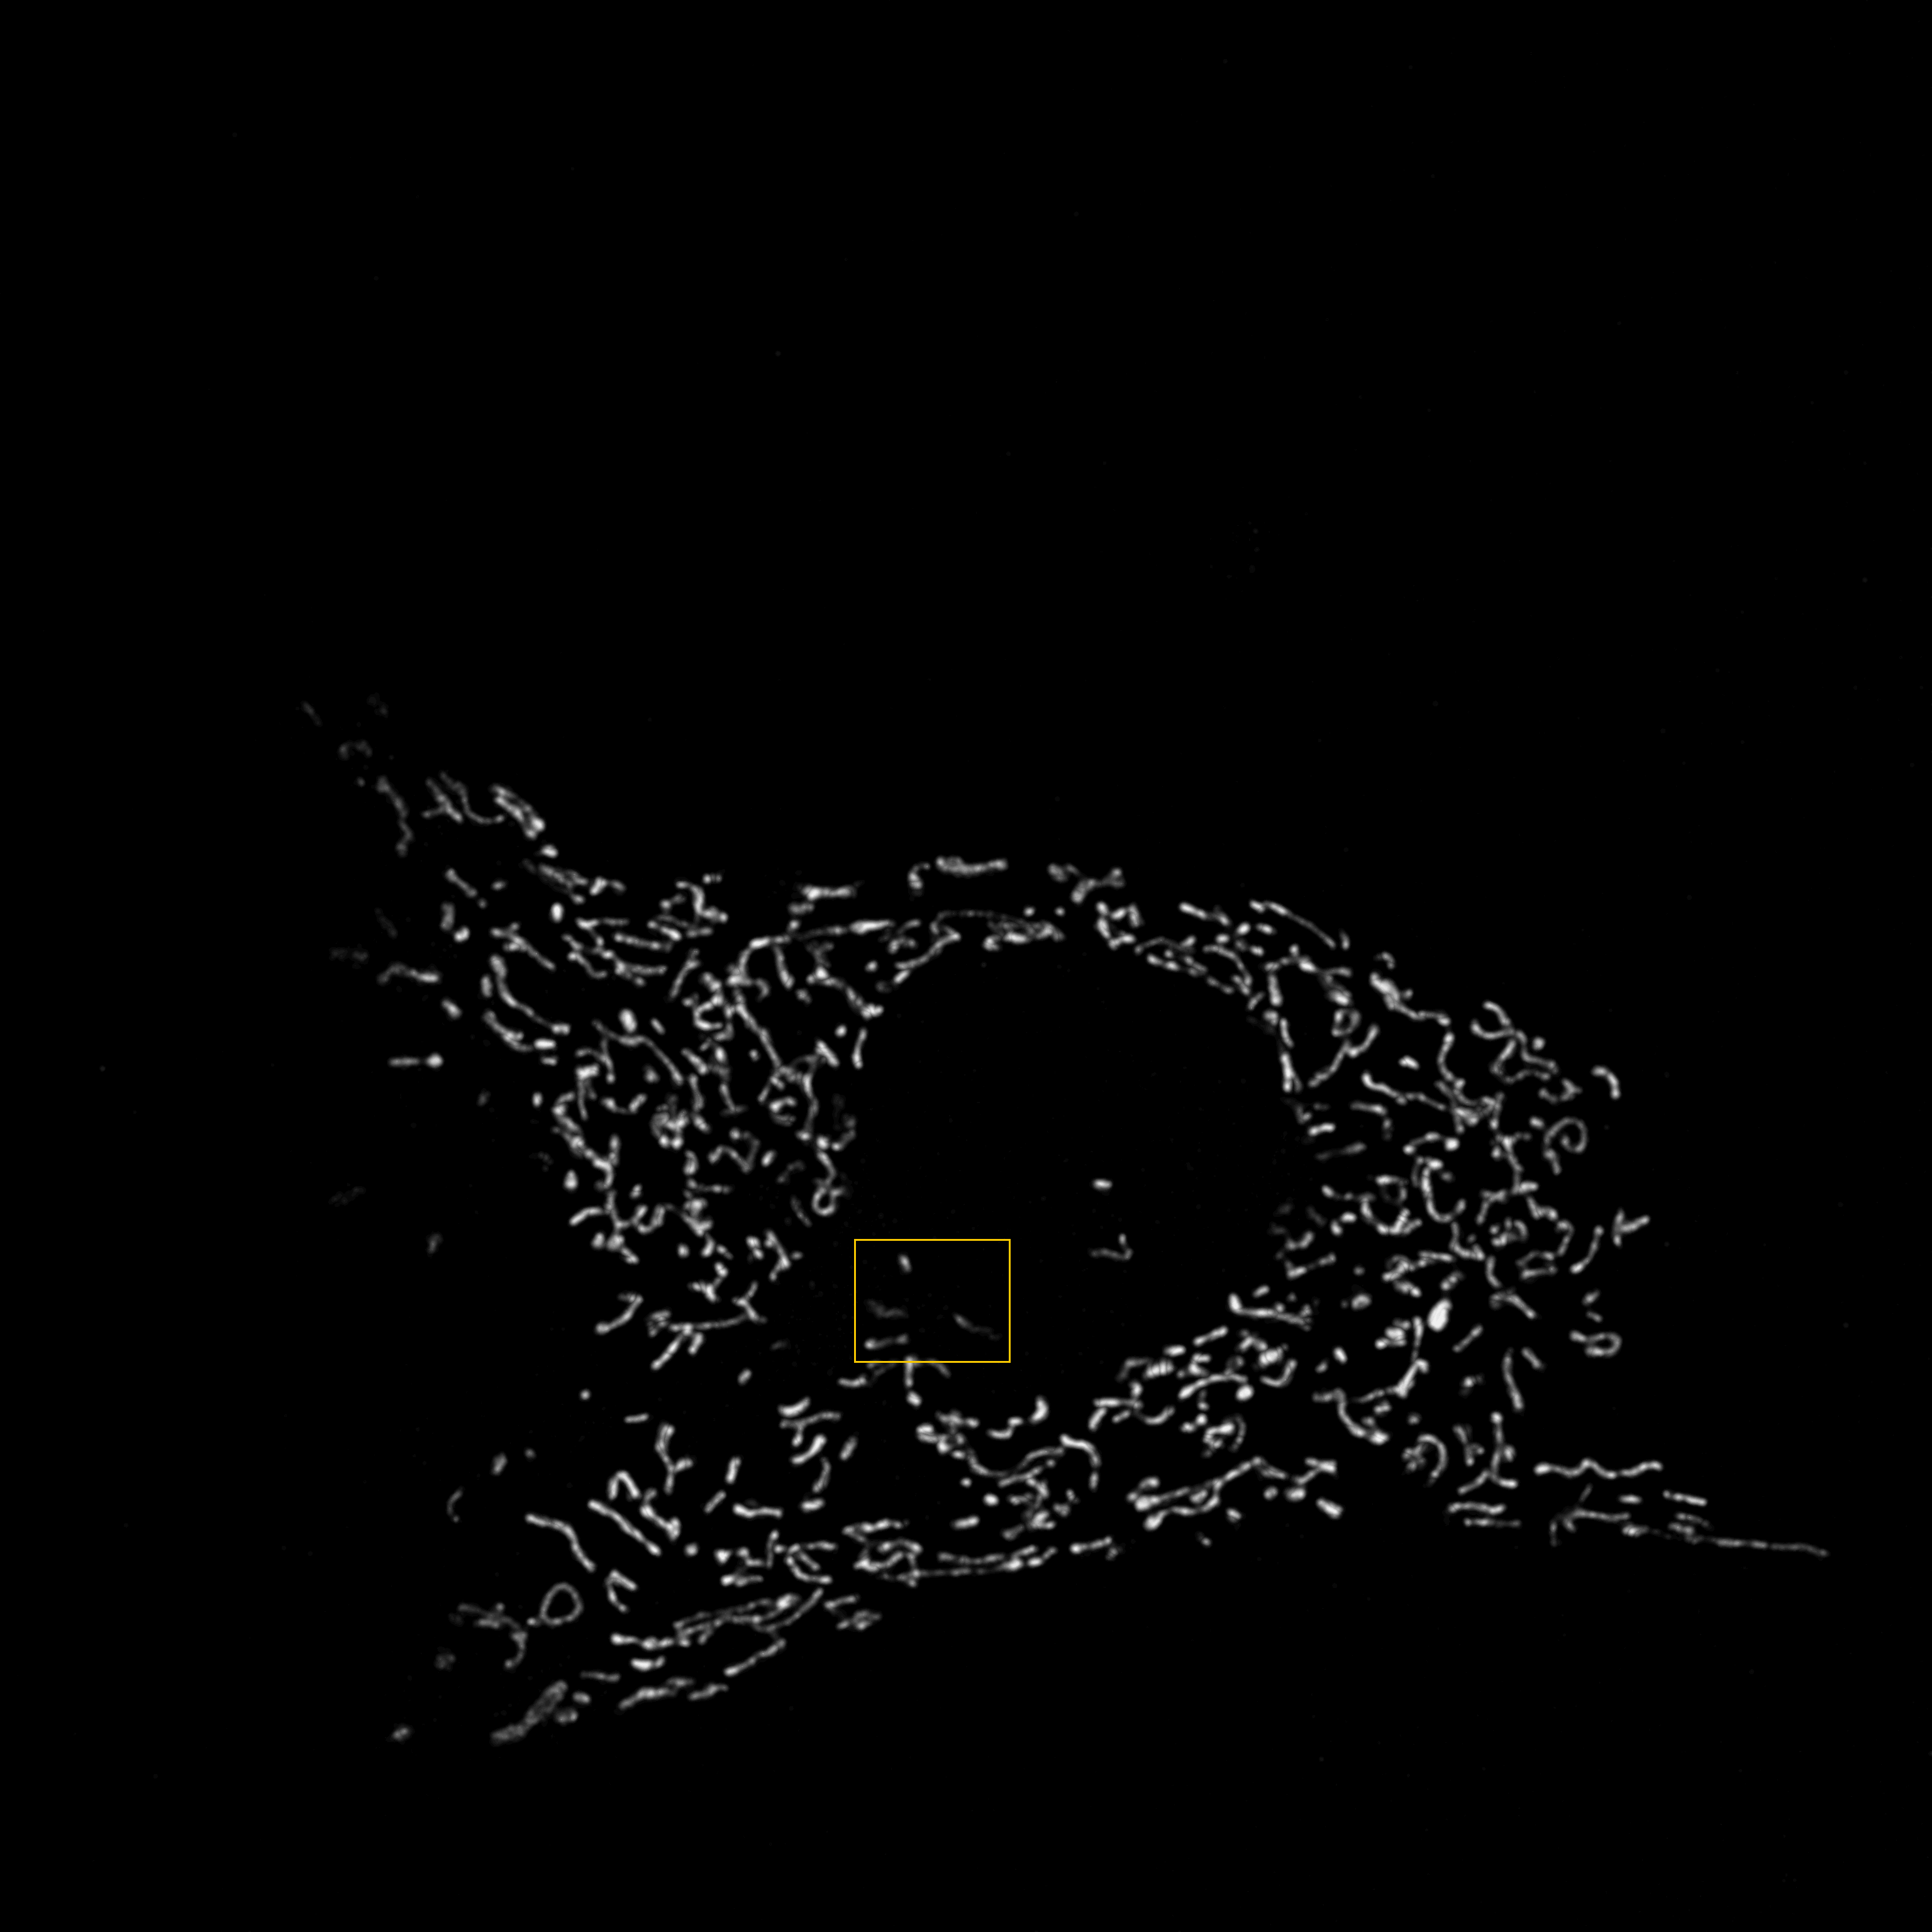
\includegraphics[width=0.48\linewidth]{figs/ch2figs/MAX_N1CCCP_1C=1_sigma_filter.png}}}
    \caption[Visual showcase of the effect of filtering on a maximum intensity projection image]{The effect of filtering on a mitochondria sample with before (\subref{subfig:before_denoise}) and after (\subref{subfig:after_denoise}). The sample images are maximum-intensity projects flattened from 3D with a region of interest bordered with an orange frame with a zoom-in at the top-right}
    \label{fig:denoising_example}
\end{figure}

\subsubsection{Image Enhancement}
While denoising methods are optimal for removing consistently present random fluctuations in pixel intensity across the image they are not designed to improve image signal strength or correct uneven signal distributions throughout the image which do not describe image features such as object edges and the region of pixels composing the body of the object. Object bodies are typically composed of pixels within a bounded range (excluding outliers) with the lower bound being of a magnitude greater than the background with the brighter pixels closer to the object centre or clustered around it. What is important is that image enhancement is easier to characterise by two components: firstly, the goal of it is to amplify the presence of both objects in the image and features describing said objects, like edges, and, secondly, while all image enhancement methods aim to enhance the image how this is done less consistent than other method types as it improved clarity and differentiation of objects from the background.\par
Before exploring the behaviour of image enhancement techniques the clarity and differentiation regarding image objects will be detailed for this context. Image objects have a body, described prior, surrounded by an edge which is in contrast to the pixels surrounding it whether those belong to some other object or the background. The contrast of the object edges is crucial to determine the boundaries of objects particularly when there are overlapping objects as insufficient contrast may lead to objects being incorrectly joined. The object body contrast does not need to be as large as the edges but must still contrast with the background as background regions in the object body could be cavities. For this reason, object differentiation is dependent on the size of the gap between the brightness of pixels composing the object and those composing the background while, in this context, the clarity is dependent on the brightness resolution of the image which can be viewed as the minimum and maximum pixel values of the image excluding outliers (outer values with relatively few pixels attributed to them) as a lower brightness resolution provides a more limited range within which to separate the object and background pixels. This also requires the background to be consistent as it is supposed to be the lowest brightness level in the image as it describes pixels where no fluorescence was localised in the actual specimen. These methods can range from contrast stretching to correcting uneven illumination. Contrast stretching can target either the whole image or localised regions within which to enhance the contrast present which is beneficial for contrast-dependent features such as detecting the edges of objects. 
Uneven illumination across the image is characterized by changes in the brightness of the pixels across the image that do not describe any objects as object edges or bodies. This change can appear to be homogeneous relative to the object sizes and interfere with the contrast required for differentiation. Due to this, methods correcting uneven illumination attempt to normalize the brightness of regions based on how low the variance within that region is i.e. brightness is lowered for homogeneous regions with low contrast while high contrast regions remain.\textcolor{red}{I struggled a bit with describing the correction of uneven illumination. While I feel my idea of it is correct the explanation feels a bit difficult. If you have any advice for simplifying it or what should be corrected in the explanation would be appreciated.} An example of correcting uneven illumination across the background is the rolling ball algorithm~\cite{rolling_ball} while an example of contrast enhancement is seen in ``Contrast limited adaptive histogram equalization''(CLAHE)~\cite{clahe}.

\begin{figure}
    \centering
    \subcaptionbox{Intensity image of the specimen prior to CLAHE\label{subfig:middleslice_noclahe}}{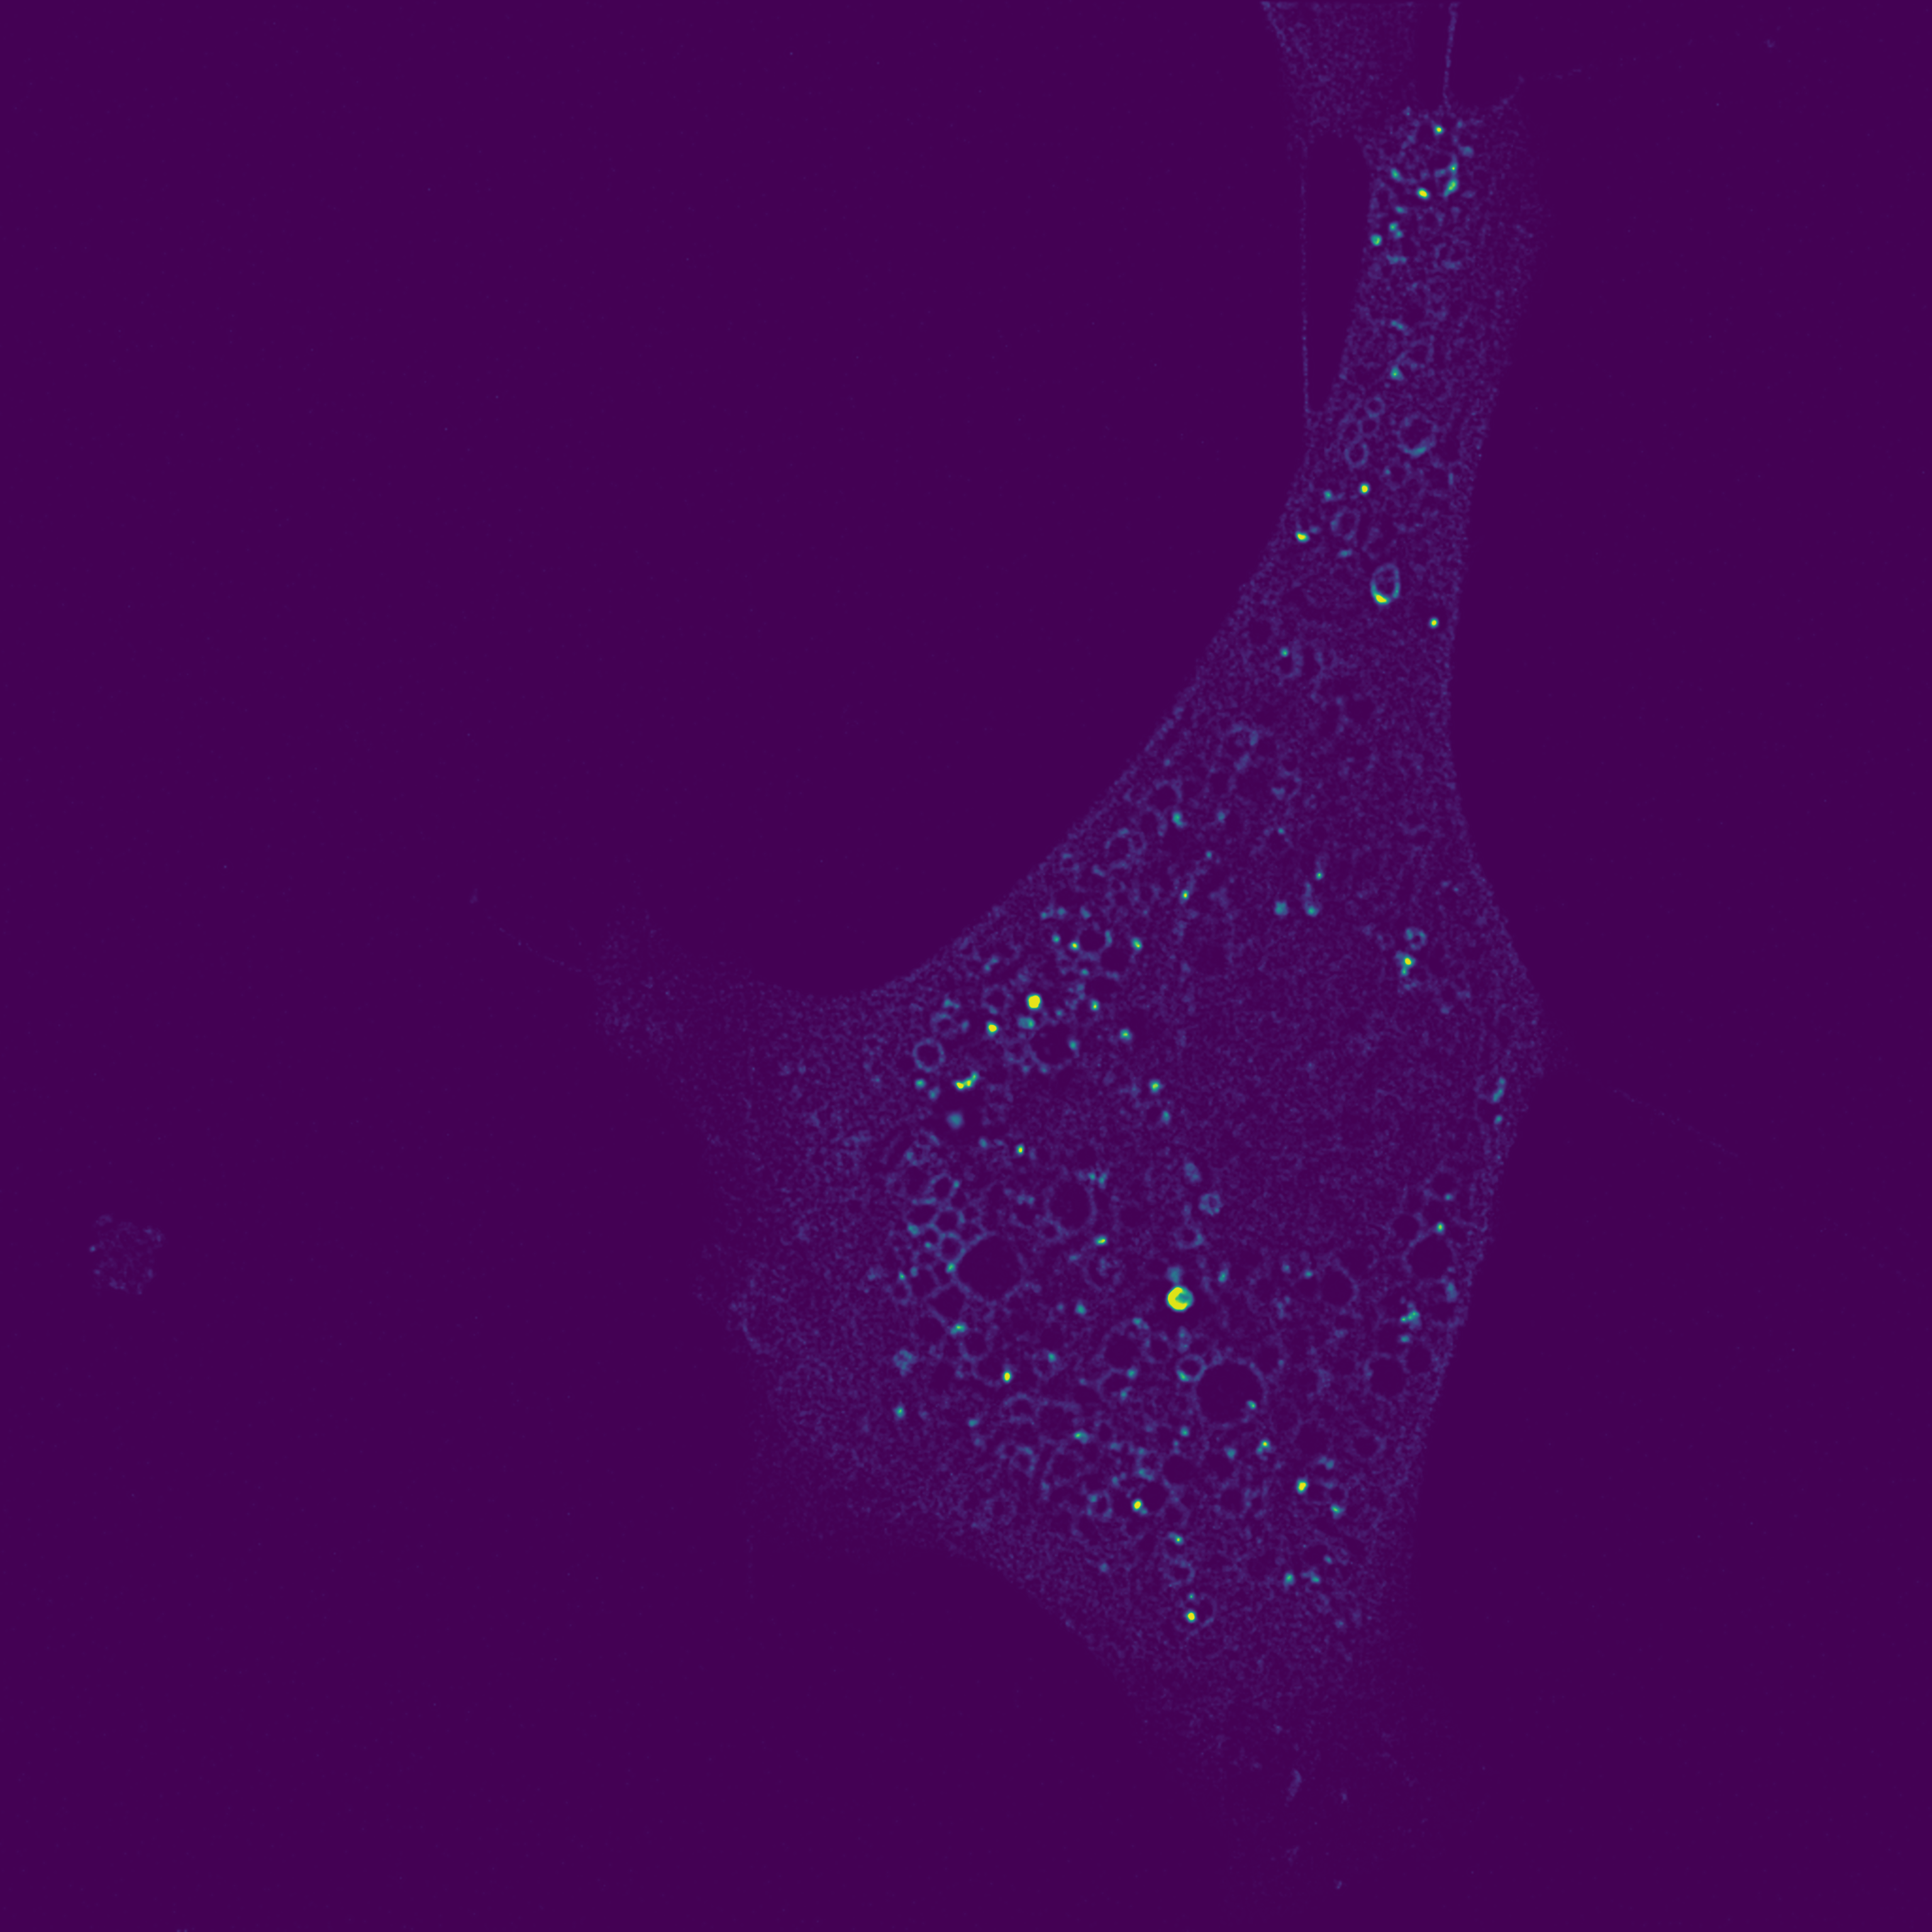
\includegraphics[width=0.49\linewidth]{figs/ch2figs/N2Con_3C=0T=0_middleslice_bs.png}}
    \subcaptionbox{Intensity image of the specimen after CLAHE\label{subfig:middleslice_clahe}}{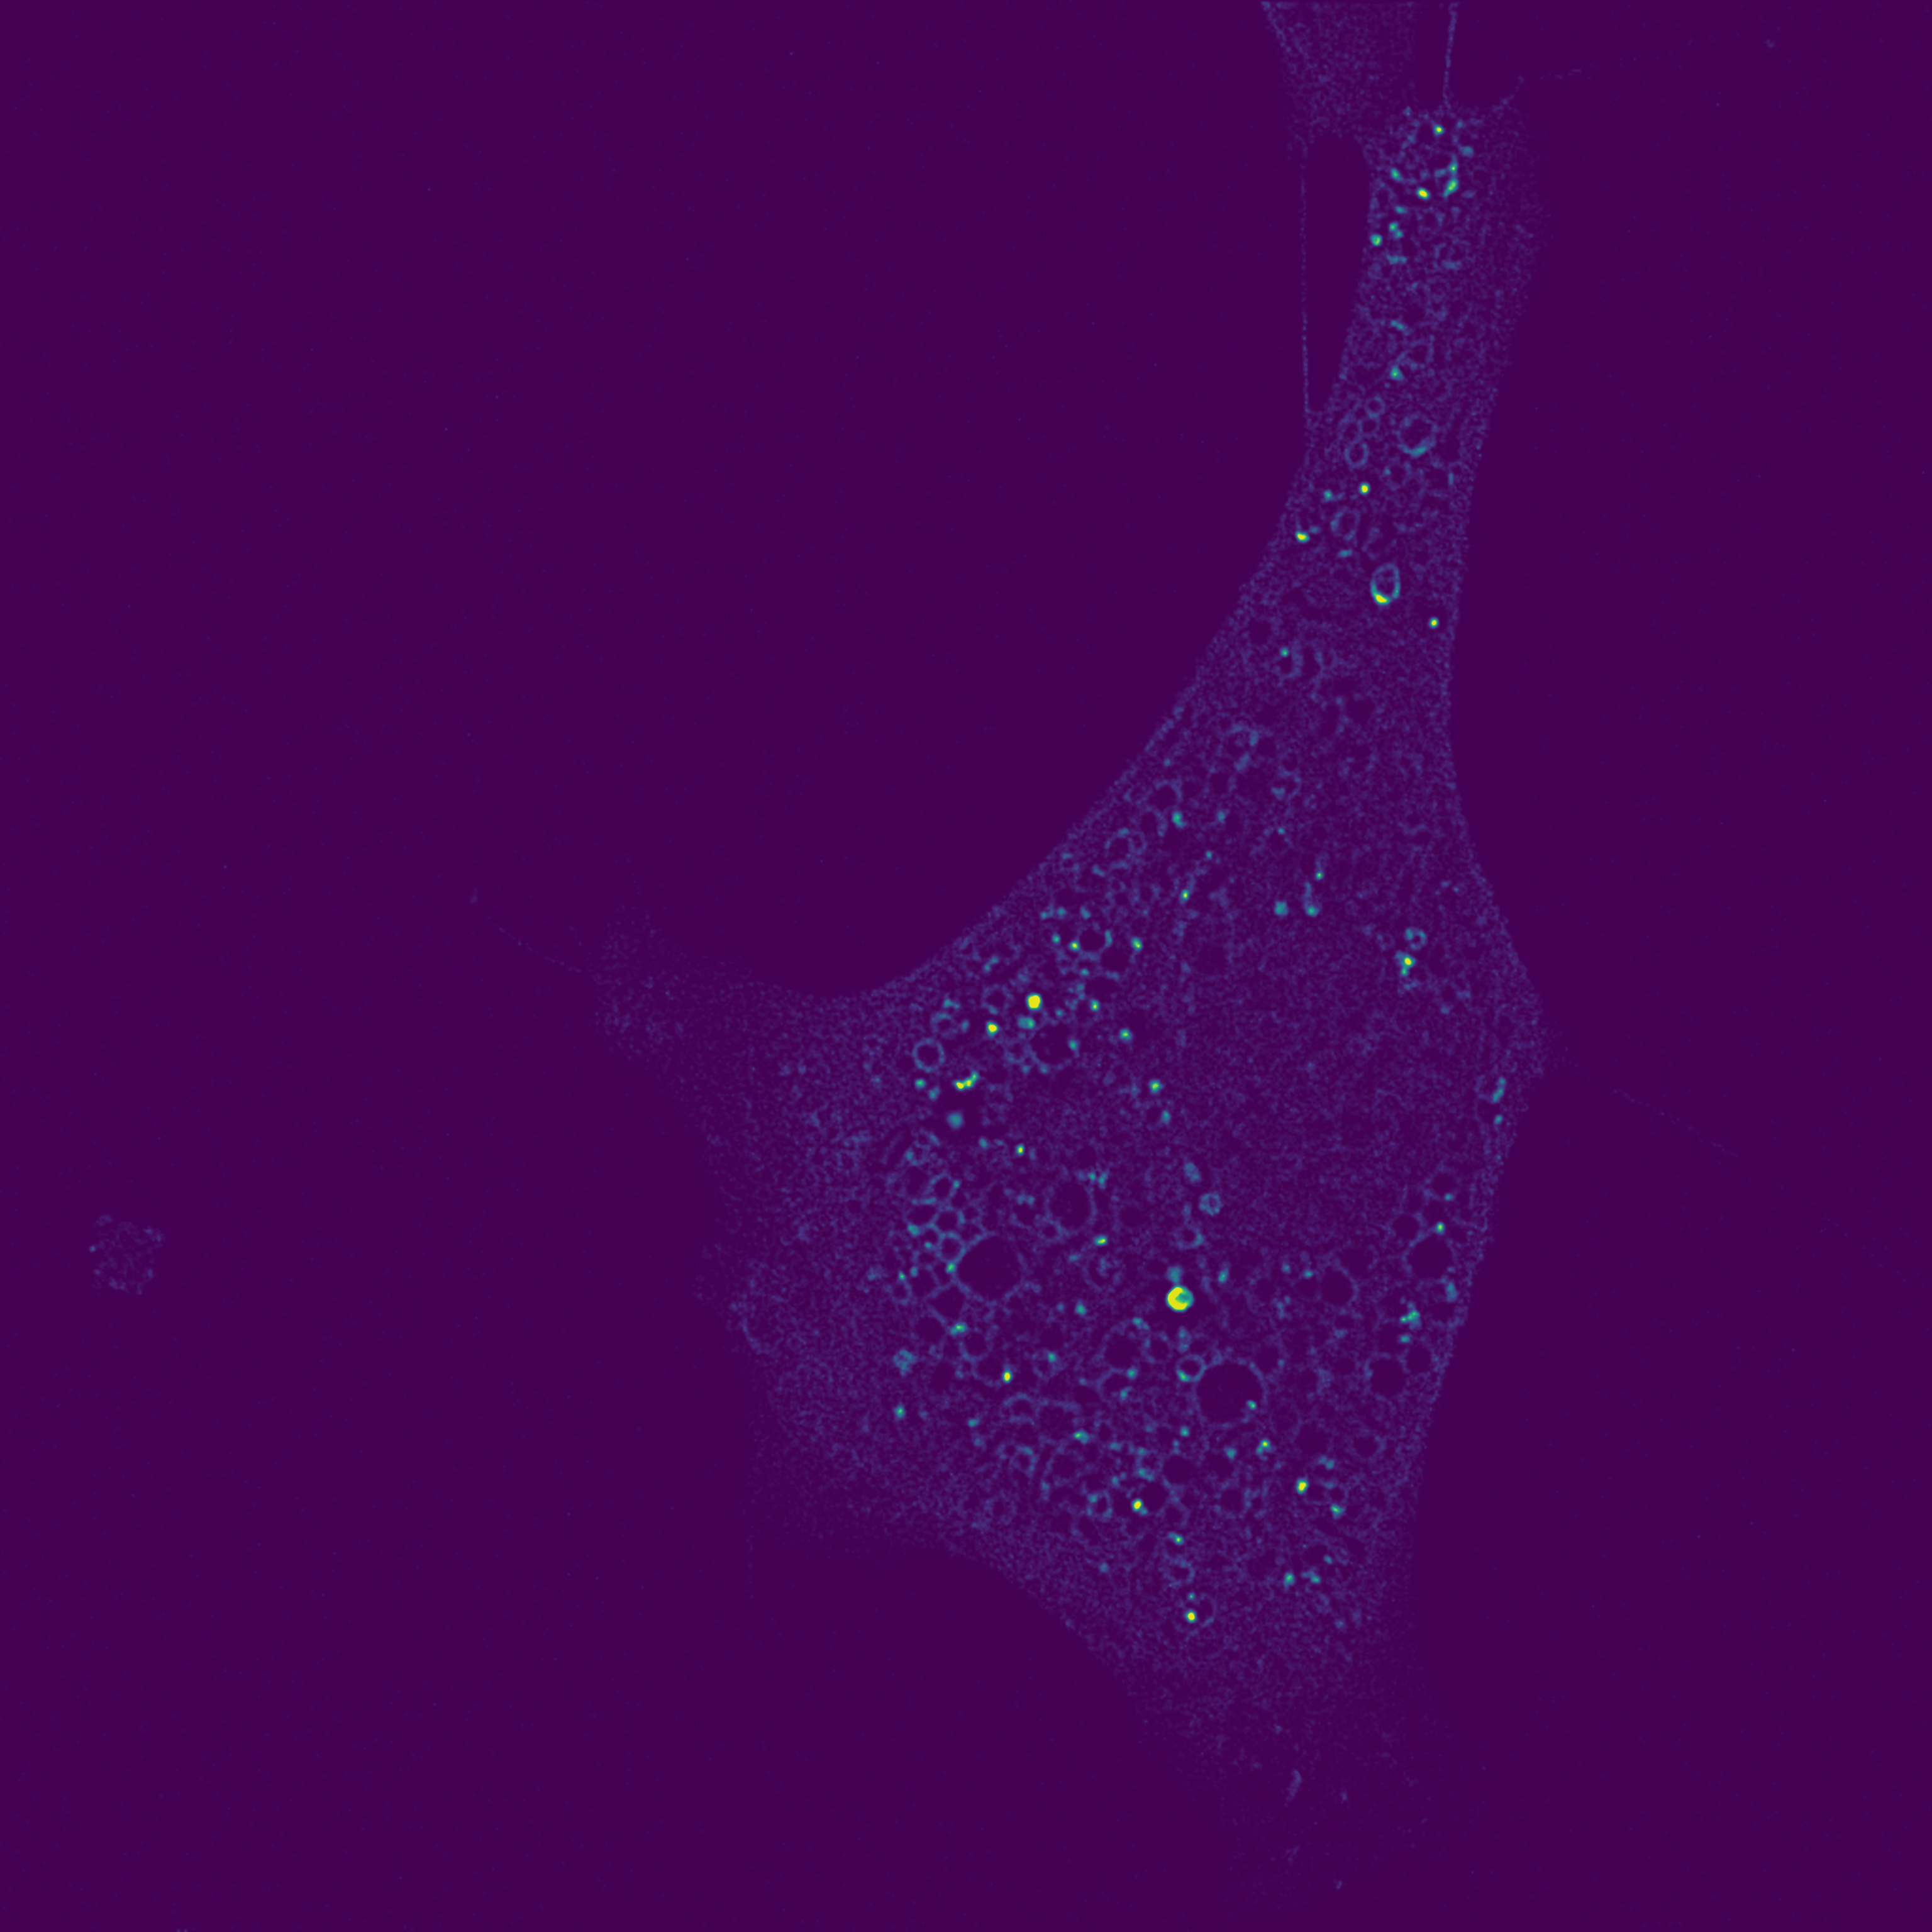
\includegraphics[width=0.49\linewidth]{figs/ch2figs/N2Con_3C=0T=0_middleslice_clahe.png}}
    \subcaptionbox{Binarised image after the Otsu threshold has been applied to Image \subref{subfig:middleslice_noclahe})\label{subfig:otsu_before_clahe}}{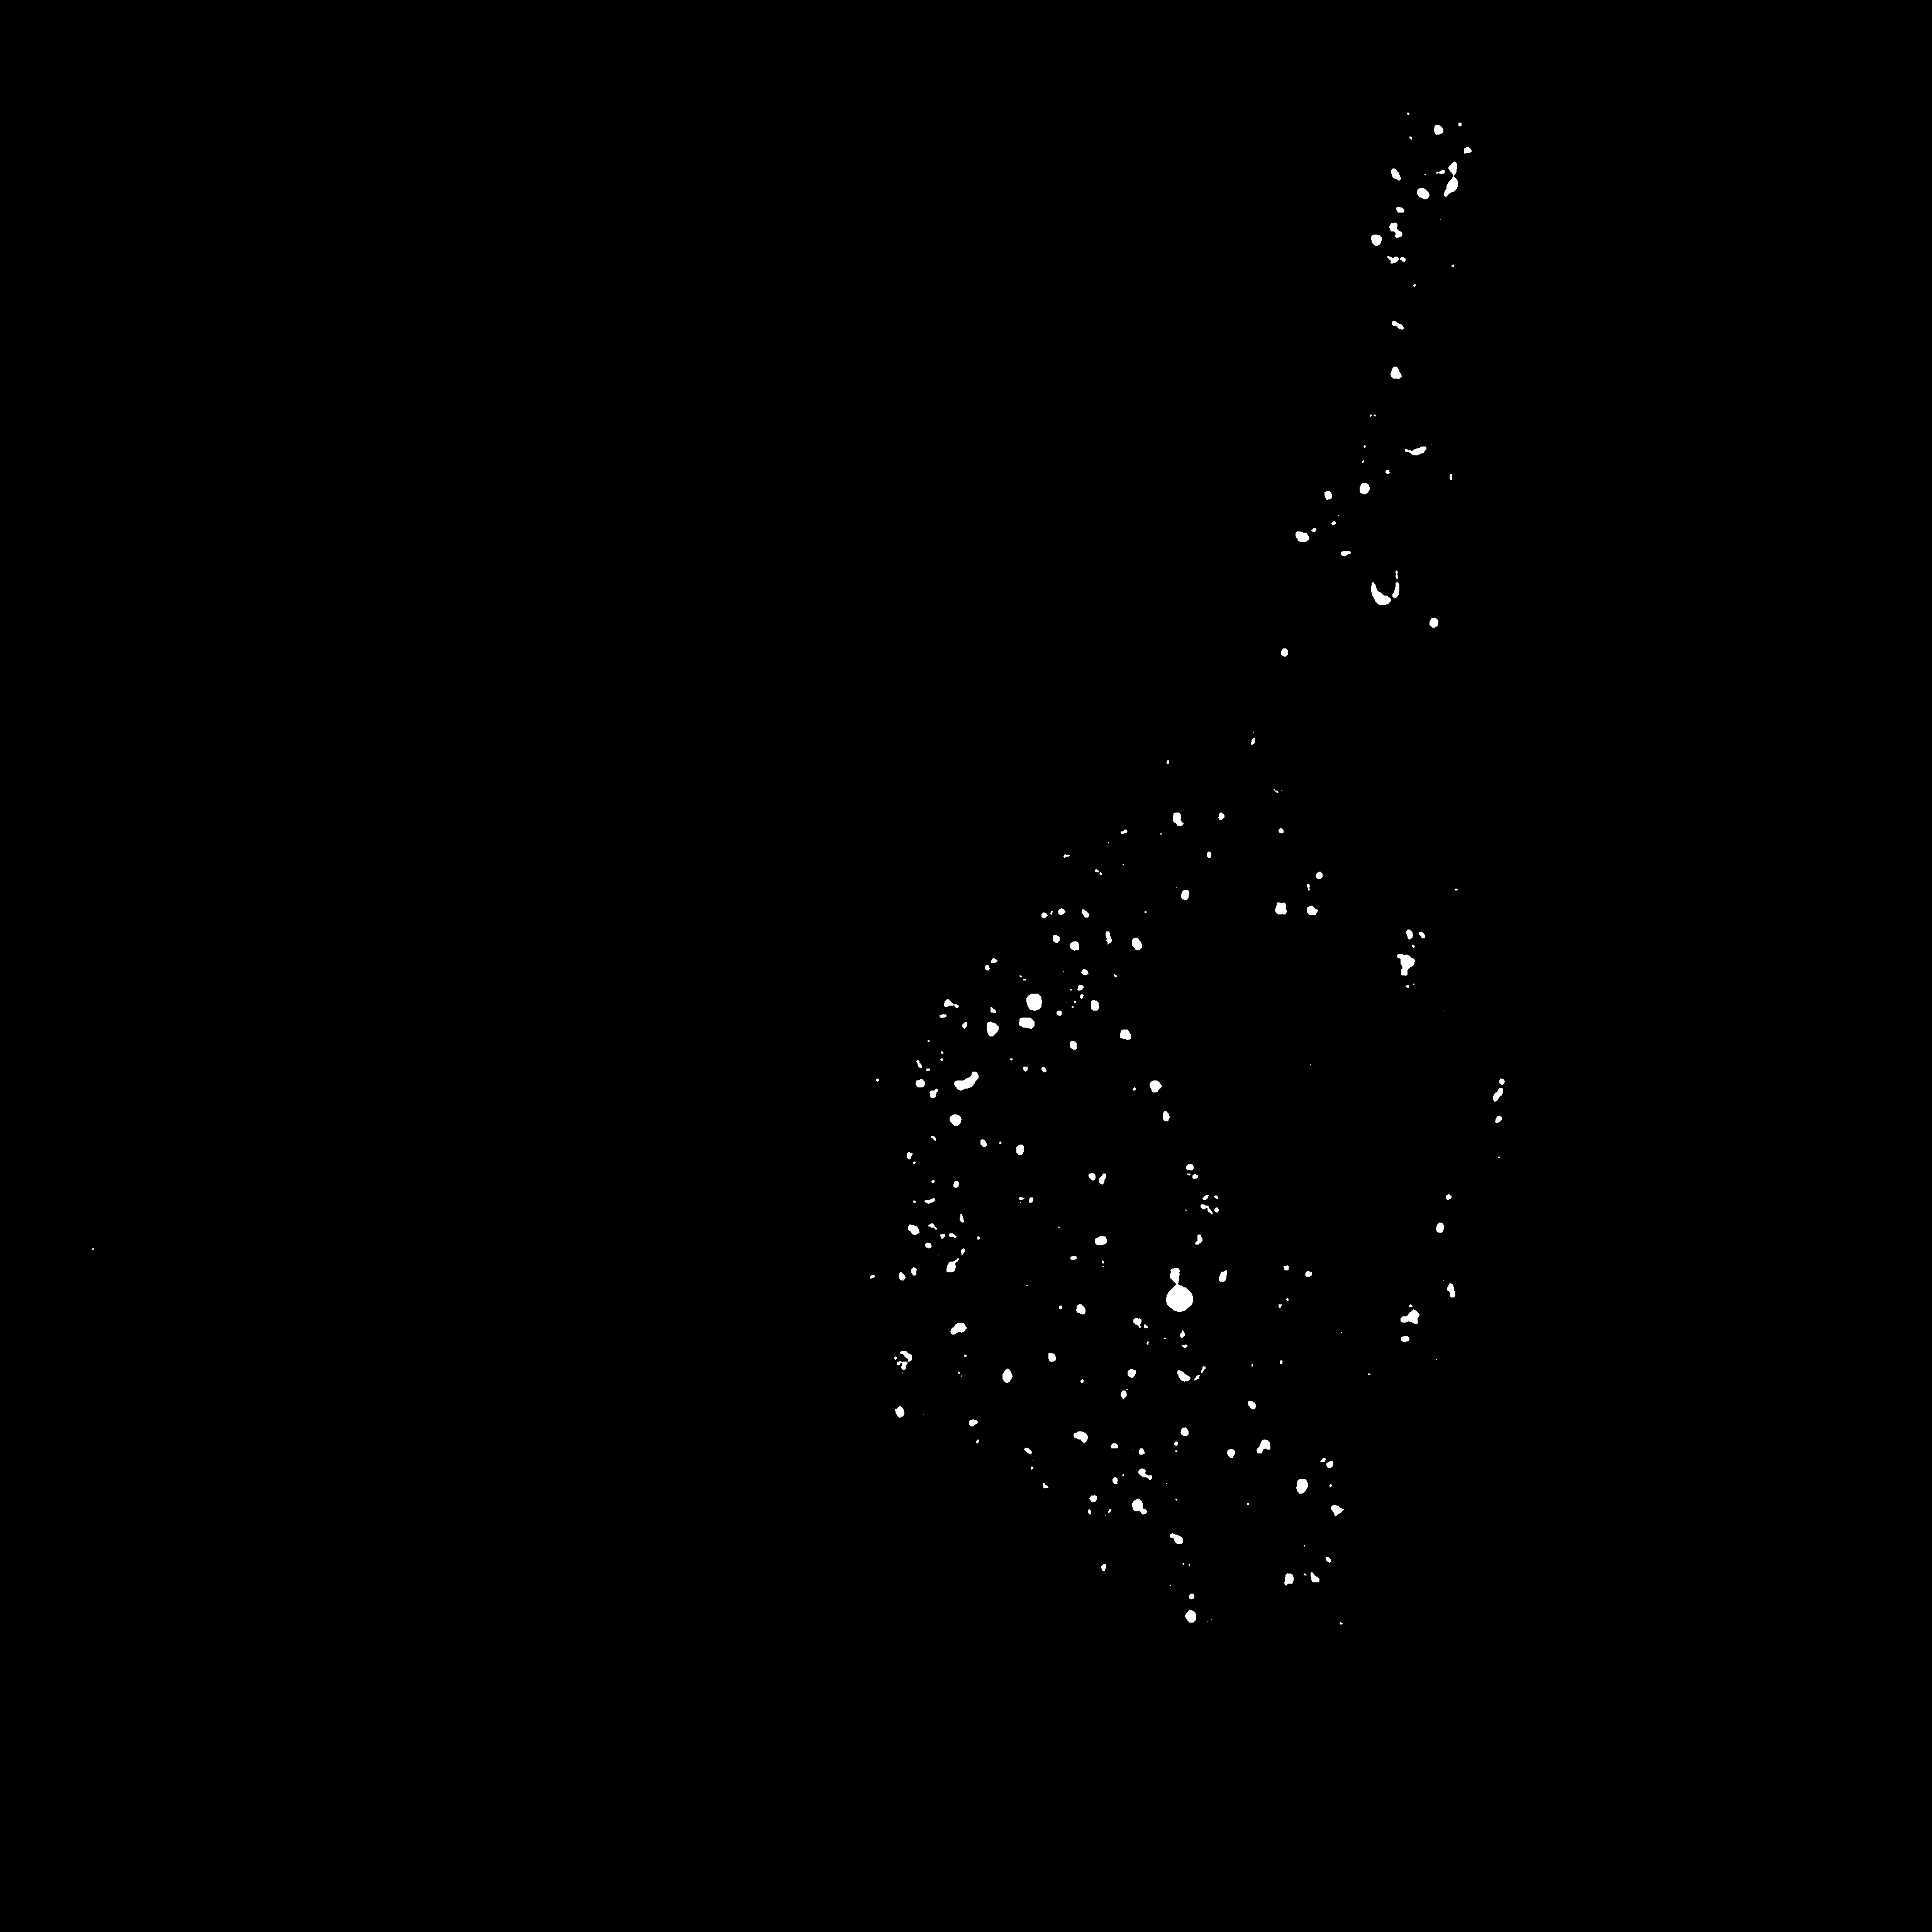
\includegraphics[width=0.49\linewidth]{figs/ch2figs/N2Con_3C=0T=0_noclahe_otsu.png}}
    \subcaptionbox{Binarised image after the Otsu threshold has been to image \subref{subfig:middleslice_clahe})\label{subfig:clahe_otsu_applied}}{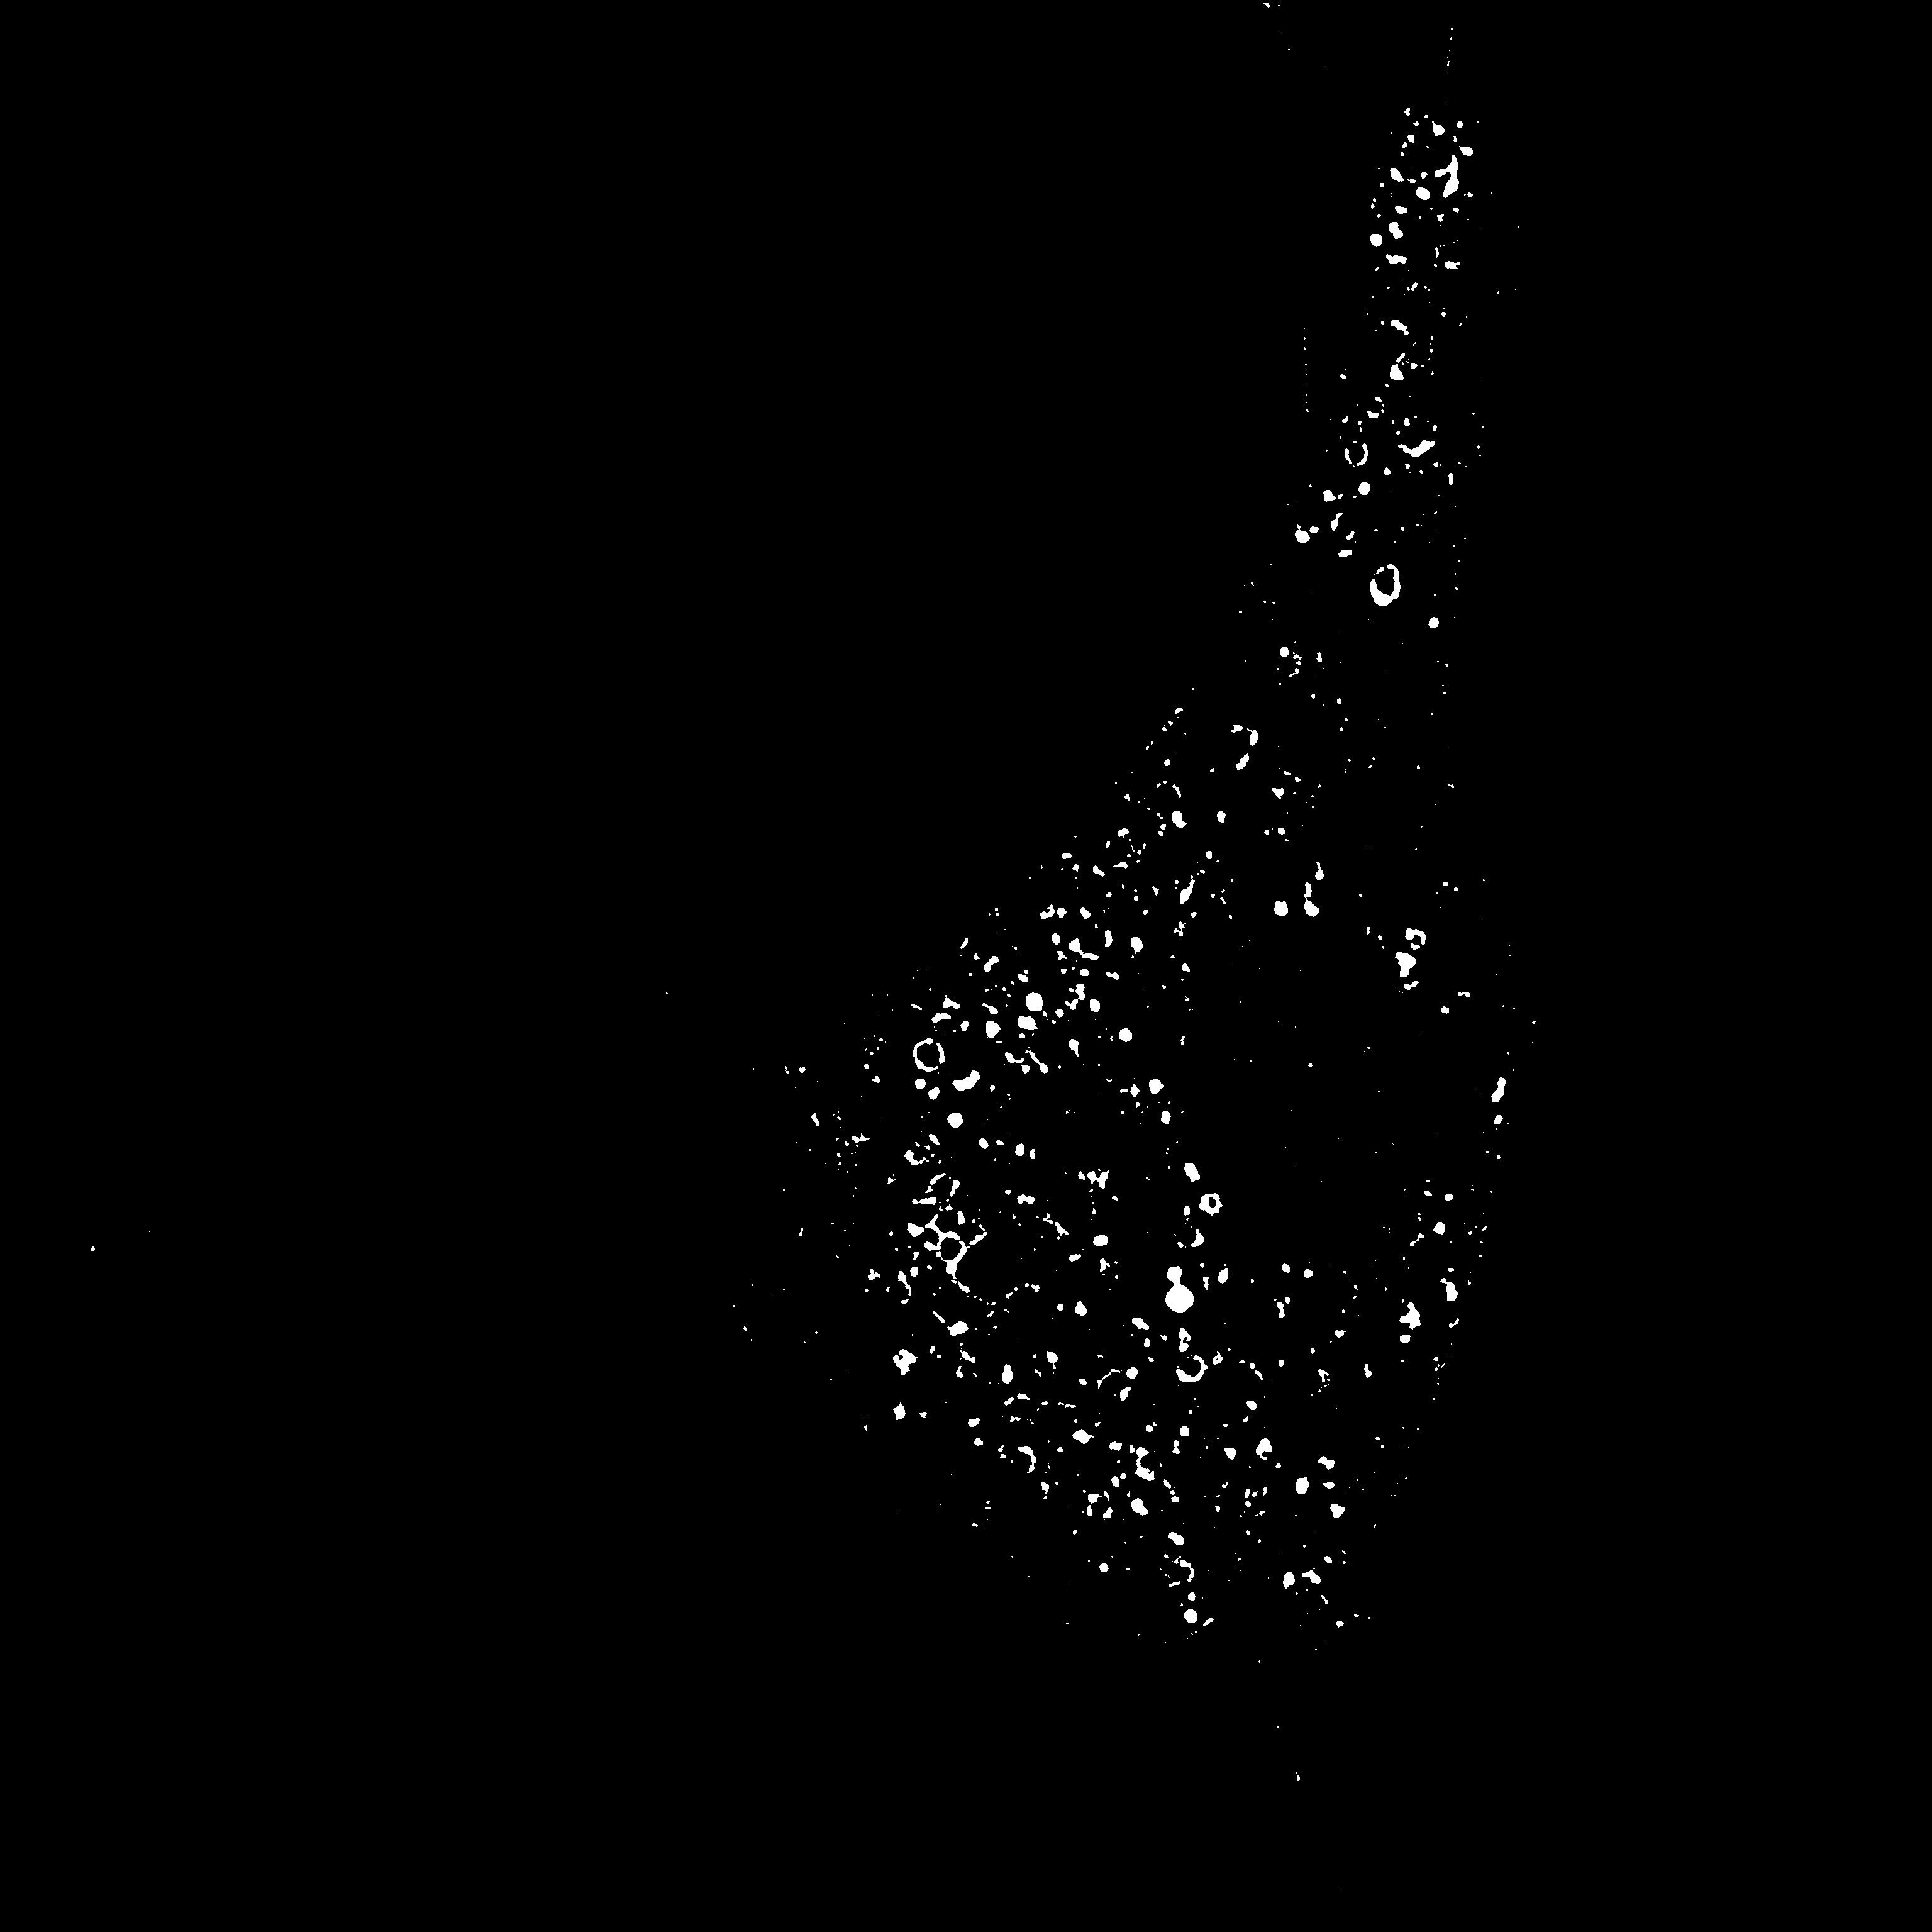
\includegraphics[width=0.49\linewidth]{figs/ch2figs/N2Con_3C=0T=0_clahe_otsu.png}}
    
    \caption[Visual showcase of the effect of contrast enhancement on image thresholding]{The impact of contrast enhancement on the image analysis process is presented regarding the automated thresholding between foreground and background structures. The specimen image is shown in (\subref{subfig:middleslice_noclahe}) which has had background subtraction applied and CLAHE has been applied to this image to restore contrast as shown in (\subref{subfig:middleslice_clahe}). The impact of this on global thresholding (Otsu) is shown in (\subref{subfig:otsu_before_clahe}) which is Otsu applied before CLAHE and (\subref{subfig:clahe_otsu_applied}) is the result of Otsu after CLAHE has been applied.}
\end{figure}
\par
\textcolor{red}{For the background subtraction, I have been struggling to find images to which I can apply background subtraction myself (that actually have uneven illumination). Do you think it is fine if I use this image from scikit-image? \textit{https://scikit-image.org/docs/stable/\_images/\\sphx\_glr\_plot\_rolling\_ball\_001.png}}
\subsubsection{Thresholding}\label{subsec:thresholding}
Thresholding is a method by which pixels are assigned a label dependent on the pixel value in relation to a threshold value (lesser or greater than). In a pre-processing context, this is typically applied to differentiate between foreground and background pixels. This functions under the assumption that objects of interest in the image will be composed of pixels with a value greater than the threshold thus all objects of interest will be assigned to the foreground. Background pixels on the other hand are artefacts, noise or objects not of interest (appearing due to autofluorescence, out-of-focus fluorescence, or bleed-through). After threshold application, only the foreground pixels, those belonging to objects of interest, will be preserved.\par Outside of pre-processing threshold methods technically fall under image segmentation which is a body of techniques that assign labels to pixels based on some criteria. Image segmentation has a myriad of methods depending on the field of application (microscopy, morphological analysis, object detection, etc.) where the number of labels is determined by the number of groups that an object, described by pixels, can belong to. This application is relative to pre-processing thus the focus is on thresholding images to get binary classifications (foreground or background).\par With the binary classification of images to separate pixels composing objects of interest from `other' pixels (where `other' refers to noise, artefacts and inconsistent background illumination) a single threshold value is required to classify each pixel. This classifying behaviour is consistent across all threshold methods but the determination of the threshold value is what changes between methods. There are two groups of threshold methods which are global thresholding and local thresholding~\cite{segmentation_book} with the former determining a threshold using and applying it across the entire image while the latter determines and applies the thresholds across localised regions of the image.
\paragraph{Global thresholding}
Global methods, like \textit{Otsu thresholding}~\cite{Otsu1979ATS}, determine the threshold value using the image histogram by selecting an intensity value separating the histogram values into two groups. In ideal situations with a distinct separation between the grey-level intensities of the background and foreground will be characterized in the histogram with two peaks where the clusters centred around each peak correspond to the pixels for the foreground (higher intensity) and background (lower intensity) respectively~\cite[p.163]{segmentation_book}. An example of this can be seen in Figure \ref{fig:histogram_appearances} where the different potential histogram shapes are displayed.
\begin{figure}
    \centering
    \subcaptionbox{Bimodal histogram}{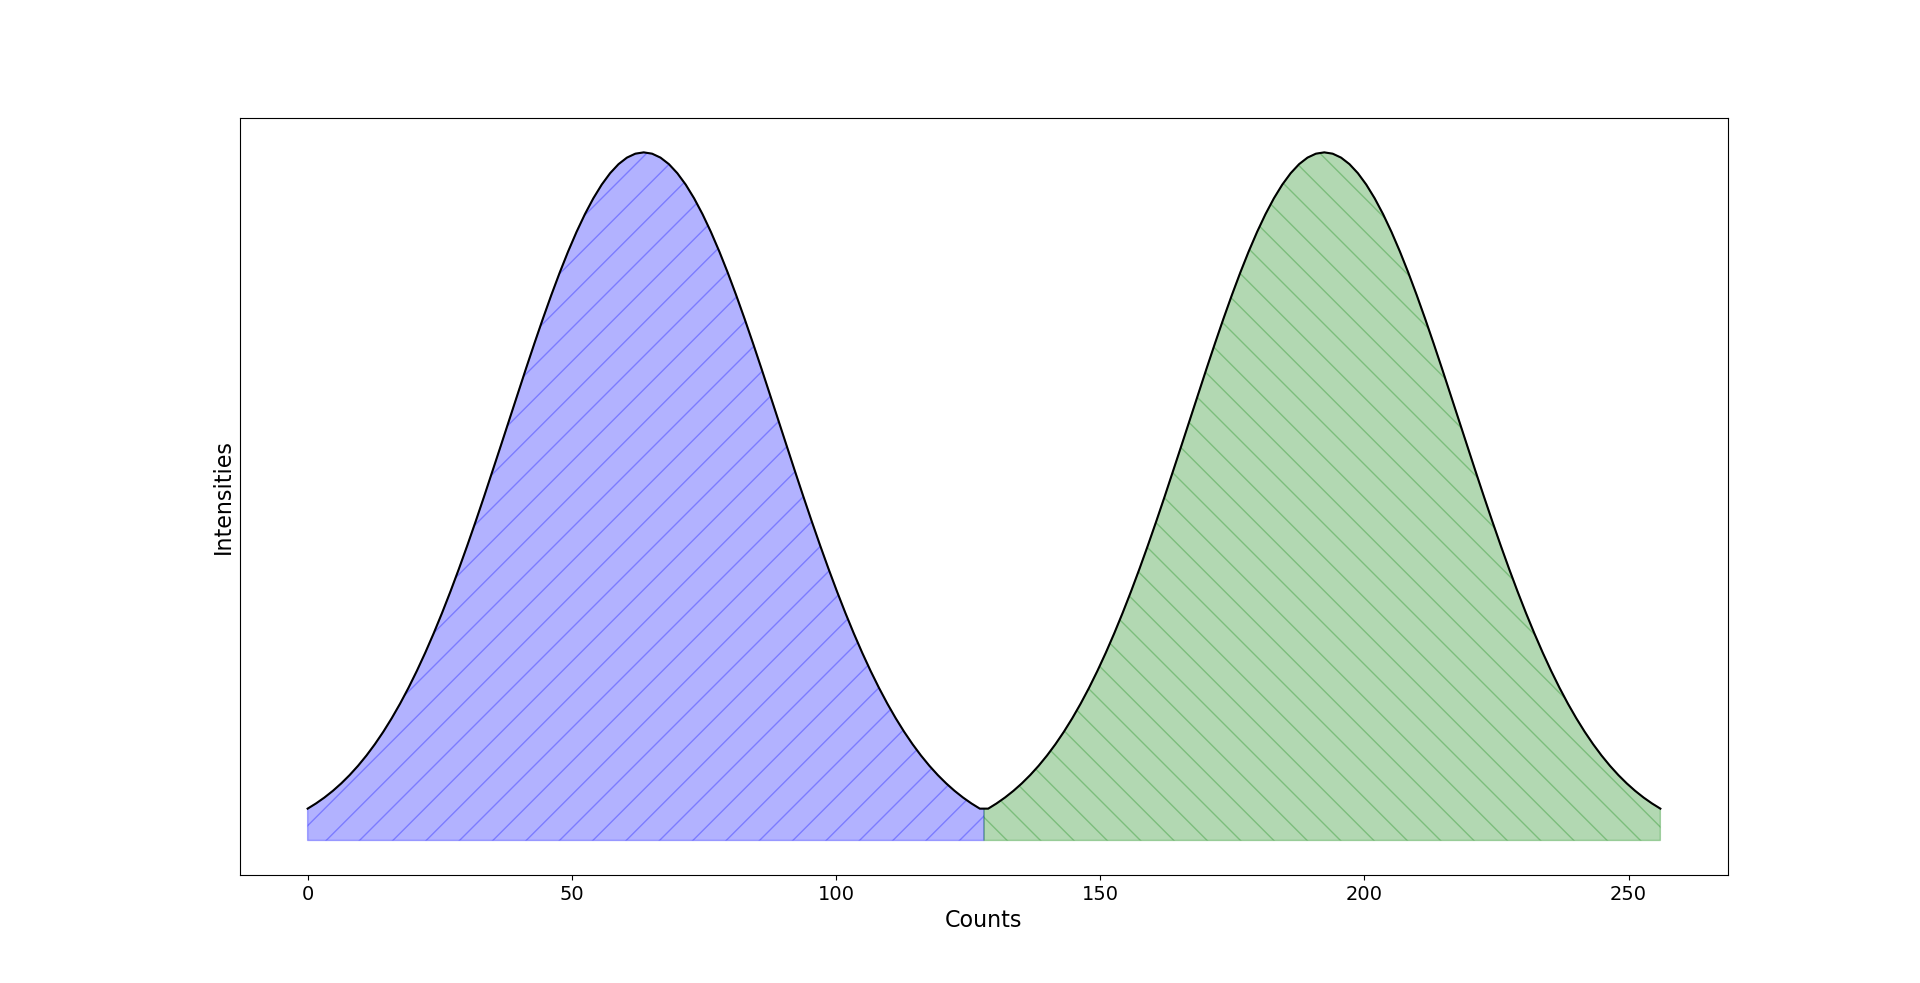
\includegraphics[width=0.32\linewidth]{figs/ch2figs/Bimodal.png}}
    \subcaptionbox{Unimodal histogram}{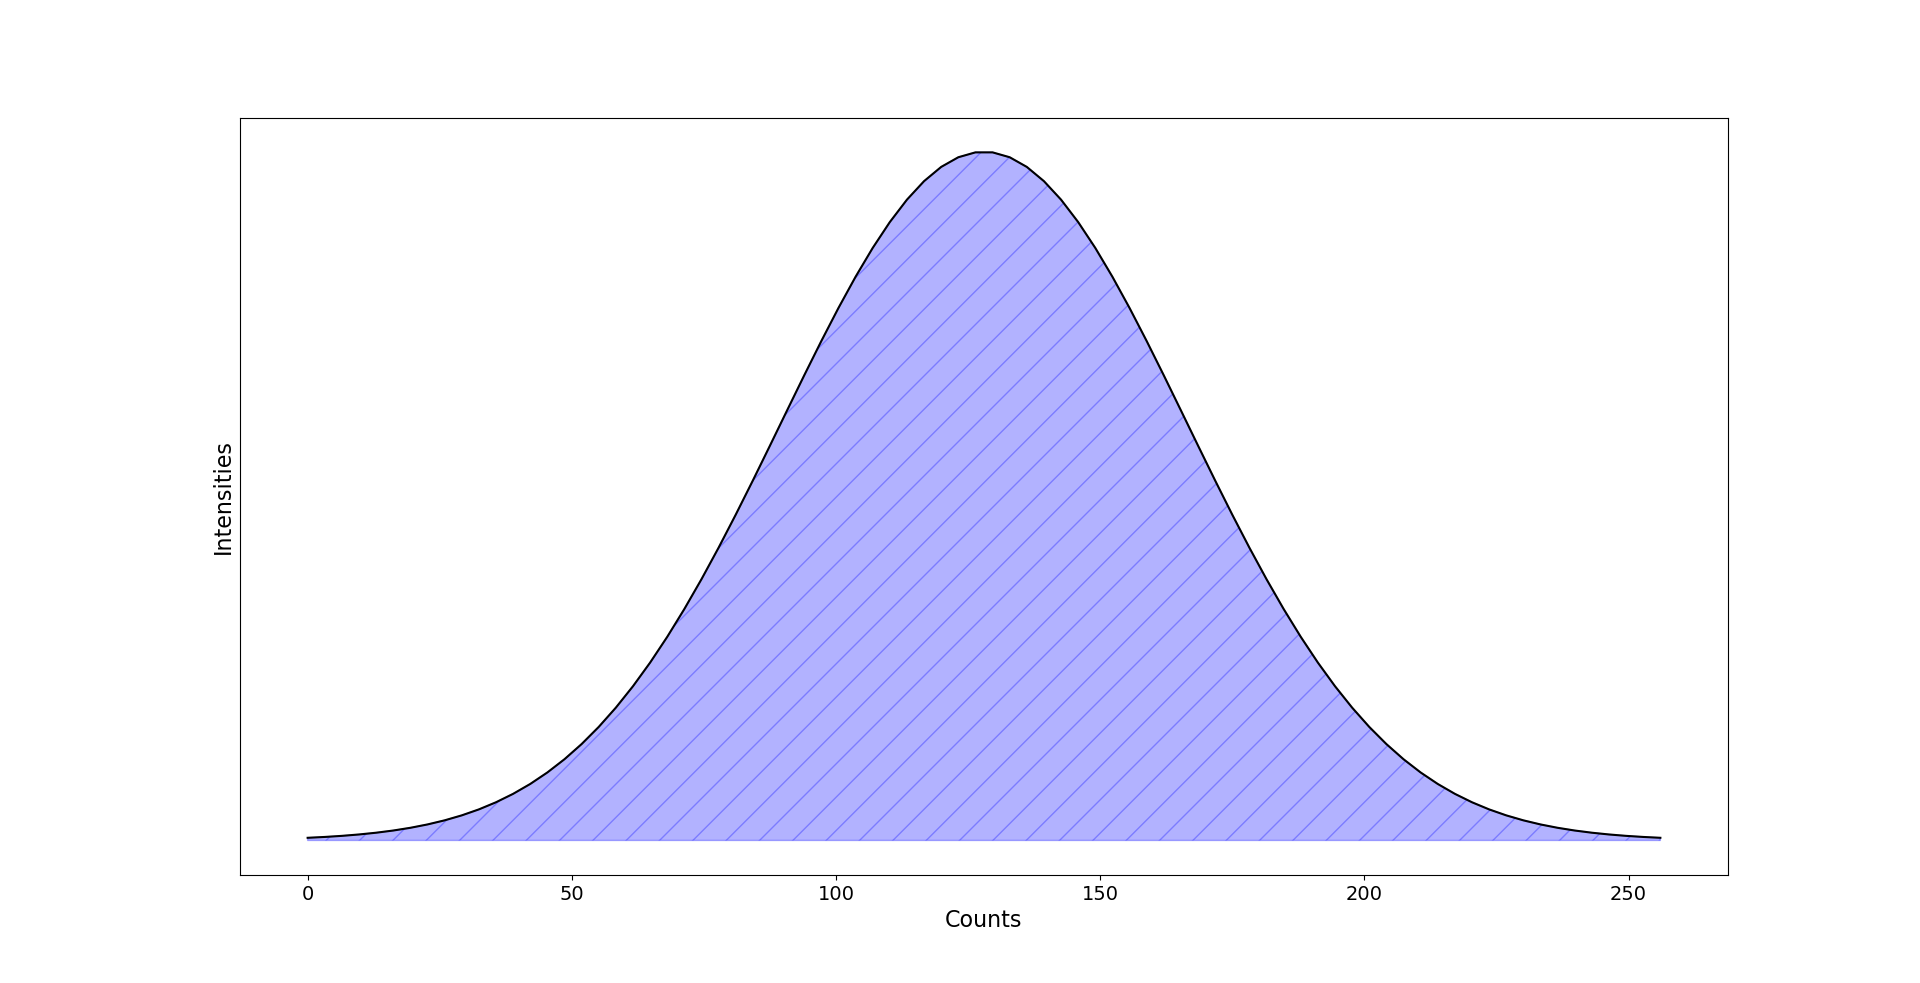
\includegraphics[width=0.32\linewidth]{figs/ch2figs/Unimodal.png}}
    \subcaptionbox{Dominant background histogram}{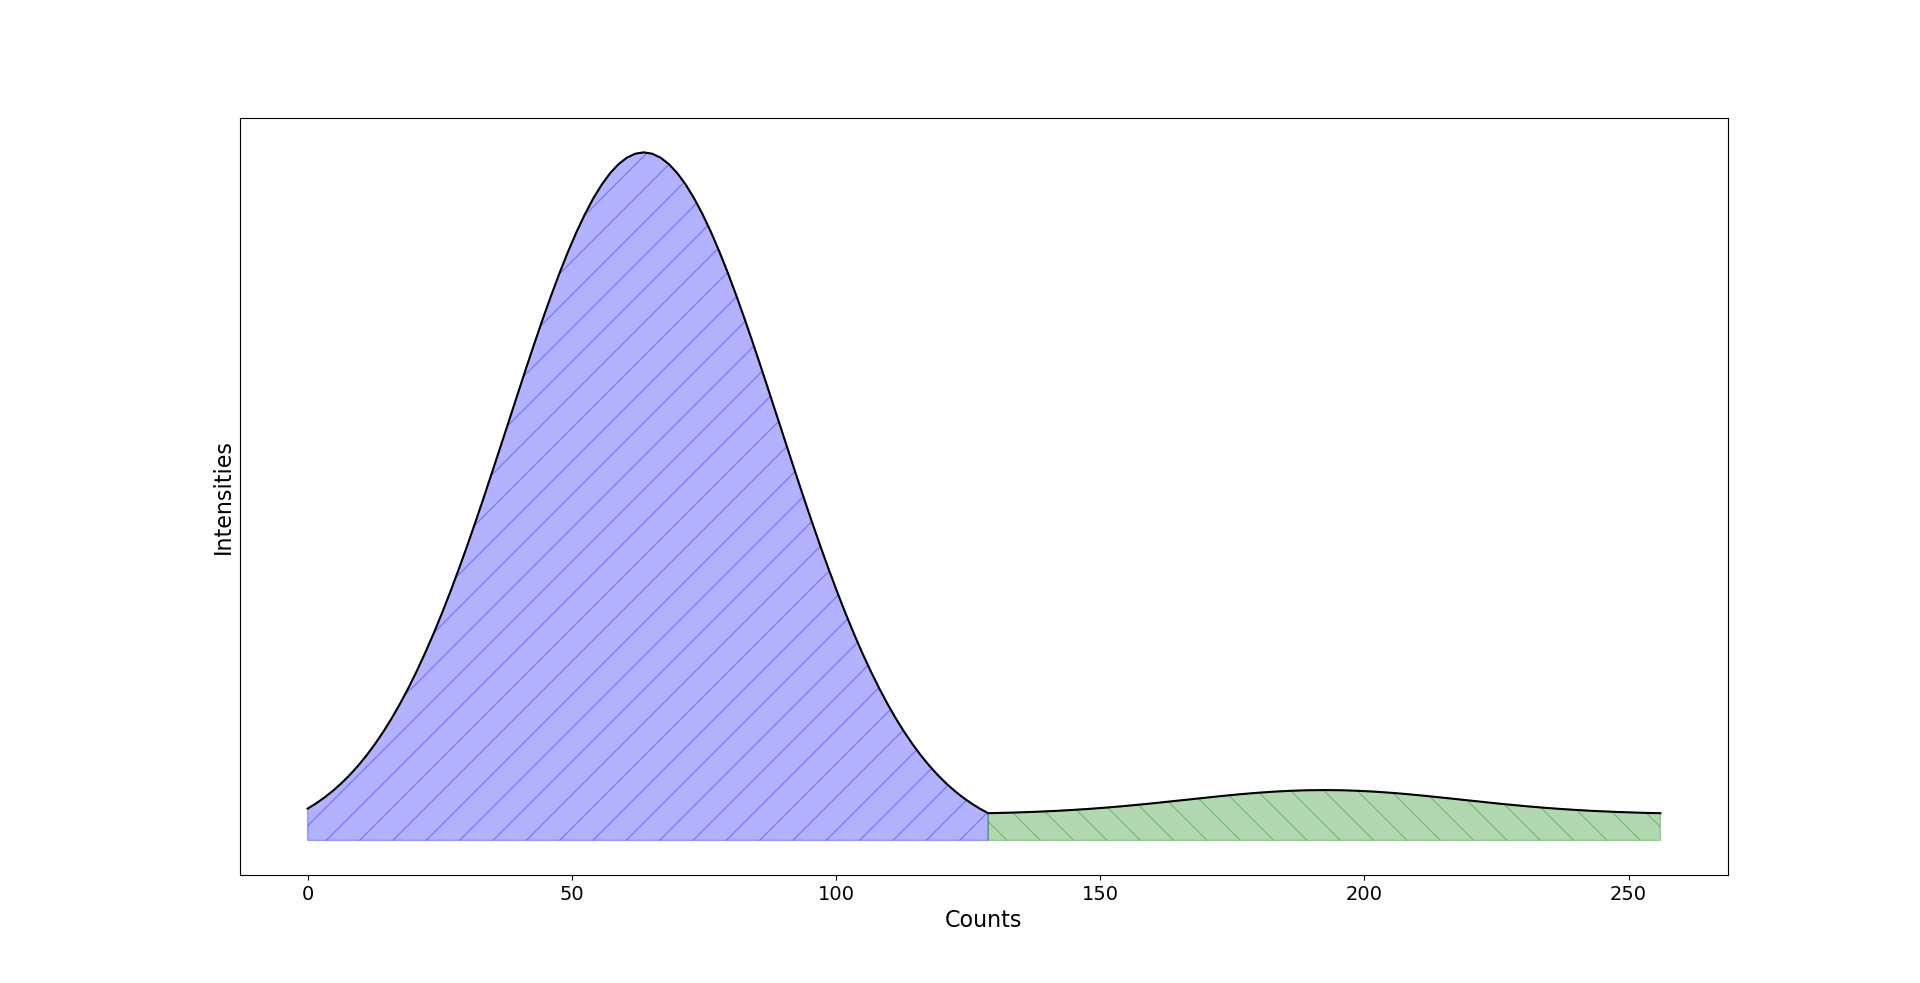
\includegraphics[width=0.32\linewidth]{figs/ch2figs/dominant_background.png}}
    \caption[Three common histogram modalities]{Three common histogram modalities with each mode being visually labelled with different colours and hatching (blue vs green and hatching direction).}
    \label{fig:histogram_appearances}
\end{figure}
When there are distinctly two peaking crests with limited overlaps of their bodies in the trough (as indicated in Figure \ref{fig:histogram_appearances}) then the histogram is referred to as bimodal. The further the histogram shape diverges from bimodal the less effective global thresholding becomes as the threshold value to separate the foreground and background becomes less clear. When this threshold value becomes uncertain then there is a greater risk of false classification of either background or foreground pixels. The greater the quantity of noise and artefacts, particularly of intensities close to the foreground pixel intensities, the worse global thresholds perform.
\paragraph{Local thresholding}
These threshold methods address this sensitivity to the histogram shape deviating from bimodal (which can be caused by noise, artefacts, and uneven illumination among others) by evaluating the image itself. This is achieved by performing calculations within sub-regions of the image and applying the threshold value derived by these calculations to this sub-region itself~\cite[p. 72]{bioimage_book}. A notable local thresholding method is \textit{Adaptive thresholding}~\cite[p.162]{segmentation_book} which calculates some threshold value by applying an operation across the pixel values within a square neighbourhood of shape $n\times n$ where $n$ specifies the size of the neighbourhood. The neighbourhood is of an odd size so that the centre of the neighbourhood can be on the currently thresholded pixel. The operation applied to the neighbourhood to calculate said threshold, in \textit{adaptive thresholding}~\cite{adaptive_thresh_plugin}, typically being that of the mean or the weighted (Gaussian) mean of the neighbourhood and potentially further tuning of the threshold strictness by the subtraction of some constant.\par Some adaptive thresholding approaches employ the variance or standard deviation of pixel neighbourhoods as a thresholding criterion but there is no definitive adaptive thresholding approach as each was developed under a specific use case. Of note is that Adaptive thresholding is sensitive to neighbourhood size as the threshold is determined by the local mean and/or variance. The threshold employed is basically that the greater the magnitude of the central neighbourhood pixel, currently being thresholded, than the surrounding pixels then the higher the likelihood it will be preserved yet if the central pixel magnitude is quite similar to, or less than, the surroundings then it is removed. This functions well for high-contrast object edges and neighbourhoods large enough to capture both background and object pixels since neighbourhoods that are too small (fit entirely within the object with minimal background) can lead to loss of object pixels if the pixels composing the object are relatively homogeneous which is more typically inside object bodies with the greatest contrast typically being between objects and the background. Likewise, overly large neighbourhoods risk approximating the shortcomings of global thresholds when applied to this data which is that across the image the distribution of intensities between background and foreground is uneven. Adaptive thresholding methods have been implemented in \textit{OpenCV}~\cite{opencv_library} and \textit{imageJ}~\cite{adaptive_thresh_plugin} by the method described above. Examples of alternative methods have been presented by \textit{A New Local Adaptive Thresholding Technique in Binarization}~\cite{Singh2012ANL} and \textit{Adaptive Document Binarization}~\cite{adapt_sauvola}. 

\section{Further investigation into prominent deconvolution and image quality restoration methods}\label{sec:further_methods}
%Here we will discuss Richardson-Lucy for deconvolution, Otsu, Hysteresis, Triangle.
\subsection{Otsu thresholding}
Otsu Thresholding is an automatic thresholding method that determines a threshold to separate two classes of intensities within an image. These classes each occupy continuous ranges of grey levels (to be referred to as intensity values) across the image histogram such that the lower class will occupy a range of $1$ to $k$ and the upper class will occupy a range of $k+1$ to $L$ where $L$ is some maximum intensity for an image and $k$ is some determined intensity threshold for the image~\cite{Otsu1979ATS}. This threshold ($k$) is selected such that the variance within each class, the variance between both classes and the variance across the image is maximized. The Otsu threshold is not without shortcomings as a prominent issue is it requires the image to be bimodal (or at least approximately bimodal) such that it can determine an optimized threshold value.\par Images with multi-modal histograms or images with noise that disrupts the desired modality of the image result in inaccurate threshold values. Over the years Otsu thresholding has been built upon in multiple papers to either improve the performance or to address multiple shortcomings. One such development resulted in an Otsu thresholding adaptation that can determine multiple thresholds for multi-modal images~\cite{MultiOtsu} but requires the expected number of classes to be provided before calculation. This is challenging in cases where the number of classes is unknown or the imaging conditions are such that the variance criteria are unrelated to legitimate classes creating confusion in the determined thresholds. In a theoretical and ideal example (illustrated in Figure \ref{fig:hypothetical_bimodal}), the threshold of a bimodal image will be within the valley between two peaks on the histogram where the between-class variance is maximal but in a case where the perceived modality is greater than one and a class expectation of two is provided, such that there are three peaks and two valleys on the image histogram, then the determined threshold may fall within either valley. In summary, Otsu thresholding performs best when the image histogram modality is two or more, the number of classes is known (the modality) and there are no aberrations across the histogram due to noise or other imaging conditions such that the modality of the image histogram is uncertain.

\begin{figure}
    \centering
    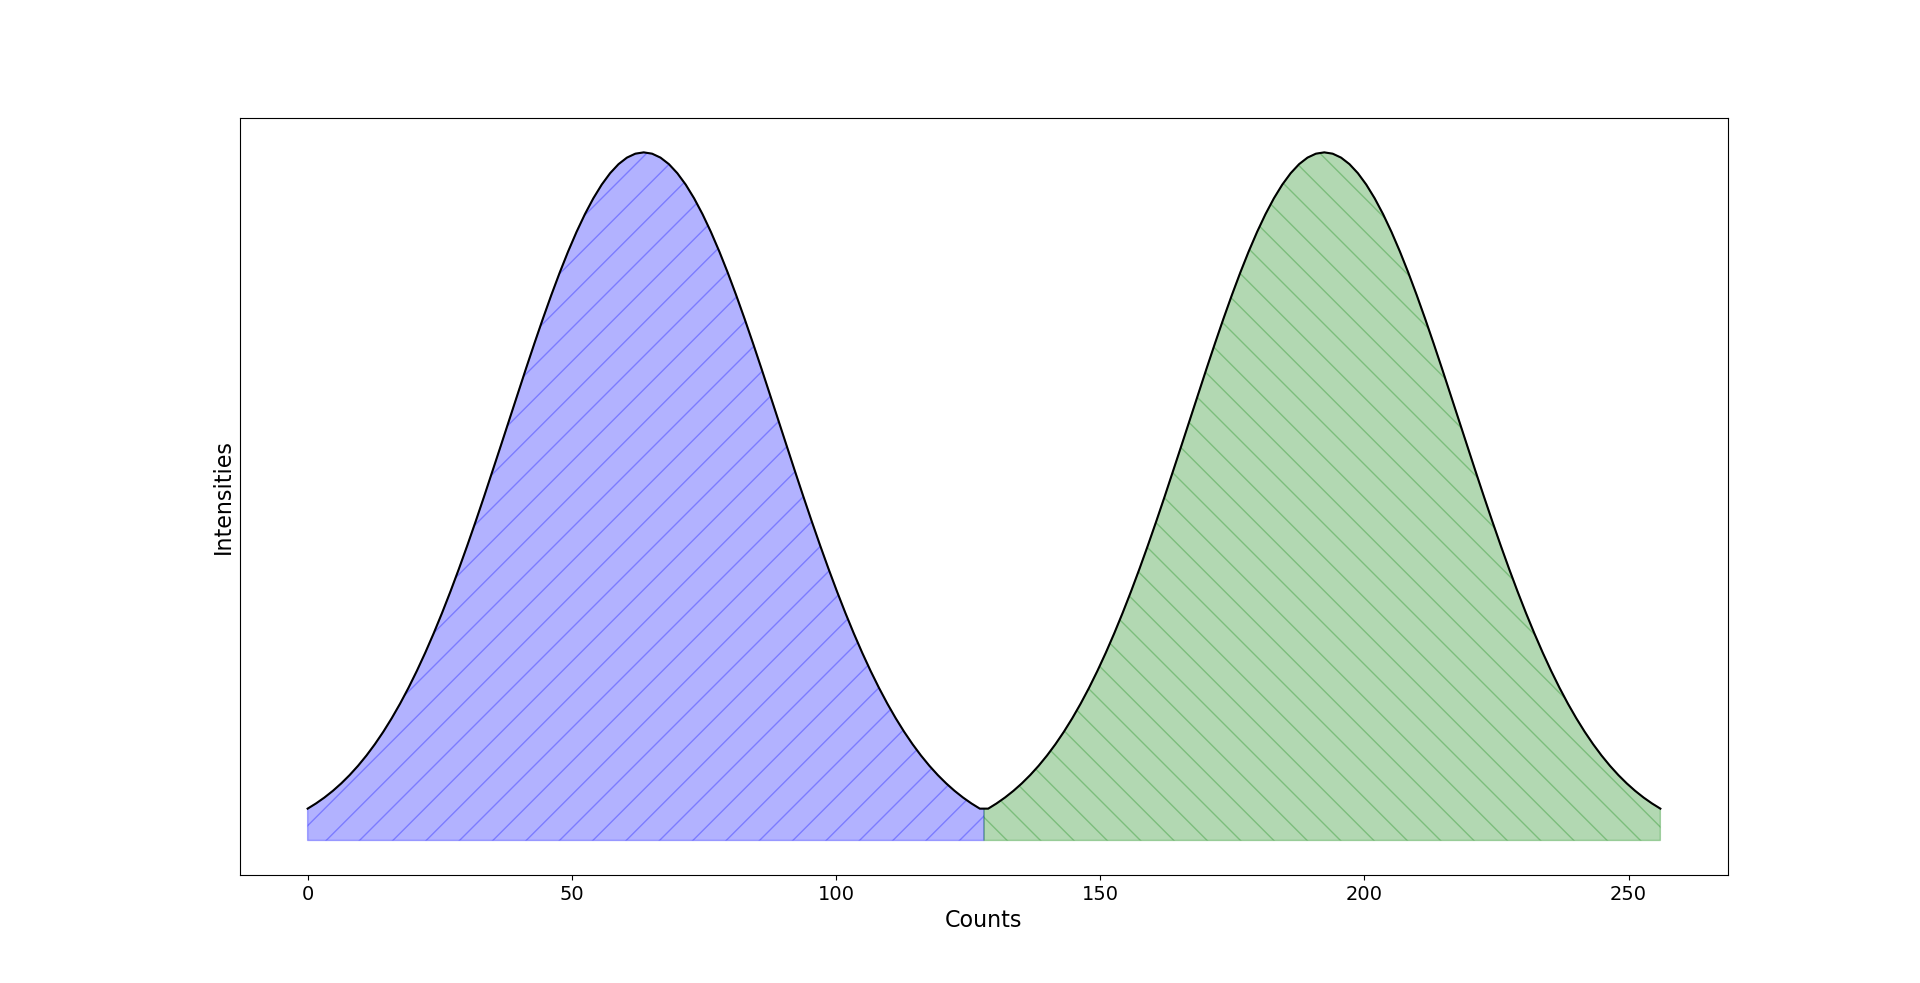
\includegraphics[width=\textwidth]{figs/ch2figs/Bimodal.png}
    \caption[A hypothetical and ideal bimodal distribution with the two modes separated in the centre]{A hypothetical and ideal bimodal distribution with the two modes separated in the centre. Each mode is defined by different colours and hatching styles with the separation point being at the ideal threshold value}
    \label{fig:hypothetical_bimodal}
\end{figure}
\par\textcolor{red}{Do you think the bimodal distribution (Fig. \ref{fig:hypothetical_bimodal}) is sufficient for the explanation of the behaviour of Otsu with an ideal modality?}

\subsection{Hysteresis thresholding} \label{sec:Hyst}
Hysteresis thresholding technique that utilizes two thresholds and evaluates pixels/voxels, for the remainder of this description pixels/voxels will be referred to as pixels, relative to their surrounding pixels for threshold application. The application of hysteresis thresholding is such that there are two provided thresholds where one can be designated as the high threshold $T_{Upper}$ and the other is to be designated $T_{Lower}$ where $T_{Upper} \geq T_{Lower}$ and $T_{Upper}, T_{Lower}\in\Re$. Across the image, any pixels greater than the $T_{Upper}$ than those pixels are immediately retained and any pixels below the $T_{Lower}$ are removed. For pixels that have a value between the $T_{Upper}$ and $T_{Lower}$, if it has a neighbouring pixel that has been retained (such as pixels with a value above $T_{Upper}$) then that pixel will also be retained. Thus structures containing pixels with continuous segments of pixels with values above the $T_{Lower}$ which connect to pixels with values above the $T_{Upper}$ are retained. It can be approximated that $T_{Upper}$ has significant control over the number of structures and that $T_{Lower}$ determines the possible volume of these structures where structures refer to continuous segments of pixels that represent some structure of interest in the image specimen/subject. A caveat of the Hysteresis threshold is the bias towards erroneously joining spatially close segments for values of $T_{Lower}$ that are too low thus indirectly affecting the structures count. One of the earliest descriptions of this method is in \textit{A Computational Approach to Edge Detection}~\cite{Hysteresis} where the method was applied to address streaking in images. where edge contours in images where streaking are \textit{``the breaking up of an edge contour caused by the operator output fluctuating above and below the threshold along the length of the contour''}~\cite[p. 689-690]{Hysteresis} which was described to be a problem more prevalent with single threshold value methods. An example of Hysteresis thresholding an the influence of erroneously selected threshold parameter values are shown in Figure \ref{fig:hyst_comparisons}.
%Add the 3D images with the sea level and mountains metaphor here so as to close off the understanding of what is considered a continuous contour
\begin{figure}
    \centering
    \subcaptionbox{The flattened maximum intensity projection (MIP) of the specimen image before Hysteresis\label{subfig:before_hyst}}{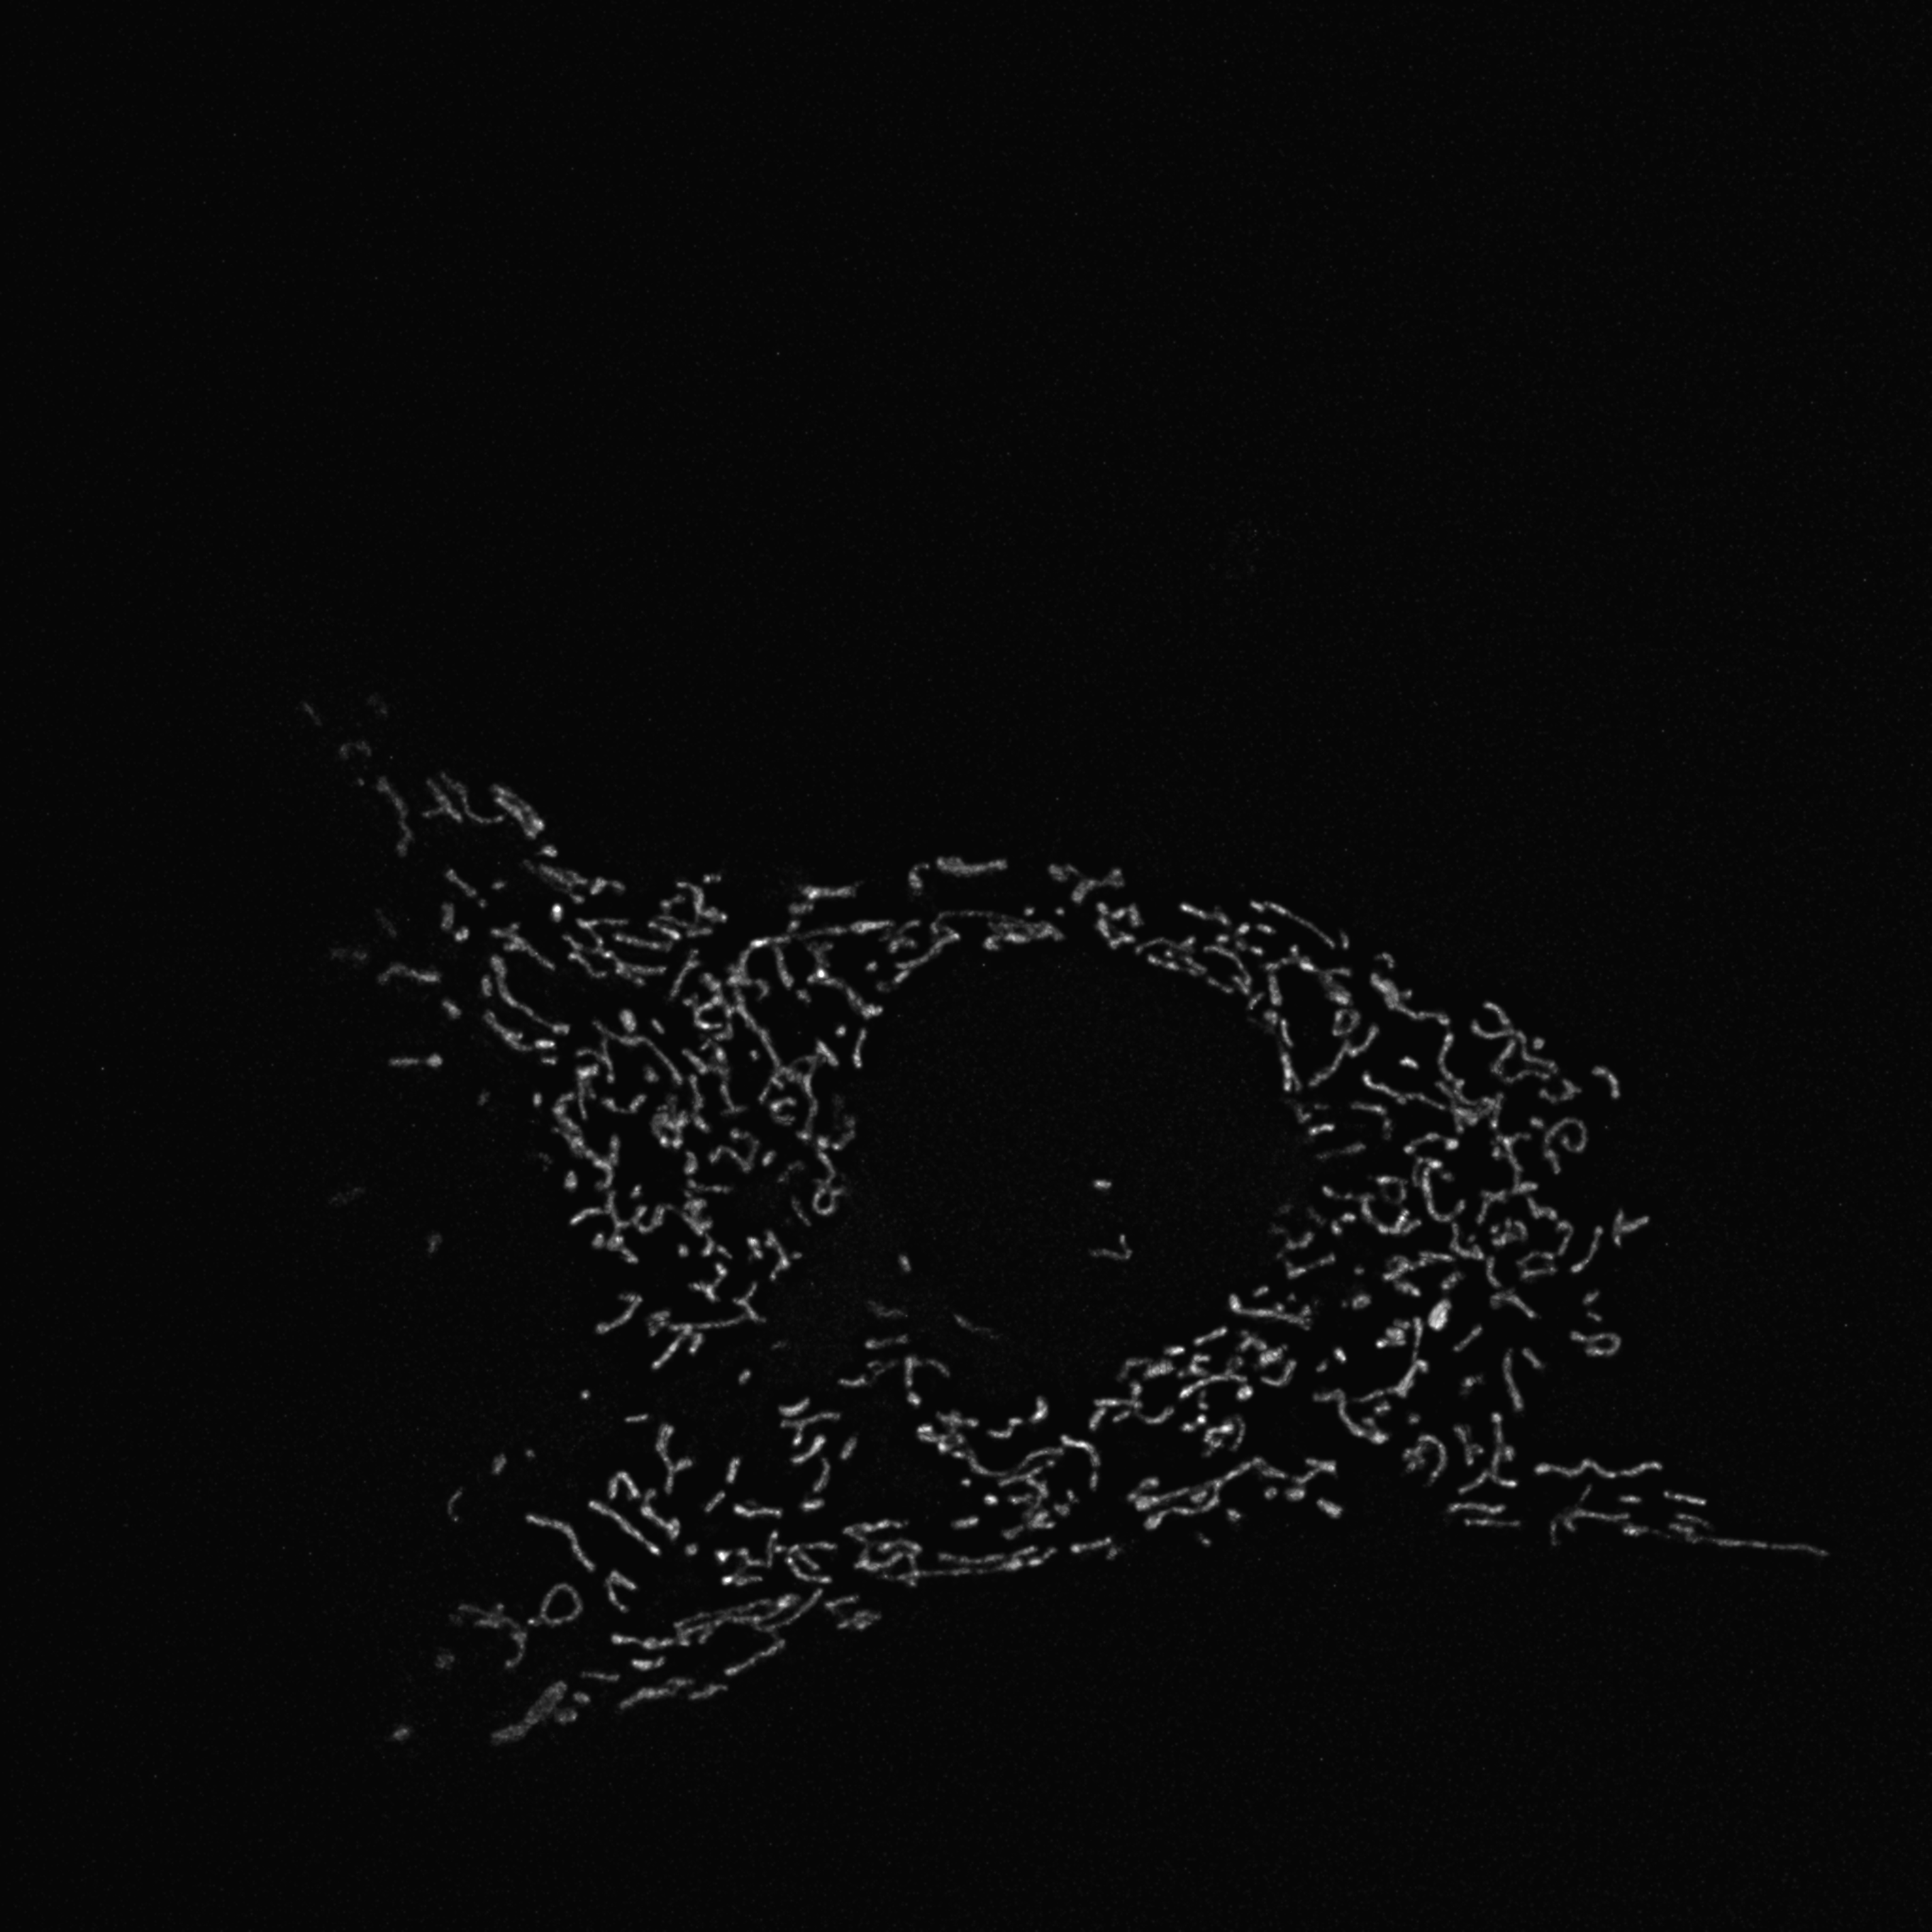
\includegraphics[width=0.49\textwidth]{figs/ch2figs/CCCP_1C=1T=0_normal.png}}
    \subcaptionbox{MIP with Hysteresis applied with good high and low threshold values\label{subfig:good_hyst}}{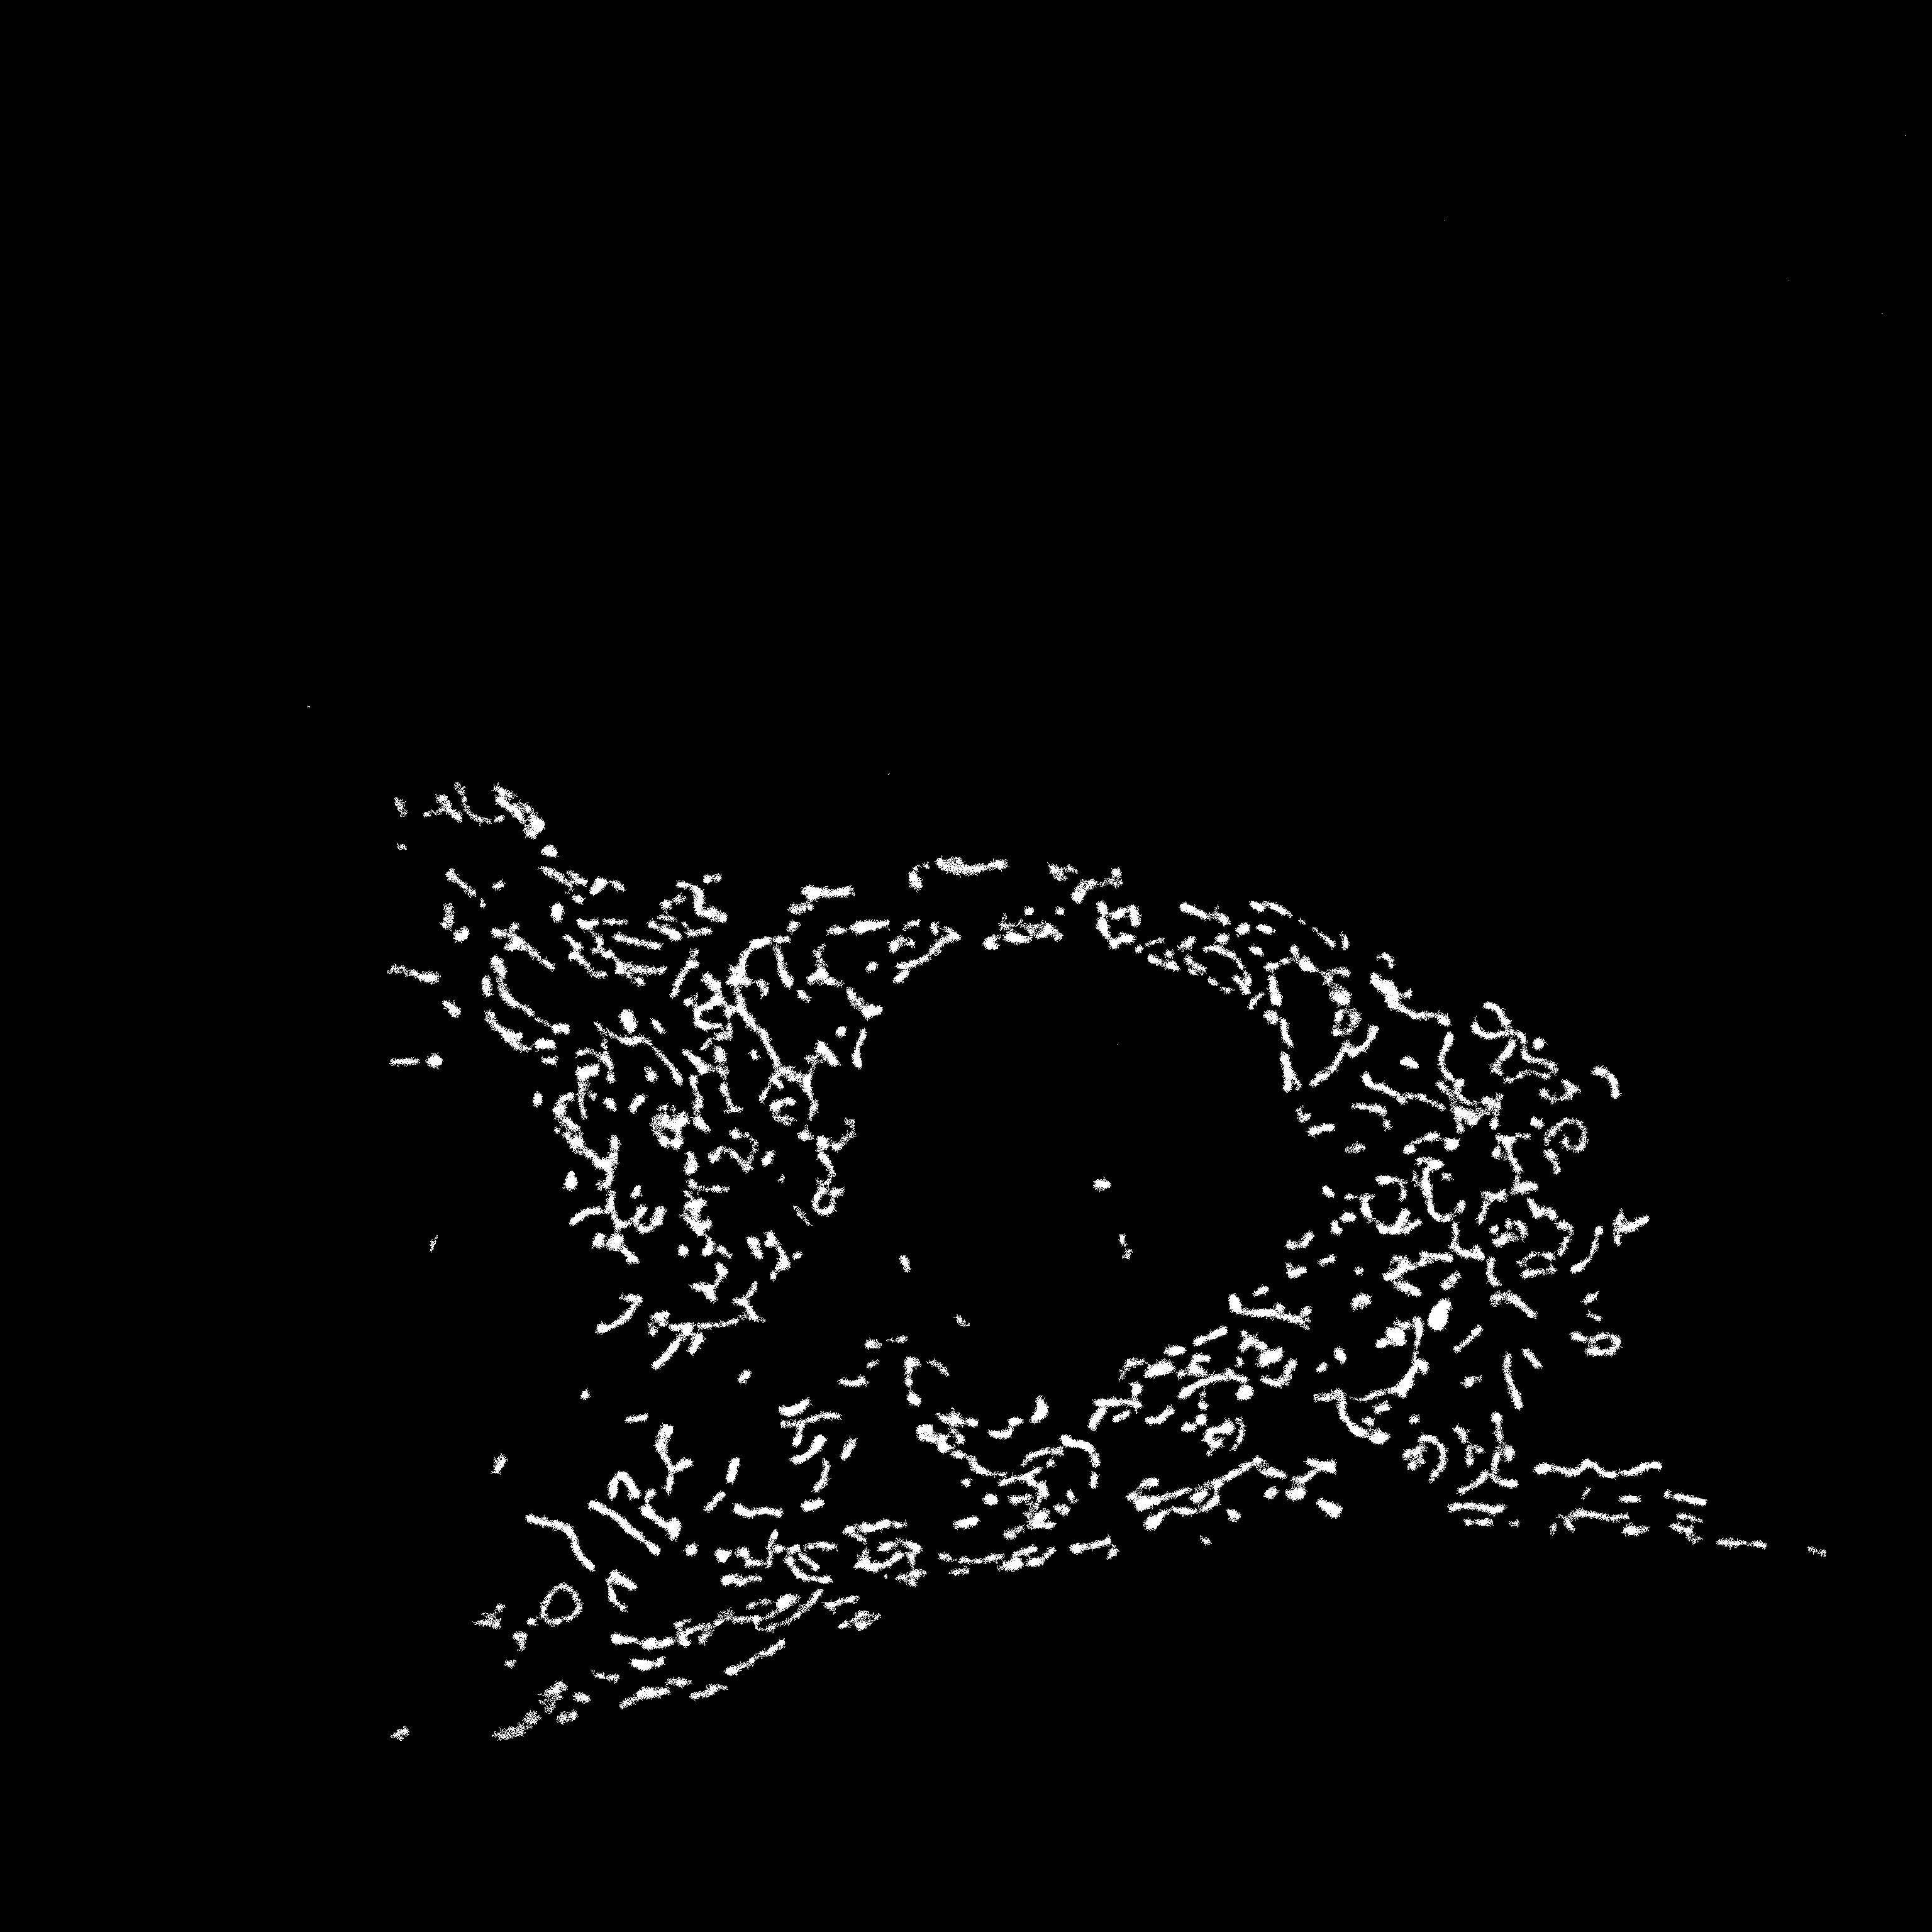
\includegraphics[width=0.49\textwidth]{figs/ch2figs/HystBin_CCCP_1C=1T=0_HystGood.png}}
    \subcaptionbox{MIP with Hysteresis applied with an overly strict (high) high threshold value retaining less individual structures\label{subfig:strict_hyst}}{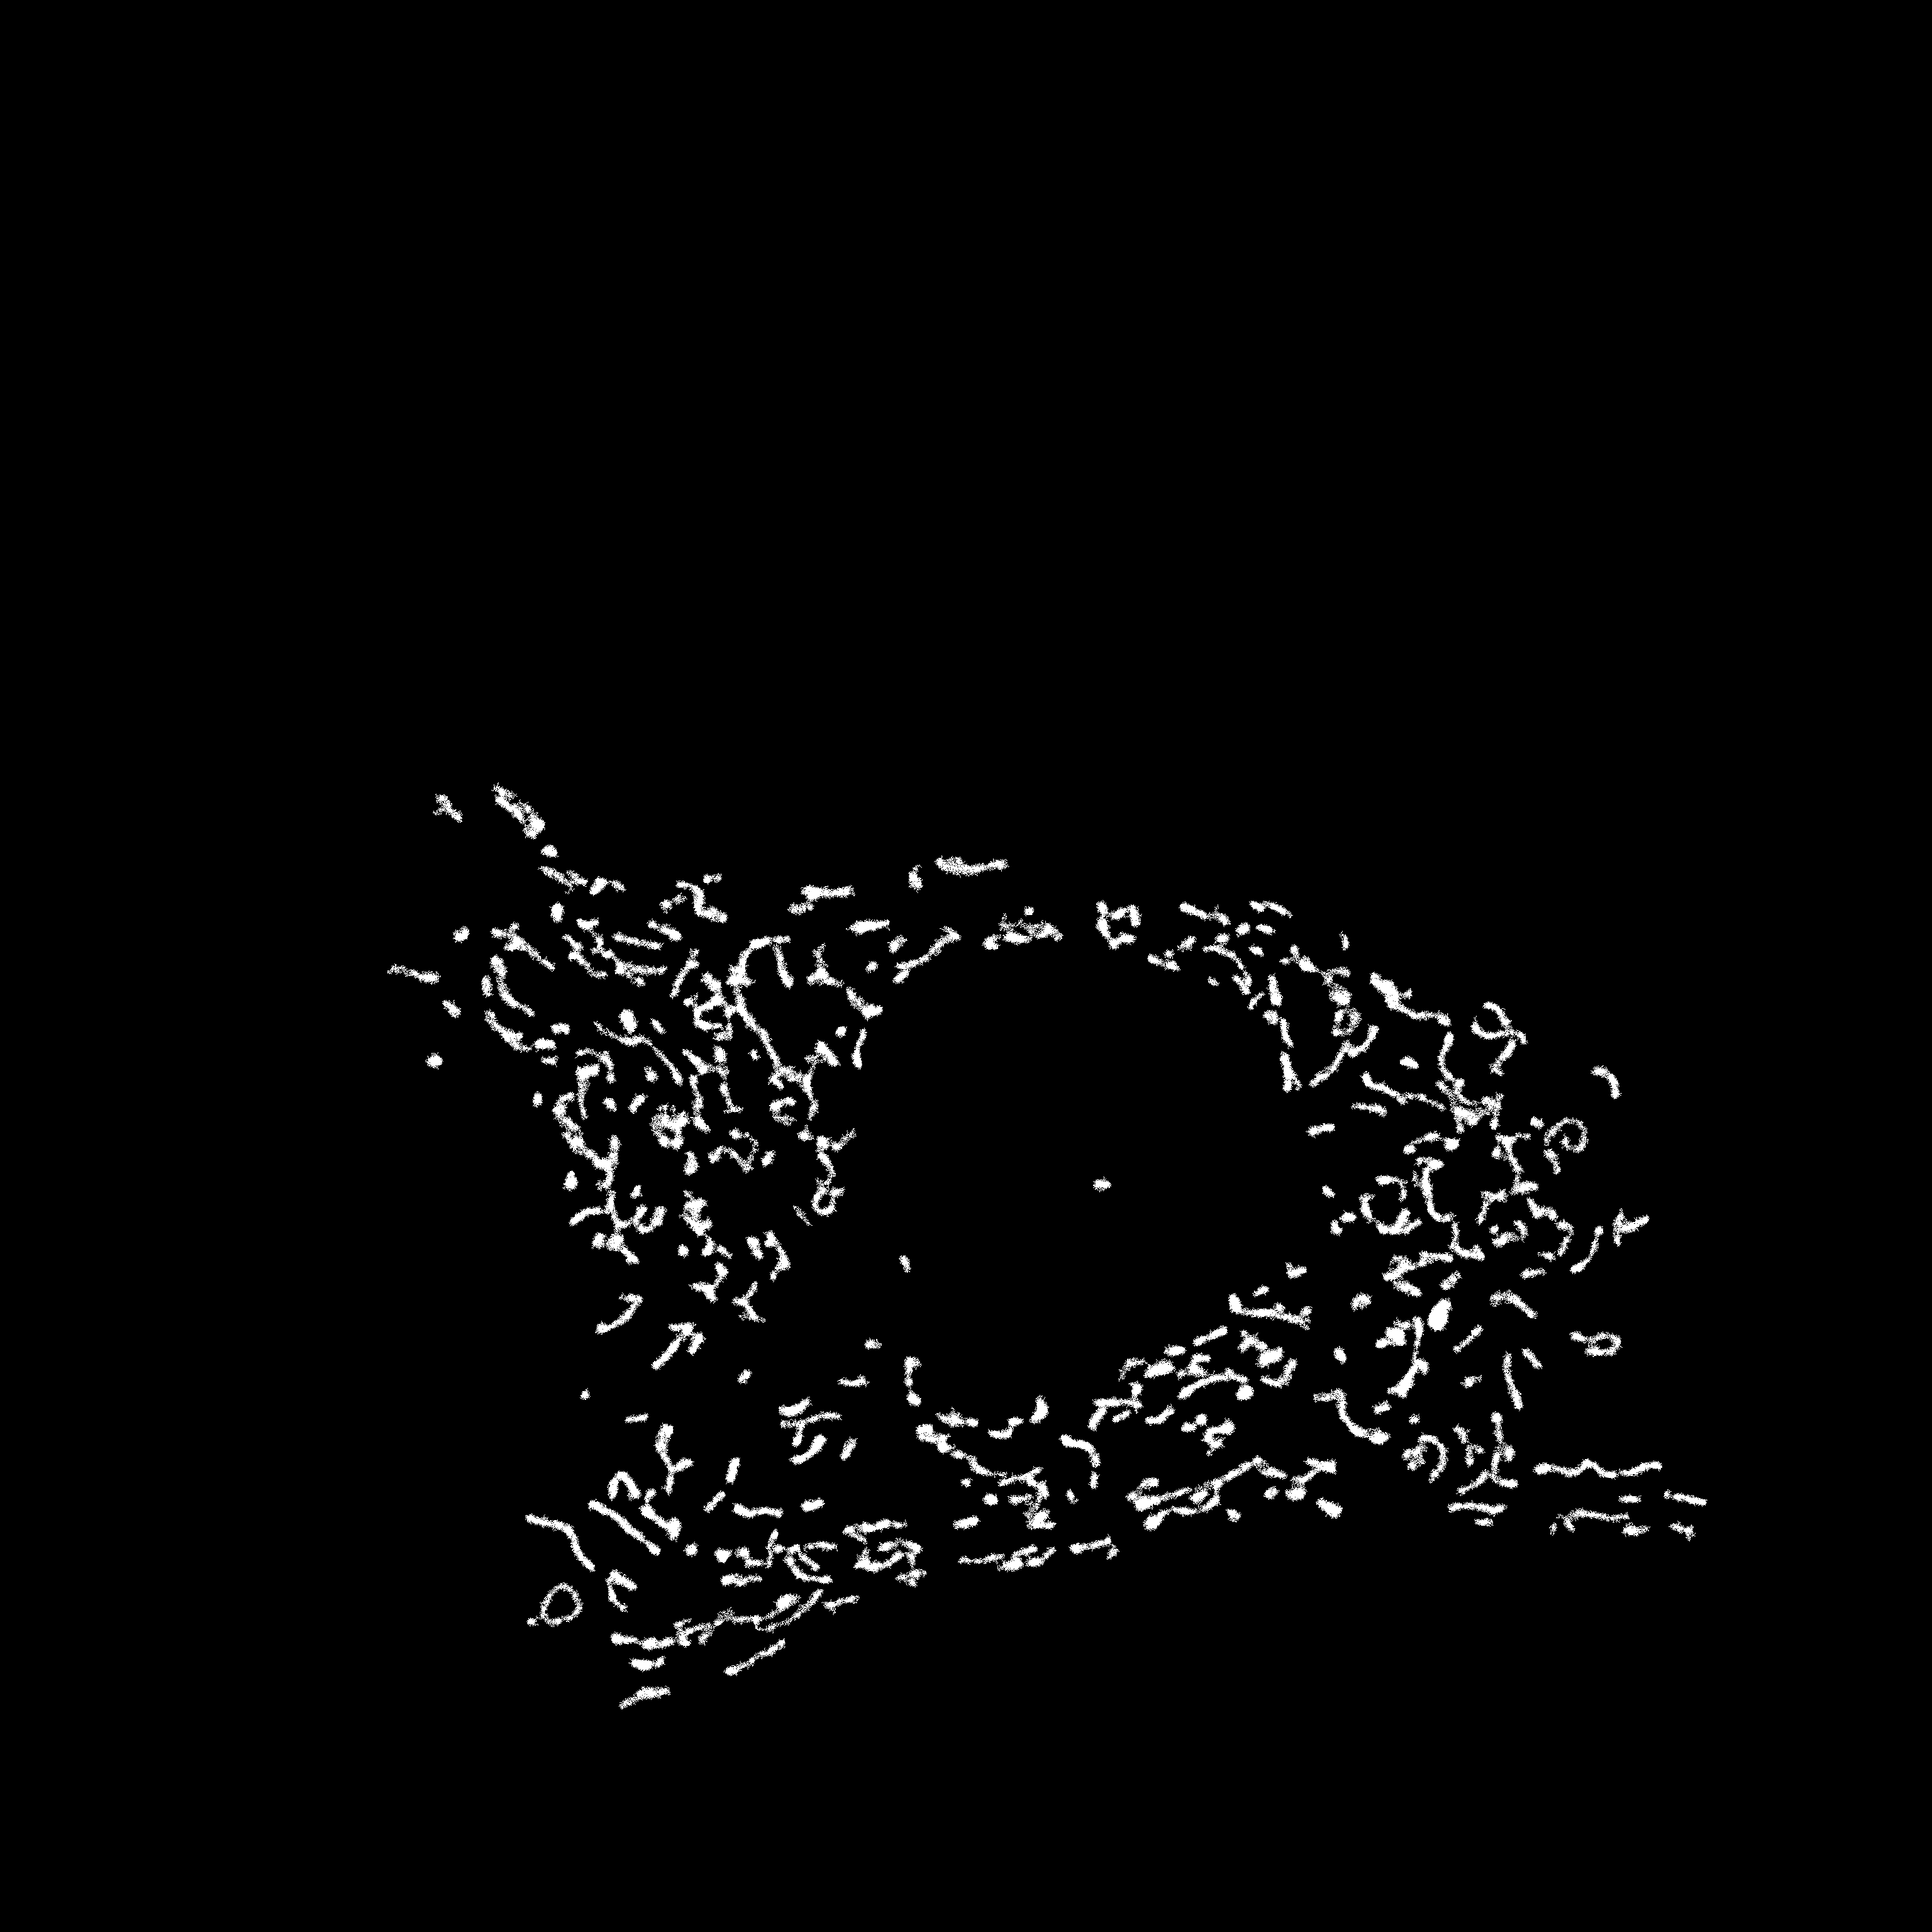
\includegraphics[width=0.49\textwidth]{figs/ch2figs/HystBin_CCCP_1C=1T=0_HighStrict.png}}
    \subcaptionbox{MIP with Hysteresis applied with an overly lax (low) low threshold retaining volume that is outside of the expected structures\label{subfig:lax_hyst}}{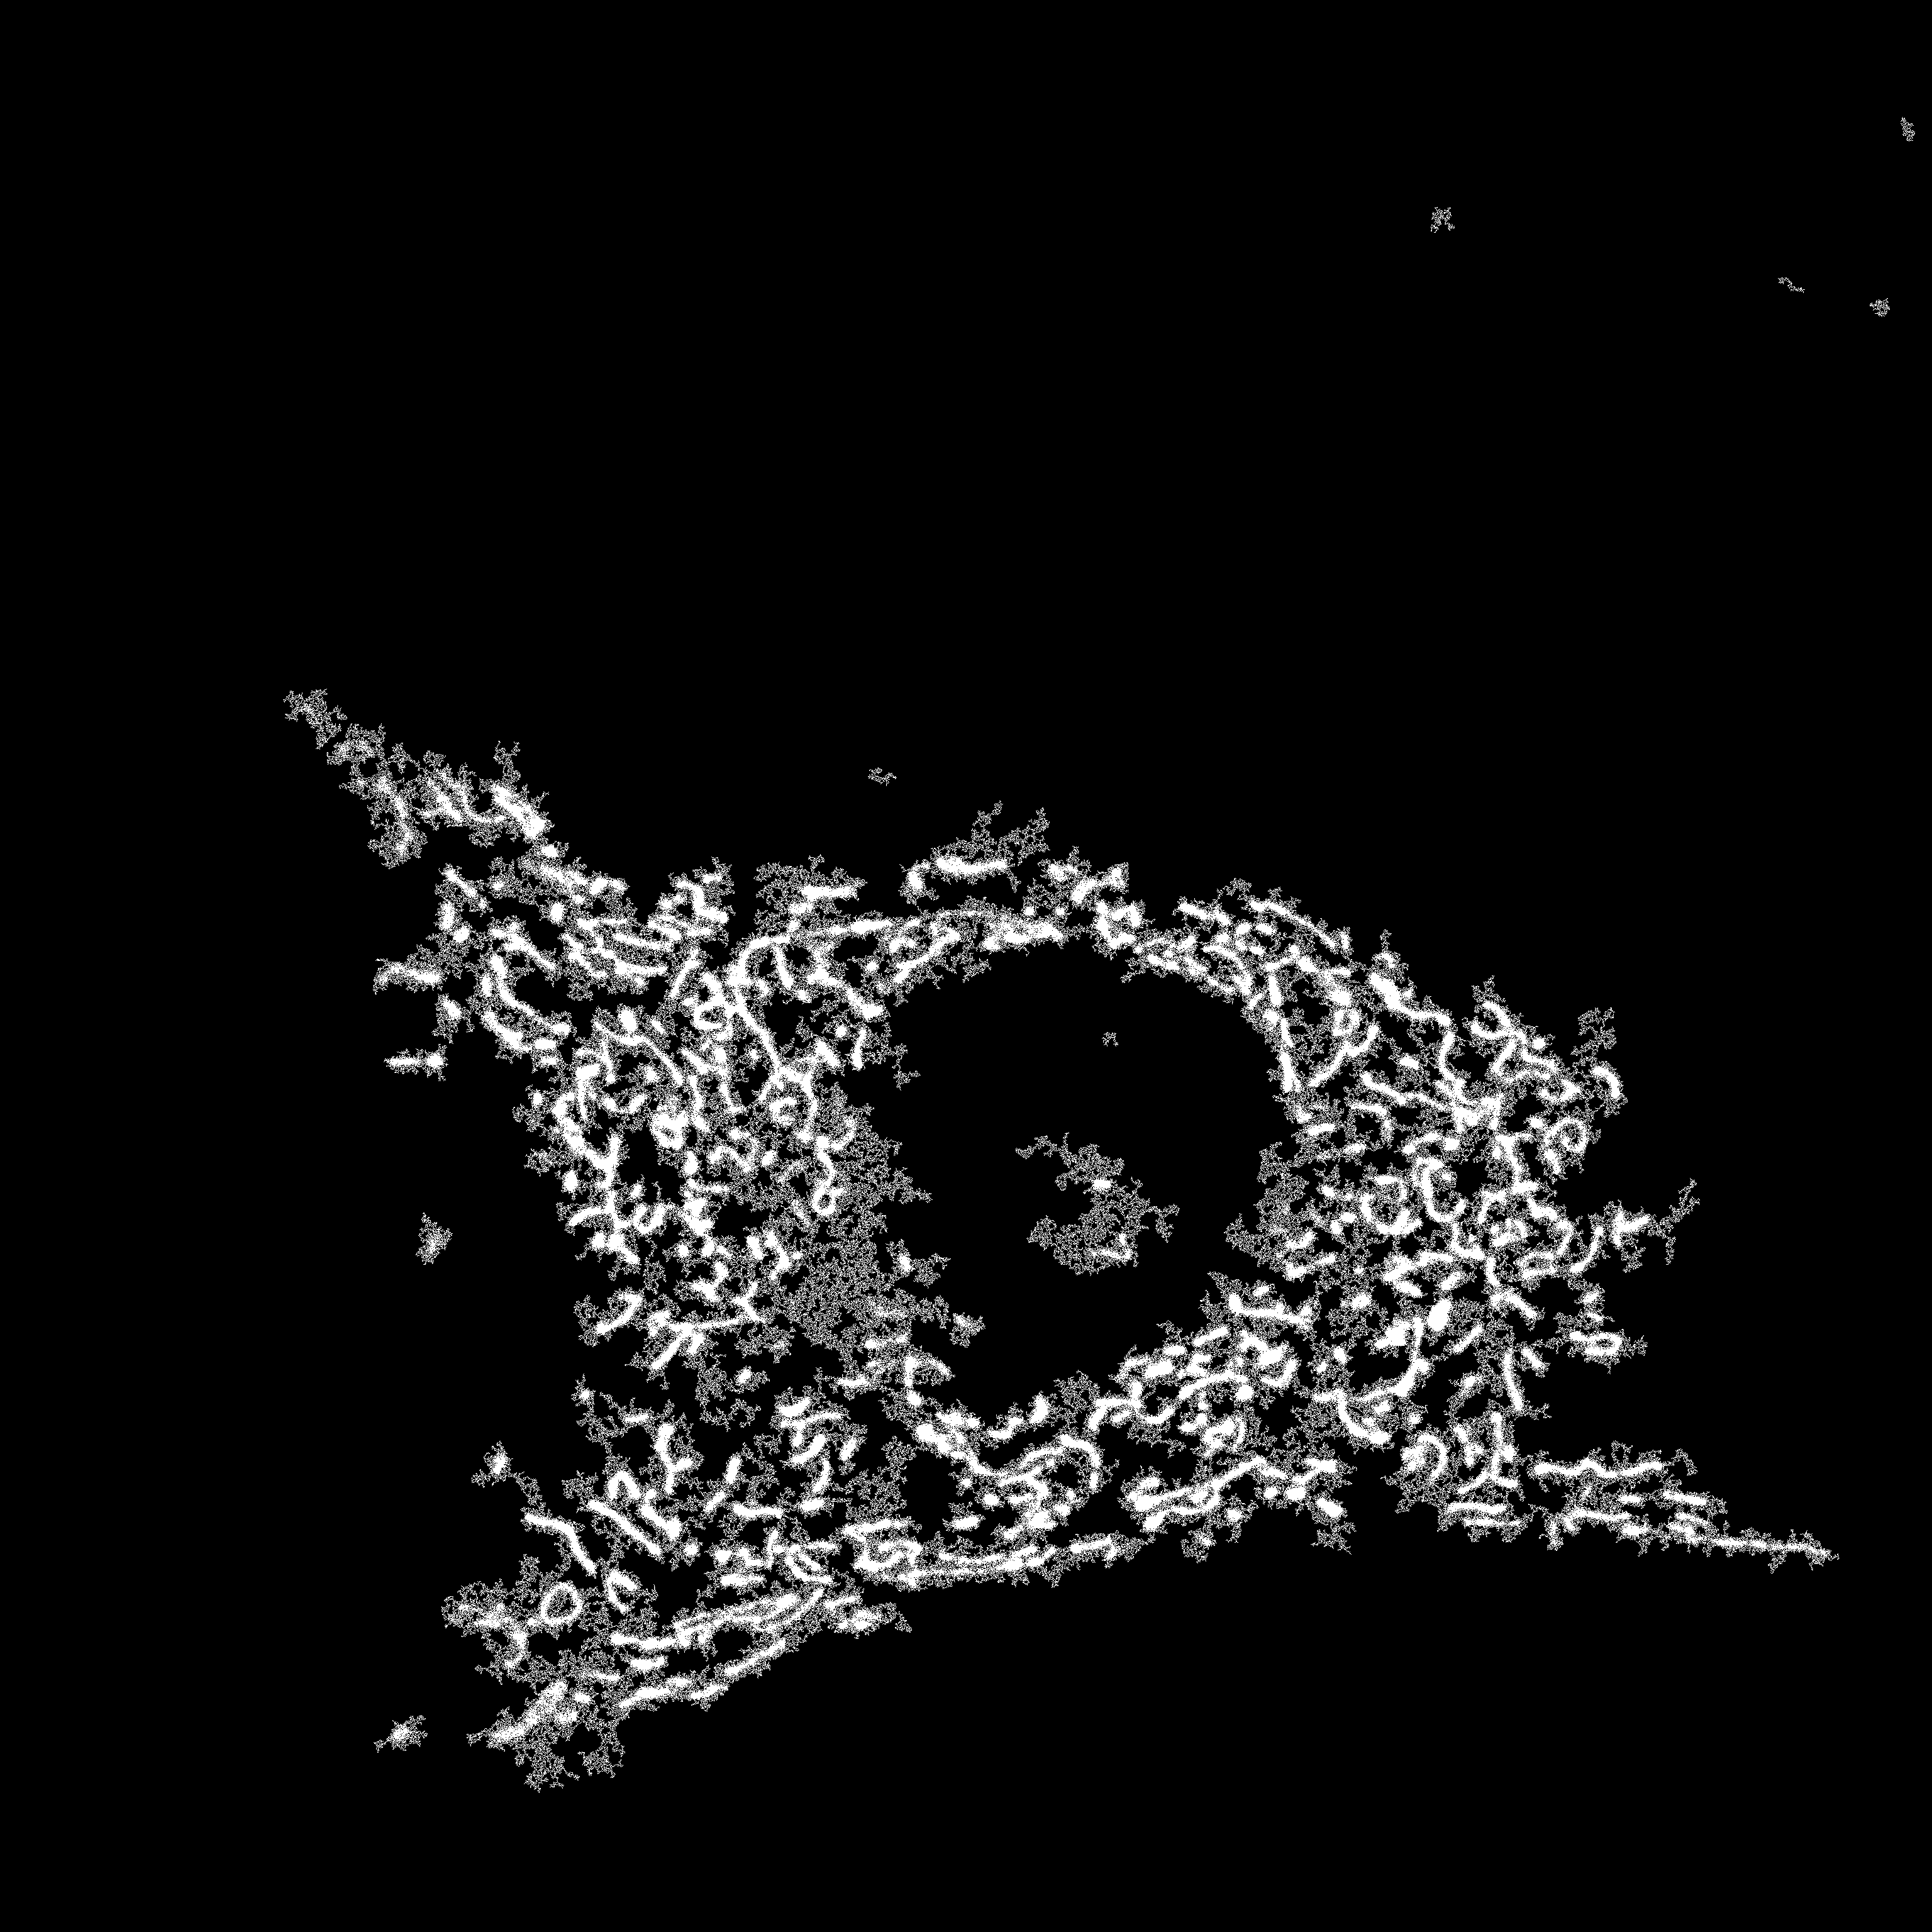
\includegraphics[width=0.49\textwidth]{figs/ch2figs/HystBin_CCCP_1C=1T=0_LowLax.png}}
    \caption[Comparison of the effect of Hysteresis threshold parameters]{Comparison of the effect of Hysteresis threshold parameters with the: \subref{subfig:before_hyst}) original image before thresholding, \subref{subfig:good_hyst}) sufficient low and high thresholds, \subref{subfig:strict_hyst}) overly strict high threshold, and \subref{subfig:lax_hyst}) overly lenient low threshold shown}
    \label{fig:hyst_comparisons}
\end{figure}
%Stuff that can be added to here as to why it is desired. Otsu finds a value to apply a high pass filter with (Hysteresis low threshold) "The key point of this threshold method is to both remove noise and isolate fluorescently stained biological structures of interest that are within focus from potential structures that are out of focus or belong to fluorescence wavelength bleeding through from another fluorescent stain type. Since this undesired fluorescence within the image needs to be separated by removing said structure without removing the fluorescence of a similar intensity in desired structures"
\subsection{Triangle thresholding}
Triangle thresholding is a method by which a triangle's geometric properties are applied to the histogram to determine the threshold. This method was employed in \textit{Automatic Measurement of Sister Chromatid Exchange}~\cite{triangleThresh} and a provided figure, shown in Figure \ref{fig:triangleThresh}, is used to visualise the logic employed. The peak intensity count value of the histogram is used as the height of the triangle and the range of intensity bins from the tail end of the histogram to the bins corresponding to the peak intensity  is used as the triangle width. The tail end will always be in the direction of the histogram that is further from the peak value bin. The tail end is the longer length of the histogram bin range originating from the bin of the peak intensity count and either the upper or lower bounds. The lower bound is generally the zero bin and the upper bound is usually the bin corresponding to the maximum intensity value of the image. This can be seen in the third line of equation \ref{eq:tail_flip} where $N$ is the maximum number of histogram bins; $h(n)$ is the bin count for the corresponding bin $n$; $n_{peak}$ is the bin with the maximum number of bin counts; $h_{peak}$ is the maximum number of counts for a bin in the histogram; and $W$ is the width from the peak bin $n_{peak}$ to the further bound which is either the lower or upper bin range bound. 
\begin{equation}\label{eq:tail_flip}
\begin{split}
    h(n) &= hist(image) \text{ where } n \in N \\
    h(n_{peak}) &= h_{peak} = max(\mathbf{h})\\
    W &= max(N - n_{peak}, n_{peak}) \\
\end{split}
\end{equation}
With the triangle height and width established the hypotenuse of the triangle can be determined. Using the hypotenuse, a perpendicular line is measured from the hypotenuse to the histogram count value at a corresponding bin $n$ where the bin $n$ which provides the maximum perpendicular length is used as the threshold intensity.
\begin{figure}[h]
    \centering
    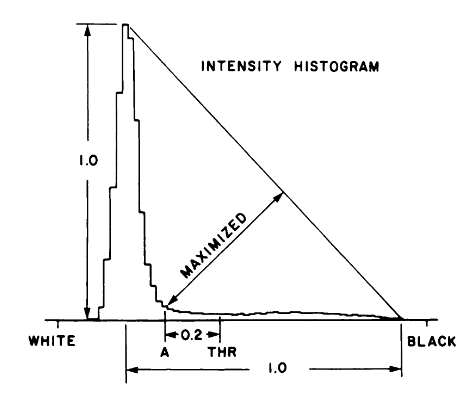
\includegraphics[scale=0.5]{figs/TriangleThresholdRef.PNG}
    \caption[Depiction of normalized histogram with annotated measurements for threshold selection]{Depiction of normalized histogram with annotated measurements for threshold selection\cite[p.742]{triangleThresh}}
    \label{fig:triangleThresh}
\end{figure}
\par This method functions well when the threshold being sought is situated close to the peak within the histogram. When this peak represents noise then the method is more effective when the angle from the peak value to the desired threshold value is steeper. If there are multiple modes in the histogram due to different noise sources or imaging properties then it can be more challenging to select an effective threshold value. This is due to the likelihood of the maximal perpendicular lengths being jointly dependent on the observed bin's closeness to the peak bin and the bin count value where the likelihood increases as the observed bin tends to the peak bin and the bin count value is lower. Figure \ref{fig:triangles} shows a series of hypothetical triangles to illustrate the impact of histogram shape on the threshold value calculations. In Fig. \ref{subfig:triangleA} the perpendicular lengths range from $L1$ to $L3$ with the chosen thresholds following the same order (to say that if $L1$ was ignored then $L2$ would be the next best threshold) where these distances are a limited subset for illustration, all bin count values will have a corresponding length. In Fig. \ref{subfig:triangleB} and \ref{subfig:triangleC} the effect of the histogram shape can be seen where the former depicts either a bimodal or dominant background bimodal histogram while the latter depicts a multimodal histogram. The bimodal histogram still presents the lowest illustrated bin value corresponding to $L1$ as the best threshold since the separation between the two modes allows a large length to that bin. The multimodal histogram shows that the multiple modes, or crests, increase the difficulty in selecting the correct threshold as there is no clear separation and both $L1$ and $L2$ are similar in value (Fig. \ref{subfig:triangleC}). Image contrast can stretch the histogram providing greater resolution to separate these modes and false modes induced by noise in the image (making it appear multimodal) can impair the effectiveness of this threshold. Based on this Triangle thresholding is effective when there are bimodal or dominant background histograms but is sensitive to noise and inappropriate adjustments to the histogram shape. \textcolor{red}{The main references are towards the beginning of this subsection which also informs later explanations but I did not explicitly reference them as part of this is from my inference of the method. Do you think I should cite those same sources again at this later point for credibility?}

\begin{figure}
\centering
\begin{subfigure}[t]{0.3\textwidth}
    \centering
    \resizebox{!}{4.4cm}{
    \input{figs/TriangleFigA.tikz}
    }
    \caption{Depiction of the perpendicular lengths from the triangle hypotenuse to the $x$-axis}
    \label{subfig:triangleA}
\end{subfigure}
\hfill
\begin{subfigure}[t]{0.3\textwidth}
    \centering
    \resizebox{!}{4.4cm}{
    \input{figs/TriangleFigB.tikz}
    }
    \caption{A slope shape that is steep but shows the impact of a crest at higher bin values due to $L2$ and $L3$ being similar.}
    \label{subfig:triangleB}
\end{subfigure}
\hfill
\begin{subfigure}[t]{0.3\textwidth}
    \centering
    \resizebox{!}{4.4cm}{
    \input{figs/TriangleFigC.tikz}
    }
    \caption{A different slope shape with a secondary, smaller peak branching off of the decline from the first peak.}
    \label{subfig:triangleC}
\end{subfigure}
\caption[A depiction of the typical trend in perpendicular distances $L$ relative to the slope shape]{A depiction of the typical trend in perpendicular distances $L$ relative to the slope shape. \subref{subfig:triangleA}) The histogram with no slope visible showing the lower $x$-axis (bin) values result in larger perpendicular distances. The impact of the slope shape is evident in (\subref{subfig:triangleB}) and (\subref{subfig:triangleC}) where the steepness in (\subref{subfig:triangleB}) results in $L1$ being the largest distance while $L2$ and $L3$ are similar despite $L2$ having a lower bin value. \subref{subfig:triangleC}) Shows the impact of a secondary peak branching off of the slope can lead to two similar lengths at different bin values. The bin ($x$-axis) value resulting in the largest perpendicular distance is used as the threshold}
\label{fig:triangles}
\end{figure}

\subsection{Richardson-Lucy deconvolution}\label{subsec:richardson_lucy}
The Richardson-Lucy (RL) deconvolution algorithm is based on the combination of two independently developed algorithms by W. Richardson~\cite{Richardson} and L. Lucy~\cite{LucyL}. For this exploration, the logic behind the algorithm will be described from W. Richardson's paper~\cite{Richardson} as it was more general focusing on image restoration as opposed to L. Lucy's~\cite{LucyL} application in the astronomical sciences field. RL deconvolution is an iterative algorithm that utilizes successive iterations to approximate a solution to minimize image diffraction. The development of this algorithm relied on a set of assumptions such as the distorted image can be represented as $H=W*S$ where $H$ is the distorted image, $W$ is the original image before distortion and $S$ is the PSF representing the diffraction which distorts the image. The second assumption is that $W$, $S$ and $H$ are probability-frequency functions such that if $i$ were some observed outcome of an event and there are $I$ total possible outcomes where $i \in I$ then there will be multiple observations $N$ where each outcome will be observed $n$ times where $n \in N$. As this is a probability-frequency function the probability of each event outcome comes to be measured from the frequency of said outcome relative to the total number of observed outcomes e.g. $P(W=W_i) = \frac{W_i}{\sum^I W_i} = \frac{n_i}{N}$. From this $W = \sum_I W_i$ where each of these function probabilities can be reduced to the observance count per outcome divided by the total number of observations across all possible outcomes. Using a single dimension $i$ is merely for descriptive simplicity and this can be expanded to multiple dimensions such that $W = \sum_{i,j} W_{i,j}$ and both $i$ and $j$ can be employed as the axis of an array or the coordinates of the pixels in an image where the outcome would be the intensity value of the pixel.\par The crux of the method relies on two equations. The first equation is the application of Baye's theorem regarding the conditional probability of an event $W_i$ given an event $H_k$ where $k$ is some observed outcome independent of $i$. The resulting formula (Eq. \ref{eq:RichBayes})~\cite[Eq. 1]{Richardson}:
\begin{equation}\label{eq:RichBayes}
    P(W_i|H_k)=\frac{P(H_k|W_i)P(W_i)}{\sum_j P(H_k|W_j)P(W_j)};\text{ }i=\{1,I\}\text{ }j=\{1,J\},\text{ }k=\{1, K\}
\end{equation}
where $H_k$ is described to be some arbitrary cell $k$ of $H$. This relationship is important as the probability of determining the correct value of $W_i$ depends on the value of $H_k$ as $H$ is the distorted image from $W$ must be restored while $W$ is not known. Since $S$ is the function of the distortion applied to each event $i$ of $W$ resulting in $H$ for some $k$ value(s) thus $P(H_k|W_i)=P(S_{i,k})=\frac{S_{i,k}}{S}$. A second consideration is that since $W_i$ is not known then the best solution is to use an estimated $W_i$ where a better estimate will result in a more accurate $W_i$. To approach this accurate $W_i$ the process is performed iteratively where each $W_i$ determined in a prior iteration is used as an estimate for the current $W_i$ estimation where $r$ is used to refer to the current iteration~\cite[Eq. 4]{Richardson}. Using both of these considerations an equation(Eq. \ref{eq:iterativeBaye})~\cite[Eq. 5]{Richardson} is determined:
\begin{equation}\label{eq:iterativeBaye}
    W_{i,r+1} = W_{i,r}\sum_k \frac{S_{i,k}H_k}{\sum_j S_{j,k}W_{j,r}}
\end{equation}
One final consideration is made due to the finite size of arrays in computers and equation \ref{eq:iterativeBaye} is changed in terms of the event summation bounds. The rewritten equation\cite[Eq. 6]{Richardson} is:
\begin{equation}\label{eq:RichardsonFinite}
    W_{i,r+1} = W_{i,r}\sum_{k=i}^c \frac{S_{k-i+1}H_k}{\sum_{j=a}^b S_{k-j+1}W_{j,r}}
\end{equation}
Where in equation \ref{eq:RichardsonFinite}, $a=(1, k-J+1)_{max}$, $b=(k,I)_{min}$, and $c=i+J-1$.For equation \ref{eq:RichardsonFinite}, W. Richardson describes that the summation over $k$ and the summation with the bounds $a$ and $b$ in the denominator appear to be a corrective measure to adjust the estimated $W_i$ over successive iterations where the denominator can compensate for escalating in value and encouraging the estimated $W_i$ to converge to some value. This compensation in one estimated element $W_{i,r}$ may be further from the final converged $W_{i,R}$ value at some iteration to improve the convergence of some other element $W_{m,r}$ where $m\in I$. The event element $i$ is one dimensional but the element variables can be expanded to account for multiple dimension arrays. A shortcoming of this algorithm is the potential for noise amplification of successive iterations although an algorithm developed from Richardson-Lucy is \textit{Richardson-Lucy with total-variation regularization} which implements a regularization term to compensate for the noise amplification~\cite[p.33]{DeconLab2}. 
\textcolor{red}{In this subsection I initially prefaced that the explanation will be based on W. Richardson's paper and I cite the individual equations I mention from his paper. Despite this do you think I need to cite him more frequently across this section?}

\section{Other techniques implemented within this research}

\subsection{Kneedle algorithm} \label{sec:kneedle}
\textit{Kneedle} is an approach to determine `knees' in a distribution~\cite{kneedle_paper}. Traditionally the knee, or elbow, of a distribution is described as some approximate point by which there is a change in the trend of the distribution. This is similar to the concept of the inflection point of the distribution but there is no standardised definition of a `knee' rather it is the visual estimation of the point performed heuristically by a human viewing the visualisation of the data. Due to this, it can be loosely defined as the point most significant to the change in the trend of the data. A visualised distribution with an estimated region in which a `knee' would be selected is shown in Figure \ref{fig:knees}.\par
\begin{figure}
    \centering
    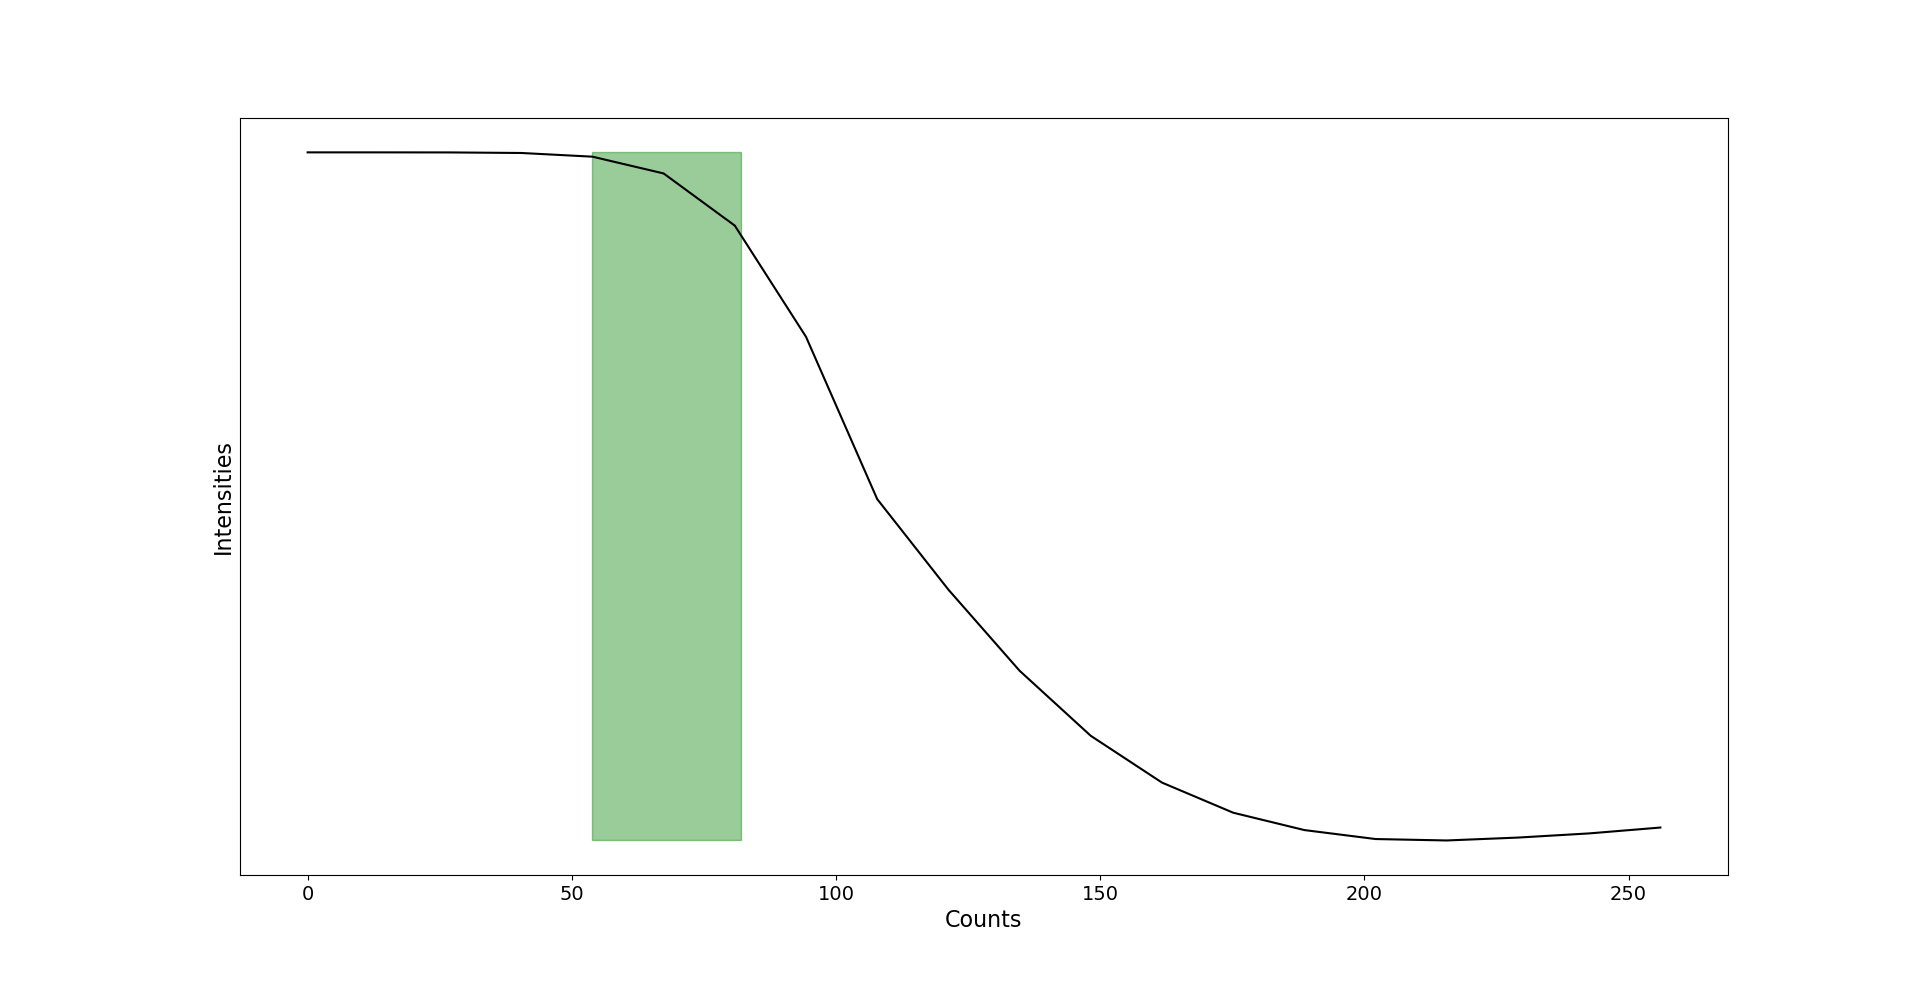
\includegraphics[width=0.7\textwidth]{figs/ch2figs/knees.png}
    \caption[Approximate knees in a graph by heuristic evaluation]{Approximate knees in a graph by heuristic evaluation. The highlighted region designates the likely region within which a knee point would be chosen. A range is displayed as the exact point is dependent on heuristic bias.}
    \label{fig:knees}
\end{figure}
One method of interest that attempts to address this is \textit{Finding a ``Kneedle'' in a Haystack:Detecting Knee Points in System Behavior}~\cite{kneedle_paper} which both presents a mathematical definition of a `knee' and the method by which this `knee' is determined. \paragraph{Knee Definition} Firstly, it was stated prior that the knee of a distribution is visually similar to that of the inflection point yet this point does not capture the point at which trends change but rather a change in the sign of the curvature of the distribution. The chosen definition is based on the curvature of a continuous definition where the point at which maximum curvature is expressed is the closest to what would be the knee point~\cite[p.2]{kneedle_paper}. The equation describing curvature ($K_f(x)$) is shown in Equation \ref{eq:curvature} where $f(x)$ is the distribution for which the curvature is being described.\par
\begin{equation}\label{eq:curvature}
    K_f(x) = \frac{f''(x)}{(1 + f'(x)^2)^{1.5}}
\end{equation}
This curvature equation performs well with continuous functions yet is challenged by discrete distributions. The causes behind these challenges are related to the incompatibility encountered when fitting a continuous function to a finite distribution as a minimum of 3 data points are required to calculate the curvature (centred on the second data point) thus the curvature for the first and final point in the discrete set cannot be determined. Another major challenge is that determination of the maximum curvature within the distribution requires this calculation to be performed across the whole discrete set and it is possible for the point of maximum curvature to exist outside the range of the finite set.\paragraph{Knee method} It is explicitly stated that \textit{``Kneedle''}, the method by which the knees are determined, is predicated on the assumption that the knee is the point expressing the maximum curvature but there can be multiple knee points within a distribution or set. For multiple points to be approximated it is the local maxima of the curvature across the set that describes a knee point. These local maxima of the curvature are determined by \textit{``that are local maxima if the curve is rotated $\theta$ degrees clockwise about ($x_{min},y_{min}$) through the line formed by the points ($x_{min},y_{min}$) and ($x_{max},y_{max}$)''}~\cite[p.3]{kneedle_paper}. Thus far the designed method presumes that the knee point is for an increasing curve that is of negative concavity but this can be performed for curves with a positive concavity (an ``elbow'' as opposed to a knee) by inverting the distribution with examples for each shown in Figure \ref{fig:knee_elbow_example}.
\begin{figure}
    \centering
    \subcaptionbox{Knee example}{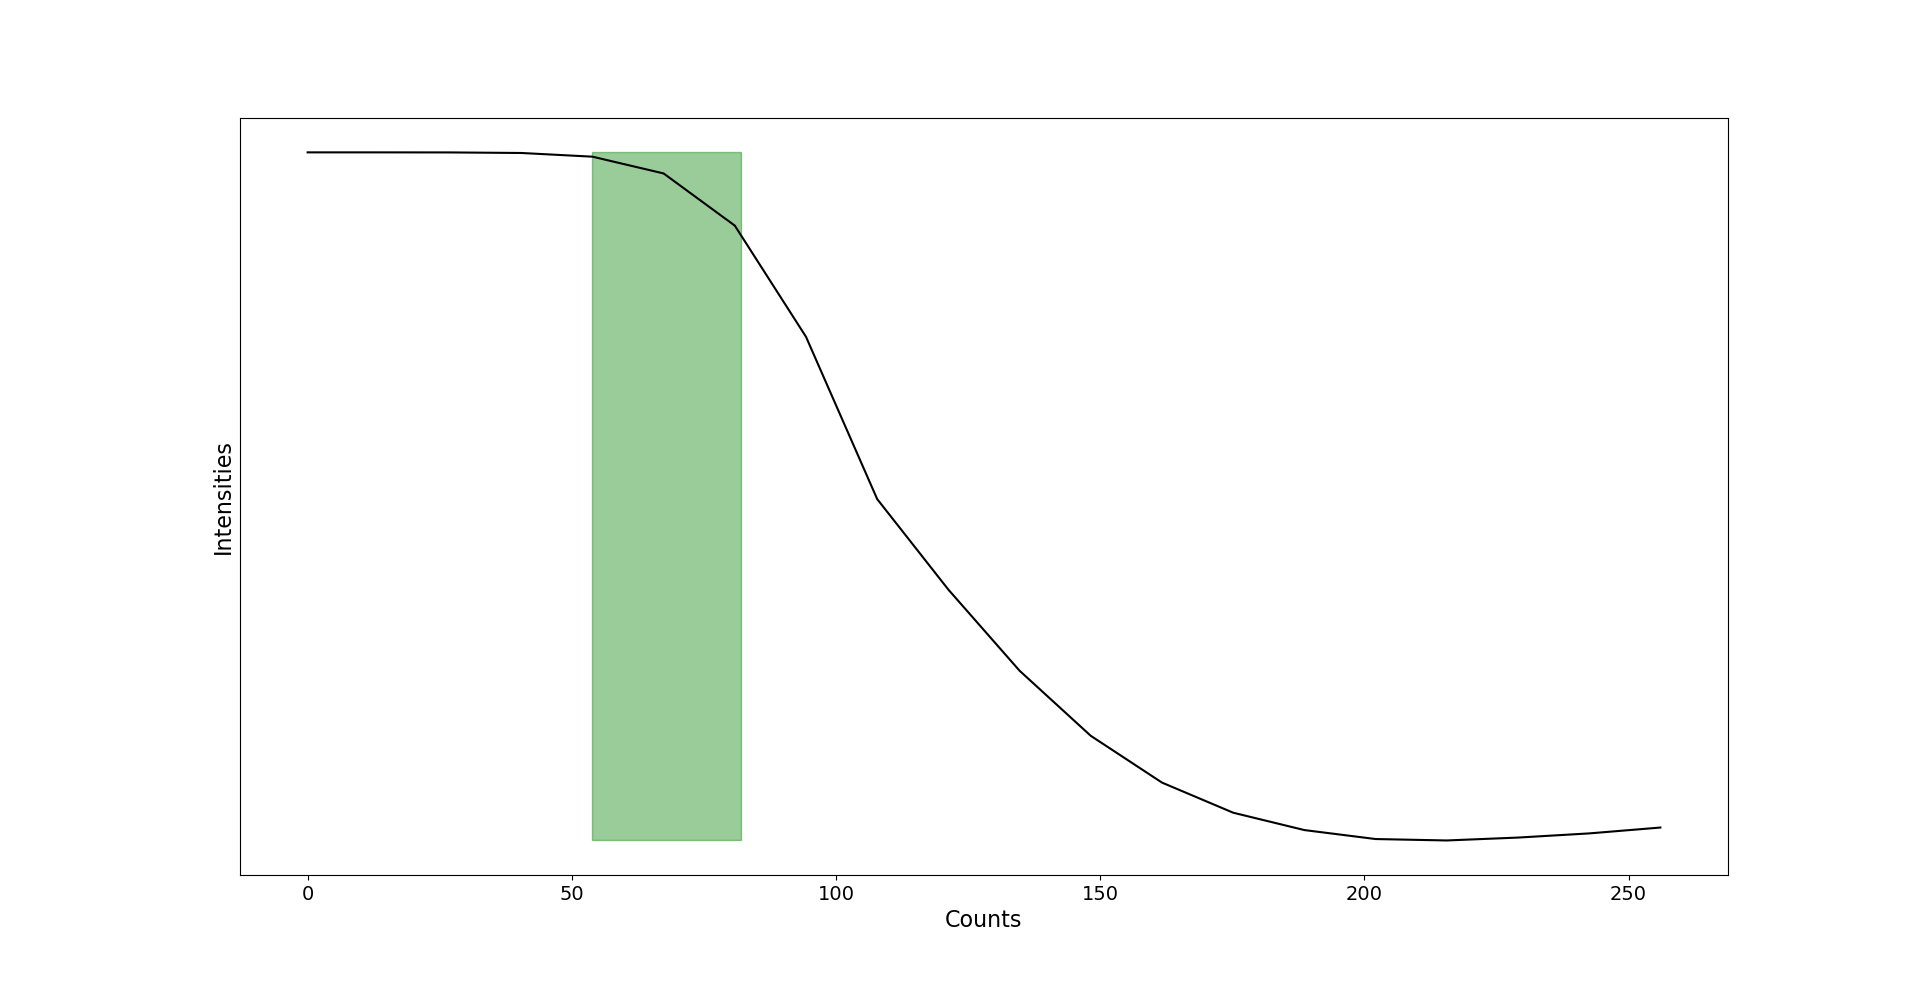
\includegraphics[width=0.49\textwidth]{figs/ch2figs/knees.png}}
    \subcaptionbox{Elbow example}{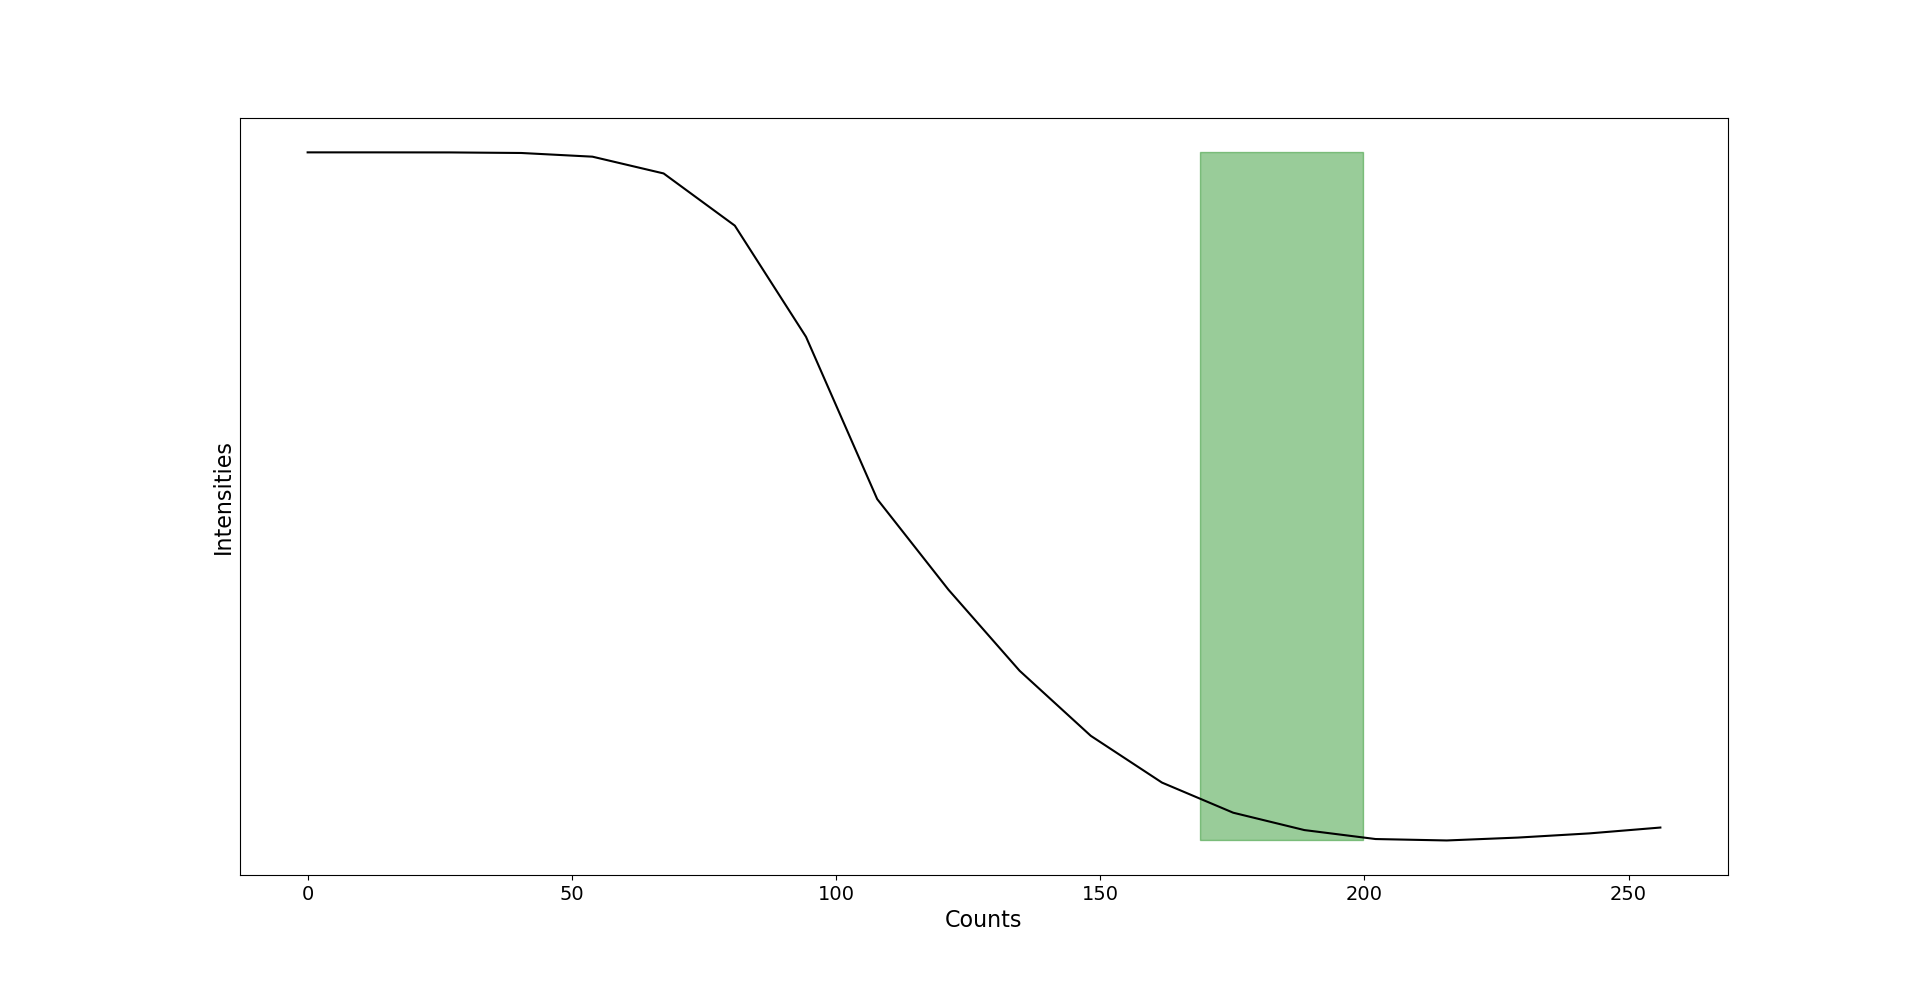
\includegraphics[width=0.49\textwidth]{figs/ch2figs/elbows.png}}
    \caption{Knee and elbow approximation regions are shown for some given distribution}
    \label{fig:knee_elbow_example}
\end{figure}
The method through which the Kneedle algorithm determines the knee points can be separated into six steps given some data set $D$ which is a finite discrete set of paired values $(x_i,y_i)$: 
\begin{enumerate}
    \item Smooth the discrete data set ($D$) to reduce the noise in the data. The retention of the shape of the set must be maximised.
    \item Normalize the finite data set points as the algorithm behaviour is independent of the point magnitudes. Both $x$ and $y$ values are normalized to a unit square while preserving their shape, as shown (Equation \ref{eq:smoothed_knee}):
    \begin{equation}\label{eq:smoothed_knee}
        \begin{split}
            D_{sn} &= \{(x_{sn},y_{sn})\},\text{ where}\\
            x_{sn_i} &= (x_{s_i}-min\{x_s\})/(max\{x_s\}-min\{x_s\})\\
            y_{sn_i} &= (y_{s_i}-min\{y_s\})/(max\{y_s\}-min\{y_s\})
        \end{split}
    \end{equation}
    \item A difference set ($D_d$) represents the differences between the $x-$ and $y-$value pairs which are mapped as ($x_{sn}, y_{sn}-x_{sn}$). This constructs a difference curve where the increases in the $y-$values are relative to the magnitude of the paired $x-$values. The insight provided by this difference curve is the behaviour it describes. When the curve transitions from horizontal to decreasing at a point indicates that said point is a potential knee.
    \item As mentioned prior, it is where the difference curve transitions from flattening to decreasing denoting the presence of a knee. Under the assumption that the points of the set are not decreasing, it is the local maxima of the difference curve that embody positions around which the rate of increase decreases noticeably. Each of these local maxima of the difference set is a candidate knee point.
    \item Each candidate knee occupies a local maxima where a certain deceleration in the smoothed data increase is perceived but the quantity of deceleration over a number of points defines what is declared as knees. At each candidate knee of the difference curve, a threshold value is calculated with a tunable sensitivity parameter ($S$). This threshold ($T_{lmx_i}$) is calculated by calculating the mean of the forward difference, with a spacing of 1, $(x_{sn_{i+1}}-x_{sn_i})$ which is multiplied by the sensitivity value ($S$) which is finally subtracted from the candidate knee value ($y_{lmx_i}$) for some candidate knee ($i$) shown in Equation \ref{eq:knee_threshold}.
    \begin{equation}\label{eq:knee_threshold}
        T_{lmx_i} = y_{lmx_i}-S\cdot \frac{\sum_{i=1}^{n-1}(x_{sn_{i+1}}-x_{sn_i})}{n-1}
    \end{equation}
    \item Each calculated threshold value is unique to each candidate knee (difference curve local maxima) and it is the decrease in the difference curve, after a candidate knee, relative to this threshold that determines whether it is a valid knee. The criteria are that the difference curve values, after a candidate knee, must decrease below the associated knee threshold ($y < T_{lmx_i}$) value prior to either increasing from a local minimum or encountering another candidate knee. If a local minimum of the difference curve is encountered, after which the curve increases, then the next candidate knee is evaluated. The smaller the sensitivity parameter ($S$) the closer the threshold to the candidate knee value (local maxima) and the easier it is to pass the criteria.
\end{enumerate}

\section{Prominent literature used in this research}
Throughout this chapter, various pieces of literature have been used in developing the system itself (detailed in Chapter \ref{ch:methodology}) or to develop an understanding of the biology and image processing that informed future decisions indirectly. For this breakdown, the literature will be separated by those that provided a foundational understanding of the fields involved with this research, those involved with the pre-processing of the image data prior to the thresholding system, and last will be the literature that was involved in the development of the automated thresholding system itself.
\subsection*{Foundational understanding}
\paragraph{Biology} The foundation of this came from a high-level understanding of the biological phenomena that describe the organelles of interest and the mitophagy process which is the process that will be analyzed after complete pre-processing. The largest contributor to understanding mitophagy and the related organelles was \textit{Human Physiology: From Cells to Systems}~\cite{cell_phys_book} which covered information regarding autophagy, the mitochondria and, to a lesser degree, mitophagy. More detailed information relating to autophagosomes, lysosomes and the relationship between the two is detailed in \textit{The discovery of lysosomes and autophagy}~\cite{lyso_auto_relation}. Detailed insight on mitophagy and its relationship with the fission and fusion of mitochondria is covered in \textit{Mitochondrial fission, fusion, and stress}~\cite{MitoFus-2012} and \textit{Mechanisms of mitophagy}~\cite{MitoMechan}. \paragraph{Microscopy} The fundamentals provided by microscopy are to recognise the causes of reduced image quality or errant phenomena observed that originate from the imaging process. A particular impact on this understanding of confocal microscopy is \textit{Fluorescence microscopy}~\cite{Sanderson-2014} but it is the constraints listed as bleed-through, photobleaching and diffraction that are the most valuable as these understanding of these constraints can inform undesired behaviours or details seen in the image during the analysis that might not relate to the actual specimen. Bleed-through was detailed by \textit{Fluorescence microscopy}~\cite{Sanderson-2014} and \textit{A guided tour into subcellular colocalization analysis in light
microscopy}~\cite{Bolte-2006}; photobleaching was informed by \textit{Photobleaching kinetics of fluorescein in
quantitative fluorescence microscopy}~\cite{photobleach_excite} and \textit{Loss of image quality in photobleaching
during microscopic imaging of fluorescent probes bound to chromatin}~\cite{photobleachingPaper}; and diffraction was informed by \textit{Diffraction-unlimited optical microscopy}~\cite{Diffraction_Patterson} and \textit{ Diffraction-unlimited optical microscopy}~\cite{Diffraction_Dedecker}.

\subsection*{Pre-processing understanding}
Since this research is exploring and developing an automated high-throughput thresholding system it is important to understand other pre-processing techniques that are applied to the image prior to the application of the system. Likewise understanding the influence of these techniques regarding the manner in which they improve image quality (noise removal, signal enhancement, etc.) is crucial as each of these methods can impart an undue effect on the image as a byproduct of their process and mitigate these byproducts using subsequent pre-processing techniques, including the automated thresholding. An overview of deconvolution, the generation of the PSF, and a high-level mathematical representation of the diffraction effect and its removal via deconvolution is described by \textit{3D PSF models for fluorescence microscopy in ImageJ}~\cite{psfgen} for the generation of synthetic PSFs, and by both \textit{Blind deconvolution of gaussian blurred images containing additive
white gaussian noise}~\cite{6505824} and \textit{Deconvolutionlab2: An open-source software for deconvolution microscopy}~\cite{DeconLab2} in terms of the mathematical representation. For denoising, a statistical understanding of noise (not artefacts or bleed-through) is provided by \textit{Analyzing fluorescence microscopy images with ImageJ}~\cite{bioimage_book} while the behaviour of standard denoising filters is informed by median and Gaussian filters but also by the Sigma filter~\cite{sigma_filter}. For image enhancement, the primary insight developed was through analysis of two such methods for background subtraction and contrast enhancement described by \textit{Biomedical image processing}~\cite{rolling_ball} and \textit{Contrast Limited Adaptive Histogram Equalization}~\cite{clahe} respectively. The last group of methods were those relating to thresholding which is separated into global and local methods that segment the image into foreground and background thus binarizing it. Thresholding as a whole was described by \textit{Chapter 9 - image segmentation}~\cite{segmentation_book} in the context of image segmentation while further detail regarding global and local methods was informed by \cite{Otsu1979ATS} and \textit{Analyzing fluorescence microscopy images with ImageJ}~\cite{bioimage_book}. These pre-processing methods were all to be applied sequentially within a pipeline and a paper which stimulated the exploration into why these methods are applied sequentially was provided by \textit{A pipeline for multidimensional confocal analysis of
mitochondrial morphology, function, and dynamics in pancreatic $\beta$-cells}~\cite{PipelineDecon-Chaudhry}.

\subsection*{Literature that directly impacted system design}
The research that directly featured in the automated thresholding system being developed or that was compared against for evaluation consists of a number of thresholding techniques and other algorithms. These thresholding techniques are the Otsu threshold~\cite{Otsu1979ATS}) and Triangle threshold~\cite{triangleThresh} as they are both automated threshold methods reliant on image histogram being bimodal or close to. Hysteresis thresholding, proposed by \cite{Hysteresis}, is important as it forms the backbone of the system design while the Kneedle algorithm~\cite{kneedle_paper} is an unconventional approach for low threshold approximation detailed in Chapter \ref{ch:methodology}.  

\section{Chapter conclusions}
%This chapter conveys a body of information providing context behind choices made throughout this project. Some of these choices were determined externally by the mitophagy research application case of this project while others were design decisions made during the development of the high-throughput thresholding system. References to the information covered in this section will be made in Chapter 3 where other research related to cellular microscopy thresholding, subcellular microscopy thresholding and automatic thresholding are explored. Chapter 4 describes two main components with the first relating to the image acquisition and processing prior to the thresholding system application and the second being the design of the thresholding system.  

This chapter conveyed theory and concepts relating to the techniques that will be implemented or are to be explored throughout this work. This theory extended from providing context around the approaches dictated by the mitophagy research use case to those being explored for implementation in the high-throughput thresholding system design. The mitophagy research use case determines the objects to be imaged (Section \ref{sec:mito_detail}), the microscopy technique to be used (Section \ref{sec:fluorMicr}), and the analysis approach (colocalisation) that the images must be of suitable quality for (Section \ref{sec:coloc}).\par The thresholding system being designed is not expected to function in isolation with a number of adjacent approaches applied before or after the system to maximise the restored image quality. For this reason, the context was provided regarding factors of image quality degradation (Section \ref{sec:Noises}), a high-level overview of the sequential application of approaches to improve the image quality (Section \ref{subsec:pipe}), and a high-level overview of these approaches grouping them by the aspect of image quality that is addressed (Section \ref{sec:overview_preproc_methods}). There is also a deeper discussion on the theory surrounding specific approaches of interest to this work (Section \ref{sec:further_methods}).\par This chapter serves to consolidate and organise all of the theoretical backgrounds of phenomena, techniques and approaches that inform design choices and observed behaviours of the high-throughput thresholding system. The proceeding chapters (Chapter \ref{ch:methodology} and Chapter \ref{ch:results}) both reference this chapter in terms of both the specimens and imaging techniques used for image acquisition, and the techniques implemented in the system design to develop a high-throughput thresholding system. 
 
\chapter{Methodology}\label{ch:methodology}
% This section will describe the data used (in terms of it's properties such as wavelengths z-steps, timelapse lengths (if consistent), the source of the cell cultures and the make of the microscope used) and why the data was collected in this way (confocal for 3D resolution, treatments applied for mitophagy). Section for methodology employed for auto thresholding

With Chapter \ref{chp:Background} providing background context for the 
\section{Dataset acquisition process and preparation}\label{sec:Dataset_making}
%this section describes properties surrounding the data acquisition, structures labelled (organelles), the fluorophores used, the treatments applied and concisely why, the reason for confocal microscopy (3D resolution and reduced out-of-focus fluorescence), and imaging parameters such as z-step size etc. such that someone could hypothetically reproduce this.
The image data set that was acquired for this research project is composed of microscopy images that can be used in mitophagy analysis. This is due to the primary intended application of this automated binarization system being in the high-throughput pre-processing of microscopy images in mitophagy research.
\subsection{Sample preparation prior to imaging}
%This subsection must discuss what cell types were used, the treatments applied, the organelles stained and the reasons (briefly)
\subsubsection*{Cell culturing}
MEF and GT1-7 cell lines were used and were maintained in Dulbecco's Modified Eagle Medium (DMEM) (ThermoFisher, \#41965062) supplemented with 10\% fetal bovine serum (FBS) (Sigma-Aldrich, \#F0679) and 1\% Penstrep (Sigma-Aldrich, \#P4333) and were kept in a humidified incubator at 37$^{\circ}$C and 5\% CO2. Cells were subcultured using trypsin (Sigma-Aldrich, \#T4049) to detach cells from flasks. Afterwards, DMEM was added to the cells at a 2:1 ratio and cells were collected into 15 mL Falcon tubes (Bio-Smart Scientific, \#50050). Cells were centrifuged at 1500 rpm at room temperature for 3 minutes (Centrifuge, Eppendorf, \#5804R). Media was discarded and cells were resuspended in fresh DMEM. Cells were seeded to T25 flasks (Bio-Smart Scientific, \#70025) 8-chamber dished (ThermoFisher, \#Z734853).
\subsubsection*{Treatments applied}
All treatment interventions were made up using 1x phosphate-buffered saline. The treatments applied were memantine hydrochloride (Sigma-Aldrich, \#PHR1886), carbonyl cyanide m-chlorophenylhydrazone (CCCP) (Sigma-Aldrich, \#857815), and bafilomycin A1 (Baf) (Sigma-Aldich, \#B1793). Only the GT1-7 cells were treated with Memantine hydrochloride which was done by incubating the treatment with the cells at working concentrations of either 50 $\mu$M (LM) or 100 $\mu$M (HM), low and high concentration dosage respectively, for 48 hours prior to any imaging and while refreshing any memantine-treated media every 24 hours. The CCCP treatment was incubated 6 hours prior to imaging at 10 $\mu$M causing mitochondrial depolarization with the goal of increasing the frequency of mitophagy events to observe them. The Baf treatment was incubated with the cells 4 hours prior to imaging at 400 nM to inhibit the completion of mitophagy by preventing the fusion of lysosomes and autophagosomes (described in Section \ref{subsec:lysosome}) resulting in damaged mitochondria to remain contained in autophagosomes. Different combinations of these treatments formed treatment groups, with no treatments forming a control group, so that observations from the analysis could be better correlated with the appropriate treatments.
\textcolor{red}{I feel that this, due to being basically copied from Sholto, should reference the same paper in case it is flagged for plagiarism}
\subsection{Image acquisition via microscopy}
%Briefly discuss the resolution used, the fluorophores in terms of cross-talk, the z-resolution ranges, the z-step size, the microscopy used (confocal) and the type of microscope used such that these imaging conditions can be reproduced.
The mitochondria, autophagosomes, and lysosomes were imaged for the image data set used in this research as they are the organelles associated with mitophagy. To image these intra-cellular organelles with specificity and easy differentiation confocal microscopy was used as fluorophores can be selected specific to the organelles of interest. The imaging was performed using a Carl Zeiss LSM780 ELYRA PS.1 Super-resolution platform using an LCI Plan Apochromat 100x/1.4 Oil DIC M27 objective at 100x magnification with the lateral slices composing the 3D z-stack having a step-size of 0.35 $\mu$m between each slice with the number of slices ranging from 6 to 13 depending on the sample.\par 
Green fluorescent protein - light chain 3 (GFP-LC3) plasmid (Addgene, \#21073), LysoTracker Red (ThermoFisher, \#L7528), and MitoTracker DeepRed (ThermoFisher, \#M22426) were used to fluorescently stain for autophagosomes. lysosomes and mitochondria respectively. For GFP-LC3, 5 $\mu$g were transfected into the cells using the NEON Electroporation System (Invitrogen, MPK5000) and NEON Transfection tool kit (Invitrogen, MPK10096) according to the manufacturer's instructions. These transfected cells were seeded onto 8-chamber dishes 24 hours before the treatment protocol. The LysoTracker Red and MitoTracker DeepRed were combined into a master mix solution at 75 nM each and were incubated with the cells for 20 minutes prior to imaging. The GFP, Lysotracker and Mitotracker used were excited during fluorescence microscopy by lasers with a wavelength of 488nm, 561 nm and 633 nm respectively with 561 nm and 633 nm kept on separate tracks to avoid cross-talk and bleed-through between them. 

\subsection{Preprocessing prior to thresholding}\label{sec:preprocess_applied}
After the cell images have been acquired they are pre-processed to improve the image quality before any analysis is undertaken. The pre-processing pipeline that was implemented entailed:
\begin{enumerate}
    \item Deconvolution: Richardson-Lucy Total Variation (RLTV) Deconvolution~\cite{DeconLab2, rltv}
    \item Upscaling: Bicubic interpolation
    \item Background subtraction: Rolling ball algorithm~\cite{rolling_ball}
    \item Denoising: Sigma filter plus~\cite{sigma_filter}
    \item Image enhancement: Contrast Limited Adaptive Histogram Equalisation (CLAHE)~\cite{clahe}
    \item Gamma correction
\end{enumerate}
For each image in the batch the number of lateral z-slices (z-resolution), the NA, the channel wavelength, the refractive index immersion, the pixel resolution, the pixel size and z-step size would be used to generate a theoretical PSF for the said channel using software~\cite{psfgen}. Since the channels were associated with specific fluorophores and all other parameters, except for the z-resolution (z-stack size), the PSF could be generated prior and applied to all images matching those parameters.\par With the PSF generated deconvolution is performed using a FiJi~\cite{Fiji_paper} plugin called DeconvolutionLab2~\cite{DeconLab2} and the applied techniques is RLTV~\cite{rltv}. This differs from the Richardson-Lucy deconvolution described prior (Section \ref{subsec:richardson_lucy}) where the addition of the total variation regularization reduces noise amplification while still preserving the edges of objects. Bicubic interpolation is used to upscale the deconvolved image prior to further processing. Once upscaled, background subtraction is applied to correct any uneven illumination that may be present in the image followed by denoising. With the illumination balanced throughout the image, the sigma filter can be applied to remove noise. This filter is similar to a mean filter which is with the added benefit of better edge preservation and robustness to outliers within the pixel neighbourhood. Image enhancement through CLAHE is applied which compensates for some of the signal loss due to denoising and the localised application of it to pixel neighbourhoods means that the contrast enhancement is adapted to the specific pixel regions. This results in a contrast adjustment that is not sensitive to localised fluctuations in the contrast providing a better end result given that the parameters are suitable for the image. Lastly, gamma correction is applied to the image and is typically followed by binarization to produce a mask of the objects of interest depending on the analysis. Since this research project entails the development of a binarized mask designating the foreground and background objects in the image all images will be pre-processed as described above.
\section{Automatic thresholding method}
%First start with a preface regarding the structuring of this method and how it was born (to automate thresholding that could threshold images consistently with a sufficient degree of accuracy)
In order to achieve the objectives discussed in Section \ref{sec:objectives}, a new image binarization method was developed. Initially, both automated global and local thresholding methods were experimented with where it was heuristically determined that each had caveats preventing them from meeting these objectives. While automated global thresholding methods require no mandatory parameter selections the results achieved are highly sensitive to both the imaging conditions and the image quality. Automated local thresholding methods are more robust to image quality due to the ability to evaluate the threshold based on pixel attributes that are significant in localized regions (such as the contrast of an object edge) but are dependent on the correct parameter selection and tuning to produce optimal results. Due to this a new method was developed with the intent of adopting the benefits of each of both global and local being the lack of parameter tuning and the robustness to poor image quality.
\iffalse
The automatic thresholding method was developed with the intention of providing image thresholds with minimal or no human involvement. The requirements of this method were to provided threshold results that are usable in further analysis or processing with a quality comparable to or exceeding that of a novice image analyst and to threshold large batches of image with consistent results.
\fi
\subsection{Choice of threshold method} \label{sec:thresh_choice}
%This subsection must describe why Hysteresis thresholding was chosen as the thresholding method as opposed to others. Refer to chapter 2
Rather than attempt to establish an entirely new binarization method the improvement of an established method was deemed prudent. Since such a method would have already been tested prior benefits and drawbacks of such a method were already known and could potentially be addressed through this method. \paragraph{Hysteresis thresholding}(Section \ref{sec:Hyst}) was chosen as the results were similar to that of local thresholding methods where the outcome was the intensity of pixels (or voxels) within an object where considered and allowed individual objects to be validated. This was also similar to global thresholding methods as the parameters to be selected were intensities which could be inferred from the image histogram or be determined by other image intensity-based criteria. While methods like Adaptive Thresholding may provide more robust results, the necessity of visual analysis in the approximation of the parameters including the tuning of said parameters makes it, along with most other automated local thresholding methods, either inappropriate or less appropriate for automated high-throughput thresholding. Using the showcase of the Hysteresis application in Figure \ref{fig:hysteresis_showcase_2D_3D}, an analogy can be presented to both summarize the logic behind Hysteresis thresholding and the role each parameter plays in it. Assume that the pixels of the image described a terrain composed of a landmass with heights relative to the pixel intensities displayed in Figure \ref{subfig:raw_3D}. Certain regions of this landmass are of interest typically those that would be islands possessing mountains of a certain height. The sea level and mountain threshold are each visualised by a \#blue and \#yellow plane respectively where regions of land above the `water' are considered independent regions, or continuous contours, with each being a potential island of interest as seen in Figure \ref{subfig:hyst_labels_3D}. Islands that intersect with the \#yellow plane are those that can be deemed to be mountains and said islands are then deemed to be of interest. A representation of this selection can be shown in Figure \ref{subfig:hyst_applied_3D} where only the islands meeting said criteria remain. In this analogy, the sea level represented the low threshold, the mountain height threshold represented the high threshold while the continuous regions above the low threshold represented potential foreground regions. \paragraph{Considerations due to this} were determined early in the system prototyping when postulations regarding how image properties or behaviours could be related to the thresholding and be quantified using an algorithm removing human involvement. This is performed in automated local thresholding methods like Sauvola~\cite{adapt_sauvola} where a number of parameters can be left as their defaults but these only function well under specific circumstances and can collapse if the image differs too much from the image around which the defaults were approximated. A number of these methods were used earlier for pre-processing and it was 
developed method was to be a medium built upon Hysteresis thresholding and what components of Hysteresis thresholding could be addressed through this method. The primary components are the binarization logic the method employs and the parameters which need to be selected to execute this logic which typically involve some level of visual analysis to approximate appropriate parameters. It is the latter component is the parameter selection which prevents high-throughput application yet provides most of the robustness as the low and high thresholds can be tuned to reduce the impact of image degradation on the binarization result.\paragraph{The system design based on this} will target the determination parameter selection in a manner that is both automatic and adapts to each image by allowing them to be automatically "tuned" to each image by considering features related to the image pixel intensities. Based on the analogy described prior, the low threshold must first be acquired as it determines what pixels compose potential foreground regions while the acquisition of the high threshold will follow to filter which of said regions actually belong to the image foreground.
\begin{figure}
%This will be a figure made with 6 subfigure panels. The left-hand panels will be the 2D versions while the right will be the 3D. The first pair will be the raw image, the second will be with the thresholds highlighted (the 2D will highlight structures if above or below the thresh), and the third pair will be post thresholding.
    \centering
    \subcaptionbox{2D representation of the image prior to any threshold application \label{subfig:raw_2D}}{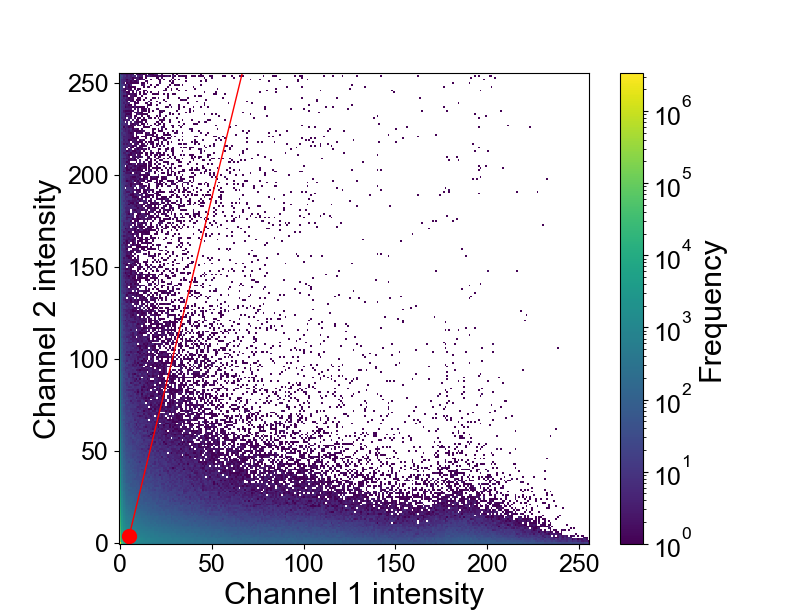
\includegraphics[width=0.49\linewidth]{figs/Placeholder_Image.png}}
    \subcaptionbox{The 3D intensity elevation projection of the image where the z-axis heights represent the pixel intensities \label{subfig:raw_3D}}{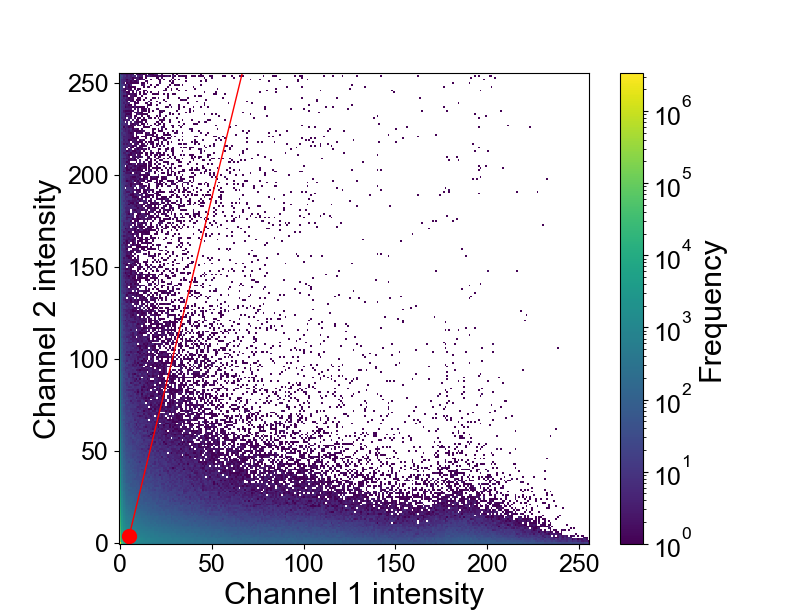
\includegraphics[width=0.49\linewidth]{figs/Placeholder_Image.png}}
    \subcaptionbox{The 2D image with the objects above and below the thresholds labelled. \label{subfig:hyst_labels_2D}}{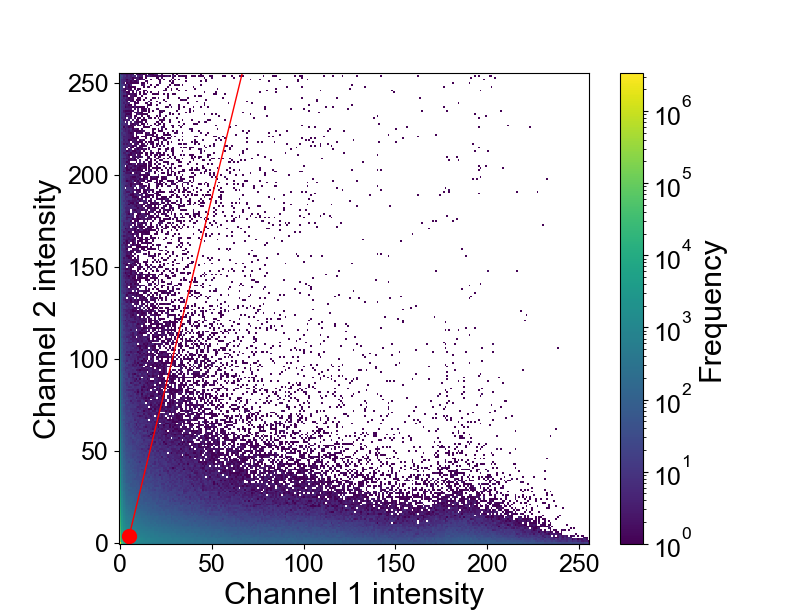
\includegraphics[width=0.49\linewidth]{figs/Placeholder_Image.png}}
    \subcaptionbox{The 3D representation with coloured labelling based on the thresholds \label{subfig:hyst_labels_3D}}{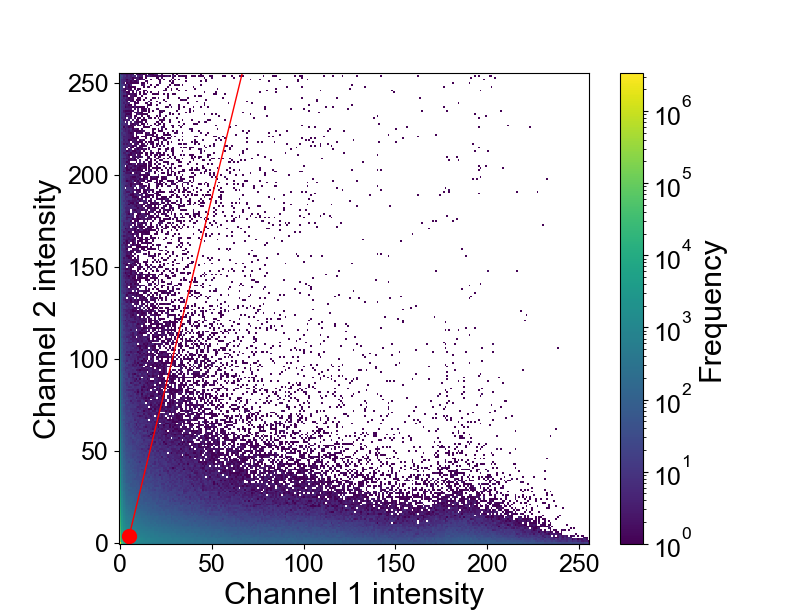
\includegraphics[width=0.49\linewidth]{figs/Placeholder_Image.png}}
    \subcaptionbox{The binarized 2D image of the regions that are preserved after Hysteresis is applied \label{subfig:hyst_applied_2D}}{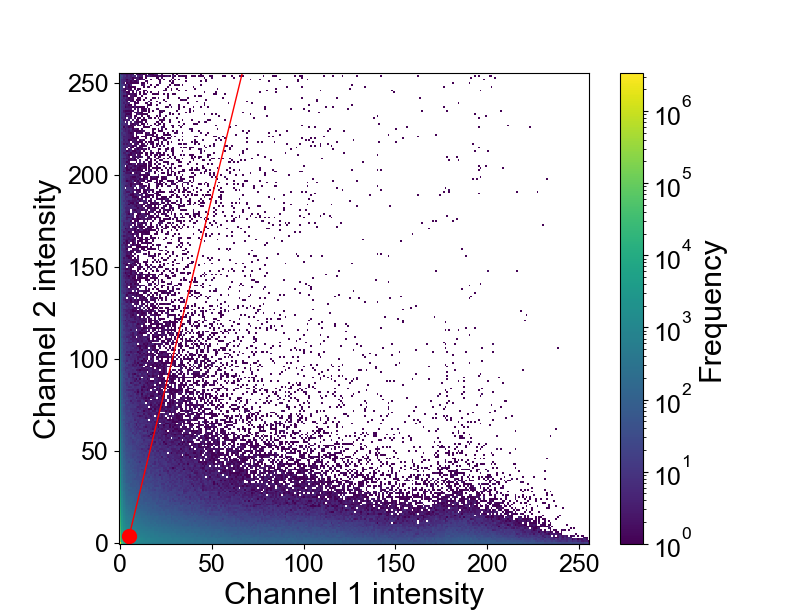
\includegraphics[width=0.49\linewidth]{figs/Placeholder_Image.png}}
    \subcaptionbox{The 3D intensity projection of the image after Hysteresis is applied. \label{subfig:hyst_applied_3D}}{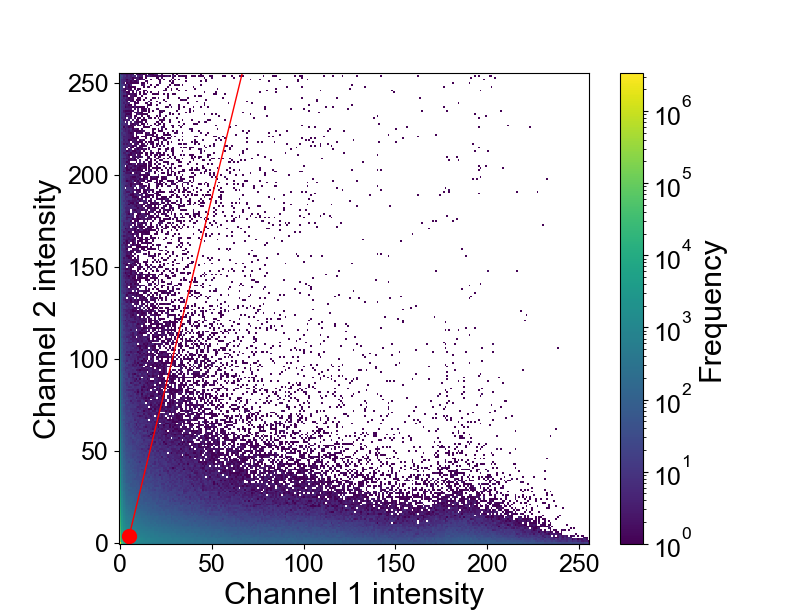
\includegraphics[width=0.49\linewidth]{figs/Placeholder_Image.png}}
    \caption[\textcolor{red}{This is currently not complete as 3D images are being a bit difficult and this is going to be moved to Chapter 2 (Hysteresis Section)}Showcasing the application of Hysteresis thresholding on a microscope image along with 3D intensity projections]{The application of Hysteresis thresholding is illustrating using an arbitrary 2D microscope image which is shown in sub-figures (\subref{subfig:raw_2D}), (\subref{subfig:hyst_labels_2D}), and (\subref{subfig:hyst_applied_2D}) while the 3D representation of each of these sub-figures are shown in (\subref{subfig:raw_3D}), (\subref{subfig:hyst_labels_3D}), and (\subref{subfig:hyst_applied_3D}) respectively. The Hysteresis labels applied in sub-figures (\subref{subfig:hyst_labels_2D}) and (\subref{subfig:hyst_labels_3D}) are selected based on what the pixel intensity is relative to the low and high thresholds with red representing pixels above the high threshold, green representing pixels between both thresholds and green representing pixels below the low threshold. Sub-figures (\subref{subfig:hyst_applied_2D}) and (\subref{subfig:hyst_applied_3D}) show the image after Hysteresis application with the results being binarized in the 2D representation (\subref{subfig:hyst_applied_2D}) while the 3D representation (\subref{subfig:hyst_applied_3D}) uses the binary output to mask the intensity image to improve clarity.}
    \label{fig:hysteresis_showcase_2D_3D}
\end{figure}
\subsection{Acquisition of the low threshold}\label{sec:low_acquis}
%Describe use of Kneedle (which should be discussed in theory in Chapter 2) and cite the github used for the software implementation. The use of the Normal and Log version (need to confirm that the log knee is always greater than the normal knee using data), and how Otsu is used to select the low threshold (picking between normal and log knee and compare both with Otsu thresh for why Otsu isn't used).
As has been described in Section \ref{sec:Hyst}, the low threshold is a crucial step in determining the quality of the Hysteresis thresholding outcome since it is the first threshold value deciding which voxels are background. This is important as the high threshold only acts on the remaining non-background voxels in the image thus a low threshold that is too low or too high results in either image noise that increases the difficulty of the high threshold selection or removes valuable regions of objects. Despite this, thresholding is a subjective operation frequently relying on the judgement of an expert to evaluate what is currently designated as background voxels in the image and whether they belong to an object of interest to the analysis.
\subsubsection*{Initial steps}
In the beginning, an investigation into robust and accurate low threshold estimators was performed but it was found that the established methods were lacking and for this reason established automated global threshold methods were considered. Automated global threshold methods had the benefit of not requiring parameter setting or tuning (aligning with a design objective of the system this research was developing) and there was a robust body of literature on these methods regarding their development. Many of these methods also were implemented in Python libraries thus the methods `Li', `Mean', `Otsu', `Triangle', and `Yen'~\cite{scikit-image} were tested. These methods were tested by application to the 25 sample images with the threshold results compared to the low threshold values selected by the experts.\paragraph{Initial findings} were that values chosen by `Li' or `Mean' were often far lower than the experts while `Yen' resulted in threshold values that diverged so greatly from all of the experts that Yen was omitted from further testing. Despite thresholding being a subjective evaluation, as mentioned prior, it is still ideal to achieve a closer value to the experts although how close, unfortunately, is image dependent. The remaining two methods, `Otsu' and `Triangle', were generally closer to the expert values although Otsu was generally closer to the experts.
%as can be seen in Table \ref{tab:results}.
\textcolor{red}{The table is empty for now as I need to determine if formatting functions well for horizontally long tables using tikz or tabular. For now, this is a placeholder and the boxplots visually describe this better (perhaps this should be moved to appendices?)}
\iffalse
\begin{table}
%A placeholder. If the sample data is too wide then the table will be generated as an image and then inserted. For now this will be where low threshold results will sit.
\begin{center}
\begin{tabular}{ |c|c|c| } 
 \hline
 cell1 & cell2 & cell3 \\ 
 cell4 & cell5 & cell6 \\ 
 cell7 & cell8 & cell9 \\ 
 \hline
\end{tabular}
\end{center}
\caption{\textcolor{red}{This is currently still a placeholder as I am determining a) if the formatting will work for the full numeric results; and b) whether they should rather be moved to the appendices as the box plot explains it better}\label{tab:results}}
\end{table}
\fi
This is visually described in Figure \ref{fig:expert_boxplot} where the overlaid box plot and strip plots represent the difference between each thresholding method and the experts for each sample. Although this is not a perfect comparison as each sample is technically unique to each other and this comparison is reductionist in that it does not consider the conditions of each image that lead to certain results but this can serve as an estimation of the sensitivity of the performance of the thresholding methods and how robust they are to a range of image conditions. As these comparisons regard the difference between the threshold method and the expert results tending towards zero are better as they are more similar to the expert with Figures \ref{subfig:thresh_diff} and \ref{subfig:vox_diff} describing the difference between the threshold value and the number of foreground voxels respectively. Although it was already established that Otsu and Triangle were the best-performing threshold methods there is confirmation of this with the threshold value difference (Fig. \ref{subfig:thresh_diff}) where Otsu has larger quartile ranges than that of Triangle but with the distribution of sample values more closely centred on the zero line. What this means is that Otsu experiences greater swing in performance across samples yet when it does perform well it performs better that Triangle yet Triangle is more consistent in outcome although this outcome is slightly worse. Image thresholding remains a highly subjective and image-dependent evaluation and for this reason, although still an unsatisfactory measure of overall performance, an evaluation in the binarization output per sample (Fig. \ref{subfig:vox_diff}) is to be explored. This difference in foreground voxel counts shows that save for Expert A, Otsu has greater consistent similarity to the experts although the shortcoming is that when it deviates it can deviate strongly. When this analysis was conducted there was also an evaluation of the binarization outcome on the samples between the thresholding methods and the experts although only these reductive comparisons have been shown as they serve as effective approximations of the binarization results across a large body of samples. What was determined is that although these methods could provide passable results, the impact of poorly selected low thresholds can render a binarization outcome useless for analysis, if not detrimental if uncaught, thus an alternative thresholding method is required.
\begin{figure}
    \centering
    \subcaptionbox{Difference between the low threshold determined by the automated method and the experts\label{subfig:thresh_diff}}{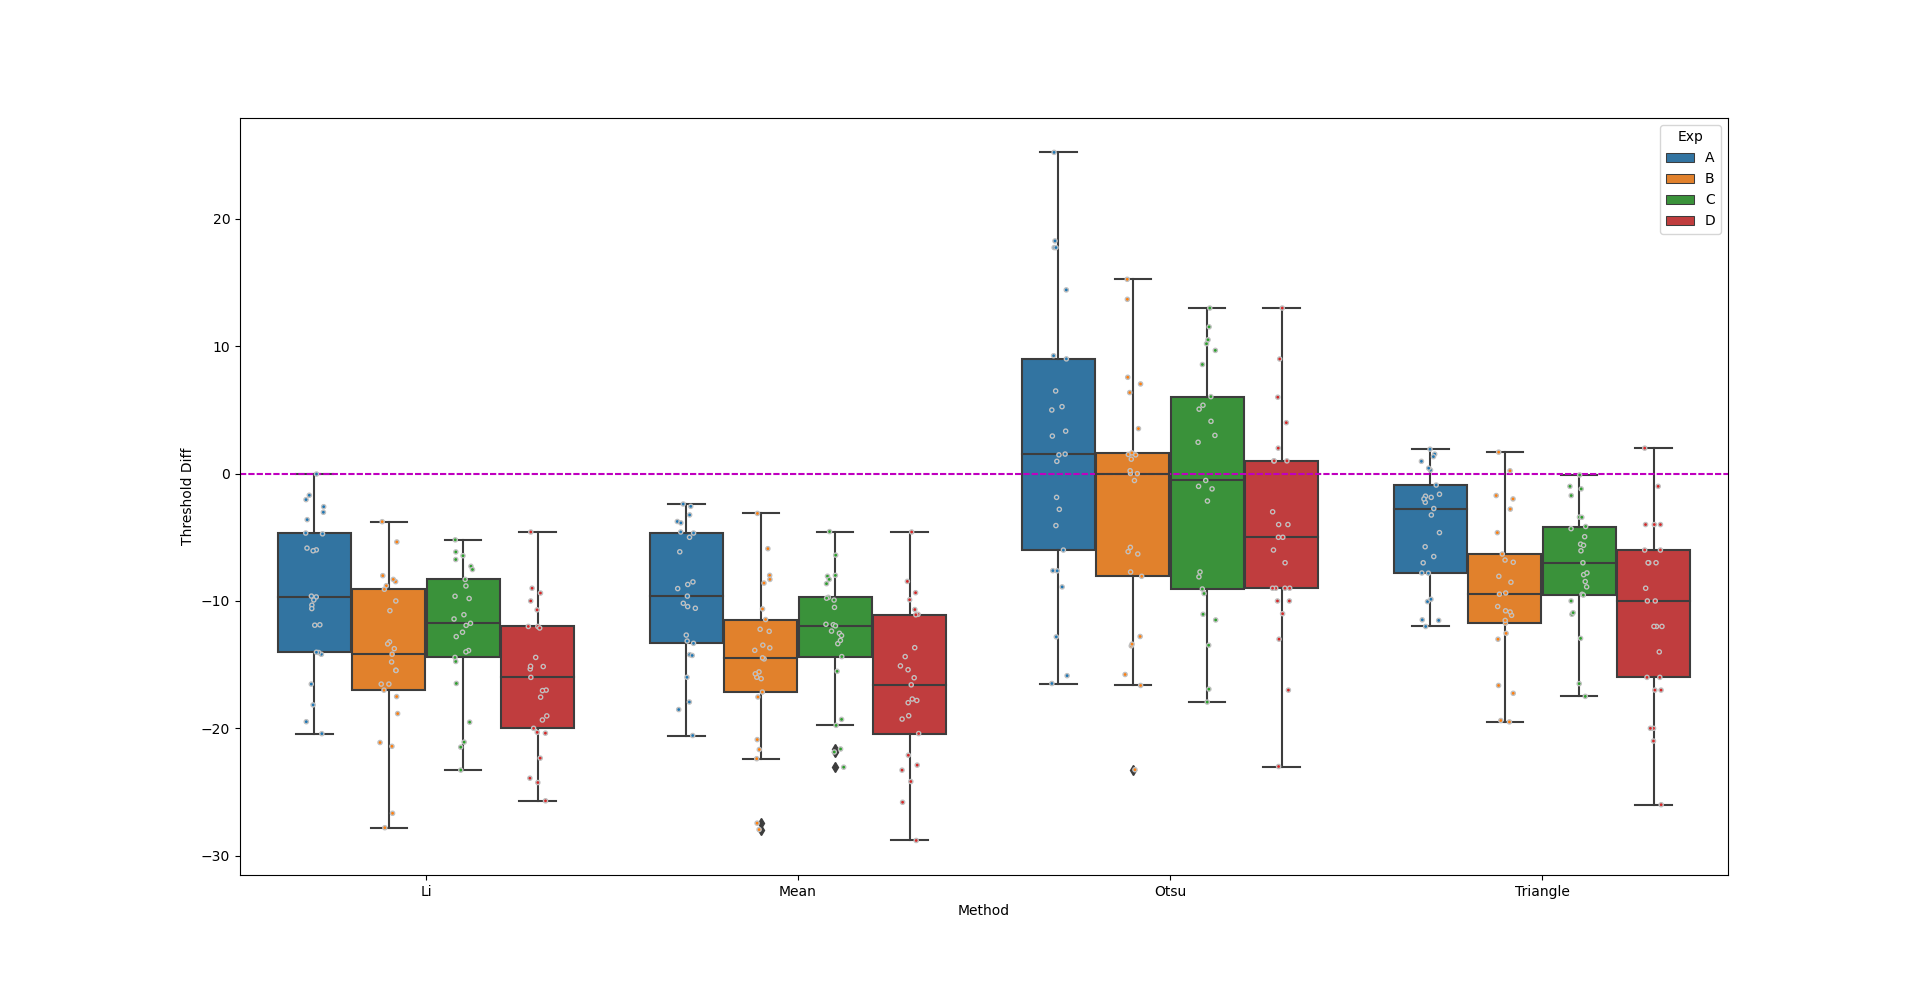
\includegraphics[width=\textwidth]{figs/ch3figs/Thresh_diff.png}}
    \subcaptionbox{Difference in non-background voxel count between the automated methods and the experts\label{subfig:vox_diff}}{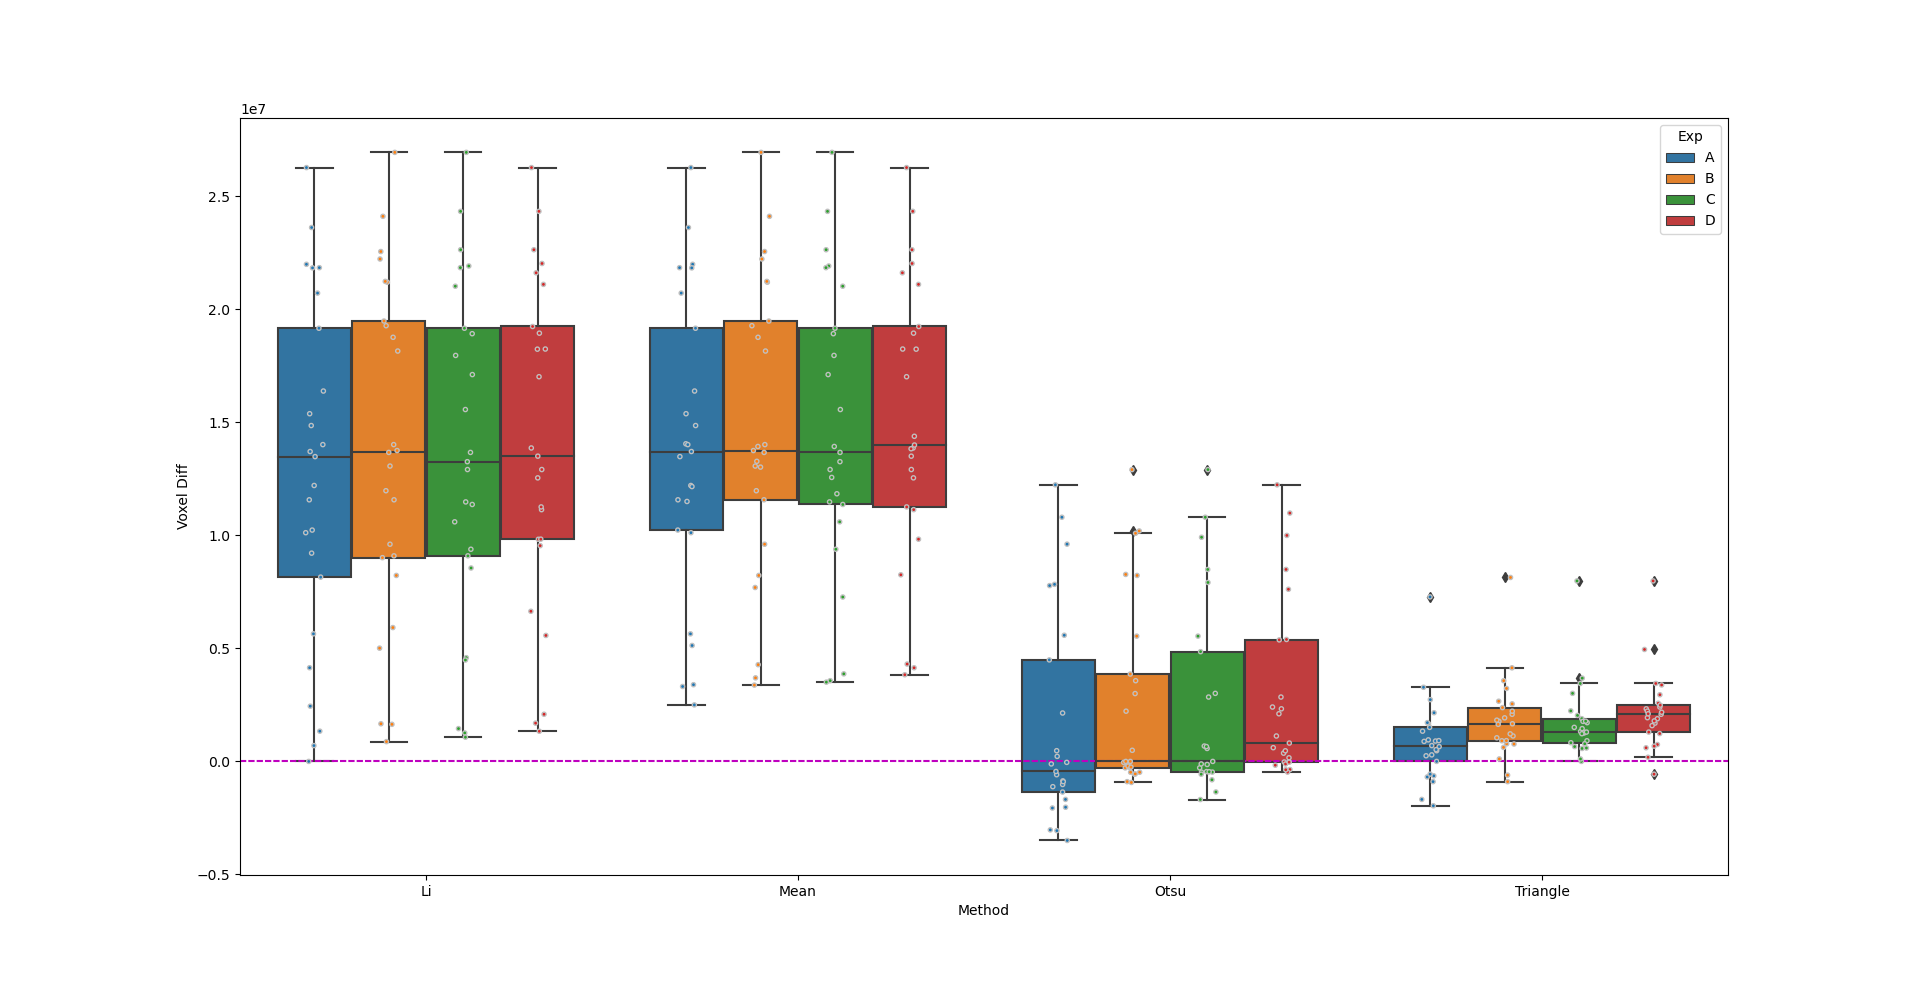
\includegraphics[width=\textwidth]{figs/ch3figs/Vox_diff.png}}
    
    \caption[Difference between expert values and automated thresholding results in terms of the threshold value and binarization outcome]{Difference between expert values and automated thresholding results in terms of the threshold value and binarization outcome depicted using box plots overlaid with strip plots. These plots describe the difference between the thresholding method and the experts for each sample where (\subref{subfig:thresh_diff}) represents the difference in the numeric threshold value while (\subref{subfig:vox_diff}) represents the difference in the count of the foreground image pixels. As greater similarity is preferred the goal is a value of zero denoted by a dashed magenta line on both sets of plots.}
    %Caption needs to be improved
    \label{fig:expert_boxplot}
\end{figure}
\paragraph{The alternative} thresholding method that was decided on was an application of the `Kneedle' algorithm (Section \ref{sec:kneedle}) where elbows within the image histogram are to be used as the low threshold. The motivation for this decision was based on comparisons between the expert-selected low thresholds and where they are positioned on the image histogram as it was hypothesised that there is some low-intensity region of the histogram that would represent the image background. The challenge surrounding this was, once again, that image binarization is a subjective process where typically some value can be estimated and based on its impact on the binarization it is further tuned. Despite this, it was hypothesised that there must be some baseline which would generally be agreed upon by experts regardless of the results. This baseline was formulated from four notions being:
\begin{enumerate}
    \item That there will always be a background within the image, as there must be two states to differentiate between with binarization, where the background will be comprised of voxels with intensities ranging from the lowest in the image up to, or below, the lowest foreground intensity.
    \item While the upper bound of the background intensity range is uncertain initially, the lower bound is well-defined. Given this, there is complete certainty that the lowest intensity belongs to the background but this does not hold true for consecutively greater intensity values.
    \begin{description}
        \item[Note:] This background upper bound is uncertain in ``lower quality'' images where there is no clear separation between the background and foreground modes due to either noise or other irregularities.
    \end{description}
    \item The background is composed of two potential ``groups'' of the background of which the lower intensity is referred to as the `empty' background and the high intensity is the `irregular' background. The term potential was used as the `empty' background is always present and this is the background voxels that do not describe any objects within the image but rather is the absence of any observable objects or phenomena which typically exist in a small near homogeneous intensity range. This composes the space between the foreground objects in the image but there is another group of backgrounds which can appear during unwanted imaging conditions which is the `irregular' background. 
    \begin{description}
        \item[Note:] This `irregular' background is an umbrella term for the background elements in the image composed of fluorescence signals which are unwanted for the analysis or were not intended to be captured, e.g. a small amount of a bio-molecules autofluorescence emission is within the filtered spectra and thus is included appearing as a faint shadow. This fluorescence is referred to as irregular as it does not follow noise models nor is it distinct enough to typically present as foreground objects thus it is irregular with respect to what is supposed to, or expected to, compose the image background. 
    \end{description}
    
    \item With pre-processing applied it is expected that background induced by noise will be near homogeneous and describe some ``empty background'' where no actual or false objects are depicted and exhibit among the lowest intensity values in the image. From this, our certainty is highest among the lowest intensities where the ``empty background'' is situated and diminishes as the voxel intensities originate from irregular background conditions.
    \begin{description}
        \item[Note:] This view was motivated by evaluations of the image histograms and the impact of the low threshold values on the image by image analysis. This was depicted by a high peak spanning a narrow range of intensity values centred at the lowest histogram values.  
    \end{description}
\end{enumerate}
Based on these notions a theoretical framework was established which can be referred to as the ``low-intensity background confidence'' where the confidence that an intensity value belongs to the background is relative to how low the intensity is and that the confidence for an intensity value cannot be greater than any lower intensity values e.g. if we are $A$ confident that voxels of intensity $x$ belongs to the background and $B$ confident that voxels of an intensity $x+1$ belong to the background then $A \geq B$ must hold true for the confidence. Despite this algebraic example, the confidence is closer to that of an informed intuition instead of some known distribution of function. Regardless, our most confident background selection lay from where the low-intensity peak significantly flattened in slope and thus a method to approximate this best point of plateau became necessary. This does not imply that all voxels of an intensity greater than this point do not belong to the background but rather were deemed to be a point which would sufficiently capture the majority of the noise which would be most impactful to the binarization as the low threshold determined the volume and joining of potentially foreground objects and since the ``empty background'' constituted the space between the foreground, insufficient binarization could induce the erroneous joining of foreground structures.
\textcolor{red}{Should I include some (say two) example histograms where I annotate where the low-intensity peak in the histogram lies?}
\iffalse
\begin{figure}
%The 3D images here need to be labelled based on ndi_labels and then spread across 255 to get a colour range. An inset for a specific region of interest should be shown as well
    \centering
    \subcaptionbox{3D intensity projection of all pixels above low threshold A\label{subfig:low_thresh_A}}{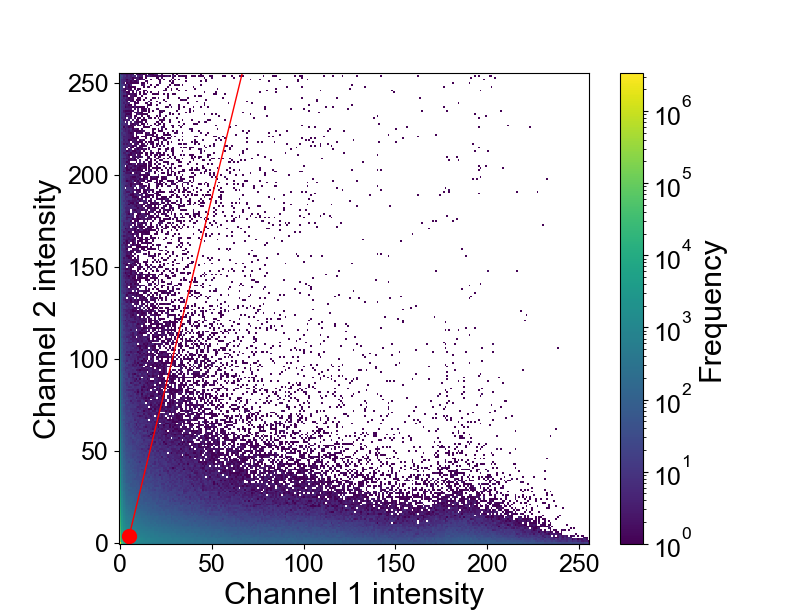
\includegraphics[width=0.49\linewidth]{figs/Placeholder_Image.png}}
    \subcaptionbox{3D intensity projection of all pixels above low threshold B\label{subfig:low_thresh_B}}{\includegraphics[width=0.49\linewidth]{figs/Placeholder_Image.png}}
    \caption[The outcome of the selected low threshold on area and separation of independent regions]{The outcome of the selected low threshold on area and separation of independent regions. The raw image is shown in Figure \ref{subfig:raw_3D} while both of the figures here (\subref{subfig:low_thresh_A}) and (\subref{subfig:low_thresh_B}) have different low thresholds of values A and B applied respectively where B is a low threshold value than A. \subref{subfig:low_thresh_A}) has smaller areas for the regions and which are also more separated, while in \subref{subfig:low_thresh_B}) the areas are larger yet previously separated regions are joined as shown in the annotated area of interest.}
    \label{fig:my_label}
\end{figure}
\fi
\subsubsection{Using Kneedle for low threshold approximation}\label{sec:low_thresh_kneedle}
%First, mention how Kneedle (ref the section) can be used to determine some turning point after a steep drop. Secondly, mention how this parts with our postulations where we will have some inital peak related to the background mode centred around the lowest background value (the size of the peak may vary but it is almost always there). Thirdly, mention how the log elbow was determined as a point to help with scenarios where it was fear to be too low. Lastly, mention the current selection criteria involving Otsu and the pros vs cons of it. There will be a single figure which will have the metric closeness and the voxel count closeness between Elbow, Log Elbow, Otsu, and Triangle.
The ``Kneedle'' algorithm (Section \ref{sec:kneedle}) is applied to the image histogram with the goal of approximating a sufficiently low threshold such that at least all of the `empty' background is captured within its range. This relies on the fact that Kneedle can determine either the knees or elbows within a function which can be characterised as the point of most sudden change in the gradient of the function after either increasing or decreasing respectively. For this application, the `empty' background is assumed to always be described by some crest among the lowest intensity values and it is the fall from this crest that is of interest. It was only after the application of this method and the evaluation of the binarized regions, regarding what it was certain was background from what might be foreground, that the effectiveness was observed. While the method at times fell short of the Expert values it frequently excluded the `empty' background values at least and was found to generally perform well. This can be seen in Figure \ref{fig:elbow_expert_compare} which compares the performance of the Kneedle low threshold, as well as Otsu and Triangle for reference as the prior best performers, to the Experts. While this comparison is reductive as it does not evaluate what is being binarized in the image (objects, shapes or patterns typically are passed through for evaluation by the High threshold) since it is a linear threshold it is known that if two thresholds are identical then their impact on the image binarization will be identical. From the results, it is seen that the results acquired by Kneedle are closer to the Experts across the span of samples and that the variance in the performance is tighter describing a more reliable outcome which is easier to predict. What may be noticed is that there is also a mention of ``Log Kneedle'' in both figures as well as ``Chosen Kneedle''.\paragraph{Log Kneedle} is the low threshold elbow that is acquired using the log of the histogram as opposed to the normal histogram. This application was hypothesised based on the notion that taking the log of the histogram will normalize and rescale it allowing the higher-intensity histogram components to be discerned if they have been drowned out by a huge `empty' background peak which can result in low threshold values that are too low. This is applicable as this log normalization allows large changes in the `empty' background, irregular background, and potential foreground intensity range to be evaluated in the histogram typically resulting in a higher elbow for the low threshold. Looking at Figure \ref{subfig:thresh_elbow} and \ref{subfig:voxel_elbow} it can be seen that the results of the Log Kneedle are highly varied in performance, particularly so for Expert A which also performed the worst, but its perspective on irregular background presence that the `empty' background might overshadow was believed to hold merit but not in the current approach.\paragraph{The Chosen Kneedle} was the approach which was established to tune whether to get the normal or log-transformed low threshold under some criteria. The criteria that were chosen were that if the Otsu threshold exceeded that of the Kneedle elbow then the log Kneedle elbow would be used instead. This was under the assumption that Otsu will be a poor performer given that the image quality resulted in the foreground and background modes being difficult to separate. The primary motivation behind this was that there were times when both the normal Kneedle elbow value and the Otsu value were too low leading to a greater amount of `empty' background being retained and diminishing the robustness of the high threshold approximation. This was a stopgap solution though and it cannot be reduced that the log Kneedle elbow value will be necessarily closer to the Experts but rather there is a significantly lower risk of `empty' background retention and the value still remains constrained.\textcolor{red}{I am slightly uncertain how to end this section. I feel that there is a distinct difference in the impact of both the Chosen and Normal Kneedle value although based on the similarity with the experts Normal appears to perform better but for cases where there is too much noise the normal incorrectly retains the chosen Kneedle is better. I could place a reference to Chapter 4 where the impact of each on the overall performance is evaluated?}
\iffalse
The 'Kneedle' algorithm (Section \ref{sec:kneedle}) is able to approximate turning points in distributions that are either \textit{knees} or \textit{elbows} where the elbow after the aforementioned low-intensity peak in the image histograms might be a sufficiently low threshold estimate. While this might not be the optimal low threshold in all samples particularly where the noise present persists into higher intensity ranges a slightly higher low threshold might be preferred but after manual evaluation over the 25 samples mentioned prior it was determined that in most cases it performed reasonably. This is supported by the results depicted in Figure \ref{fig:elbow_expert_compare} where in Fig. \ref{subfig:thresh_elbow} `Elbow Normal' can be seen to have a complete quartile range tighter than Otsu yet similar to Triangle meaning there is less variance in the difference from the experts than exhibited in Otsu. By observing the median line, where 50\% of sample values are situated above and below said line across the quartiles, it can be seen that in `Elbow Normal' the difference results typically skew in the direction of the zero line such that if the median is below zero then there is a positive skew meaning a greater proportion of those two quartile range values are closely situated around zero. In Fig. \ref{subfig:voxel_elbow} it can be seen that the `Elbow Normal' quartile distribution remains far tighter than that of Otsu and, surprisingly, Triangle although the median line positioning means that the skew tends towards zero strongly for only Expert A and C while only an outer quartile situates to zero for Expert B and D. Comparitively, Otsu only has noticeable skew with Experts B and C where the Median line lies on zero thus 
\fi
\begin{figure}
    \centering
    \subcaptionbox{Difference in threshold metric to be applied as the Hysteresis low threshold\label{subfig:thresh_elbow}}{\includegraphics[width=0.49\textwidth]{figs/ch3figs/Knee_Thresh_diff.png}}
    \subcaptionbox{Difference in voxel count post-binarization using the threshold value as the image would appear after low threshold application\label{subfig:voxel_elbow}}{\includegraphics[width=0.49\textwidth]{figs/ch3figs/Knee_Vox_diff.png}}
    \caption[Comparison between the thresholding method and the Experts for Otsu, Triangle, normal Elbow, log Elbow, and the chosen Elbow]{Comparison between the thresholding method and the Experts for Otsu, Triangle, normal Elbow, log Elbow, and the chosen Elbow. This comparison is depicted using box plots to describe the variance in the difference between the experts across multiple samples and the simplified distribution of these values.}
    \label{fig:elbow_expert_compare}
\end{figure}
\iffalse
The application of Kneedle to determine a low threshold was based on the hypothesis that selecting a low threshold around the elbow of the histogram would be able to remove the majority of the low intensity in the image. It was found though that at certain times the determined elbow would be sufficient for threshold use while at other times the determined elbow was too low of a value. For reference a human selected low threshold for each sample was chosen that was used to compare the ideal estimated low threshold compared to what was determined. In a fair number of samples it was found that the determined elbow was too low of a value (significantly lower than the expert selected low threshold) and an approach was required to determine a closer value while not fixating on the expert's exact value as it recognised that the value would be determined subjectively by the expert. Simultaneously it was speculated that although the exact value selected by an expert was subjective there would be underlying components informing that decision and perhaps these objective components could be inferred from the histogram. To better visualise the complete histogram and evaluate where structural information is present within the intensity range the logarithm of the histogram was implement in the elbow approximation. After some brief observations of a small subset of samples a second hypothesis was formulated that calculating the elbow of the log of the histogram could determine an elbow higher in value than before but not out of realistic range for a sample compared to the expert. After some tests this hypothesis was partially fulfilled particularly where the elbow of the normal histogram was found to be far lower than the desired low threshold.% Stipulate that the log was an earlier exploration of the histogram from a suggestion made during a disucssion with Rensu Theart
\par The final problem lay in selecting which elbow to use of either the normal histogram elbow or the log histogram elbow without prior knowledge of which elbow would be more desirable for a given sample. Tests with the Otsu threshold were performed to compare with the respective Kneedle results (normal and log) to investigate if the values could act as some form of decision criteria between the two elbow options. These tests were performed and the comparison between the elbow results produced by the Kneedle algorithm \cite{kneedle_arvai}; the Otsu, Mean, Yen and Triangle thresholds in scikit-image \cite{scikit-image}; and the threshold values manually determined by an expert. Using this comparison it was observed that when the Otsu threshold was greater than the normal histogram elbow that the log histogram elbow was a closer threshold value to that selected by the expert while an Otsu value less than or equal to the normal histogram elbow occurred when the normal histogram elbow was closer to the threshold value selected by the expert. To evaluate the performance of this a test was performed involving a reference threshold which was generated for each image using expert low and high thresholds which was compared to images of the same corresponding samples but the low threshold was determined using one of the aforementioned automated methods. The automated threshold images used an automated low threshold determined by the Triangle, Otsu or best fit elbow method while the high threshold used for the image was still the expert high threshold such that only the relative impact of the low threshold was evaluated. The measure used to compare these partially automated threshold images and the expert reference image is the structural image overlap similarity measure described in Section \ref{sec:similarity_metric}. From Fig. \ref{subfig:low_boxplot} it can be seen that while the Otsu and Knee results share the same median value the interquartile range of the Knee results are not as wide as that of the Otsu results thus there is greater consistency in the performance of the Knee results across the tested samples. While the Triangle results have the narrowest interquartile range it is observed that the median similarity metric is the lowest and the upper quartile is lower than both the Otsu and Knee upper quartiles. In Fig. \ref{subfig:low_mean} the height of the bars depict the average similarity measure for each threshold measure across the test sample range. Of these average similarity results it is seen that the Knee threshold achieve a greater average similarity than the other threshold methods. Further analysis of these results is discussed in Section \ref{sec:low_thresh_metrics} but what can be summarised is that the selective Kneedle algorithm produces threshold images that achieve the highest similarity on average, have the highest minimum similarity across the sample set and provide the second most consistent results based on the interquartile range. %Need to also do a comparison comparing chosen vs normal vs log to determine why it is best to select the knee approach
\begin{figure}[h!]
    \centering
    \subcaptionbox{Sample histogram of the complete intensity range\label{subfig:noisy_hist}}{\includegraphics[width=0.48\linewidth]{figs/hist.png}}
    \subcaptionbox{Sample histogram with an intensity range from the low intensity elbow to the maximum}{\includegraphics[width=0.48\linewidth]{figs/hist_cut.png}}
    \subcaptionbox{The log representation of the sample histogram for the full intensity range}{\includegraphics[width=0.48\linewidth]{figs/hist_log.png}}
    \subcaptionbox{The log representation of the sample histogram for the intensity range from the original histogram low intensity elbow}{\includegraphics[width=0.48\linewidth]{figs/hist_log_cut.png}}
    \caption{Sample histograms of the intensity frequency across the intensity range. A black vertical line designates the estimated elbow of the histogram}
    \label{fig:sample_hist_for_low}
\end{figure}
\fi
\newpage
\subsection{High threshold acquistion}
With the low threshold for a given sample image selected the final step is to approximate a suitable high threshold value. While the low threshold approximation was also challenging the high threshold was a more complex problem due to the image histogram being comparatively less useful. While images with clearly depicted foreground and background modes in the histogram allow for the high threshold to be selected, relative to the foreground mode, this is not the case in images where the foreground mode is unclear. This is typically due to either out-of-focus fluorescence, higher-intensity noise components not removed by denoising, unexpectedly stained biomolecules (e.g. free-floating proteins in the Cytoplasm), or image artefacts. The former two are addressed by deconvolution and denoising respectively during pre-processing although when the presence is too strong there may be interferences remaining, particularly with noise as overly aggressive denoising can degrade the image signal, yet the latter two cannot be addressed as easily with most methods although appropriate image thresholding is one of the means to address this. The reason for this is that many thresholding methods can be tuned to preserve the actual foreground objects in the image while both rejecting the remainder as background and minimizing image signal degradation. The images worked with in this research exhibit all four of the aforementioned obstructions, in different severities, to effectively separate the foreground and background modes thus a means of estimating an optimal labelling of foreground objects. \paragraph{Design considerations made for foreground acquisition} were important to make as this method could not rely on some known perfect output but rather had to find some result which provided the best-estimated outcome. There were three primary considerations that were made which are:
\begin{enumerate}
    \item The system must adapt to each image to get an image-specific outcome but apply identical logic to all of them
    \item Image attributes used in the system must relate to the intensities of the potential foreground voxels
    \item If the system makes an error then it must be done in a manner that is the least detrimental to future analysis
\end{enumerate}
To address these considerations intensity-related attributes such as the pixel/voxel intensity distribution visualised by the histogram and intensity distributions across pixel neighbourhoods were raised. The primary problem with these is that utilizing the voxel intensity distribution across the image encounters the same problems of mode separation which confronts global threshold methods while neighbourhood-based approaches where the intensity distribution is aggregated encounter the parameter selection obstacles of local threshold methods where the size of the neighbourhood, among other parameters, directly affects performance. Since the low threshold had already been resolved a method that evaluates only the impact of the high threshold was required and led to a hypothesis that if the impact of the high threshold on the image across a threshold range could create a distribution then perhaps that could describe other image features?

\subsection{Iterative hysteresis histogram (IHH)}\label{sec:ihh}
%Define an acronym for this IHH and how this is constructed by iterating the high threshold until it equals the low thresh for hysteresis and the number of retained voxels is counted.
This method was termed iterative hysteresis histogram (IHH), which is a distribution relating to the high threshold hysteresis application but also the name of the method by which it is acquired. This distribution is the total count of potential foreground voxels at each high threshold where the high threshold ranges from 1 intensity above the low threshold up to the maximum image intensity. An example illustrating the approach used to construct the IHH is shown in Figure \ref{fig:ihh_sequence} where a microscope maximum intensity projection (MIP) image is used for illustrative purposes. This culminates in a distribution that begins at \underline{one above} the low threshold intensity with some maximum count $X$ which is a non-increasing function $f(x)$ which can either remain the same or decrease as $x$ increases (where $x$ is the high threshold value). Due to this non-increasing nature of the function, the largest magnitude of $f(x)$ will be at the lowest possible $x$ value (one above the low threshold) and the shape of $f(x)$ across the intensity range can describe certain image properties. This distribution across the high threshold range can describe the foreground `confidence' of structures within the image as higher intensities are more likely to compose the foreground as the intensity tends towards the maximum intensity (similar to the background confidence baseline described at the end of Section \ref{sec:low_acquis}). The reason for this confidence is that voxel intensities within the image are chiefly dependent on how in-focus the emitting fluorophores are implying that it is highly likely that the depth at which the captured fluorescence originates aligns with the depth described in the image and that there is a reasonably high density of fluorophores at that position such that the increased density of fluorescence originating from said point result in a higher combined intensity value in the image. This assumption functions as a heuristically based justification for this confidence but is not the sole reason and only functions under the assumption that the quality at which the image is captured is sufficient such that foreground and background separation can be performed using visual analysis performed by a human. As illustrated in Figure \ref{fig:ihh_contrast_compare} an image with a well-separated foreground and background has a more rectangular IHH (Fig. \ref{subfig:mip_good_contrast_ihh}. \& \subref{subfig:rectangular_ihh}. for MIP and IHH respectively) where the high peak in count in the highest intensities depicts that a large proportion of the structures persist from a strict high threshold and only a few additional structures appear at the lower intensities. The opposite is seen in the poorly separated foreground and background (Fig. \ref{subfig:mip_bad_contrast_ihh}. \& \subref{subfig:sloping_ihh}. for MIP and IHH respectively) where the sloping nature of the IHH reflects the dispersion of the structures across the range of intensity values increasing the difficulty in evaluating what is and is not of the foreground in the image. The challenge is that there are few algorithmic ways in which to quantify the shape of the IHH and consistent logic by which to evaluate it compared to some metric such as standard deviation or variance for example.  

\begin{figure}
%This will be a sequence of images to show how the IHH is determined. 1. The raw MIP; 2. The MIP with bordering around the structures; 3. The structures colour coded to show the independent volumes; 4. The colouring changed to match the brightest pixel in the structure and a legend denoting that; 5. The IHH with vertical lines annotating where certain structures appear at. If borders cannot be placed then ignore 2.
    \centering
    \subcaptionbox{Raw MIP of a microscopy image\label{subfig:raw_mip_sequence}}{\includegraphics[width=0.32\textwidth]{figs/ch3figs/Before_Hyst.png}}
    \subcaptionbox{Structures labelled using unique colours for differentiation\label{subfig:colour_coded_sequence}}{\includegraphics[width=0.32\textwidth]{figs/ch3figs/Mid_Hyst.png}}
    \subcaptionbox{Structures coloured based on brightest contained pixel intensity\label{subfig:pixel_intensity_sequence}}{\includegraphics[width=0.32\textwidth]{figs/ch3figs/Intensity_labels.png}}
    \subcaptionbox{IHH of image with annotations regarding the highest intensity possessed by each structure\label{subfig:annotated_ihh_sequence}}{\includegraphics[width=\textwidth]{figs/sample_ihh.png}}
    \caption[An illustration of the sequence by which the IHH is determined for a cell image]{\textcolor{red}{The IHH in Figure \ref{subfig:annotated_ihh_sequence} is supposed to have colour coding that matches the structure colours in \ref{subfig:pixel_intensity_sequence}}An illustration of the sequence by which the IHH is determined for a microscopy cell image. The image used is a 2D maximum intensity projection of an original 3D image for illustrative purposes. This depicts how \textbf{\subref{subfig:raw_mip_sequence})} the raw image appears initially; \textbf{\subref{subfig:colour_coded_sequence})} the labelling of the independent structures in the image which are labelled by both colour and a numeric annotation; \textbf{\subref{subfig:pixel_intensity_sequence})} the structures are now re-coloured based on the highest pixel intensity contained within it which is also reflected in the annotated labels; \textbf{\subref{subfig:annotated_ihh_sequence})} lastly, the IHH that is constructed from the sum of the volumes of each structure from the lowest intensity up until their respective maximum.}
    \label{fig:ihh_sequence}
\end{figure}
\begin{figure}
    \centering
    \subcaptionbox{MIP of well separated foreground and background \label{subfig:mip_good_contrast_ihh}}{\includegraphics[width=0.49\textwidth]{figs/ch2figs/CCCP_1C=1T=0_normal.png}}
    \subcaptionbox{IHH of \subref{subfig:mip_good_contrast_ihh}) \label{subfig:rectangular_ihh}}{\includegraphics[width=0.49\textwidth]{figs/sample_ihh.png}}
    
    \subcaptionbox{MIP of poorly separated foreground and background \label{subfig:mip_bad_contrast_ihh}}{\includegraphics[width=0.49\textwidth]{figs/ch2figs/CCCP_1C=1T=0_normal.png}}
    \subcaptionbox{IHH of \subref{subfig:mip_bad_contrast_ihh}) \label{subfig:sloping_ihh}}{\includegraphics[width=0.49\textwidth]{figs/sample_ihh.png}}
    \caption[Examples of two opposing IHH's from images with good and bad foreground to background separability.]{Examples of two opposing IHH's from images with good and bad foreground to background separability.}
    \label{fig:ihh_contrast_compare}
\end{figure}

\subsubsection{Using the IHH}
While it was realized that the IHH captured information regarding the foreground and background separation of an image in a non-increasing distribution the challenge remained in reliably exposing features to quantify without muddling the understanding of what the distribution describes. After evaluating the IHH shape and its implications regarding the distribution of potential foreground over a range of high threshold strictness it was hypothesized that desired thresholds are likely to situate around ``flat'' regions of the IHH. The reason that ``flat'' IHH regions were of interest is based on what the IHH itself describes which is the distribution of the maximal intensity of each structure in the image (after low threshold application) with structures persisting at larger high thresholds being more within focus in the image. These flat regions were typically selected at lower high threshold intensities since we want to include as many potentially viable foreground structures in future analysis but this was based on an observation made with visual analysis. Regardless, this lead to the investigation of two fronts:
\begin{enumerate}
    \item Is a desirable threshold typically located on or adjacent to a relatively ``flat'' region of the IHH?
    \item How can this be quantified in a manner which can be fed into an algorithm?
\end{enumerate}
\textcolor{red}{Do you think I should include a few examples showing that the relatively flat regions of the IHH correlate with being near a threshold that would render a viable binarization outcome?}
With the objectives made clear experimentation began where the first objective was heuristically confirmed, although partially, that although there was no definitive proof there was a near pattern where `viable' high thresholds were situated near relatively flat IHH regions with a low margin of error. The real challenge came into the quantification of this with regard to detecting a `flat' region (how flat must it be for consideration?) and if there are multiple flat regions how should the selection be made between them?
\subsubsection{IHH gradient} 
The IHH gradient was believed to be the most effective solution to this where a gradient instead of a derivative would be used. The reason that either of these would be used is that if the slope of the IHH can be seen as representing the change in the IHH value then a flat IHH region would have no slope where the steepness of the slope is described by the gradient or the derivative. The gradient is what was decided to be used as the derivative requires some generalization of the IHH distribution function but said function cannot be inferred from the IHH thus the gradient evaluated against the distribution itself is more viable where the change in the IHH magnitudes ($y(n)$) between sequentially increasing intensity values ($x(n)$) can be measured as shown in Equation \ref{eq:slope_eq}. An illustration of an IHH and the gradient representation ($y'(n)$) can be seen in Figure \ref{fig:ihh_grad_compare}.
\begin{equation}\label{eq:slope_eq}
    m(n) = \lvert\frac{\Delta y(n)}{\Delta x(n)}\rvert = \lvert\frac{y(n)-y(n-1)}{x(n)-x(n-1)}\rvert\text{ where $N\geq n\geq 1$}
\end{equation}
\textcolor{red}{I am also considering having a figure where I highlight a region of the gradient representation with a high magnitude and match it to the same intensity window in the normal IHH and then colour code an MIP accordingly. The colouration in both graphs will be based on the intensity (the high threshold value that the pop out after) and this colouring will be mapped to the MIP with all other structures remaining grayscale. This would illustrate how an intensity range in flux could be composed of uncertainty. The same could be done with flat regions. Let me know your thoughts.}
\begin{figure}
    \centering
    \subcaptionbox{The original image IHH\label{subfig:original_ihh}}{\includegraphics[width=0.48\textwidth]{figs/sample_ihh_bad.png}}
    \subcaptionbox{The gradient representation of \subref{subfig:original_ihh})\label{subfig:discrete_grad}}{\includegraphics[width=0.48\textwidth]{figs/norm_ihh_slopes.png}}
    \caption[Comparison between the original IHH representation and the IHH gradient of Figure \ref{subfig:mip_bad_contrast_ihh}]{Comparison between the original IHH \textbf{(\subref{subfig:original_ihh})} representation and the IHH gradient \textbf{(\subref{subfig:discrete_grad})} of Figure \ref{subfig:mip_bad_contrast_ihh}}
    \label{fig:ihh_grad_compare}
\end{figure}
\paragraph{The problem} is that the gradient that we calculated does express the change in total structure volumes at increasing high threshold strictness but it is quite discrete as it only measures this change between consecutive intensities and it cannot capture changes expressed across an extended range of intensities and it is not uncommon for trends to be expressed over a range of values based on the shape of the IHH. A second problem found from this is that the resulting gradient distribution can have a noisy appearance due to the discrete approach used to calculate the gradient representation, as can be seen in Figure \ref{subfig:discrete_grad},  which increases the difficulty in numerically evaluating trends in the distribution to estimate where might be a potential point for high threshold selection. An example of this would be if, hypothetically, the ideal point is the minimum value within the distribution or some minima going from the lowest point of the high threshold range to the maximum. It could be caught in a sub-optimal local minima. These examples are stated while ignoring the potential challenges or problems those methods raise but regardless this noisy representation obscures the trends in the gradient representation that actually describe the high threshold strictness (or sensitivity) behaviour for an image and how the overall binarization responds to said behaviour.
\paragraph{The solution} proposed was to apply a smoothing operation using a rolling average where an intensity window (of size $W$) is designated and centred on a gradient representation magnitude $y'(n)$ at an intensity $n$. This centred window is then rolled across the full range of intensities $N$ where the average $\overline{y}'(n)$ is used as the new smoothed gradient value ($\overline{y}'(n)$ at $n$. This is seen in Equation \ref{eq:average_window} with $m_1$ and $m_2$ being the bounded upper and lower window ranges as described in Equation \ref{eq:av_win_conditions} where $m_1$ and $m_2$ are both $W/2$ save for when the centre of the window ($n$) is too close to the bottom ($n\to 0$) or end ($n\to N$) of the range. When the centre is too close the lower ($m_1$) or upper ($m_2$) bound of the window is shortened to fit in the reduced range and so too is the length of the window by which the value is divided by, given that the window contains less values to average.
\begin{align}\label{eq:average_window}
        \overline{y}'(n) &= \frac{\sum_{t=n-m_1}^{n+m_2}y'(t)}{m_1+m_2}\\ \label{eq:av_win_conditions}
    \text{ where }m_1 &=\begin{cases}
        0, & \text{if } n=0\\
        \leq W/2, & \text{if } n \leq W/2\\
        w/2, & \text{if } n \geq W/2
    \end{cases}
    \text{and }m_2 = \begin{cases}
                0, & \text{if } n=N\\
        \leq W/2, & \text{if } n \geq N-W/2\\
        w/2, & \text{if } n \leq N-W/2
    \end{cases}
\end{align}
\textcolor{red}{Here I state that the window size will be 8 for use in the system development. Should I in Chapter 4 briefly explore the impact of the window size on the system results or should I append that to this subsection or chapter?}
Through heuristic testing, a window size of $8$ was decided for use as it did not overly smooth the distribution via diminishing the trends but noisy behaviours were sufficiently suppressed. This was evaluated by visual analysis of the smoothed gradient representation of the IHH were it was observed that a smoothing window of $8$ functioned optimally for a subset of samples but further testing will be performed accompanied by numerical evaluations of the impact on performance the window size has. 

\subsubsection{IHH gradient inversion}
With the discrete noisy behaviour smoothed down while preserving the trends, a method to identify ideal regions was still required although the basis that flat IHH regions will inform this was still maintained. As comparatively flatter regions of the gradient IHH contribute more weight to the high threshold selection an inversion of the gradient representation magnitude is performed such that the values used in the distribution better reflect the intended use of them in further algorithms. There were two methods by which the representation was to be inverted with the first being a sigmoid-based approach while the latter was a linear inversion. This sigmoid-based approach would employ the use of the logistic function to invert the smoothed gradient distribution to invert and scale the weight contributions of flatter regions. The motivations around this were initially that the occurrence of completely ``flat'' regions in the gradient distribution was ideal but also naive and there was no certainty that it would be present within any of the distributions. Due to this flatness limitation, a softer inversion method using the logistic function that could be tuned was first approached. This application projected the gradient representation magnitudes ($y$-axis) along the logistic function dependent variable ($x$-axis) with the resulting new magnitudes being based on the steepness parameter of the logistic function. What is consistent is that the lowest gradient magnitude will become $1$ after re-weighting while the maximum gradient magnitude will become $0$ but a steepness parameter with a resulting \textit{S}-shaped curve, as shown in Figure \ref{fig:logistic_rescaling}, will result in a clustering of $n$ of the bottom and top of the gradient magnitude. This results in a new distribution that essentially states ``values close to the peak are essentially all experiencing too much change while values within a low enough margin of magnitude of change are approximately the same'' reducing nuance but also emphasizing broad trends of the extreme gradient representation values. 
\begin{figure}
    \centering
    \subcaptionbox{Logistic inversion function with low steepness \label{subfig:low_steep_logist}}{\includegraphics[width=0.49\textwidth]{figs/Rescale_dist_6.png}}
    \hfill
    \subcaptionbox{Logistic inversion function with high steepness\label{subfig:high_steep_logist}}{\includegraphics[width=0.49\textwidth]{figs/Rescale_dist_50.png}}
    \subcaptionbox{Resultant Inversion using a low steepness logistic function\label{subfig:low_steep_invert}}{\includegraphics[width=0.49\textwidth]{figs/Logist_rescale_slope.png}}
    \hfill
    \subcaptionbox{Resultant Inversion using a high steepness logistic function \label{subfig:high_steep_invert}}{\includegraphics[width=0.49\textwidth]{figs/Logist_rescale_slope_50.png}}
    \subcaptionbox{Original smoothed Gradient IHH with the projected logistic function (low steepness) parallel to the $y$-axis and the resulting inversion parallel to the $x$-axis \label{subfig:low_steep_joint}}{\includegraphics[width=0.49\textwidth]{figs/Joint_rescale_ihh.png}}
    \hfill
    \subcaptionbox{Original smoothed Gradient IHH with the projected logistic function (high steepness) parallel to the $y$-axis and the resulting inversion parallel to the $x$-axis \label{subfig:high_steep_joint}}{\includegraphics[width=0.49\textwidth]{figs/Joint_rescale_ihh_50.png}}
    \caption[Logistic function projection of smoothed gradient representation magnitudes with resulting re-weighting]{Logistic function projection of smoothed gradient representation magnitudes with resulting re-weighting. The original IHH can be seen in Figure \ref{subfig:discrete_grad} with the logistic function to invert it shown in figures (\subref{subfig:low_steep_logist}) and (\subref{subfig:high_steep_logist}). The resultant inversion is shown in figures (\subref{subfig:low_steep_invert}) and (\subref{subfig:high_steep_invert}). A final representation is shown in Figures (\subref{subfig:low_steep_joint}) and (\subref{subfig:high_steep_joint})
    }
    \label{fig:logistic_rescaling}
\end{figure}
This introduced a new tunable parameter and although a value of $6$ was settled on, for the purposes of developing subsequent features, further rigorous testing would be required to fully discern the impact of the logistic function shape, based on the steepness parameter, on the behaviour of the high threshold determination. Due to this, a more clear linear inversion was introduced in Equation \ref{eq:linear_inv} where the magnitudes of the smoothed gradient distribution ($\overline{y}'(n)$) are subtracted from and divided by the maximum of the distribution ($\overline{Y}'_{\text{maximum}}$) for all intensity values ($n$) resulting in a normalized and flipped smoothed gradient distribution ( $\overline{y}'_{\text{new}}(n)$ ). The benefit of this is that the inversion will perform relatively consistently for gradient distributions regardless of the source image and that there will be no added tunable parameters while still achieving the desired outcome of emphasizing lower values in smoothed gradient distribution numerically.
\begin{equation}\label{eq:linear_inv}
    \overline{y}'_{\text{new}}(n) = \frac{\overline{Y}'_{\text{maximum}} - \overline{y}'(n)}{\overline{Y}'_{\text{maximum}}}
\end{equation}

\subsection{Selecting a high threshold}\label{sec:centroid_calc}
With the smoothed gradient IHH distribution inverted such that values of lower change in IHH values are emphasized a high threshold value needs to be selected. The key challenge regarding high threshold selection using the gradient distribution is the criteria used to determine what region is best fit as there can be multiple regions of varied degrees of flatness in the IHH which are expressed in the gradient representation with the result needing to be a single value. There were many attempts to determine a value similar to a mean of the intensities based on the inverted gradient distribution as weights and after experimentation, a method to achieve this was produced as shown in Equation \ref{eq:first_centroid}. In this function, there are $N$ sequential intensity values $x(n)$ that make up the $x$-axis of the inverted gradient distribution with the inverted gradient values $\overline{y}'_{\text{new}}(n)$ is used to weight the intensity value for each corresponding intensity $n$ and averaged by the total count of values composing the distribution $x$-axis. 
\begin{equation}\label{eq:first_centroid}
    C = \frac{\sum_{0}^{N} \overline{y}'_{\text{new}}(n)\circ x(n)}{N}
\end{equation}
The result of this is a value that acts similar to a centre of mass ($C$) for an object given that the inverted gradient magnitudes represent the mass contributions of each intensity value in the distribution thus some `best fit' result is achieved that takes all values across the distribution into account. After it was confirmed that this resulted in an intensity value calculated based on the gradient magnitudes the spectral centroid was discovered. Due to the greater context of how the algorithm should behave, based on Eq. \ref{eq:first_centroid}, the centroid calculation was discovered where a crucial difference is that the value is divided by the sum of the inverted gradient weights across the intensity range ($\sum_{0}^{N}\overline{y}'_{\text{new}}(n)$) as seen in Equation \ref{eq:actual_centroid}. The added benefit of this approach is that the divisor is the sum of intensity weights ($\sum_{0}^{N}\overline{y}'_{\text{new}}(n)$) resulting in a more accurate intensity centroid ($C_x$) using a method that is more mathematically robust which is more applicable to this use case.
\begin{equation}\label{eq:actual_centroid}
    C_x = \frac{\sum_{0}^{N} \overline{y}'_{\text{new}}\circ x(n)}{\sum_{0}^{N}\overline{y}'_{\text{new}}(n)}
\end{equation}
This final intensity centroid considers the distribution of `flatness' throughout the IHH which is expressed as values tending towards $1$ in the inverted gradient representation magnitude and selects a best-fit value but it was found that at times that the higher contrast resulted in very flat high intensities that contained far less object information than desired and the general approach is that if the system outcome is going to err then rather it err more lenient and preserve more voxels as foreground as these can be addressed with further processing but any voxels labelled as background may be wholly excluded from any further processing or evaluation risking information being lost.
\begin{figure}
    \centering
    \subcaptionbox{Distribution showing the inverted gradient representation with the two centroid outcomes annotated by vertical, dashed lines}{\includegraphics[width=0.59\textwidth]{figs/ch3figs/centroid_correction.png}}
    \subcaptionbox{The effect of these outcomes on the image thresholding. Blue describes the voxels above the low threshold; green describes all structures containing a voxel intensity above the incorrect centroid (\ref{eq:first_centroid}); and red describes all structures containing a voxel intensity above the correct centroid (\ref{eq:actual_centroid})}{\includegraphics[width=0.39\textwidth]{figs/ch3figs/centroid_compare.png}}
    \label{fig:centroid_illustration}
    \caption[A comparison between the initial centroid method(incorrect centroid) and the robust method that is used (correct centroid)]{A comparison between the initial centroid method(incorrect centroid) and the robust method that is used (correct centroid). The difference in the centroid value outcome is illustrated on an inverted gradient distribution line plot where dashed vertical lines are used to illustrate the centroids while the difference in the impact on the Hysteresis thresholding results are displayed using a MIP image. The image is colour-coded to differentiate and aid in comparison between the threshold outcomes}
\end{figure}
%look up if there is any benefit due to the divider that is documented
%Mention that it is the more robust approach
%This is all we really have. Show two tot three diagrams for how this selects values and move one (we can't say why better so we test it [between the two centroid approaches])
\subsection{Applying biases to the centroid result}\label{sec:system_biases}
As it was found that at times the centroid result returned a high threshold that was too strict biases were developed to balance this. The reason for this is speculated to be due to the reduction in the context of the objects depicted in the image due to the quantification of image properties. Primarily is this IHH distribution which describes the response behaviour of the image to varied high threshold strictness but does not provide the nuance to know when it is relegating a large number of image structures to the background as opposed to the foreground nor can it consider properties such as the shape or volume of the individual potential foreground structures in an effective manner. To address this two biases were applied.

\subsubsection{IHH total volume bias}
So as to add some bias to the high threshold determined using the centroid a second weighting metric was added which was based on the normalized IHH distribution for the image. This is applied to the numerator and denominator within the summation as shown in Equation \ref{eq:vox_weight_added}. By doing so we introduce the context of the distribution of foreground information which the IHH describes as the $y$-axis representing the number of foreground voxels for each $x$-axis value representing the high threshold (therefore the strictness of the high threshold) resulting in an IHH weighting $v(n)$.
\begin{equation}\label{eq:vox_weight_added}
    C_x = \frac{\sum_{0}^{N-1} v(n)\circ \overline{y}'_{\text{new}}(n)\circ x(n)}{\sum_{0}^{N}\overline{y}'_{\text{new}}(n)\circ v(n)}
\end{equation}
The effect of this can be seen in Figure \ref{fig:distro_centroid_compare} where the difference between the centroid determined using the inverted gradient representation of the IHH can be greatly skewed by the application of the normalized IHH distribution. In this figure, the distributions (separated and combined) for two sample images deviate further from the separate centroids the faster the IHH distribution decays relative to the increasing high threshold intensity along the x-axis. This means that although the centroid of two IHH distributions can be close between two samples their influence on an identical inverted gradient distribution is less predictable. The benefit of this is that the strength of this bias is dependent on the distribution of the potential foreground structure information across the high threshold intensity span. Better separated foreground structures with a higher contrast will typically result in distinctly rectangular distributions or ones that decay in wider steps and are more robust to fluctuations in the high threshold value.\par
\begin{figure}
%This will be 4 graphs with two per sample. One graph type will have two overlayed lineplots (inverted and IHH with each having own centroid) and a second graph type for when the weighting is applied with the resulting new centroid. 
    \centering
    \subcaptionbox{Inverted and normalized IHH distributions for a sample A with dashed vertical lines for the centroids \label{subfig:separate_distrosA}}{\includegraphics[width=0.49\textwidth]{figs/ch3figs/distros_with_centroids_separateA.png}}
    \subcaptionbox{The inverted gradient distribution with the normalized IHH weighting applied and a dashed vertical line representing the centroid for a sample A \label{subfig:combined_distroA}}{\includegraphics[width=0.49\textwidth]{figs/ch3figs/both_distro_combinedA.png}}
    \subcaptionbox{Inverted and normalized IHH distributions for a sample B with dashed vertical lines for the centroids \label{subfig:separate_distrosB}}{\includegraphics[width=0.49\textwidth]{figs/ch3figs/distros_with_centroids_separateB.png}}
    \subcaptionbox{The inverted gradient distribution with the normalized IHH weighting applied and a dashed vertical line representing the centroid for a sample B \label{subfig:combined_distroB}}{\includegraphics[width=0.49\textwidth]{figs/ch3figs/both_distro_combinedB.png}}
    \caption[A showcase comparing the influences of the inverted gradient and normalized IHH distributions on the centroids separately and when combined]{A showcase comparing the influences of the inverted gradient and normalized IHH distributions on the centroids separately and when combined. In the figures illustrating both the separate distributions in red and green (Fig. \ref{subfig:separate_distrosA} \& \ref{subfig:separate_distrosB}) and the new distribution produced by multiplying said distributions and determining a new centroid (Fig. \ref{subfig:combined_distroA} \& \ref{subfig:combined_distroB}). By comparing the change in the determined centroids when the distributions are combined for Samples A (Fig. \ref{subfig:separate_distrosA} \& \ref{subfig:combined_distroA}) and B (Fig. \ref{subfig:separate_distrosB} \& \ref{subfig:combined_distroB}) it can be observed that the new centroid determined in the former sample is at a lower value than either of the separate centroids while for the latter sample the new centroid is far closer to the separate centroids of the original distributions. This highlights the impact the shape of the distribution has on the calculated centroid value.}
    \label{fig:distro_centroid_compare}
\end{figure}
The reason for this is the leniency towards false positives over false negatives for foreground selection as erroneously labelled foreground can be removed with further processing yet the background erroneously labelled background is typically lost to further analysis. Since the high threshold selection is expected to be a best-fit approximation, tending towards a precise value, it is supposed that there will be some level of error and despite a goal being to minimize this error it was decided that it would rather err to a lower high threshold value as opposed to a higher value. A fixed shift in the approximated towards the lower intensity values was deemed inapplicable as it is naive to the imaging conditions and uniqueness presented by each sample image and no single value would work, this shift would need to adapt to the image. This is the reason that the IHH was chosen since tending the high threshold range towards the lower end typically results in a plateau or increase in IHH magnitude implying an increase in potential foreground information. As we tend to a lower high threshold value the risk of the potential foreground voxels being that of noise increases relatively speaking thus this is used in conjunction with the inverted gradient representation of the IHH with the intention that each compensates for the other.
\begin{figure}
%This will contain the raw MIP of one sample from above. There will be a structure highlighting MIP as well. An RGB overlay of the normal centroid (R) and the centroid from just the IHH (G). Lastly, there will be a viridis MIP showing the new centroid effect combined with structure highlighting. This way the graphs don't have to be shown again and only MIP displayed
    \centering
    \subcaptionbox{Raw image with no thresholds applied\label{subfig:mip_centroid_compareA}}{\includegraphics[width=0.49\textwidth]{figs/ch3figs/raw_mip.png}}
    \subcaptionbox{The potential foreground structures are highlighted with different colours based on the maximum voxel intensity contained within after a low threshold has been applied\label{subfig:mip_centroid_compareB}}{\includegraphics[width=0.49\textwidth]{figs/ch3figs/highlight_mip.png}}
    \subcaptionbox{A red, green and blue (RGB) each colour channel labels regions above a specific threshold. The red, green, and blue channels represent the voxels of structures containing an intensity greater than that of the threshold derived using the inverted gradient distribution, the IHH distribution, and the product of both distributions respectively. The cyan regions are where green and blue overlap and the grayscale regions are where all three channels overlap.\label{subfig:mip_centroid_compareC}}{\includegraphics[width=0.49\textwidth]{figs/ch3figs/rg_mip.png}}
    \subcaptionbox{The structures are colour-coded according to the maximum structure intensity of each. The structures remaining are those that have a maximum intensity greater than the centroid of the inverted gradient distribution after the normalized IHH distribution has been applied as weighting\label{subfig:mip_centroid_compareD}}{\includegraphics[width=0.49\textwidth]{figs/ch3figs/weighted_mip.png}}
    \caption{The images shown are MIP images of a sample image where the differences of the different centroids, determined using the relevant distributions, are illustrated.\label{fig:centroid_weighting_mips} \textcolor{red}{I feel the caption of the RGB subfigure is a bit too long, do you have any suggestions? Perhaps I should summarize the subfigure captions and move the descriptions to the main caption?}}
\end{figure}
Figure \ref{fig:centroid_weighting_mips} illustrates the effect of these different centroid results on the hysteresis thresholding outcome. The distributions shown in Figure \ref{fig:distro_centroid_compare} (\subref{subfig:separate_distrosA}) and (\subref{subfig:combined_distroA}) are for this same sample image and in the red and green centroids shown in (\subref{subfig:separate_distrosA}) match to the red and green colour channels shown in Figure \ref{subfig:mip_centroid_compareC} (red and green overlap appears as yellow). Despite the green channel threshold (based on the IHH distribution centroid) being lower than that of the red channel the final centroid calculated from the IHH weighted inverted gradient distribution (Fig. \ref{subfig:combined_distroA}) contains more structures than even the green channel as the centroid value is of an even lower value. This will provide a bias which will provide a lower high threshold intensity than the inverted gradient distribution along with the magnitude of this bias being image dependent meaning that the bias adapts to the sample image as opposed to some fixed value that needs to be entered for each sample.

\subsubsection{Shrinking window bias}
A second kind of bias that was implemented was the sliding window bias which affects the distribution for which the spectral centroid is calculated. This base premise is that within the intensity range above the low threshold, the lowest intensity value is supposed to be to the left while the highest intensity is to the right where the window initially spans from the furthest left with the upper range of the window ($I$) iterating across the range $I=[x_{min}+1, X]$. This range begins at $x_{min}+1$ which is 1 value greater than the smallest value within the original range after the low threshold application thus the lowest intensity value is not necessarily $0$. This is described in Equation \ref{eq:window_centroid}, and illustrated in Figure \ref{fig:window_approach}, which shows how the centroid ($C_I$) would be calculated for a window with an intensity upper bound of $I$ where in this figure there are three windows shown, with the respective centroids, with varied window sizes to illustrate the effect on the centroid value a narrower distribution has. This can be applied in conjunction with the IHH total volume bias with $\overline{y}'_{\text{new}}$ substituted for $v_w(i)\circ \overline{y}'_{\text{new}}(i)$.
\begin{equation}\label{eq:window_centroid}
    C_I(d) = \frac{\sum_{i=x_{min}}^{d} \overline{y}'_{\text{new}}(i)\circ x(i)}{\sum_{i=x_{min}}^{d}\overline{y}'_{\text{new}}(i)} \text{ where } d \leq X \text{ and } d \subset X
\end{equation}
\begin{figure}
%This will be a figure where an annotation will be made for the hypothetical window frame using I for the window and (X-I) for the excluded part outside the window. The original centroid could be shown and the window centroid will be shown as well using dashed lines
    \centering
    \includegraphics[width=\textwidth]{figs/ch3figs/Windows_overlapping.png}
    \caption[An example of how the window weighting approaches are applied to the distributions]{An example of how the window weighting approaches are applied to the distributions where in this example there are three bounded windows shown. The spans of these windows are annotated below the x-axis using coloured, horizontal lines with an accompanied label where window 1 ($W_1$) is shown with red, window 2 ($W_2$) is shown with green, and window 3 ($W_3$) is shown with blue. Each of these windows also has a respective centroid calculated for the distribution that falls within the window range which is annotated by a dashed vertical line with the appropriate colouring to match the windows and a label $C_n$ where $n$ is for the respective window. There is a black dashed vertical line with the label $C$ which represents the distribution centroid for the whole distribution without the windows}
    \label{fig:window_approach}
\end{figure}
As mentioned, this function will be performed for each iteration of $I$ resulting in numerous windowed centroids $C_I(I)$ across the window width range which will tend toward the lower intensity as the window width shrinks and contain less higher intensity components but the degree to which they veer to the lower intensities is also subject to the distribution contained within the window. What is crucial is the manner by which these windowed centroids are consolidated to a singular value to act as the high threshold. Taking the straight average was initially considered but due to the windows reducing the total context provided by the image distributions (IHH or inverted gradient), it was believed that the contributions of each window could not be received equally towards the final value. It is for this reason that two consolidation approaches were developed with the goal of effectively weighting the contribution of each window centroid to the final high threshold value settled on. The consolidated window weighted centroid ($C_W$) is shown in Equation \ref{eq:window_weighting} where the weighted average of the window centroids ($C_I$) using the window weights ($w$) but these weights are dependent on the weighting functions described in the consolidation approaches.
\begin{equation}\label{eq:window_weighting}
    C_W = \frac{\sum_{t=x_{min}}^X C_I(t)\times w(t)}{\sum_{t=x_{min}}^X w(t)}
\end{equation}
The window weighting consolidation approaches are the \textbf{window width weighting} approach and the \textbf{window mass weighing} approach.
\paragraph{Window width weighting} is an approach where the weighting coefficient ($w$) that is applied for the consolidation is based on the current size of the window relative to the total width of the distribution. This is shown in Equation \ref{eq:win_width_weight} where $t$ is the current upper bound of the window and serves as the dependent variable, $w(t)$ is the window weighting to be used for consolidation, $X$ is the maximum intensity of distribution range, and $x_{min}$ is the minimum intensity of the distribution range as all intensities less than this have been remove by the low threshold.   
\begin{equation}\label{eq:win_width_weight}
    w(t) = \frac{t-x_{min}}{X-x_{min}}\text{ where } X \geq t > x_{min}
\end{equation}
This weighting approach provides a linearly decreasing weight function proportional to the loss of information provided by the distribution as the window shrinks. This results in a predictable weighting outcome for each window but it is believed that it is still somewhat naive to the information loss. 

\paragraph{Window mass weighting} is the approach where the weighting of each window centroid is weighed by the contained mass within the window relative to the total mass across the distribution. In this context, the "mass" can be derived by the total area under the distribution curve and the window mass is the area within the window bounds. Both of these areas are calculated by the sum of magnitudes ($\overline{y}'_{\text{new}}$) within the respective bounds ($t$ and $X$) and the division of the windowed area by the total area results in a window mass ratio as shown in Equation \ref{eq:window_mass_weight} which is used as the window consolidation weighting ($w(t)$).  
\begin{equation}\label{eq:window_mass_weight}
    w(t) = \frac{\sum_{i=x_{min}}^t \overline{y}'_{\text{new}}(i)}{\sum_{i=x_{min}}^X \overline{y}'_{\text{new}}(i)}
\end{equation}
With the added consideration of the "mass" contained within the window relative to the whole distribution, it is believed that this should provide a better weight for consolidation. The reason for this is that it is known that the greater the magnitude of the distribution at specific regions the more it shifts the centroid towards it and the greater the cluster of magnitude (large magnitude over a large area) the greater the contributor. Suppose that there is a high-intensity region of low magnitude such that it contributes only 10\% collectively to the centroid outcome, given this the loss of said region by windowing will be of little impact as even when included it was a negligible contributor. It is under this reasoning that the weighting is derived where the weighting of a window is relative to the measure of influence said region of the distribution has over the centroid relative to the entire centroid. The caveat is that the window weighting has a non-linearly decreasing weighting function $w(t)$ but is believed to be less naive than the window width weighting.\paragraph{Overall} the impact of the window weighting approaches on the high threshold acquisition is displayed in Figure \ref{fig:window_mips} where the contrast between no window methods being applied to either method being applied can be seen as the quantity of non-zero structures in Fig. \ref{subfig:window_weight_b} (high threshold is 155) is far less than either Fig. \ref{subfig:window_weight_c} or Fig. \ref{subfig:window_weight_d} (high threshold is 112 and 117 respectively). What is notable for this example is that the difference in high threshold results for the \textbf{window width} and \textbf{window mass} weightings are not that different but this is not necessarily the normality as the window weighting approaches are arguably more sensitive to the change in the shape of the distribution across the intensity range as it is a consolidation of numerous centroids thus compounding this "sensitivity" to the shape.

\begin{figure}
%This figure will have 4 images. These will be the image above the low threshold, the image above the low threshold with structure highlighting and a colorbar, the binarized outcome using weighting approach A, and the binarized outcome using weighting approach B. In the caption of the figure the high threshold determined by each approach must be listed so it can be compared
    \centering
    \subcaptionbox{The image with only the low threshold applied\label{subfig:window_weight_a}}{\includegraphics[width=0.49\textwidth]{figs/ch3figs/raw_highlight.png}}
    \subcaptionbox{The high threshold using no window weighting has been applied\label{subfig:window_weight_b}}{\includegraphics[width=0.49\textwidth]{figs/ch3figs/zero_window.png}}
    \subcaptionbox{The high threshold using the window width weighting has been applied\label{subfig:window_weight_c}}{\includegraphics[width=0.49\textwidth]{figs/ch3figs/window_width.png}}
    \subcaptionbox{The high threshold using the window mass weighting has been applied\label{subfig:window_weight_d}}{\includegraphics[width=0.49\textwidth]{figs/ch3figs/window_mass.png}}
    \caption[This showcase shows the impact of the window weighting approaches on the determined centroids to be used for the high threshold]{This showcase shows the impact of the window weighting approaches on the determined centroids to be used for the high threshold. The structures shown are highlighted with a brightness proportional to the brightest voxel contained within and are flattened to a 2D MIP image from a 3D image. The original image with only the low threshold applied is shown in (\subref{subfig:window_weight_a}) with high threshold applications shown in (\subref{subfig:window_weight_b}), (\subref{subfig:window_weight_c}), and (\subref{subfig:window_weight_d}). No centroid window weighting biases are applied in (\subref{subfig:window_weight_b}) with a high threshold of $155$ being derived; the window width weighting bias is applied in (\subref{subfig:window_weight_c}) with a high threshold of $112$ being derived; and the window mass weighting bias is applied in (\subref{subfig:window_weight_d}) with a high threshold of $117$}
    \label{fig:window_mips}
\end{figure}

\subsubsection*{Weighting bias summary}
From the exploration of both the IHH weighting bias and the windowing weighting bias approaches detailed thus far it has been observed that the impact the IHH weighting has on the final distribution shape (when combined) can greatly change the final result acquired. The window weighting bias increases the sensitivity to the distribution shape of the lower intensities of the distribution as the shrinking iterating window creates an emphasis on the distribution shape that is maximal at the lowest distribution intensity and diminishes as the intensity increases. Whether this diminishment is linear or non-linear depends on whether the \textbf{window width} weighting or \textbf{window mass} weighting approaches are used respectively. A showcase of this can be seen in Table \ref{tab:window_weighting} where the centroids to be used as the high thresholds for three random sample images are shown. In this table, the centroid values derived without any window weighting, with the window width weighting, and with the window mass weightings are displayed including the added involvement of the IHH bias.
%\rowcolors{2}{yellow!80!red!50}{red!60!yellow!40}
\begin{table}
    \centering
    \begin{tabular}{|c|c|m{0.15\textwidth}|m{0.16\textwidth}|m{0.15\textwidth}|} \hline 
         \textbf{Sample}&  \textbf{IHH Bias}&  \textbf{No Window Weighting}&  \textbf{Window Width Weighting}& \textbf{Window Mass Weighting}\\ \hline 
         A&  False&  155&  112& 117\\ \hline 
         &  True&  107&  87& 85\\ \hline 
         B&  False&  126&  95& 93\\ \hline 
         &  True&  105&  89& 87\\ \hline 
         C&  False&  137&  101& 101\\ \hline 
         &  True&  125&  97& 96\\ \hline
    \end{tabular}
    \caption[Table depicting the effect of the different window weighting approaches on the centroid value for a limited subset of three samples]{The different results of the weighting approaches (no window weighting, window width weighting, window mass weighting) on the final centroid result after consolidation for three random samples is shown. The effect of the IHH bias on the centroid outcome is included as it can have a drastic influence on the behaviour of the window weighting approaches}
    \label{tab:window_weighting}
\end{table}
From the results shown it is observed that the biggest difference is the application of no window weighting versus some window weighting (as mentioned previously), as well as the difference between the two window weighting, approaches not being terribly different although depending on the image, it may only be a single digit shift in value to determine if a structure is labelled as foreground. The biggest difference noted is when the IHH bias is applied but it is speculated that this is due to the IHH distribution being a non-increasing function and thus it is more likely that a greater proportion of the distribution is larger towards the lower intensities and the more aggressive this is the greater the impact the application has on the final centroid result. The expectation is that flatter IHH distributions will have a lesser impact on the centroid results while steeper (or more heavily decreasing distributions) will have a greater impact. This results in a redistribution of the "mass" of the distribution and can lead to low-intensity heavy windows impacting window mass weighting more so than window width weighting.

\section*{Chapter Conclusions}
This chapter has detailed both the methodology behind the preparation of the data used in the development (and testing) of AHT, and the inner workings of the AHT itself. \paragraph{Dataset preparation} is discussed with a focus on the sample preparation prior to microscopy imaging, the microscopy imaging conditions (microscope model, configurations, etc.), and the preprocessing involved with the sample images prior to thresholding which AHT performs.\paragraph{System design} is detailed as the journey to select the thresholding method and motivations behind it, which was Hysteresis thresholding, and how the parameters for said method are to be approximated without any external human involvement. The parameter approximation was the primary focus with the low threshold and high threshold calculation being the two main components. The low threshold determination was the simpler component of the two as multiple methods were compared (including the Kneedle algorithm) with final method being chosen based on quantitative measures and qualitative evaluations of the behaviour of said methods.\par The high threshold was more involved with a novel application of Hysteresis thresholding applied to generate a new distribution from which to analyze the thresholding response of the image in terms of the sensitivity of the total volume of structures to the high threshold selection. Finally, two types of dynamic biasing methods are explored which can tune the high threshold results in a manner that is adaptive to the unique sample image. With the fundamental inner workings of AHT described the proceeding chapters will concern the performance of the AHT relative to other established methods, observations regarding the conditions favourable to AHT, and ending with a conclusion consolidating all of the findings and where that places this research with regard to future interest.
\chapter{System performance and observations}\label{ch:results}
With the design and development of the AHT system covered in Chapter \ref{ch:methodology}, the evaluation of this new method against established thresholding methods needs to be performed. This entails a visual analysis where both the AHT method and established automatic thresholding methods, global and local, will be compared in binarisation outcome against a threshold baseline. The baselines are generated through human-involved thresholding, where thresholding parameters are manually tuned to achieve a subjectively `suitable' binarisation. Both this baseline and the aforementioned thresholding methods will be subjectively evaluated by how they binarise the foreground structures perceived in the images. Additionally, synthetic data will be created to determine how robust the AHT and established thresholding methods are against noise. Lastly, observations made regarding AHT behaviours and thresholding outcomes will be discussed with a particular focus on the different biases that can be applied. All images discussed in this chapter have been pre-processed using the pipeline described in Section \ref{sec:preprocess_applied}.

\section{Shortlisting viable thresholding methods for the evaluation}
For this evaluation, the image processing package Fiji was used as it provides two built-in plugins for automated global and local thresholding methods called \textit{Auto Threshold} and \textit{Auto Local Threshold} respectively. These plug-ins provide access to several different thresholding methods, built into the plug-in, where either all methods or individually selected methods can be applied to an image through an accessible interface. Determination of the appropriate methods for an image and the tuning of parameters, for the local thresholding methods, still need to be performed by a human but these plug-ins allow for rapid evaluation of the method, and associated parameter selections, for each image. These threshold methods were applied to a small set of sample images for the this shortlisting process with the raw images, prior to any thresholding, shown in Figure \ref{fig:shortlist_raw}.\par 
A primary focus of evaluating the binarisation outcomes, for the thresholding methods explored, are the loss, or exclusion, of foreground structures due to strict thresholding, and the increased inclusion of potentially background voxels in the foreground due to lenient thresholding. Whether this binarisation outcome is detrimental or beneficial to succeeding analyses can be approximated by a human with prior knowledge of the expected brightness, shape and size of the imaged structures. There are mild and major cases of this where mild cases depend on the bias of the human evaluator while major cases present such an aberrant outcome that it is conclusively a detriment to succeeding analysis using said binarisation. Examples of these mild and major cases are shown in Figure \ref{fig:bad_threshes_shortlist} with reference to the original intensity image to illustrate the contrast in outcomes between mild and major cases.

\begin{figure}[ht!]
	\centering
	\subcaptionbox{Sample 1 (Mitochondria)}{\includegraphics[width=0.49\textwidth]{figs/ch4figs/image_shortlisting/CCCP_1C=1T=0.png}}
	\subcaptionbox{Sample 2 (Lysosomes)}{\includegraphics[width=0.49\textwidth]{figs/ch4figs/image_shortlisting/HML_4C=0.png}}
	\subcaptionbox{Sample 3 (Lysosomes)}{\includegraphics[width=0.49\textwidth]{figs/ch4figs/image_shortlisting/LML_3C=0.png}}
	\subcaptionbox{Sample 4 (Autophagosomes)}{\includegraphics[width=0.49\textwidth]{figs/ch4figs/image_shortlisting/LML_4C=1.png}}
	\caption[Set of samples used to shortlist the threshold methods.]{Set of samples used to shortlist the threshold methods. The centre slice of the images, rounded down where necessary, of the images is shown.}
	\label{fig:shortlist_raw}
\end{figure}

\begin{figure}[ht!]
	\centering
	\subcaptionbox{Original sample image B\label{subfig:og_C_badthresh}}{\includegraphics[width=0.45\textwidth]{figs/ch4figs/image_shortlisting/LML_4C=1.png}}
	\subcaptionbox{Original sample image C\label{subfig:og_B_badthresh}}{\includegraphics[width=0.45\textwidth]{figs/ch4figs/image_shortlisting/LML_3C=0.png}}
	\subcaptionbox{Mild background inclusion\label{subfig:mild_inclusion_C}}{\includegraphics[width=0.45\textwidth]{figs/ch4figs/image_shortlisting/global/Li_LML_4C=1.png}}
	\subcaptionbox{Major background inclusion\label{subfig:major_inclusion_B}}{\includegraphics[width=0.45\textwidth]{figs/ch4figs/image_shortlisting/global/Mean_LML_3C=0.png}}
	\subcaptionbox{Mild foreground exclusion\label{subfig:mild_exclusion_C}}{\includegraphics[width=0.45\textwidth]{figs/ch4figs/image_shortlisting/global/Moments_LML_4C=1.png}}
	\subcaptionbox{Major foreground exclusion\label{subfig:major_exclusion_B}}{\includegraphics[width=0.45\textwidth]{figs/ch4figs/image_shortlisting/global/Intermodes_LML_3C=0.png}}
	\caption[Examples of both mild and major cases of background inclusion and foreground exclusion.]{Examples of both mild and major cases of background inclusion and of foreground exclusion. The sample images presented are Samples 2 and 3, shown in \ref{fig:shortlist_raw}, with (\subref{subfig:og_B_badthresh}), (\subref{subfig:major_inclusion_B}), and (\subref{subfig:major_exclusion_B}) representing the former and (\subref{subfig:og_C_badthresh}), (\subref{subfig:mild_inclusion_C}), and (\subref{subfig:mild_exclusion_C}) representing the latter.}
	\label{fig:bad_threshes_shortlist}
\end{figure}


\clearpage
\subsection{Global threshold shortlisting} 
A total of 16 global threshold methods, provided by the \textit{Auto Threshold} plugin, were tested across the shortlisting sample set:
\begin{multicols}{4}
	\begin{itemize}
		\setlength\itemsep{1mm}
		\item Huang
		\item Huang2
		\item Intermodes
		\item IsoData
		\item Li
		\item MaxEntropy
		\item Mean
		\item MinError(I)
		\item Minimum
		\item Moments
		\item Otsu
		\item Percentile
		\item RenyiEntropy
		\item Shanbhag
		\item Triangle
		\item Yen
	\end{itemize}
\end{multicols}
\paragraph{Findings:} Of the global thresholding methods explored, the Huang2, IsoData, Li, MaxEntropy, Moments, Otsu, RenyiEntropy, Triangle, and Yen methods were deemed viable for further evaluation due to the presence of mostly mild foreground exclusion and background inclusion and it is nuanced whether mild cases are detrimental and, if so, to what degree. While evaluating the severity of these is subjective, save for the extreme cases, it was observed that the viable methods only present at most two mild cases per method while only the Triangle method presents a singular instance of more severe background inclusion although this is still not comparable to the major case illustrated in Figure \ref{fig:bad_threshes_shortlist} (\subref{subfig:major_inclusion_B}). While this does not imply that the performance of these methods will be the same for evaluations involving different image data sets, it does flag methods expressing major foreground exclusion and background inclusion behaviours. Major occurrences of background inclusion can be seen in methods Huang (Figure \ref{append-fig:huang_short}), Mean (Figure \ref{append-fig:Mean_short}), MinError(I) (Figure \ref{append-fig:MinError_short}), and Percentile (Figure \ref{append-fig:Percentile_short}) while major occurrences of foreground exclusion can be seen in methods Intermodes (Figure \ref{append-fig:Intermodes_short}), Minimum (Figure \ref{append-fig:Minimum_short}), and Shanbhag (Figure \ref{append-fig:Shanbhag_short}). Due to this, these methods have been deemed not worth further exploration in this study due to this poor performance and the showcasing of a singular case of either major foreground exclusion or background inclusion, dependent on the method, is shown in Figure \ref{fig:bad_global_subset} for the methods not deemed worth further exploration. 

\begin{figure}[ht!]
	\centering
	\subcaptionbox{Intermodes applied to Sample 4}{\includegraphics[width=0.24\textwidth]{figs/ch4figs/image_shortlisting/global/Intermodes_LML_4C=1.png}}
	\subcaptionbox{Minimum applied to Sample 1}{\includegraphics[width=0.24\textwidth]{figs/ch4figs/image_shortlisting/global/Minimum_CCCP_1C=1T=0.png}}
	\subcaptionbox{Shanbhag applied to Sample 4}{\includegraphics[width=0.24\textwidth]{figs/ch4figs/image_shortlisting/global/Shanbhag_LML_4C=1.png}}
	\subcaptionbox{MinError(I) applied to Sample 3}{\includegraphics[width=0.24\textwidth]{figs/ch4figs/image_shortlisting/global/MinError(I)_LML_3C=0.png}}
	\subcaptionbox{Percentile applied to Sample 2}{\includegraphics[width=0.24\textwidth]{figs/ch4figs/image_shortlisting/global/Percentile_HML_4C=0.png}}
	\subcaptionbox{Mean applied to \\Sample 1}{\includegraphics[width=0.24\textwidth]{figs/ch4figs/image_shortlisting/global/Mean_CCCP_1C=1T=0.png}}
	\subcaptionbox{Huang applied to Sample 4}{\includegraphics[width=0.24\textwidth]{figs/ch4figs/image_shortlisting/global/Huang_LML_4C=1.png}}
	\caption[Showcase of non-viable global threshold outcomes for the shortlisting data set.]{Showcase of non-viable global threshold outcomes for the shortlisting data set. The samples showcased are chosen to represent the shortcoming of these methods for the real sample images shown in Figure \ref{fig:shortlist_raw}.}
	\label{fig:bad_global_subset}
\end{figure}
\FloatBarrier
\subsection{Local threshold shortlisting}
A total of 9 local thresholding methods, provided by the \textit{Auto Local Threshold} plug-in, were evaluated for viable application to the sample images. These methods are:
\begin{multicols}{3}
	\begin{itemize}
		\setlength\itemsep{1mm}
		\item Bernsen
		\item Contrast
		\item Mean
		\item Median
		\item MidGrey
		\item Niblack
		\item Otsu
		\item Phansalkar
		\item Sauvola
	\end{itemize}
\end{multicols}
Compared to global thresholding methods, the shortlisting of local thresholding methods is a bit more involved due to the tuning of parameters being required for fair evaluation of these methods. All local thresholding methods binarise each pixel based on a pixel-specific threshold where this threshold is determined using a localized region, or window, surrounding said pixel. The size of this neighbourhood can greatly influence the binarisation outcome thus selection of an appropriate window size for each image is crucial for every method. Additionally, all local thresholding methods being assessed, save for Contrast and Otsu, provide additional parameters that can be tuned to further influence the binarisation. For rapid application of these local thresholds it is not uncommon to approximate parameters that best generalize across the sample set based on the binarisation performance for a smaller subset. For this reason, the shortlisting will evaluate the local thresholding methods with performance considered with respect to the parameter selections, per method, that generalize best across all of the shortlisting samples. 
\paragraph{Findings:} From observing the binarisation results of the local thresholding methods it was determined that Bernsen, Mean, Median, and MidGrey will be used for further evaluations as they provide the best balance between consistency and performance compared to the other local thresholding methods. From Figure \ref{fig:local_window_size_showcase}, it is observed that for the MidGrey method that increasing the window size parameter increases the exclusion of foreground voxels, shown in Figure \ref{fig:local_window_size_showcase}(\subref{subfig:mg_w15}-\subref{subfig:mg_w100}), while the opposite occurs for the Median threshold, shown in Figure \ref{fig:local_window_size_showcase}(\subref{subfig:mg_w15}-\subref{subfig:mg_w100}). The behaviour seen in MidGrey is also experienced with Bernsen thresholding while the Mean threshold is similar to that of the Median threshold. While this does not imply either the exclusion of actual foreground structures or inclusion of definite background structures into foreground respectively, but it does imply an increasing risk of either occurring. For this reason a window size of $15$ was selected as it generalized well across the shortlist sample images for all of the local thresholding methods that have been accepted for use in further evaluations. For the secondary parameters, the \textit{contrast threshold} of the Bernsen thresholding was selected as $20$ due to it decreasing the quantity of background inclusion in the image with no noticeable impact on the foreground structures themselves present in Figures \ref{fig:local_param_tuning}~(\subref{subfig:bern_10}-\subref{subfig:bern_20}) although it is noted that Bernsen does not perform very well for this sample, being nigh unusable for certain analysis, due to the heavy fragmentation of the foreground structures. The Mean, Median, and MidGrey method all have an identical \textit{subtraction constant} parameter which performs best for values less than $0$ with values greater than this inducing extreme background inclusion, seen in Figures \ref{fig:local_param_tuning}(\subref{subfig:midG_-5}-\subref{subfig:midG_5}), due to this fixed positive constant reducing the threshold to zero, or below, when the threshold calculated for said window is less than of the constant. This is what induces the large white regions seen in Figure \ref{fig:local_param_tuning}(\subref{subfig:midG_5}) with only the regions along the structure edges, that fall within the window, producing a threshold value exceeding the \textit{subtraction constant}. Using a negative value for this constant results in the increased strictness of the threshold applied to every voxel by these methods. From this it was observed that a value of $-5$ resulted in sufficiently good outcomes with no noticeably detrimental foreground exclusion or background inclusion with this value for all three of the related local thresholding methods. A showcase of the binarisation outcomes for all of the tested local thresholding methods across a range of window parameter sizes is shown in Section \ref{appen_sec:local_shortlist}.

\begin{figure}
	\centering
	\subcaptionbox{Median with a\\Window size of 15\label{subfig:md_w15}}{\includegraphics[width=0.3\textwidth]{figs/ch4figs/image_shortlisting/local/Median_p-5_w15_LML_3C=0.png}}
	\subcaptionbox{Median with a\\Window size of 60\label{subfig:md_w60}}{\includegraphics[width=0.3\textwidth]{figs/ch4figs/image_shortlisting/local/Median_p-5_w60_LML_3C=0.png}}
	\subcaptionbox{Median with a\\Window size of 100\label{subfig:md_w100}}{\includegraphics[width=0.3\textwidth]{figs/ch4figs/image_shortlisting/local/Median_p-5_w100_LML_3C=0.png}}
	\subcaptionbox{MidGrey with a\\Window size of 15\label{subfig:mg_w15}}{\includegraphics[width=0.3\textwidth]{figs/ch4figs/image_shortlisting/local/MidGrey_p-5_w15_LML_3C=0.png}}
	\subcaptionbox{MidGrey with a\\Window size of 60\label{subfig:mg_w60}}{\includegraphics[width=0.3\textwidth]{figs/ch4figs/image_shortlisting/local/MidGrey_p-5_w60_LML_3C=0.png}}
	\subcaptionbox{MidGrey with a\\Window size of 100\label{subfig:mg_w100}}{\includegraphics[width=0.3\textwidth]{figs/ch4figs/image_shortlisting/local/MidGrey_p-5_w100_LML_3C=0.png}}
	\caption[Showcasing the impact larger window sizes can have on local thresholding outcomes.]{Showcasing the impact larger window sizes can have on local thresholding outcomes. For this example the Median and MidGrey thresholding methods have been applied to sample $3$ with a subtraction constant of $-5$.}
	\label{fig:local_window_size_showcase}
\end{figure}
 
\begin{figure}
	\centering
	\subcaptionbox{Bernsen thresholding with a contrast threshold of 10\label{subfig:bern_10}}{\includegraphics[width=0.3\textwidth]{figs/ch4figs/image_shortlisting/local/Bernsen_p10_w15_CCCP_1C=1T=0.png}}
	\subcaptionbox{Bernsen thresholding with a contrast threshold of 15\label{subfig:bern_15}}{\includegraphics[width=0.3\textwidth]{figs/ch4figs/image_shortlisting/local/Bernsen_p15_w15_CCCP_1C=1T=0.png}}
	\subcaptionbox{Bernsen thresholding with a contrast threshold of 20\label{subfig:bern_20}}{\includegraphics[width=0.3\textwidth]{figs/ch4figs/image_shortlisting/local/Bernsen_p20_w15_CCCP_1C=1T=0.png}}
	\subcaptionbox{MidGrey thresholding with a subtraction constant of -5\label{subfig:midG_-5}}{\includegraphics[width=0.3\textwidth]{figs/ch4figs/image_shortlisting/local/MidGrey_p-5_w15_CCCP_1C=1T=0.png}}
	\subcaptionbox{MidGrey thresholding with a subtraction constant of 0\label{subfig:midG_0}}{\includegraphics[width=0.3\textwidth]{figs/ch4figs/image_shortlisting/local/MidGrey_p0_w15_CCCP_1C=1T=0.png}}
	\subcaptionbox{MidGrey thresholding with a subtraction constant of 5\label{subfig:midG_5}}{\includegraphics[width=0.3\textwidth]{figs/ch4figs/image_shortlisting/local/MidGrey_p5_w15_CCCP_1C=1T=0.png}}
	\caption[Showcase of the impact secondary parameter tuning can have on local thresholding methods.]{Showcase of the impact secondary parameter tuning can have on local thresholding methods. Bernsen and MidGrey are used in this showcase with both being applied to sample 1.}
	\label{fig:local_param_tuning}
\end{figure}

\clearpage
\section{Visual analysis}\label{sec:visual_analysis}
The visual analysis of the thresholding methods will be performed by comparing the binarised results to the original intensity sample images and a thresholding baseline. The methods that are to be explored are AHT, the method developed throughout this project, and the global and local thresholding methods that have been selected through the previous shortlisting process. The binarisation baselines are produced through Hysteresis thresholding, which involves the manual selection of low and high thresholds, with this method being chosen due to the AHT method, the focus of these evaluations, also implementing Hysteresis thresholding. The manual selection of the high and low thresholds for this Hysteresis threshold baseline is that the involvement of a human allows the resultant binarisation to be optimized to capture the structures of most interest in the foreground. This is achieved through prior knowledge regarding the visual characteristics (e.g. size, shape) of the structures of interest, the ability to identify out-of-focus structures, and the ability to identify degradations such as noise. This is not without detriment, though, as this human-driven optimization of the binarisation will inject bias; thus, the baseline is not a ground truth, at most an approximation, as it is subjective. 

\begin{figure}
	\centering
	\subcaptionbox{Sample A}{\includegraphics[width=0.32\textwidth]{figs/ch4figs/visual_analysis/raw_samples/RGB_Con_2C=0.png}}
	\subcaptionbox{Sample B}{\includegraphics[width=0.32\textwidth]{figs/ch4figs/visual_analysis/raw_samples/RGB_LML_3C=0.png}}
	\subcaptionbox{Sample C}{\includegraphics[width=0.32\textwidth]{figs/ch4figs/visual_analysis/raw_samples/RGB_LML_4C=1.png}}
	\caption[MIP sample images for the samples A-C where the organelle colour channels have been overlaid.]{MIP sample images for the samples A-C where the organelle colour channels have been overlaid. The lysosomes are represented by the blue channel, the autophagosomes are represented by the green channel, and the mitochondria are represented by the red channel.}
	\label{fig:raw_samples_rgb}
\end{figure}

\paragraph{Sample images:} There are, in total, three sample images being used for this analysis, captured through confocal fluorescence microscopy, with the 2D flattened images presented in Figure \ref{fig:raw_samples_rgb} in RGB. In these images, each colour channel corresponds to a type of organelle, with blue representing lysosomes, green representing autophagosomes, and red representing mitochondria. For this analysis, the sample colour channels will be analysed separately as each represents different captured organelles and different conditions under which the thresholding methods will be performed. These conditions range from organelle types varying in size and shape from each other, the presence of noise or other degradations in the organelle colour channel, variations in contrast, and other visual features related to either the structures themselves or the condition of the captured image.\par For each of these separate organelle-type explorations, the 3D sample intensity images will have two 2D representations which are the application of the MIP, and a singular centre slice of the 3D specimen along its depth. The MIP representation flattens the 3D image to 2D providing a view of the entire specimen but this transformation is reductive with visually overlapping structures in the MIP not representative of actual overlaps of structures at the appropriate depths. A centre slice through the 3D sample image will be provided to compensate for this as certain observations regarding structure size, shape, joins, and fragmentations are more honest but with the limitation of this being a singular slice at a specific depth in the image.\par Contrast enhancement will be applied to the centre slice representation when it can better visualise noise in an organelle sample image. This is only for visualisation purposes, without affecting the thresholded images, as sufficient noise can prove highly unfavourable for many thresholding methods. This is desired as real samples can have unexpected aberrations that can be challenging to simulate effectively, and the robustness of these methods against these conditions is another component of this analysis, as robust methods can be better generalised for a set of images.
\paragraph{The thresholding methods:} The thresholding methods being evaluated can be placed in three groups: the global threshold methods, the local threshold methods, and the AHT method. The global threshold methods are Huang2, IsoData, Li, MaxEntropy, Moments, Otsu, RenyiEntropy, Triangle, and Yen. The local thresholding methods are Bernsen, Mean, Median, and MidGrey, with the window size selected as $15$, the \textit{contrast threshold} for Bernsen at $20$, and $-5$ selected as the \textit{subtraction constant} for Mean, Median, and MidGrey. The AHT method will be evaluated by the different application combinations between the IHH bias and Window weighting biases, with there being two IHH bias options (either it is applied or not applied) and three Window weighting biases (either being no applied Window bias, the Window Width bias, and the Window Mass bias). These biases were discussed in Section \ref{sec:system_biases}, where the influence that each has on the high threshold approximation was presented. That merely outlined the function and motivation behind the development of these biases but did not motivate the optimal applications of each, which this analysis will begin to explore.
\paragraph{Process of evaluation:} As mentioned, this analysis will be separated by organelle type, where the binarisation outcomes of these thresholding methods will be evaluated against the original intensity image for said organelle. For each method group under the organelle-type structure analyses, the binarisations of each method within the said group will be scored for each sample, with the baseline included for reference. These scores range from $1$ to $5$ based on evaluating the method's binarisation of the sample with the score criteria stated in Table \ref{tab:rank_table}. The score table rows for each method group's respective score table will be in descending order based on the mean score of each method, with the top two methods explored further (the baseline is excluded from these further explored top two methods). All binarised images in this analysis will be represented with depth projection images, which represent the 3D binarised image in 2D, similar to the MIP, but include the highest depth of any foreground voxel for each point. This is performed by taking the foreground voxel for each lateral point ($x$- and $y$-axis) in the 3D image before flattening and assigning an integer value corresponding to its depth ($z$-axis). The depth values increment from $1$ to represent the lowest depth, with $0$ reserved for all background regions, after which the image is flattened through MIP. The set of all binarisation outcomes is presented in Appendix \ref{appen:visual_full_set} for the remaining methods not explored further.

\begin{table}
	\centering
	\begin{tabularx}{\linewidth}{|l|X|}
		\hline
		\textbf{Score}& \textbf{Expectation}\\
		\hline
		1 & The binarisation is completely unusable due to extreme background inclusion or foreground exclusion the structures can barely be identified.\\
		\hline
		2 & The binarisation presents visually identifiable structures but the structures captured are either heavily fragmented, excessively joined, or there is a large quantity of noise present rendering it irrecoverably unfit for any analysis.\\
		\hline
		3 & The binarisation captures the structures with only minor fragmentation or joining although any noise present should be weak enough to resolve with further processing.\\
		\hline
		4 & The binarisation perfectly captures the structures with no noticeable structure fragmentation or false joins while only minor foreground exclusion or background inclusion.\\
		\hline
		5 & The binarisation is nearly perfect for any succeeding analysis with no further processing required.\\
		\hline
	\end{tabularx}
	\caption[Table of the different scores]{Table of the different scores with associated expectation of the binarised image to be awarded said score}
	\label{tab:rank_table}
\end{table}

\FloatBarrier
\subsection{Lysosome structures}
The lysosome structures captured in the lysosome channel of the sample intensity images, shown in Figure \ref{fig:raw_samples_rgb}, are depicted in Figure \ref{fig:lysosome_raw} where the lysosome sample images depict an MIP and a centre slice representation. Contrast enhancement has not been applied to any of the centre slices for visualisation purposes only, as it did not improve the visibility of any noise present. \paragraph{Specific lysosome sample observations:} In sample A, it is noted that there is a relative presence of visually perceptible background noise, which could be unfavourable for some thresholding methods but is of a low enough intensity that it strongly contrasts from the most likely foreground structures visualised as the brightest regions in Figure \ref{subfig:lyso_sampl_orig_a}. In sample B, the maximum structure intensities are relatively low, thus limiting the potential contrast between the foreground and background in the image. Due to this weaker contrast, variations in the number of captured foreground structures are expected. However, capturing all potential structures in the foreground, even the out-of-focus ones, shows an overly lenient threshold. In sample C, the structures shown are densely clustered together, with the edges of these structures extending to very low intensities. The low intensity, or dim, extremities of these structure edges are believed to be part of these structures that have fallen out-of-focus and belong to transitory lysosome structures with less regular shapes such as autolysosomes (the fusion of lysosomes and autophagosomes might change the optimal binding conditions for the lysosome fluorophores), or some other aberrant behaviour such as the shedding of fluorophores into the cytoplasm around said structures. Considering this, a certain quantity of structure joining is expected to occur as, even visually, the likely foreground structures cannot always be separated if they are separate.
\begin{figure}[ht!]
	\centering
	\subcaptionbox{Sample A intensity MIP image\label{subfig:lyso_sampl_orig_a}}{\includegraphics[width=0.3\textwidth]{figs/ch4figs/visual_analysis/raw_samples/MAX_Con_2C=0.png}}
	\subcaptionbox{Sample B intensity MIP image\label{subfig:lyso_sampl_orig_b}}{\includegraphics[width=0.3\textwidth]{figs/ch4figs/visual_analysis/raw_samples/MAX_LML_3C=0.png}}
	\subcaptionbox{Sample C intensity MIP image\label{subfig:lyso_sampl_orig_c}}{\includegraphics[width=0.3\textwidth]{figs/ch4figs/visual_analysis/raw_samples/MAX_LML_4C=0.png}}
	\subcaptionbox{Sample A centre slice\label{subfig:lyso_sampl_ec_a}}{\includegraphics[width=0.3\textwidth]{figs/ch4figs/visual_analysis/raw_samples/Centre_Con_2C=0.png}}
	\subcaptionbox{Sample B centre slice\label{subfig:lyso_sampl_ec_b}}{\includegraphics[width=0.3\textwidth]{figs/ch4figs/visual_analysis/raw_samples/Centre_LML_3C=0.png}}
	\subcaptionbox{Sample C centre slice\label{subfig:lyso_sampl_ec_c}}{\includegraphics[width=0.3\textwidth]{figs/ch4figs/visual_analysis/raw_samples/Centre_LML_4C=0.png}}
	\caption[Image panel of the lysosome sample intensity images used in binarisation.]{Image panel for the lysosome channel of the sample images. The first row is the MIP representations and the second row is a centre slice of the intensity images prior to binarisation.}
	\label{fig:lysosome_raw}
\end{figure}
\FloatBarrier
\paragraph{Lysosome baseline:} The lysosome baseline images are presented in Figure \ref{fig:lyso_baseline} with depth projected and binarised centre slice representations in the top and bottom rows, respectively. These baseline images are produced through manually tuned Hysteresis thresholding used of the lysosome sample intensity images shown in Figure \ref{fig:lysosome_raw}. Given the previously mentioned conditions perceived for the lysosome sample intensity images, the binarisation achieved for these baselines is deemed satisfactory at worst. For sample A, the binarisation only captures the most prominent structures, based on their contrast relative to the surrounding structures and background, without any noticeable unnatural joins between them. For sample B, the structures captured in the baseline centre slice (Figure \ref{fig:lyso_baseline} \subref{subfig:lyso_centre_base}) are reflected in the respective centre slice of the sample intensity image (Figure \ref{fig:lysosome_raw} \subref{subfig:lyso_sampl_ec_b}) with the brightest structures being captured in the foreground while excluding a number of the dim out-of-focus structures seen. For sample C, it is believed that the brightest structures have been captured without excessive fragmentation, but there may be a few cases of falsely joined structures. Due to the conditions of this sample, as mentioned previously, this was not unexpected, and the degree of joining presented is not to a concerning degree, especially since false joining could be remedied with further image processing while fragmentation cannot be restored. Overall, it is believed that the baseline binarisation achieved is adequate for any succeeding analysis, with only samples B and C providing some minor uncertainty but not to the extent it will jeopardise any analysis.

\begin{figure}[ht!]
	\centering
	\subcaptionbox{Sample A}{\includegraphics[width=0.28\textwidth]{figs/ch4figs/visual_analysis/raw_samples/Flat_Con_2C=0_Hyst.png}}
	\subcaptionbox{Sample B}{\includegraphics[width=0.28\textwidth]{figs/ch4figs/visual_analysis/raw_samples/Flat_LML_3C=0_Hyst.png}}
	\subcaptionbox{Sample C}{\includegraphics[width=0.28\textwidth]{figs/ch4figs/visual_analysis/raw_samples/Flat_LML_4C=0_Hyst.png}}
	\subcaptionbox{Sample A centre slice}{\includegraphics[width=0.28\textwidth]{figs/ch4figs/visual_analysis/raw_samples/Hyst_Con_2C=0.png}}
	\subcaptionbox{Sample B centre slice\label{subfig:lyso_centre_base}}{\includegraphics[width=0.28\textwidth]{figs/ch4figs/visual_analysis/raw_samples/Hyst_LML_3C=0.png}}
	\subcaptionbox{Sample C centre slice}{\includegraphics[width=0.28\textwidth]{figs/ch4figs/visual_analysis/raw_samples/Hyst_LML_4C=0.png}}
	\caption[Showcase of the baseline binarisations for each lysosome sample image.]{Showcase of the baseline binarisations for each lysosome sample image, generated through manually tuned Hysteresis thresholding, and depicted using both depth projection and binary centre slice images with the former in the top row and the latter in the bottom row. The respective lysosome sample intensity images used are shown in Figure \ref{fig:lysosome_raw}.}
	\label{fig:lyso_baseline}
\end{figure}

\subsubsection{Global thresholding methods}
For the lysosome structures the top two global thresholding methods are IsoData and Otsu based on the total scores in Table \ref{tab:lyso_global_ranks}.
\begin{table}[hb!]
	\centering
	\begin{tabular}{|c|c|c|c|c|}
		\hline
		\textbf{Method} & \textbf{Sample A} & \textbf{Sample B} & \textbf{Sample C} & \textbf{Mean score}\\
		\hline
		Otsu & 5 & 4 & 5 & 4.6 \\
		\hline
		IsoData & 5 & 4 & 5 & 4.6 \\
		\hline
		\textit{Baseline} & 5 & 4 & 4 & 4.3\\
		\hline
		Moments & 4 & 4 & 4 & 4 \\
		\hline
		MaxEntropy & 2 & 4 & 3 & 3 \\
		\hline
		RenyiEntropy & 1 & 4 & 3 & 2.6 \\
		\hline
		Yen & 1 & 4 & 3 & 2.6 \\
		\hline
		Huang2 & 1 & 3 & 2 & 2 \\
		\hline
		Li & 2 & 2 & 2 & 2 \\
		\hline
		Triangle & 1 & 2 & 1 & 1.3 \\
		\hline
		
	\end{tabular}
	\caption[A score for each method's binarisation of the lysosome sample images with an overall mean score provided.]{A score for each method's binarisation of the lysosome sample images with an overall mean score provided. The methods are ranked in descending order based on their mean score.}
	\label{tab:lyso_global_ranks}
\end{table}
%Note for sample B that methods such as Huang2 and Li express excessive joining but the intensity range of the image is abnormally low
\FloatBarrier
\paragraph{IsoData} The IsoData binarisations of the lysosome sample images are showcased in Figure \ref{fig:lyso_isodata}, which are represented by both depth projections and a red-green (RG) overlay of the IsoData and baseline binarisations for each sample's centre slice. The results across all images are similar for the IsoData and the baseline, observed in Figure \ref{fig:lyso_isodata} (\subref{subfig:lyso_rg_isodata_a}-\subref{subfig:lyso_rg_isodata_c}), with the primary difference being a small increase in foreground structures for all lysosome samples. Sample-specific differences, against the baseline, are that the volumes of structures are slightly increased for sample B, and there is a decrease in joined structures but not to the extent that it would be perceived as structure fragmentation.

\begin{figure}[h!]
	\centering
	\subcaptionbox{Sample A depth project}{\includegraphics[width=0.32\textwidth]{figs/ch4figs/visual_analysis/global_outcomes/lyso/Flat_Con_2C=0_IsoData.png}}
	\subcaptionbox{Sample B depth project}{\includegraphics[width=0.32\textwidth]{figs/ch4figs/visual_analysis/global_outcomes/lyso/Flat_LML_3C=0_IsoData.png}}
	\subcaptionbox{Sample C depth project}{\includegraphics[width=0.32\textwidth]{figs/ch4figs/visual_analysis/global_outcomes/lyso/Flat_LML_4C=0_IsoData.png}}
	
	\subcaptionbox{Sample A RG centre slice overlay\label{subfig:lyso_rg_isodata_a}}{\includegraphics[width=0.32\textwidth]{figs/ch4figs/visual_analysis/global_outcomes/RG_IsoData_Con_2C=0.png}}
	\subcaptionbox{Sample B RG centre slice overlay\label{subfig:lyso_rg_isodata_b}}{\includegraphics[width=0.32\textwidth]{figs/ch4figs/visual_analysis/global_outcomes/RG_IsoData_LML_3C=0.png}}
	\subcaptionbox{Sample C RG centre slice overlay\label{subfig:lyso_rg_isodata_c}}{\includegraphics[width=0.32\textwidth]{figs/ch4figs/visual_analysis/global_outcomes/RG_IsoData_LML_4C=0.png}}
	
	\caption[Showcase of the lysosome samples binarised by the IsoData threshold and represented by depth projection and red-green overlay images.]{Showcase of the lysosome samples binarised by the IsoData threshold and represented by depth projection and centre slice red-green (RG) overlay images. The RG images overlay the IsoData binarisation as the red channel and the baseline binarisation as the green channel for a centre slice in the sample. Overlaps between foreground structures captured by both of these are presented as yellow.}
	\label{fig:lyso_isodata}
\end{figure}

\FloatBarrier
\paragraph{Otsu} The IsoData binarisations of the lysosome sample images are showcased in Figure \ref{fig:lyso_isodata}, which are represented by both depth projections and a red-green (RG) overlay of the IsoData and baseline binarisations for each sample's centre slice. It can be noted that observed results for Otsu are identical to those of IsoData; thus, all discussions in IsoData apply to Otsu.

\begin{figure}[h!]
	\centering
	\subcaptionbox{Sample A depth projection}{\includegraphics[width=0.32\textwidth]{figs/ch4figs/visual_analysis/global_outcomes/lyso/Flat_Con_2C=0_Otsu.png}}
	\subcaptionbox{Sample B depth projection}{\includegraphics[width=0.32\textwidth]{figs/ch4figs/visual_analysis/global_outcomes/lyso/Flat_LML_3C=0_Otsu.png}}
	\subcaptionbox{Sample C depth projection}{\includegraphics[width=0.32\textwidth]{figs/ch4figs/visual_analysis/global_outcomes/lyso/Flat_LML_4C=0_Otsu.png}}
	
	\subcaptionbox{Sample A RG centre slice overlay}{\includegraphics[width=0.32\textwidth]{figs/ch4figs/visual_analysis/global_outcomes/RG_Otsu_Con_2C=0.png}}
	\subcaptionbox{Sample B RG centre slice overlay}{\includegraphics[width=0.32\textwidth]{figs/ch4figs/visual_analysis/global_outcomes/RG_Otsu_LML_3C=0.png}}
	\subcaptionbox{Sample C RG centre slice overlay}{\includegraphics[width=0.32\textwidth]{figs/ch4figs/visual_analysis/global_outcomes/RG_Otsu_LML_4C=0.png}}
	
	\caption[Showcase of the lysosome samples binarised by the Otsu threshold and represented by depth projection and red-green overlay images.]{Showcase of the lysosome samples binarised by the Otsu threshold and represented by depth projection and centre slice red-green (RG) overlay images. The RG images overlay the Otsu binarisation as the red channel and the baseline binarisation as the green channel for a centre slice in the sample. Overlaps between foreground structures captured by both of these are presented as yellow.}
	\label{fig:lyso_moments}
\end{figure}

\paragraph{Overall}
Both the IsoData and Otsu methods produce good binarisations for all of the lysosome sample images while mitigating potential false joining present in the baseline binarisations for lysosome sample C. It must be acknowledged that the resultant binarisations for both methods are identical, but this does not imply that this threshold is their value. This is due to a range of possible threshold values being able to achieve the same binarisation, but with the size of this range dependent on the image; typically, the greater the contrast of the foreground structures against the background, the wider this range.  
\clearpage
\subsubsection{Local thresholding methods}
For the local thresholding methods the scores are shown in Table \ref{tab:lyso_local_ranks} with MidGrey and Bernsen being the top performing methods for the lysosome sample images.
\begin{table}[hb!]
	\centering
	\begin{tabular}{|c|c|c|c|c|}
		\hline
		\textbf{Method} & \textbf{Sample A} & \textbf{Sample B} & \textbf{Sample C} & \textbf{Mean score} \\
		\hline
		\textit{Baseline} & 5 & 4 & 4 & 4.3 \\
		\hline
		MidGrey & 2 & 3 & 2 & 2.3 \\
		\hline
		Bernsen & 1 & 3 & 2 & 2 \\
		\hline
		Mean & 1 & 2 & 2 & 1.6 \\
		\hline
		Median & 1 & 2 & 2 & 1.6 \\
		\hline
	\end{tabular}
	\caption{Rankings for each of the local thresholding methods for the lysosome sample images}
	\label{tab:lyso_local_ranks}
\end{table}
\FloatBarrier

\paragraph{MidGrey} The MidGrey binarisations of the lysosome sample images are showcased in Figure \ref{fig:lyso_midgrey}, which are represented by both depth projections and a red-green (RG) overlay of the MidGrey and baseline binarisations for each sample's centre slice. The performance for sample A is unusable, but the foreground structures are visually interpretable compared to the other methods. However, the excess noise in the background and major background inclusion are beyond recovery. For the sample, the results are significantly better than that of sample A, although there is a decrease in the foreground structure volume. Yet, the inclusion of less in-focus structures likely to be wholly out-of-focus is harder to differentiate due to sample B's limited contrast range. Regardless, this is how the presence of unlikely foreground structures and decreased structure volumes, potentially inducing structure fragmentation, make this unsuitable for most analyses beyond visual, where human nuance and judgement could compensate for these shortcomings. For sample C, there is excessive structure fragmentation and out-of-focus structure inclusion, rendering this binarisation unfit for any analysis, with the only benefit being an unreliable depiction of the structures' estimated positions.

\begin{figure}[h!]
	\centering
	\subcaptionbox{Sample A depth projection}{\includegraphics[width=0.32\textwidth]{figs/ch4figs/visual_analysis/local_outcomes/lyso/Flat_Con_2C=0_MidGrey.png}}
	\subcaptionbox{Sample B depth projection}{\includegraphics[width=0.32\textwidth]{figs/ch4figs/visual_analysis/local_outcomes/lyso/Flat_LML_3C=0_MidGrey.png}}
	\subcaptionbox{Sample C depth projection}{\includegraphics[width=0.32\textwidth]{figs/ch4figs/visual_analysis/local_outcomes/lyso/Flat_LML_4C=0_MidGrey.png}}
	
	\subcaptionbox{Sample A RG centre slice overlay}{\includegraphics[width=0.32\textwidth]{figs/ch4figs/visual_analysis/local_outcomes/RG_MidGrey_Con_2C=0.png}}
	\subcaptionbox{Sample B RG centre slice overlay}{\includegraphics[width=0.32\textwidth]{figs/ch4figs/visual_analysis/local_outcomes/RG_MidGrey_LML_3C=0.png}}
	\subcaptionbox{Sample C RG centre slice overlay}{\includegraphics[width=0.32\textwidth]{figs/ch4figs/visual_analysis/local_outcomes/RG_MidGrey_LML_4C=0.png}}
	
	\caption[Showcase of the lysosome samples binarised by the Otsu threshold and represented by depth projection and red-green overlay images.]{Showcase of the lysosome samples binarised by the MidGrey threshold and represented by depth projection and centre slice red-green (RG) overlay images. The RG images overlay the MidGrey binarisation as the red channel and the baseline binarisation as the green channel for a centre slice in the sample. Overlaps between foreground structures captured by both of these are presented as yellow.}
	\label{fig:lyso_midgrey}
\end{figure}

\FloatBarrier

\paragraph{Bernsen} The Bernsen binarisations of the lysosome sample images are showcased in Figure \ref{fig:lyso_bernsen}, which are represented by both depth projections and a red-green (RG) overlay of the Bernsen and baseline binarisations for each sample's centre slice. For sample A, this result is outright unusable for any purpose with the excessive inclusion of background intensities. Similarly to MidGrey, sample B suffers from an increased capture of less in-focus structures in the foreground, although with a slightly lower decrease in structure volumes, resulting in an unsuitable result for analysis. For sample C, the increase in the out-of-focus structures coupled with structure fragmentation renders these results unsuitable for any reliable analysis. 

\begin{figure}[h!]
	\centering
	\subcaptionbox{Sample A depth projection}{\includegraphics[width=0.32\textwidth]{figs/ch4figs/visual_analysis/local_outcomes/lyso/Flat_Con_2C=0_Bernsen.png}}
	\subcaptionbox{Sample B depth projection}{\includegraphics[width=0.32\textwidth]{figs/ch4figs/visual_analysis/local_outcomes/lyso/Flat_LML_3C=0_Bernsen.png}}
	\subcaptionbox{Sample C depth projection}{\includegraphics[width=0.32\textwidth]{figs/ch4figs/visual_analysis/local_outcomes/lyso/Flat_LML_4C=0_Bernsen.png}}
	
	\subcaptionbox{Sample A RG centre slice overlay}{\includegraphics[width=0.32\textwidth]{figs/ch4figs/visual_analysis/local_outcomes/RG_Bernsen_Con_2C=0.png}}
	\subcaptionbox{Sample B RG centre slice overlay}{\includegraphics[width=0.32\textwidth]{figs/ch4figs/visual_analysis/local_outcomes/RG_Bernsen_LML_3C=0.png}}
	\subcaptionbox{Sample C RG centre slice overlay}{\includegraphics[width=0.32\textwidth]{figs/ch4figs/visual_analysis/local_outcomes/RG_Bernsen_LML_4C=0.png}}
	
	\caption[Showcase of the lysosome samples binarised by the Bernsen threshold and represented by depth projection and red-green overlay images.]{Showcase of the lysosome samples binarised by the Bernsen threshold and represented by depth projection and centre slice red-green (RG) overlay images. The RG images overlay the Bernsen binarisation as the red channel and the baseline binarisation as the green channel for a centre slice in the sample. Overlaps between foreground structures captured by both of these are presented as yellow.}
	\label{fig:lyso_bernsen}
\end{figure}

\paragraph{Overall} It can be seen that all of the local thresholding methods perform badly for all of the lysosome sample images, with the top two performing methods providing good results only relativistically to the other methods. Regardless, none of these results appear to be viable for any analysis intending to produce reliability, in particular when attempting to generalise a method across a range of samples where a number of them are unseen. 

\FloatBarrier
\subsubsection{AHT method with varied bias applications}\label{sec:lyso_aht}
For the AHT evaluation, instead of several different methods, there are two types of biases which can be applied to the distribution: the IHH total volume bias (referred to as the IHH bias) and the Shrinking window bias (referred to as the Window bias). Both of these biases are discussed in Section \ref{sec:system_biases} where the Window bias is technically an umbrella of two variations, the Window width and Window mass weightings, and reference to either of these variations implies the application of the Window bias. From this, there are a total of six combinations of bias applications, which are:
\begin{multicols}{2}
	\begin{itemize}
		\item No biases applied.
		\item Application of only the Window width.
		\item Application of only the Window mass bias.
		\columnbreak
		\item Only the application of the IHH bias.
		\item Application of both the IHH and Window width biases.
		\item Application of both the IHH and Window mass biases.
	\end{itemize}
\end{multicols}


\begin{figure}[ht!]
	\centering
	\subcaptionbox{Distributions for Sample A\label{subfig:ihh_lyso_a}}{\includegraphics[width=0.32\textwidth]{figs/ch4figs/visual_analysis/aht_outcomes/Distributions/IHH_Distrib_Con_2C=0.png}}
	\subcaptionbox{Distributions for Sample B\label{subfig:ihh_lyso_b}}{\includegraphics[width=0.32\textwidth]{figs/ch4figs/visual_analysis/aht_outcomes/Distributions/IHH_Distrib_LML_3C=0.png}}
	\subcaptionbox{Distributions for Sample C\label{subfig:ihh_lyso_c}}{\includegraphics[width=0.32\textwidth]{figs/ch4figs/visual_analysis/aht_outcomes/Distributions/IHH_Distrib_LML_4C=0.png}}
	\caption[The IHH and smoothed IHH gradient distributions for the lysosome samples.]{The IHH and smoothed IHH gradient distributions for the lysosome samples with the top and bottom line plots depicting the former and latter distributions, respectively.}
	\label{fig:lyso_ihh_distribs}
\end{figure}
With each influencing the shape of the distribution used to calculate the centroid used as the high threshold, in the case of the IHH bias, or the weighting for the weighted mean of centroid values calculated for incrementally shrinking windows of the AHT distributions that reduce the high threshold intensities upper bound.\par For the three lysosome sample intensity images, the Hysteresis foreground voxel count for a range of intensity values, referred to as the IHH, as well as the smoothed gradient representation of the IHH, are shown in Figure \ref{fig:lyso_ihh_distribs}. From these distributions, certain image characteristics can be inferred, such as the gradual decline in the IHH distribution of sample A, Figure \ref{fig:lyso_ihh_distribs} (\subref{subfig:ihh_lyso_a}), has a relatively high contrast given that the maximum foreground voxel count is about $\num{390e3}$. In contrast, the minimum count is roughly $\num{360e3}$. This implies that about $92\%$ of the foreground voxels are already included at the maximum high threshold intensity. In contrast, the slope implies a wide dispersal of foreground voxels across the remaining range, but the total volume is small. An edge case behaviour can be seen for sample B, Figure \ref{fig:lyso_ihh_distribs} (\subref{subfig:ihh_lyso_b}),  where the IHH distribution has a sudden drop to zero foreground voxels between the high threshold intensities of $150$ and $200$ but this is due to the low maximum intensity of sample B, as shown in Figure \ref{fig:lysosome_raw} (\subref{subfig:lyso_sampl_orig_b}), but this induces a false peak in the gradient at that value. The repercussions of this will be explored further after the binarisation rankings for the different bias combinations shown in table \ref{tab:lyso_aht}.

\begin{table}
	\centering
	\begin{tabular}{|c|c|c|c|c|c|}
		\hline
		IHH bias applied & Window bias applied & Sample A & Sample B & Sample C & Mean Rank \\
		\hline
		No & None & 3 & 1 & 4 & 2.6 \\
		\hline
		No & Window width & 2 & 3 & 4 & 3 \\
		\hline
		No & Window mass & 2 & 1 & 4 & 2.3 \\
		\hline
		Yes & None & 2 & 3 & 4 & 3 \\
		\hline
		Yes & Window width & 2 & 3 & 3 & 2.6 \\
		\hline
		Yes & Window mass & 2 & 3 & 3 & 2.6 \\
		\hline
		\textit{Baseline} & & 5 & 4 & 4 & 4.3 \\
		\hline
	\end{tabular}
	\caption{Rankings of the AHT threshold outcomes for the three samples with different combinations of the IHH and Window biases}
	\label{tab:lyso_aht}
\end{table}
Table \ref{tab:lyso_aht} shows that the overall performance for several samples was not impressive, with no mean scores exceeding $3$. This is because the determined low threshold value is too low and has induced the excessive joining of structures in the binarisations. An example of this is shown in Figure \ref{fig:lyso_aht_select} (\subref{subfig:aht_lyso_joins}) where the current structures have been selected through the high threshold, represented by the yellow regions, but the extended volumes of these regions, inducing joining, is shown by the red regions connected to the yellow. The repercussions of the false peak in the gradient distribution are shown in Figure \ref{fig:lyso_aht_select} (\subref{subfig:aht_lyso_vanished_b}) where this has resulted in a high threshold exceeding the maximum voxel intensities within sample B.\par

\begin{figure}[h!]
	\subcaptionbox{No biases for sample A\label{subfig:aht_lyso_joins}}{\includegraphics[width=0.32\textwidth]{figs/ch4figs/visual_analysis/aht_outcomes/lyso/AHTv0w0_Con_2C=0.png}}
	\subcaptionbox{No biases for sample B\label{subfig:aht_lyso_vanished_b}}{\includegraphics[width=0.32\textwidth]{figs/ch4figs/visual_analysis/aht_outcomes/lyso/AHTv0w0_LML_3C=0.png}}
	\subcaptionbox{IHH bias for sample B\label{subfig:aht_lyso_good_b}}{\includegraphics[width=0.32\textwidth]{figs/ch4figs/visual_analysis/aht_outcomes/lyso/AHTv1w0_LML_3C=0.png}}
	\caption{RG overlay images of the baseline and AHT binarisations for select bias combinations and lysosome sample images.}
	\label{fig:lyso_aht_select}
\end{figure}

Finally, the set of all high threshold values for each sample's bias combination is shown in Figure \ref{fig:lyso_aht_distribs} where the distributions shown are inversions of the gradient distributions in Figure \ref{fig:lyso_ihh_distribs}. 

\begin{figure}
	\centering
	\subcaptionbox{Sample A gradient distributions}{\includegraphics[width=\textwidth]{figs/ch4figs/visual_analysis/aht_outcomes/Distributions/AHT_Distrib_Con_2C=0.png}}
	\subcaptionbox{Sample B gradient distributions \label{subfig:lyso_aht_b}}{\includegraphics[width=\textwidth]{figs/ch4figs/visual_analysis/aht_outcomes/Distributions/AHT_Distrib_LML_3C=0.png}}
	\subcaptionbox{Sample C gradient distributions}{\includegraphics[width=\textwidth]{figs/ch4figs/visual_analysis/aht_outcomes/Distributions/AHT_Distrib_LML_4C=0.png}}
	\caption{The smoothed inverted gradient distributions, derived from the inversion of the gradient distributions shown in Figure \ref{fig:lyso_ihh_distribs}, with the centroids appropriate for each bias application. The inverted gradient distribution post-application of the IHH bias is also shown as this is the distribution that is used for the IHH bias applied high thresholds}
	\label{fig:lyso_aht_distribs}
\end{figure}


\paragraph{Overall}
From the results shown, the AHT biases appear to respond well to high threshold selection while capturing fewer out-of-focus structures than the foreground. However, this is heavily constrained by the low threshold value being too low. The ideal biases for the lysosome type structures would be the IHH bias in isolation as it mitigates the edge case found in sample B which can be seen both in Figure \ref{fig:lyso_aht_select} (\subref{subfig:aht_lyso_good_b}) and in the ``Inverted Gradient Distribution with IHH bias applied'' in Figure \ref{fig:lyso_aht_distribs} (\subref{subfig:lyso_aht_b}) where the distribution plateaus at zero instead of peaking removing it's contribution to the high threshold determination.




\FloatBarrier

\subsection{Autophagosome structures}
The autophagosome structures captured in the autophagosome channel of the sample intensity images, shown in Figure \ref{fig:raw_samples_rgb}, are depicted in Figure \ref{fig:autophagosome_raw} where the autophagosome sample images are depicted with both MIP and centre slice representations. Contrast enhancement has been applied for samples B and C, Figure \ref{fig:autophagosome_raw} (\subref{subfig:auto_sampl_ec_a} \& \subref{subfig:auto_sampl_ec_b}), to visualise the large quantity of background noise present in these images which is going to be detrimental to thresholding methods' binarisation. \paragraph{Specific autophagosome sample observations:} The number of bright structures effectively contrasting against this background noise in autophagosome sample A, Figure \ref{subfig:auto_sampl_orig_a}, while increasing the likelihood that these dimmer surrounding structures will be binarised as foreground but also lowers the visual certainty whether these are the actual foreground structures. In autophagosome sample B, Figure \ref{subfig:auto_sampl_orig_b}, there is a more significant number of structures with a lower maximum intensity, but, based on the contrast-enhanced visualisation in Figure \ref{subfig:auto_sampl_ec_b}, the background noise appears to be less dense than in sample A. Autophagosome sample C appears to be a well-imaged specimen with minor quantities of background noise and bright structures contrasting against the background which is believed to belong to the foreground.

\begin{figure}[ht!]
	\centering
	\subcaptionbox{Sample A intensity MIP image\label{subfig:auto_sampl_orig_a}}{\includegraphics[width=0.3\textwidth]{figs/ch4figs/visual_analysis/raw_samples/MAX_Con_2C=1.png}}
	\subcaptionbox{Sample B intensity MIP image\label{subfig:auto_sampl_orig_b}}{\includegraphics[width=0.3\textwidth]{figs/ch4figs/visual_analysis/raw_samples/MAX_LML_3C=1.png}}
	\subcaptionbox{Sample C intensity MIP image\label{subfig:auto_sampl_orig_c}}{\includegraphics[width=0.3\textwidth]{figs/ch4figs/visual_analysis/raw_samples/MAX_LML_4C=1.png}}
	\subcaptionbox{Sample A centre slice with EC\label{subfig:auto_sampl_ec_a}}{\includegraphics[width=0.3\textwidth]{figs/ch4figs/visual_analysis/raw_samples/Centre_Con_2C=1.png}}
	\subcaptionbox{Sample B centre slice with EC\label{subfig:auto_sampl_ec_b}}{\includegraphics[width=0.3\textwidth]{figs/ch4figs/visual_analysis/raw_samples/Centre_LML_3C=1.png}}
	\subcaptionbox{Sample C centre slice\label{subfig:auto_sampl_ec_c}}{\includegraphics[width=0.3\textwidth]{figs/ch4figs/visual_analysis/raw_samples/Centre_LML_4C=1.png}}
	\caption[Image panel of the autophagosome sample intensity images used in binarisation.]{Image panel for the autophagosome channel of the sample images. The first row is the MIP representations, and the second is the intensity images' centre slices before binarisation. Contrast enhancement (EC) has been applied to the centre slices of samples A and B to help visualise the noise and does not factor into the binarisation outcomes.}
	\label{fig:autophagosome_raw}
\end{figure}

\FloatBarrier
\paragraph{Autophagosome baseline:} 
The showcase of the autophagosome baseline images is shown in Figure \ref{fig:auto_baseline} and is binarised from the autophagosome intensity images in Figure \ref{fig:autophagosome_raw}. From the depth projections and binarised centre slices shown, it can be seen that neither the number of structures nor the volume of said structures is large for sample A. While certainty over this being an accurate representation of the actual structures that were imaged, the background noise renders this indiscernible. Sample B produces clearer structures with only small, sparse, speckle-like structures across the background with a low foreground structure count. Sample C depicts a distinct set of foreground structures with low out-of-focus structures and reasonable quantities of structural joins. 
\begin{figure}[ht!]
	\centering
	\subcaptionbox{Sample A}{\includegraphics[width=0.28\textwidth]{figs/ch4figs/visual_analysis/raw_samples/Flat_Con_2C=1_Hyst.png}}
	\subcaptionbox{Sample B}{\includegraphics[width=0.28\textwidth]{figs/ch4figs/visual_analysis/raw_samples/Flat_LML_3C=1_Hyst.png}}
	\subcaptionbox{Sample C}{\includegraphics[width=0.28\textwidth]{figs/ch4figs/visual_analysis/raw_samples/Flat_LML_4C=1_Hyst.png}}
	\subcaptionbox{Sample A centre slice}{\includegraphics[width=0.28\textwidth]{figs/ch4figs/visual_analysis/raw_samples/Hyst_Con_2C=1.png}}
	\subcaptionbox{Sample B centre slice\label{subfig:auto_centre_base}}{\includegraphics[width=0.28\textwidth]{figs/ch4figs/visual_analysis/raw_samples/Hyst_LML_3C=1.png}}
	\subcaptionbox{Sample C centre slice}{\includegraphics[width=0.28\textwidth]{figs/ch4figs/visual_analysis/raw_samples/Hyst_LML_4C=1.png}}
	\caption[Showcase of the baseline binarisations for each autophagosome sample image.]{Showcase of the baseline binarisations for each autophagosome sample image, generated through manually tuned Hysteresis thresholding and depicted using depth projection and binary centre slice images with the former in the top row and the latter in the bottom row. Figure \ref{fig:autophagosome_raw} shows the respective autophagosome sample intensity images.}
	\label{fig:auto_baseline}
\end{figure}
\FloatBarrier

\subsubsection{Global thresholding methods}
The scoring of each thresholding method's binarisations of the autophagosome sample intensity images are shown in Table \ref{tab:auto_global_ranks} where the top performing methods are MaxEntropy and RenyiEntropy, both of which are discussed in Section \ref{sec:max_renyi_entr}.
\begin{table}[hb!]
	\centering
	\begin{tabular}{|c|c|c|c|c|}
		\hline
		\textbf{Method} & \textbf{Sample A} & \textbf{Sample B} & \textbf{Sample C} & \textbf{Mean score}\\
		\hline
		\textit{Baseline} & 4 & 4 & 5 & 4.3\\
		\hline
		MaxEntropy & 3 & 2 & 4 & 3 \\
		\hline
		RenyiEntropy & 3 & 2 & 3 & 2.6 \\
		\hline
		Moments & 2 & 2 & 3 & 2.3 \\
		\hline
		Yen & 3 & 1 & 3 & 2.3 \\
		\hline
		Huang2 & 1 & 1 & 4 & 2 \\
		\hline
		IsoData & 1 & 1 & 4 & 2 \\
		\hline
		Otsu & 1 & 1 & 4 & 2 \\
		\hline
		Li & 1 & 1 & 3 & 1.6 \\
		\hline
		Triangle & 1 & 1 & 2 & 1.3 \\
		\hline
	\end{tabular}
	\caption[A score for each method's binarisation of the autophagosome sample images with an overall mean score provided.]{A score for each method's binarisation of the autophagosome sample images and an overall mean score is provided. The methods are ranked in descending order based on their mean score.}
	\label{tab:auto_global_ranks}
\end{table}

\FloatBarrier
\paragraph{MaxEntropy}
Those in the baseline corroborate Sample A's foreground structures captured by the MaxEntropy threshold based on the yellow overlap seen in Figure \ref{subfig:auto_rg_maxentr_a} with similar volumes. However, MaxEntropy did not capture several of the smaller structures. For sample B, the structures captured mirrored the same position as the majority of structures captured in the baseline, although at a significantly lower volume, as seen in Figure \ref{subfig:auto_rg_maxentr_b}. This binarisation was only scored higher than most other methods, save for the baseline and RenyiEntropy, as it was not overwhelmed by noise, which would have rendered the structures indiscernible. Despite this, sample B's binarisation results are unfit for any analysis. For sample C, this was the best-performing binarisation for the MaxEntropy autophagosome binarisations where the same foreground structures in the baseline have been captured by MaxEntropy but with better separation of structures. There is the presence of smaller out-of-focus structures and speckles, but this could be mitigated with further image processing.

\begin{figure}
	\centering
	\subcaptionbox{Sample A depth projection}{\includegraphics[width=0.3\textwidth]{figs/ch4figs/visual_analysis/global_outcomes/auto/Flat_Con_2C=1_MaxEntropy.png}}
	\subcaptionbox{Sample B depth projection}{\includegraphics[width=0.3\textwidth]{figs/ch4figs/visual_analysis/global_outcomes/auto/Flat_LML_3C=1_MaxEntropy.png}}
	\subcaptionbox{Sample C depth projection}{\includegraphics[width=0.3\textwidth]{figs/ch4figs/visual_analysis/global_outcomes/auto/Flat_LML_4C=1_MaxEntropy.png}}
	
	\subcaptionbox{Sample A RG centre slice overlay\label{subfig:auto_rg_maxentr_a}}{\includegraphics[width=0.3\textwidth]{figs/ch4figs/visual_analysis/global_outcomes/RG_MaxEntropy_Con_2C=1.png}}
	\subcaptionbox{Sample B RG centre slice overlay\label{subfig:auto_rg_maxentr_b}}{\includegraphics[width=0.3\textwidth]{figs/ch4figs/visual_analysis/global_outcomes/RG_MaxEntropy_LML_3C=1.png}}
	\subcaptionbox{Sample C RG centre slice overlay\label{subfig:auto_rg_maxentr_c}}{\includegraphics[width=0.3\textwidth]{figs/ch4figs/visual_analysis/global_outcomes/RG_MaxEntropy_LML_4C=1.png}}
	\caption[Showcase of the autophagosome samples binarised by the MaxEntropy threshold and represented by depth projection and red-green overlay images.]{Showcase of the autophagosome samples binarised by the MaxEntropy threshold and represented by depth projection and centre slice red-green (RG) overlay images. The RG images overlay the MaxEntropy binarisation as the red channel and the baseline binarisation as the green channel for a centre slice in the sample. Overlaps between foreground structures captured by both of these are presented as yellow.}
	\label{fig:auto_MaxEntropy}
\end{figure}

\FloatBarrier
\paragraph{RenyiEntropy}
The binarisations for autophagosome samples A and B are similar to that of MaxEntropy. A showcase of these binarisations is shown in Figure \ref{fig:auto_RenyiEntropy} for the autophagosome sample intensity images. For sample C, all of the structures captured in the baseline are corroborated in the RenyiEntropy binarisation. However, a low quantity of out-of-focus structures and speckle noise have been captured for this sample. This reduces the quality of this binarisation, but it should still be fit for analysis with additional image processing.

\begin{figure}
	\centering
	\subcaptionbox{Sample A depth projection}{\includegraphics[width=0.3\textwidth]{figs/ch4figs/visual_analysis/global_outcomes/auto/Flat_Con_2C=1_RenyiEntropy.png}}
	\subcaptionbox{Sample B depth projection}{\includegraphics[width=0.3\textwidth]{figs/ch4figs/visual_analysis/global_outcomes/auto/Flat_LML_3C=1_RenyiEntropy.png}}
	\subcaptionbox{Sample C depth projection}{\includegraphics[width=0.3\textwidth]{figs/ch4figs/visual_analysis/global_outcomes/auto/Flat_LML_4C=1_RenyiEntropy.png}}
	
	\subcaptionbox{Sample A RG centre slice overlay}{\includegraphics[width=0.3\textwidth]{figs/ch4figs/visual_analysis/global_outcomes/RG_RenyiEntropy_Con_2C=1.png}}
	\subcaptionbox{Sample B RG centre slice overlay}{\includegraphics[width=0.3\textwidth]{figs/ch4figs/visual_analysis/global_outcomes/RG_RenyiEntropy_LML_3C=1.png}}
	\subcaptionbox{Sample C RG centre slice overlay}{\includegraphics[width=0.3\textwidth]{figs/ch4figs/visual_analysis/global_outcomes/RG_RenyiEntropy_LML_4C=1.png}}
	\caption[Showcase of the autophagosome samples binarised by the RenyiEntropy threshold and represented by depth projection and red-green overlay images.]{Showcase of the autophagosome samples binarised by the RenyiEntropy threshold and represented by depth projection and centre slice red-green (RG) overlay images. The RG images overlay the RenyiEntropy binarisation as the red channel and the baseline binarisation as the green channel for a centre slice in the sample. Overlaps between foreground structures captured by both of these are presented as yellow.}
	\label{fig:auto_RenyiEntropy}
\end{figure}

\paragraph{Overall} All evaluated global thresholding methods performed relatively poorly for the autophagosome sample images. This is believed to be due to the higher background noise in these images, with only MaxEntropy and RenyiEntropy being able to mitigate the noise but with increased foreground exclusion.

\subsubsection{Local thresholding methods}
The scores of the local thresholding method binarisations for the autophagosome sample intensity images are shown in Table \ref{tab:auto_local_ranks}. With the performance of these methods being so poor compared to the baseline, further exploration into any specific methods' performance is unwarranted. This appears to be due to the noise in samples A and B, with only the binarisation of sample C being decent enough for consideration. Despite this, the noise present is still detrimental to analysis, although this could be mitigated with further image processing for the Midgrey and Bernsen binarisations. The same cannot be said for Mean and Median, with both introducing more significant noise than either MidGrey or Bernsen.
\begin{table}[hb!]
	\centering
	\begin{tabular}{|c|c|c|c|c|}
		\hline
		\textbf{Method} & \textbf{Sample A} & \textbf{Sample B} & \textbf{Sample C} & \textbf{Mean score} \\
		\hline
		\textit{Baseline} & 5 & 4 & 4 & 4.3 \\
		\hline
		MidGrey & 1 & 2 & 3 & 2 \\
		\hline
		Bernsen & 1 & 1 & 3 & 1.6 \\
		\hline
		Mean & 1 & 1 & 2 & 1.3 \\
		\hline
		Median & 1 & 1 & 2 & 1.3 \\
		\hline
	\end{tabular}
	\caption{Rankings for each of the local thresholding methods for the lysosome sample images}
	\label{tab:auto_local_ranks}
\end{table}

\begin{figure}
	\centering
	\subcaptionbox{RG centre slice overlay for MidGrey}{\includegraphics[width=0.24\textwidth]{figs/ch4figs/visual_analysis/local_outcomes/RG_MidGrey_LML_4C=1.png}}
	\subcaptionbox{RG centre slice overlay for Bernsen}{\includegraphics[width=0.24\textwidth]{figs/ch4figs/visual_analysis/local_outcomes/RG_Bernsen_LML_4C=1.png}}
	\subcaptionbox{RG centre slice overlay for Mean}{\includegraphics[width=0.24\textwidth]{figs/ch4figs/visual_analysis/local_outcomes/RG_Mean_LML_4C=1.png}}
	\subcaptionbox{RG centre slice overlay for Median}{\includegraphics[width=0.24\textwidth]{figs/ch4figs/visual_analysis/local_outcomes/RG_Median_LML_4C=1.png}}
	\caption{The RG overlay of the baseline and local thresholding method for the autophagosome sample C binarisations.}
	\label{fig:auto_local_bin}
\end{figure}
\FloatBarrier

\begin{figure}[ht!]
	\centering
	\subcaptionbox{Distributions for Sample A\label{subfig:ihh_auto_a}}{\includegraphics[width=0.32\textwidth]{figs/ch4figs/visual_analysis/aht_outcomes/Distributions/IHH_Distrib_Con_2C=1.png}}
	\subcaptionbox{Distributions for Sample B\label{subfig:ihh_auto_b}}{\includegraphics[width=0.32\textwidth]{figs/ch4figs/visual_analysis/aht_outcomes/Distributions/IHH_Distrib_LML_3C=1.png}}
	\subcaptionbox{Distributions for Sample C\label{subfig:ihh_auto_c}}{\includegraphics[width=0.32\textwidth]{figs/ch4figs/visual_analysis/aht_outcomes/Distributions/IHH_Distrib_LML_4C=1.png}}
	\caption[The IHH and smoothed IHH gradient distributions for the autophagosome samples.]{The IHH and smoothed IHH gradient distributions for the autophagosome samples with the top and bottom line plots depicting the former and latter distributions respectively.}
	\label{fig:auto_ihh_distribs}
\end{figure}

\FloatBarrier

\subsubsection{AHT method with varied bias applications}
The AHT method reviews the different combinations of biases, discussed in Section \ref{sec:lyso_aht}, which are used to tune the binarisation produced for each autophagosome sample intensity image. This binarisation is achieved using Hysteresis thresholding, where the low and high thresholds are approximated, and the low threshold has been estimated from the image histogram. After the low threshold application, an IHH distribution is captured in addition to a gradient representation of this IHH distribution as shown in Figure \ref{fig:auto_ihh_distribs} for each autophagosome sample. The rapid decrease in the IHH distribution seen in Figures \ref{fig:auto_ihh_distribs} (\subref{subfig:ihh_auto_a}) \& (\subref{subfig:ihh_auto_b}) for samples A and B respectively. This reflects the quantity of out-of-focus structures in the image that are in low contrast against the brightest structures. The scores of each bias combination for each sample are shown in Table \ref{tab:auto_aht}, where applying only the IHH bias provides the best-generalised results, followed by the IHH bias in addition to the Window width bias. 

\begin{table}
	\centering
	\begin{tabular}{|c|c|c|c|c|c|}
		\hline
		IHH bias applied & Window bias applied & Sample A & Sample B & Sample C & Mean Rank \\
		\hline
		No & None & 3 & 1 & 5 & 3 \\
		\hline
		No & Window width & 3 & 1 & 4 & 2.6 \\
		\hline
		No & Window mass & 3 & 1 & 5 & 3 \\
		\hline
		Yes & None & 2 & 4 & 5 & 3.6 \\
		\hline
		Yes & Window width & 2 & 4 & 4 & 3.3 \\
		\hline
		Yes & Window mass & 2 & 3 & 4 & 3 \\
		\hline
		\textit{Baseline} & & 4 & 4 & 5 & 4.3 \\
		\hline
	\end{tabular}
	\caption{Rankings of the AHT threshold outcomes for the three samples with different combinations of the IHH and Window biases}
	\label{tab:auto_aht}
\end{table}

The change in the determined high thresholds can be seen in Figure \ref{fig:auto_aht_distribs} where the inverted smoothed gradient distribution with and without the IHH bias application is shown for each autophagosome sample. The high thresholds determined through these distributions are annotated by dashed vertical lines with the colour of the vertical line associated with a bias combination. The significant change in the high threshold with no biases applied to the high threshold with only the IHH bias applied is important. The RG overlay images of the baseline and AHT binarizations are shown in Figures \ref{fig:auto_aht_only_bias}  \& \ref{fig:auto_aht_bias_plus_width} for the binarizations with only the IHH bias applied and those with the IHH bias and Window width bias applied respectively.
\paragraph{IHH bias only} From the RG binarization overlays, in Figure \ref{fig:auto_aht_only_bias}, it can be seen that the results are similar to that of the baseline for samples B and C, whereas in sample C, there appears to be better structure separation as small intensity bridges are excluded from the foreground. In sample A, the deviation is an increase in the number of foreground structures captured, with several of these most likely being out-of-focus. Overall, the application of the IHH bias aids in excluding noise while capturing the primary structures but becoming more susceptible to out-of-focus structures.
\paragraph{IHH and Window width bias} From the RG binarization overlays, in Figure \ref{fig:auto_aht_only_bias}, it can be seen that compared to just the application of the IHH bias, the high threshold is lower and thus more out-of-focus structures are captured.

\paragraph{Overall} The AHT method provides more stable and often better results than those seen in the global and local thresholding methods, being significantly more robust to noise but not without some detriment. The noise adds too much gradient in the IHH distributions, shown in Figure \ref{fig:auto_ihh_distribs}, including the IHH bias itself, allowing more of the lower intensity structures to be captured than they would have been. The caveat is that this does increase the risk of capturing out-of-focus structures.

\begin{figure}[ht!]
	\centering
	\subcaptionbox{Sample A gradient distributions}{\includegraphics[width=\textwidth]{figs/ch4figs/visual_analysis/aht_outcomes/Distributions/AHT_Distrib_Con_2C=1.png}}
	\subcaptionbox{Sample B gradient distributions \label{subfig:auto_aht_b}}{\includegraphics[width=\textwidth]{figs/ch4figs/visual_analysis/aht_outcomes/Distributions/AHT_Distrib_LML_3C=1.png}}
	\subcaptionbox{Sample C gradient distributions}{\includegraphics[width=\textwidth]{figs/ch4figs/visual_analysis/aht_outcomes/Distributions/AHT_Distrib_LML_4C=1.png}}
	\caption{The smoothed inverted gradient distributions, derived from the inversion of the gradient distributions, are shown in Figure \ref{fig:lyso_ihh_distribs}, with the centroids appropriate for each bias application. The inverted gradient distribution post-application of the IHH bias is also shown, as this is the distribution that is used for the IHH bias applied to high thresholds}
	\label{fig:auto_aht_distribs}
\end{figure}

\begin{figure}[ht!]
	\centering
	\subcaptionbox{Sample A Bias combo 4}{\includegraphics[width=0.3\textwidth]{figs/ch4figs/visual_analysis/aht_outcomes/AHTv1w0_Con_2C=1.png}}
	\subcaptionbox{Sample B Bias combo 4}{\includegraphics[width=0.3\textwidth]{figs/ch4figs/visual_analysis/aht_outcomes/AHTv1w0_LML_3C=1.png}}
	\subcaptionbox{Sample C Bias combo 4}{\includegraphics[width=0.3\textwidth]{figs/ch4figs/visual_analysis/aht_outcomes/AHTv1w0_LML_4C=1.png}}
	\caption[RG AHT binarization overlays of centre slices with the baseline for only the IHH bias applied]{RG AHT binarization overlays of centre slices with the baseline for only the IHH bias applied as shown in row $4$ of Table \ref{tab:auto_aht}.}
	\label{fig:auto_aht_only_bias}
\end{figure}

\begin{figure}[h!]
	\centering
	\subcaptionbox{Sample A}{\includegraphics[width=0.3\textwidth]{figs/ch4figs/visual_analysis/aht_outcomes/AHTv1w1_Con_2C=1.png}}
	\subcaptionbox{Sample B}{\includegraphics[width=0.3\textwidth]{figs/ch4figs/visual_analysis/aht_outcomes/AHTv1w1_LML_3C=1.png}}
	\subcaptionbox{Sample C}{\includegraphics[width=0.3\textwidth]{figs/ch4figs/visual_analysis/aht_outcomes/AHTv1w1_LML_4C=1.png}}
	\caption[RG AHT binarization overlays of centre slices with the baseline for the IHH and Window width bias applications]{RG AHT binarization overlays of centre slices with the baseline for the IHH and Window width bias applications as shown in row $5$ of Table \ref{tab:auto_aht}.}
	\label{fig:auto_aht_bias_plus_width}
\end{figure}
\FloatBarrier
\subsection{Mitochondria structures}
The mitochondria structures captured in the mitochondria channel of the sample intensity images, shown in Figure \ref{fig:raw_samples_rgb}, are depicted in Figure \ref{fig:mitochondria_raw} where the mitochondria sample images are depicted with both MIP and centre slice representations. Contrast enhancement has been applied for samples A and C, Figure \ref{fig:autophagosome_raw} (\subref{subfig:auto_sampl_ec_a} \& \subref{subfig:mito_sampl_ec_c}), to visualise the large quantity of background noise present in these images which can be detrimental to the thresholding methods' binarisation. \paragraph{Specific sample observations} The structures shown are mitochondria, thus preserving existing mitochondrial networks and ranching network structures, where present is important; thus, overly fragmenting these structures is undesirable. Sample A and C exhibit a large quantity of background noise without any singular structures contrasting strongly from each other; thus, it will be harder for thresholding methods to differentiate foreground structures from out-of-focus structures. This can result in increased structure inclusion into the foreground or exclusion beyond necessary. 
\begin{figure}[ht!]
	\centering
	\subcaptionbox{Sample A intensity MIP image\label{subfig:mito_sampl_orig_a}}{\includegraphics[width=0.3\textwidth]{figs/ch4figs/visual_analysis/raw_samples/MAX_Con_2C=2.png}}
	\subcaptionbox{Sample B intensity MIP image\label{subfig:mito_sampl_orig_b}}{\includegraphics[width=0.3\textwidth]{figs/ch4figs/visual_analysis/raw_samples/MAX_LML_3C=2.png}}
	\subcaptionbox{Sample C intensity MIP image\label{subfig:mito_sampl_orig_c}}{\includegraphics[width=0.3\textwidth]{figs/ch4figs/visual_analysis/raw_samples/MAX_LML_4C=2.png}}
	\subcaptionbox{Sample A centre slice with EC\label{subfig:mito_sampl_ec_a}}{\includegraphics[width=0.3\textwidth]{figs/ch4figs/visual_analysis/raw_samples/Centre_Con_2C=2.png}}
	\subcaptionbox{Sample B centre slice without EC\label{subfig:mito_sampl_ec_b}}{\includegraphics[width=0.3\textwidth]{figs/ch4figs/visual_analysis/raw_samples/Centre_LML_3C=2.png}}
	\subcaptionbox{Sample C centre slice\label{subfig:mito_sampl_ec_c}}{\includegraphics[width=0.3\textwidth]{figs/ch4figs/visual_analysis/raw_samples/Centre_LML_4C=2.png}}
	\caption[Image panel of the mitochondria sample intensity images used in binarisation.]{Image panel for the mitochondria channel of the sample images. The first row is the MIP representations, and the second is the intensity images' centre slices before binarisation. Contrast enhancement (EC) has been applied to the centre slices of samples A and C to help visualise the noise and does not factor into the binarisation outcomes.}
	\label{fig:mitochondria_raw}
\end{figure}
\FloatBarrier
\paragraph{Mitochondria baseline}
The showcase of the autophagosome baseline images is shown in Figure \ref{fig:mito_baseline} and is binarised from the autophagosome intensity images in Figure \ref{fig:mitochondria_raw}. From the depth projections shown, the foreground structures are believed to have been sufficiently captured with the background noise excluded. It is only in sample C, where the maximum structure intensity is quite consistent across all structures, that including an excessive amount of out-of-focus structures is a concern; thus, deviations from this baseline for included foreground structures will be expected.


\begin{figure}[ht!]
	\centering
	\subcaptionbox{Sample A}{\includegraphics[width=0.28\textwidth]{figs/ch4figs/visual_analysis/raw_samples/Flat_Con_2C=2_Hyst.png}}
	\subcaptionbox{Sample B}{\includegraphics[width=0.28\textwidth]{figs/ch4figs/visual_analysis/raw_samples/Flat_LML_3C=2_Hyst.png}}
	\subcaptionbox{Sample C}{\includegraphics[width=0.28\textwidth]{figs/ch4figs/visual_analysis/raw_samples/Flat_LML_4C=2_Hyst.png}}
	\subcaptionbox{Sample A centre slice}{\includegraphics[width=0.28\textwidth]{figs/ch4figs/visual_analysis/raw_samples/Hyst_Con_2C=2.png}}
	\subcaptionbox{Sample B centre slice\label{subfig:mito_centre_base}}{\includegraphics[width=0.28\textwidth]{figs/ch4figs/visual_analysis/raw_samples/Hyst_LML_3C=2.png}}
	\subcaptionbox{Sample C centre slice}{\includegraphics[width=0.28\textwidth]{figs/ch4figs/visual_analysis/raw_samples/Hyst_LML_4C=2.png}}
	\caption[Showcase of the baseline binarisations for each mitochondria sample image.]{Showcase of the baseline binarisations for each mitochondria sample image, generated through manually tuned Hysteresis thresholding and depicted using depth projection and binary centre slice images with the former in the top row and the latter in the bottom row. Figure \ref{fig:mitochondria_raw} shows the respective mitochondria sample intensity images.}
	\label{fig:mito_baseline}
\end{figure}
\FloatBarrier

\subsubsection{Global thresholding methods}
The scoring of each thresholding method's binarisations of the mitochondria sample intensity images are shown in Table \ref{tab:mito_global_ranks} where the top two performing methods are IsoData and Otsu.
\begin{table}[hb!]
	\centering
	\begin{tabular}{|c|c|c|c|c|}
		\hline
		\textbf{Method} & \textbf{Sample A} & \textbf{Sample B} & \textbf{Sample C} & \textbf{Mean score}\\
		\hline
		\textit{Baseline} & 4 & 4 & 3 & 3.6\\
		\hline
		IsoData & 3 & 4 & 2 & 3 \\
		\hline
		Otsu & 3 & 4 & 2 & 3 \\
		\hline
		Moments & 2 & 3 & 2 & 2.3 \\
		\hline
		Triangle & 1 & 3 & 2 & 2 \\
		\hline
		Li & 1 & 3 & 1 & 1.6 \\
		\hline
		MaxEntropy & 1 & 1 & 1 & 1 \\
		\hline
		RenyiEntropy & 1 & 1 & 1 & 1 \\
		\hline
		Yen & 1 & 1 & 1 & 1 \\
		\hline
		Huang2 & 1 & 1 & 1 & 1 \\
		\hline
	\end{tabular}
	\caption[A score for each method's binarisation of the mitochondria sample images with an overall mean score provided.]{A score for each method's binarisation of the mitochondria sample images and an overall mean score is provided. The methods are ranked in descending order based on their mean score.}
	\label{tab:mito_global_ranks}
\end{table}

\paragraph{IsoData}
The showcase of the IsoData binarisations are shown in Figure \ref{fig:mito_IsoData} with both the depth projections and RG baseline overlays. For sample A, it can be seen that there is an increased inclusion of foreground structures for IsoData, although these are potential foreground structures and not all are expected to be out-of-focus structures. For sample B, the foreground structures captured match those in the baseline, although there is an increase in structure separation. This increased separation is not severe, and although it could induce minor quantities of structure fragmentation, this is not definitive as the maximum structure intensity makes it unclear whether these excluded regions previously joining structures are actually in focus. For sample C, the foreground structures match those of the baseline yet with a significant inclusion of noise and likely out-of-focus structures. The noise in the sample C mitochondria intensity image combined with the lower maximum structure intensities reduces the differentiability between in-focus and out-of-focus structures, with noise further obscuring this separation. This result would only be usable with further image processing, yet even then, the out-of-focus structure inclusion may be too severe for reliable analysis.
\begin{figure}
	\centering
	\subcaptionbox{Sample A depth projection}{\includegraphics[width=0.3\textwidth]{figs/ch4figs/visual_analysis/global_outcomes/mito/Flat_Con_2C=2_IsoData.png}}
	\subcaptionbox{Sample B depth projection}{\includegraphics[width=0.3\textwidth]{figs/ch4figs/visual_analysis/global_outcomes/mito/Flat_LML_3C=2_IsoData.png}}
	\subcaptionbox{Sample C depth projection}{\includegraphics[width=0.3\textwidth]{figs/ch4figs/visual_analysis/global_outcomes/mito/Flat_LML_4C=2_IsoData.png}}
	\subcaptionbox{Sample A RG centre slice overlay}{\includegraphics[width=0.3\textwidth]{figs/ch4figs/visual_analysis/global_outcomes/RG_IsoData_Con_2C=2.png}}
	\subcaptionbox{Sample B RG centre slice overlay}{\includegraphics[width=0.3\textwidth]{figs/ch4figs/visual_analysis/global_outcomes/RG_IsoData_LML_3C=2.png}}
	\subcaptionbox{Sample C RG centre slice overlay}{\includegraphics[width=0.3\textwidth]{figs/ch4figs/visual_analysis/global_outcomes/RG_IsoData_LML_4C=2.png}}
	\caption[Showcase of the mitochondria samples binarised by the IsoData threshold and represented by depth projection and red-green overlay images.]{Showcase of the mitochondria samples binarised by the IsoData threshold and represented by depth projection and centre slice red-green (RG) overlay images. The RG images overlay the IsoData binarisation as the red channel and the baseline binarisation as the green channel for a centre slice in the sample. Overlaps between foreground structures captured by both of these are presented as yellow.}
	\label{fig:mito_IsoData}
\end{figure}

\paragraph{Otsu}
The showcase of the Otsu binarisations are shown in Figure \ref{fig:mito_Otsu} with both the depth projections and RG baseline overlays. The binarisations achieved with this method are nearly identical to that of IsoData; thus, refer to the above for the sample-specific observations.

\begin{figure}
	\centering
	\subcaptionbox{Sample A depth projection}{\includegraphics[width=0.3\textwidth]{figs/ch4figs/visual_analysis/global_outcomes/mito/Flat_Con_2C=2_Otsu.png}}
	\subcaptionbox{Sample B depth projection}{\includegraphics[width=0.3\textwidth]{figs/ch4figs/visual_analysis/global_outcomes/mito/Flat_LML_3C=2_Otsu.png}}
	\subcaptionbox{Sample C depth projection}{\includegraphics[width=0.3\textwidth]{figs/ch4figs/visual_analysis/global_outcomes/mito/Flat_LML_4C=2_Otsu.png}}
	\subcaptionbox{Sample A RG centre slice overlay}{\includegraphics[width=0.3\textwidth]{figs/ch4figs/visual_analysis/global_outcomes/RG_Otsu_Con_2C=2.png}}
	\subcaptionbox{Sample B RG centre slice overlay}{\includegraphics[width=0.3\textwidth]{figs/ch4figs/visual_analysis/global_outcomes/RG_Otsu_LML_3C=2.png}}
	\subcaptionbox{Sample C RG centre slice overlay}{\includegraphics[width=0.3\textwidth]{figs/ch4figs/visual_analysis/global_outcomes/RG_Otsu_LML_4C=2.png}}
	\caption[Showcase of the mitochondria samples binarised by the Otsu threshold and represented by depth projection and red-green overlay images.]{Showcase of the mitochondria samples binarised by the Otsu threshold and represented by depth projection and centre slice red-green (RG) overlay images. The RG images overlay the Otsu binarisation as the red channel and the baseline binarisation as the green channel for a centre slice in the sample. Overlaps between foreground structures captured by both of these are presented as yellow.}
	\label{fig:mito_Otsu}
\end{figure}

\paragraph{Overall}
The global threshold performance is quite poor overall for all methods, with IsoData and Otsu being the outliers, producing the most feasible results for analysis. Regardless, this low image will at most produce decent binarisations at best with the reliability of any succeeding analysis being uncertain.

\subsubsection{Local thresholding methods}
The scoring of each thresholding method's binarisations of the mitochondria sample intensity images are shown in Table \ref{tab:mito_global_ranks}. Considering the overall terrible performance shown, with no mean score greater than $2$, that further exploration of any method is unwarranted.
\begin{table}[hb!]
	\centering
	\begin{tabular}{|c|c|c|c|c|}
		\hline
		\textbf{Method} & \textbf{Sample A} & \textbf{Sample B} & \textbf{Sample C} & \textbf{Mean score} \\
		\hline
		\textit{Baseline} & 4 & 4 & 3 & 3.6\\
		\hline
		MidGrey & 2 & 1 & 2 & 1.6 \\
		\hline
		Bernsen & 1 & 2 & 1 & 1.3 \\
		\hline
		Mean & 1 & 3 & 1 & 1.6 \\
		\hline
		Median & 1 & 3 & 1 & 1.6 \\
		\hline
	\end{tabular}
	\caption{Rankings for each of the local thresholding methods for the lysosome sample images}
	\label{tab:mito_local_ranks}
\end{table}

\FloatBarrier

\begin{figure}[ht!]
	\centering
	\subcaptionbox{Distributions for Sample A\label{subfig:ihh_mito_a}}{\includegraphics[width=0.32\textwidth]{figs/ch4figs/visual_analysis/aht_outcomes/Distributions/IHH_Distrib_Con_2C=2.png}}
	\subcaptionbox{Distributions for Sample B\label{subfig:ihh_mito_b}}{\includegraphics[width=0.32\textwidth]{figs/ch4figs/visual_analysis/aht_outcomes/Distributions/IHH_Distrib_LML_3C=2.png}}
	\subcaptionbox{Distributions for Sample C\label{subfig:ihh_mito_c}}{\includegraphics[width=0.32\textwidth]{figs/ch4figs/visual_analysis/aht_outcomes/Distributions/IHH_Distrib_LML_4C=2.png}}
	\caption[The IHH and smoothed IHH gradient distributions for the mitochondria samples.]{The IHH and smoothed IHH gradient distributions for the mitochondria samples with the top and bottom line plots depicting the former and latter distributions respectively.}
	\label{fig:mito_ihh_distribs}
\end{figure}

\subsubsection{AHT method with varied bias applications}
For the AHT method the scoring of the binarisations for the different bias combinations are shown in Table \ref{tab:mito_aht}, with those bias combinations detailed in Section \ref{sec:lyso_aht}. From the distribution shapes shown in Figure \ref{fig:mito_ihh_distribs}, the rapid decrease in the voxel count for the IHH distribution implies that the majority of the structures are only within the foreground for lower high threshold values.
\begin{table}
	\centering
	\begin{tabular}{|c|c|c|c|c|c|}
		\hline
		IHH bias applied & Window bias applied & Sample A & Sample B & Sample C & Mean Rank \\
		\hline
		No & None & 2 & 1 & 1 & 1.3 \\
		\hline
		No & Window width & 2 & 2 & 1 & 1.6 \\
		\hline
		No & Window mass & 2 & 1 & 1 & 1.3 \\
		\hline
		Yes & None & 2 & 3 & 2 & 2.3 \\
		\hline
		Yes & Window width & 3 & 4 & 3 & 3.3 \\
		\hline
		Yes & Window mass & 4 & 4 & 3 & 3.6 \\
		\hline
		\textit{Baseline} & & 4 & 4 & 3 & 3.6\\
		\hline
	\end{tabular}
	\caption{Rankings of the AHT threshold outcomes for the three samples with different combinations of the IHH and Window biases}
	\label{tab:mito_aht}
\end{table}
These IHH distributions, and resultant gradient representations, shown in Figure \ref{fig:mito_ihh_distribs} the AHT distributions for the determination are shown in Figure \ref{fig:mito_aht_distribs}. The distributions shown here are the normalized invert gradient distributions with and without the IHH distribution being applied as a bias. Based on the results shown in Table \ref{tab:mito_aht}, it is shown that the general performance across all of the mitochondria sample images increases with the application of the IHH bias leading to a significantly reduced high threshold value before consideration of the window bias. With the AHT currently unable to truly differentiate between out-of-focus structures and low intensity structures, which even humans may struggle with, there is a tendency to be overly strict leading to excessive foreground exclusion. This can be seen in the depth projections of the mitchondria sample AHT binarisations in Appendix \ref{appen:aht_visual}. With this taken into consideration, the best performing bias combinations are the application of the IHH bias with either the Window width bias or the Window mass bias.
\begin{figure}[ht!]
	\centering
	\subcaptionbox{Sample A gradient distributions}{\includegraphics[width=\textwidth]{figs/ch4figs/visual_analysis/aht_outcomes/Distributions/AHT_Distrib_Con_2C=2.png}}
	\subcaptionbox{Sample B gradient distributions \label{subfig:mito_aht_b}}{\includegraphics[width=\textwidth]{figs/ch4figs/visual_analysis/aht_outcomes/Distributions/AHT_Distrib_LML_3C=2.png}}
	\subcaptionbox{Sample C gradient distributions}{\includegraphics[width=\textwidth]{figs/ch4figs/visual_analysis/aht_outcomes/Distributions/AHT_Distrib_LML_4C=2.png}}
	\caption{The smoothed inverted gradient distributions, derived from the inversion of the gradient distributions, are shown in Figure \ref{fig:lyso_ihh_distribs}, with the centroids appropriate for each bias application. The inverted gradient distribution post-application of the IHH bias is also shown, as this is the distribution that is used for the IHH bias applied to high thresholds}
	\label{fig:mito_aht_distribs}
\end{figure}

\paragraph{IHH and Window mass biases}
It can be seen, in Figure \ref{fig:mito_aht_bias_plus_mass} that the captured foreground structures are nearly identical to that of the baseline for samples A and B although with comparatively greater strictness resulting in some foreground exclusion (as denoted by the green regions). This is less the case for mitochondria sample C, as the large quantity of green regions denote a comparability high degree of foreground exclusion to the baseline but considering the high noise and poor contrast throughout the original intensity image of sample C, shown in Figure \ref{fig:mitochondria_raw}, that the lack of excessive structure fragmentation and effective noise exclusion has deemed this as ``usable'' for analysis but not confidently so.

\begin{figure}[ht!]
	\centering
	\subcaptionbox{Sample A}{\includegraphics[width=0.3\textwidth]{figs/ch4figs/visual_analysis/aht_outcomes/AHTv1w2_Con_2C=2.png}}
	\subcaptionbox{Sample B}{\includegraphics[width=0.3\textwidth]{figs/ch4figs/visual_analysis/aht_outcomes/AHTv1w2_LML_3C=2.png}}
	\subcaptionbox{Sample C}{\includegraphics[width=0.3\textwidth]{figs/ch4figs/visual_analysis/aht_outcomes/AHTv1w2_LML_4C=2.png}}
	\caption[RG AHT binarization overlays of centre slices with the baseline for only the IHH bias applied]{RG AHT binarization overlays of centre slices with the baseline for the IHH and Window mass bias applications as shown in row $6$ of Table \ref{tab:mito_aht}.}
	\label{fig:mito_aht_bias_plus_mass}
\end{figure}

\paragraph{IHH and Window width biases}
These results are similar to that of the IHH and Window mass biases application but the high thresholds are slightly stricter resulting in marginally greater foreground exclusion as shown in Figure \ref{fig:mito_aht_bias_plus_width}.

\begin{figure}[h!]
	\centering
	\subcaptionbox{Sample A}{\includegraphics[width=0.3\textwidth]{figs/ch4figs/visual_analysis/aht_outcomes/AHTv1w1_Con_2C=2.png}}
	\subcaptionbox{Sample B}{\includegraphics[width=0.3\textwidth]{figs/ch4figs/visual_analysis/aht_outcomes/AHTv1w1_LML_3C=2.png}}
	\subcaptionbox{Sample C}{\includegraphics[width=0.3\textwidth]{figs/ch4figs/visual_analysis/aht_outcomes/AHTv1w1_LML_4C=2.png}}
	\caption[RG AHT binarization overlays of centre slices with the baseline for the IHH and Window width bias applications]{RG AHT binarization overlays of centre slices with the baseline for the IHH and Window width bias applications as shown in row $5$ of Table \ref{tab:mito_aht}.}
	\label{fig:mito_aht_bias_plus_width}
\end{figure}
\FloatBarrier
\subsection{Overall}
From the results explored thus far for the different organelle structures with each respective sample image expressing different conditions such as noise, out-of-focus structures and low image contrast. Thus far the AHT has produced binarisations on par with, or exceeding, those of the best of the established global methods for the autophagosome and mitochndria structures. It was only for the lysosomes that the AHT underperformed although this is due to the insufficient low threshold approximation resulting in a excessive structure joining. In summary, for images with high noise the AHT provides a stable and usable binarisation but only with the addition of the IHh bias at minimum.

\clearpage
\begin{figure}
	\centering
	\subcaptionbox{Sample A\\depth projection}{\includegraphics[width=0.24\textwidth]{figs/ch4figs/metric_analysis/raw_samples/depth_CCCP_1C=1T=0.png}}
	\subcaptionbox{Sample B\\depth projection}{\includegraphics[width=0.24\textwidth]{figs/ch4figs/metric_analysis/raw_samples/depth_CCCP_2C=1T=0.png}}
	\subcaptionbox{Sample C\\depth projection}{\includegraphics[width=0.24\textwidth]{figs/ch4figs/metric_analysis/raw_samples/depth_HML_2C=0.png}}
	\subcaptionbox{Sample D\\depth projection}{\includegraphics[width=0.24\textwidth]{figs/ch4figs/metric_analysis/raw_samples/depth_HML_3C=0.png}}
	\subcaptionbox{Sample E\\depth projection}{\includegraphics[width=0.24\textwidth]{figs/ch4figs/metric_analysis/raw_samples/depth_HML_4C=0.png}}
	\subcaptionbox{Sample F\\depth projection}{\includegraphics[width=0.24\textwidth]{figs/ch4figs/metric_analysis/raw_samples/depth_HML_4C=1.png}}
	\subcaptionbox{Sample G\\depth projection}{\includegraphics[width=0.24\textwidth]{figs/ch4figs/metric_analysis/raw_samples/depth_LML_3C=0.png}}
	\subcaptionbox{Sample H\\depth projection}{\includegraphics[width=0.24\textwidth]{figs/ch4figs/metric_analysis/raw_samples/depth_LML_4C=1.png}}
	
	\subcaptionbox{Sample A centre slice}{\includegraphics[width=0.24\textwidth]{figs/ch4figs/metric_analysis/raw_samples/Centre_CCCP_1C=1T=0.png}}
	\subcaptionbox{Sample B centre slice}{\includegraphics[width=0.24\textwidth]{figs/ch4figs/metric_analysis/raw_samples/Centre_CCCP_2C=1T=0.png}}
	\subcaptionbox{Sample C centre slice}{\includegraphics[width=0.24\textwidth]{figs/ch4figs/metric_analysis/raw_samples/Centre_HML_2C=0.png}}
	\subcaptionbox{Sample D centre slice}{\includegraphics[width=0.24\textwidth]{figs/ch4figs/metric_analysis/raw_samples/Centre_HML_3C=0.png}}
	\subcaptionbox{Sample E centre slice}{\includegraphics[width=0.24\textwidth]{figs/ch4figs/metric_analysis/raw_samples/Centre_HML_4C=0.png}}
	\subcaptionbox{Sample F centre slice}{\includegraphics[width=0.24\textwidth]{figs/ch4figs/metric_analysis/raw_samples/Centre_HML_4C=1.png}}
	\subcaptionbox{Sample G centre slice}{\includegraphics[width=0.24\textwidth]{figs/ch4figs/metric_analysis/raw_samples/Centre_LML_3C=0.png}}
	\subcaptionbox{Sample H centre slice}{\includegraphics[width=0.24\textwidth]{figs/ch4figs/metric_analysis/raw_samples/Centre_LML_4C=1.png}}
	
	\caption{Depth projection and binarised centre slices of the images to be used for the metric analysis.}
	\label{fig:metric_raw}
\end{figure}

\section{Metric analysis}
The metric analysis uses synthetic sample images as a control to evaluate how the thresholding methods respond to varied intensities of noise in their thresholding outcomes. Considering the performance of the methods tested throughout the visual analysis, it was decided that the local thresholding methods will be excluded from this analysis as they generalised poorly too all of the sample images regardless of organelle structure.

\subsection{Samples used for analysis}
The synthetic images are shown in Figure \ref{fig:metric_raw}, with both depth projections and centre slices, which are based off of real sample images that have been binarised by manually tuned Hysteresis thresholding.

\FloatBarrier
\paragraph{Added blurring}
To improve the similarity between the synthetic images and real images three phenomenon are simulated in the synthetic data. These are the presence of out-of-focus structures, the softening of the structure edges and the decrease in intensity as one moves outwards from a structure centre. A showcase of these changes are shown in Figure \ref{fig:blurring_panel} where Gaussian blurring was applied to produce the necessary changes. Firstly, Gaussian blurring purely along the depth (z-axis) of the image was applied to generate the out-of-focus structures frequently seen with several sigma values being tested but ultimately it was found that a value of $0.5$ rendered sufficient results. After this, standard 2D Gaussian blurring was applied both to soften edges and to produce the intensity decrease when moving outwards within the structures. These changes were all made with reference to the real sample image which is a centre slice of the sample A intensity image in Figure \ref{fig:metric_raw}.

\begin{figure}[hb!]
	\centering
	
	\subcaptionbox{Synthetic image produced by binarisation\label{subfig:blur_1}}{\includegraphics[width=0.42\textwidth]{figs/ch4figs/metric_analysis/raw_samples/blur/no_blurring.png}}
	\subcaptionbox{Out-of-focus blurring applied\label{subfig:blur_2}}{\includegraphics[width=0.42\textwidth]{figs/ch4figs/metric_analysis/raw_samples/blur/out_of_focus_blurring.png}}
	\subcaptionbox{Gaussian blurring to smooth edges\label{subfig:blur_3}}{\includegraphics[width=0.42\textwidth]{figs/ch4figs/metric_analysis/raw_samples/blur/final_blurring_applied.png}}
	\subcaptionbox{Reference intensity image\label{subfig:blur_ref}}{\includegraphics[width=0.42\textwidth]{figs/ch4figs/metric_analysis/raw_samples/blur/real_reference.png}}
	\caption[The steps involved with adding blurring to the synthetic images.]{The steps involved with adding blurring to the synthetic images: \subref{subfig:blur_1}) The binary synthetic image prior to any blurring; \subref{subfig:blur_2}) z-axis Gaussian blurring with a sigma of $0.5$; \subref{subfig:blur_3}) Standard Gaussian blurring with a sigma of $2.4$ to smooth edges; \subref{subfig:blur_ref}) The intensity image reference used to tune the out-of-focus blurring in (\subref{subfig:blur_2})}
	\label{fig:blurring_panel}
\end{figure}

\FloatBarrier
\subsection{Added noise}
With the blurring added the noise needs to be selected. It is important to select a noise range that has sufficient resolution for changes in binarisation behaviour to be perceived but also without diminishing the insight from the measurements. In this case, the diminishing of these insights is caused by excessive noise additions such that no further readings can be seen and is avoided by selecting a suitable upper bound. 
\paragraph{Noise types added} The noise types added are Poisson and Gaussian as they are both the most commonly occurring and easily simulated noise types for images. The Poisson noise derives the noise value through the lambda parameter which is equivalent to the intensities of the image voxels. For this reason, scaling the Poisson noise intensity entails increasing the magnitude of the image intensity but this magnitude scaling is purely for the Poisson noise generation. The Gaussian noise generation is an additive layer of noise which is produced by selecting a sigma value ($\sigma$) for the Gaussian formula while the Gaussian mean ($\mu$) is set to zero.
\begin{equation}
	p(x) = \frac{1}{\sqrt{2\pi \sigma^2}}e^{-\frac{(x-\mu)^2}{2\sigma^2}}
\end{equation}
\paragraph{Selecting the noise range}
This was determined by taking two synthetic images for testing, sample A and sample H, and applying combinations of Poisson and Gaussian noise to them by applying Poisson and Gaussian noise with varied scalings applied to the lambda value and adjustments in the sigma value. The PSNR and SSIM measures were used to evalaute the impact the noise had where the SSIM is a measure of the similarity of the noisy image to the original image and the PSNR is a ratio of the strength of the noise and the strength of the image signal. The results for these are shown in Figure \ref{fig:noise_tests} and it was observed that the rate of decrease in the SSIM and PSNR had grown slow enough by a Poisson lambda of $3.8$ and a Gaussian sigma of $29$. based on these an upper lambda bound of $4.0$ was selected for the Poisson noise, with the lower bound at $0.2$, while the upper sigma bound was selected as $28$ as that could be divided into equal increments more easily. Examples of these noise applications are shown in Figure \ref{fig:noise_examples}.

\begin{figure}[ht]
	\centering
	\subcaptionbox{SSIM for noise test A}{\includegraphics[width=0.45\textwidth]{figs/ch4figs/metric_analysis/raw_samples/noise/SSIM_CCCP_1C=1.png}}
	\subcaptionbox{SSIM for noise test B}{\includegraphics[width=0.45\textwidth]{figs/ch4figs/metric_analysis/raw_samples/noise/SSIM_LML_4C=1.png}}
	\subcaptionbox{PSNR for noise test A}{\includegraphics[width=0.45\textwidth]{figs/ch4figs/metric_analysis/raw_samples/noise/PSNR_CCCP_1C=1.png}}
	\subcaptionbox{PSNR for noise test B}{\includegraphics[width=0.45\textwidth]{figs/ch4figs/metric_analysis/raw_samples/noise/PSNR_LML_4C=1.png}}
	\caption[The SSIM and PSNR heatmaps for the application of Poisson and Gaussian noise to two tests.]{The SSIM and PSNR heatmaps for the application of Poisson and Gaussian noise to two tests. Test A used synthetic sample A while test B used synthetic sample H, both of which are shown in Figure \ref{fig:metric_raw}.}
	\label{fig:noise_tests}
\end{figure}

\begin{figure}
	\centering
	\subcaptionbox{Low Poisson and Gaussian noise}{\includegraphics[width=0.45\textwidth]{figs/ch4figs/metric_analysis/raw_samples/noise/noise_CCCP_1C=1T=0_p0.2g1.png}}
	\subcaptionbox{High Poisson and low Gaussian noise}{\includegraphics[width=0.45\textwidth]{figs/ch4figs/metric_analysis/raw_samples/noise/noise_CCCP_1C=1T=0_p4g1.png}}
	\subcaptionbox{Low Poisson and high Gaussian noise}{\includegraphics[width=0.45\textwidth]{figs/ch4figs/metric_analysis/raw_samples/noise/noise_CCCP_1C=1T=0_p0.2g28.png}}
	\subcaptionbox{High Poisson and Gaussian noise}{\includegraphics[width=0.45\textwidth]{figs/ch4figs/metric_analysis/raw_samples/noise/noise_CCCP_1C=1T=0_p4g28.png}}
	\caption[High and low added noise combinations of Poisson and Gaussian.]{High and low added noise combinations of Poisson and Gaussian. This is a limited subset of the upper and lower bounds for the noise to sample A, shown in Figure \ref{fig:metric_raw}, for illustrative purposes.}
	\label{fig:noise_examples}
\end{figure}

\FloatBarrier
\subsection{Metrics used for analysis}
 The metrics will be visualised as heatmaps with the Poisson and Gaussian intensities acting as the axes and the colour of each block determined by the metric value for each thresholding method. The colour map used is magma with lower metric values shown in darker colours and higher values in brighter colours. While the global thresholding methods will be shown for reference, the focus will presented on the AHT method with different bias applications. The metrics used for this analysis are accuracy, recall, precision, SSIM, and PSNR.

\paragraph{Accuracy}
This measures the ratio of correctly labelled (true) foreground and background labels against the total of all label assignments across the image. While this does not differentiate between foreground exclusion or background inclusion specifically, it does give an overall view of the accuracy of the foreground and background assignments. Due to this, when foreground or background greatly out scales the other then deviations for the smaller value is not as noticeable in the accuracy measure.

\paragraph{Recall}
This measures the sum of the true foreground voxels against the sum of true foreground voxels and false background voxels with this value decreasing the greater the foreground exclusion in the image.

\paragraph{Precision}
This measures the sum of the true foreground voxels against the sum of true foreground voxels and false foreground voxels with this value decreasing the greater the background inclusion in the image.

\paragraph{SSIM}
This provides a measure of perceptual image quality for an image similar to how a human does by evaluating not just variations in intensities but also spatially distributed changes such as contrast around objects~\cite{ssim}. This results in a value ranging from $0$ to $1$ where the former represents complete dissimilarity and the latter complete similarity or matching.

\paragraph{PSNR}
This is a measure that measures the strength of the image signal with respect to the strength of the noise present. The value provided is unbound with a greater value representing lower presence of noise but can only be used comparatively. This is a naive measure as a good PSNR score does not imply good visibility or restoration of the image but merely that there is less noise present.

\subsection{Exclusion of local thresholding methods}
The local thresholding methods are excluded from these explorations as it was found that their response under noise was terrible even under the second lowest severity of added Gaussian noise, as shown in Figure \ref{fig:noise_severe_varied}.
\begin{figure}
	\centering
	\subcaptionbox{Bernsen minimal noise}{\includegraphics[width=0.22\textwidth]{figs/ch4figs/metric_analysis/raw_samples/local/Bernsen_CCCP_1C=1T=0_p0.2g1.png}}
	\subcaptionbox{Bernsen medium noise}{\includegraphics[width=0.22\textwidth]{figs/ch4figs/metric_analysis/raw_samples/local/Bernsen_CCCP_1C=1T=0_p0.2g14.png}}
	\subcaptionbox{Mean minimal noise}{\includegraphics[width=0.22\textwidth]{figs/ch4figs/metric_analysis/raw_samples/local/Mean_CCCP_1C=1T=0_p0.2g1.png}}
	\subcaptionbox{Mean low noise}{\includegraphics[width=0.22\textwidth]{figs/ch4figs/metric_analysis/raw_samples/local/Mean_CCCP_1C=1T=0_p0.2g14.png}}
	\subcaptionbox{Median minimal noise}{\includegraphics[width=0.22\textwidth]{figs/ch4figs/metric_analysis/raw_samples/local/Median_CCCP_1C=1T=0_p0.2g1.png}}
	\subcaptionbox{Median low noise}{\includegraphics[width=0.22\textwidth]{figs/ch4figs/metric_analysis/raw_samples/local/Median_CCCP_1C=1T=0_p0.2g14.png}}
	\subcaptionbox{MidGrey minimal noise}{\includegraphics[width=0.22\textwidth]{figs/ch4figs/metric_analysis/raw_samples/local/MidGrey_CCCP_1C=1T=0_p0.2g1.png}}
	\subcaptionbox{MidGrey low noise}{\includegraphics[width=0.22\textwidth]{figs/ch4figs/metric_analysis/raw_samples/local/MidGrey_CCCP_1C=1T=0_p0.2g14.png}}
	\caption{Examples of the binarisations of the local thresholding methods under minimal and low severities of noise respectively.}
	\label{fig:noise_severe_varied}
\end{figure}

\FloatBarrier
\subsection{Accuracy}
The accuracy heatmaps for the global thresholding methods and AHT method bias combinations are shown in Figures \ref{fig:acc_heatmaps_global} and \ref{fig:aht_acc} respectively. From these heatmaps it is observed that only the Huang2, Li and Triangle methods experience some decrease in accuracy that is significant with Gaussian noise being the primary contributor to this decrease. This is expected to be due to the large quantity of true background voxels in the image which dilute any nuance that might have been noticeable regarding the foreground selections.
\begin{figure}
	\centering
	\subcaptionbox{Huang2}{\includegraphics[width=0.28\textwidth]{figs/ch4figs/metric_analysis/Figures/Huang2_Accuracy.png}}
	\subcaptionbox{IsoData}{\includegraphics[width=0.28\textwidth]{figs/ch4figs/metric_analysis/Figures/IsoData_Accuracy.png}}
	\subcaptionbox{Li}{\includegraphics[width=0.28\textwidth]{figs/ch4figs/metric_analysis/Figures/Li_Accuracy.png}}
	\subcaptionbox{MaxEntropy}{\includegraphics[width=0.28\textwidth]{figs/ch4figs/metric_analysis/Figures/MaxEntropy_Accuracy.png}}
	\subcaptionbox{Moments}{\includegraphics[width=0.28\textwidth]{figs/ch4figs/metric_analysis/Figures/Moments_Accuracy.png}}
	\subcaptionbox{Otsu}{\includegraphics[width=0.28\textwidth]{figs/ch4figs/metric_analysis/Figures/Otsu_Accuracy.png}}
	\subcaptionbox{RenyiEntropy}{\includegraphics[width=0.28\textwidth]{figs/ch4figs/metric_analysis/Figures/RenyiEntropy_Accuracy.png}}
	\subcaptionbox{Triangle}{\includegraphics[width=0.28\textwidth]{figs/ch4figs/metric_analysis/Figures/Triangle_Accuracy.png}}
	\subcaptionbox{Yen}{\includegraphics[width=0.28\textwidth]{figs/ch4figs/metric_analysis/Figures/Yen_Accuracy.png}}
	\caption{Showcase of the Accuracy heatmaps for the local thresholding methods}
	\label{fig:acc_heatmaps_global}
\end{figure}

\begin{figure}
	\centering
	\subcaptionbox{No IHH or Window biases}{\includegraphics[width=0.28\textwidth]{figs/ch4figs/metric_analysis/Figures/AHTv0w0_Accuracy.png}}
	\subcaptionbox{Only Window width bias}{\includegraphics[width=0.28\textwidth]{figs/ch4figs/metric_analysis/Figures/AHTv0w1_Accuracy.png}}
	\subcaptionbox{Only Window mass bias}{\includegraphics[width=0.28\textwidth]{figs/ch4figs/metric_analysis/Figures/AHTv0w2_Accuracy.png}}
	\subcaptionbox{Only IHH bias}{\includegraphics[width=0.28\textwidth]{figs/ch4figs/metric_analysis/Figures/AHTv1w0_Accuracy.png}}
	\subcaptionbox{IHH and Window width biases}{\includegraphics[width=0.28\textwidth]{figs/ch4figs/metric_analysis/Figures/AHTv1w1_Accuracy.png}}
	\subcaptionbox{IHH and Window mass biases}{\includegraphics[width=0.28\textwidth]{figs/ch4figs/metric_analysis/Figures/AHTv1w2_Accuracy.png}}
	\caption{The accuracy heatmaps for the different AHT method bias combinations}
	\label{fig:aht_acc}
\end{figure}

\FloatBarrier
\subsection{Recall}
The recall heatmaps for the global thresholding methods and AHT method bias combinations are shown in Figures \ref{fig:recall_heatmaps_global} and \ref{fig:aht_recall} respectively.
\begin{figure}
	\centering
	\subcaptionbox{Huang2}{\includegraphics[width=0.28\textwidth]{figs/ch4figs/metric_analysis/Figures/Huang2_Recall.png}}
	\subcaptionbox{IsoData}{\includegraphics[width=0.28\textwidth]{figs/ch4figs/metric_analysis/Figures/IsoData_Recall.png}}
	\subcaptionbox{Li}{\includegraphics[width=0.28\textwidth]{figs/ch4figs/metric_analysis/Figures/Li_Recall.png}}
	\subcaptionbox{MaxEntropy}{\includegraphics[width=0.28\textwidth]{figs/ch4figs/metric_analysis/Figures/MaxEntropy_Recall.png}}
	\subcaptionbox{Moments}{\includegraphics[width=0.28\textwidth]{figs/ch4figs/metric_analysis/Figures/Moments_Recall.png}}
	\subcaptionbox{Otsu}{\includegraphics[width=0.28\textwidth]{figs/ch4figs/metric_analysis/Figures/Otsu_Recall.png}}
	\subcaptionbox{RenyiEntropy}{\includegraphics[width=0.28\textwidth]{figs/ch4figs/metric_analysis/Figures/RenyiEntropy_Recall.png}}
	\subcaptionbox{Triangle}{\includegraphics[width=0.28\textwidth]{figs/ch4figs/metric_analysis/Figures/Triangle_Recall.png}}
	\subcaptionbox{Yen}{\includegraphics[width=0.28\textwidth]{figs/ch4figs/metric_analysis/Figures/Yen_Recall.png}}
	\caption{Showcase of the Recall heatmaps for the local thresholding methods}
	\label{fig:recall_heatmaps_global}
\end{figure}

\begin{figure}
	\centering
	\subcaptionbox{No IHH or Window biases}{\includegraphics[width=0.28\textwidth]{figs/ch4figs/metric_analysis/Figures/AHTv0w0_Recall.png}}
	\subcaptionbox{Only Window width bias}{\includegraphics[width=0.28\textwidth]{figs/ch4figs/metric_analysis/Figures/AHTv0w1_Recall.png}}
	\subcaptionbox{Only Window mass bias}{\includegraphics[width=0.28\textwidth]{figs/ch4figs/metric_analysis/Figures/AHTv0w2_Recall.png}}
	\subcaptionbox{Only IHH bias}{\includegraphics[width=0.28\textwidth]{figs/ch4figs/metric_analysis/Figures/AHTv1w0_Recall.png}}
	\subcaptionbox{IHH and Window width biases}{\includegraphics[width=0.28\textwidth]{figs/ch4figs/metric_analysis/Figures/AHTv1w1_Recall.png}}
	\subcaptionbox{IHH and Window mass biases}{\includegraphics[width=0.28\textwidth]{figs/ch4figs/metric_analysis/Figures/AHTv1w2_Recall.png}}
	\caption{The recall heatmaps for the different AHT method bias combinations}
	\label{fig:aht_recall}
\end{figure}

\FloatBarrier
\subsection{Precision}

\begin{figure}
	\centering
	\subcaptionbox{Huang2}{\includegraphics[width=0.28\textwidth]{figs/ch4figs/metric_analysis/Figures/Huang2_Precision.png}}
	\subcaptionbox{IsoData}{\includegraphics[width=0.28\textwidth]{figs/ch4figs/metric_analysis/Figures/IsoData_Precision.png}}
	\subcaptionbox{Li}{\includegraphics[width=0.28\textwidth]{figs/ch4figs/metric_analysis/Figures/Li_Precision.png}}
	\subcaptionbox{MaxEntropy}{\includegraphics[width=0.28\textwidth]{figs/ch4figs/metric_analysis/Figures/MaxEntropy_Precision.png}}
	\subcaptionbox{Moments}{\includegraphics[width=0.28\textwidth]{figs/ch4figs/metric_analysis/Figures/Moments_Precision.png}}
	\subcaptionbox{Otsu}{\includegraphics[width=0.28\textwidth]{figs/ch4figs/metric_analysis/Figures/Otsu_Precision.png}}
	\subcaptionbox{RenyiEntropy}{\includegraphics[width=0.28\textwidth]{figs/ch4figs/metric_analysis/Figures/RenyiEntropy_Precision.png}}
	\subcaptionbox{Triangle}{\includegraphics[width=0.28\textwidth]{figs/ch4figs/metric_analysis/Figures/Triangle_Precision.png}}
	\subcaptionbox{Yen}{\includegraphics[width=0.28\textwidth]{figs/ch4figs/metric_analysis/Figures/Yen_Precision.png}}
	\caption{Showcase of the Precision heatmaps for the local thresholding methods}
	\label{fig:prec_heatmaps_global}
\end{figure}

\begin{figure}
	\centering
	\subcaptionbox{No IHH or Window biases}{\includegraphics[width=0.28\textwidth]{figs/ch4figs/metric_analysis/Figures/AHTv0w0_Precision.png}}
	\subcaptionbox{Only Window width bias}{\includegraphics[width=0.28\textwidth]{figs/ch4figs/metric_analysis/Figures/AHTv0w1_Precision.png}}
	\subcaptionbox{Only Window mass bias}{\includegraphics[width=0.28\textwidth]{figs/ch4figs/metric_analysis/Figures/AHTv0w2_Precision.png}}
	\subcaptionbox{Only IHH bias}{\includegraphics[width=0.28\textwidth]{figs/ch4figs/metric_analysis/Figures/AHTv1w0_Precision.png}}
	\subcaptionbox{IHH and Window width biases}{\includegraphics[width=0.28\textwidth]{figs/ch4figs/metric_analysis/Figures/AHTv1w1_Precision.png}}
	\subcaptionbox{IHH and Window mass biases}{\includegraphics[width=0.28\textwidth]{figs/ch4figs/metric_analysis/Figures/AHTv1w2_Precision.png}}
	\caption{The precision heatmaps for the different AHT method bias combinations}
	\label{fig:aht_prec}
\end{figure}

\FloatBarrier
\subsection{SSIM}

\begin{figure}
	\centering
	\subcaptionbox{Huang2}{\includegraphics[width=0.28\textwidth]{figs/ch4figs/metric_analysis/Figures/Huang2_SSIM.png}}
	\subcaptionbox{IsoData}{\includegraphics[width=0.28\textwidth]{figs/ch4figs/metric_analysis/Figures/IsoData_SSIM.png}}
	\subcaptionbox{Li}{\includegraphics[width=0.28\textwidth]{figs/ch4figs/metric_analysis/Figures/Li_SSIM.png}}
	\subcaptionbox{MaxEntropy}{\includegraphics[width=0.28\textwidth]{figs/ch4figs/metric_analysis/Figures/MaxEntropy_SSIM.png}}
	\subcaptionbox{Moments}{\includegraphics[width=0.28\textwidth]{figs/ch4figs/metric_analysis/Figures/Moments_SSIM.png}}
	\subcaptionbox{Otsu}{\includegraphics[width=0.28\textwidth]{figs/ch4figs/metric_analysis/Figures/Otsu_SSIM.png}}
	\subcaptionbox{RenyiEntropy}{\includegraphics[width=0.28\textwidth]{figs/ch4figs/metric_analysis/Figures/RenyiEntropy_SSIM.png}}
	\subcaptionbox{Triangle}{\includegraphics[width=0.28\textwidth]{figs/ch4figs/metric_analysis/Figures/Triangle_SSIM.png}}
	\subcaptionbox{Yen}{\includegraphics[width=0.28\textwidth]{figs/ch4figs/metric_analysis/Figures/Yen_SSIM.png}}
	\caption{Showcase of the SSIM heatmaps for the local thresholding methods}
	\label{fig:ssim_heatmaps_global}
\end{figure}

\begin{figure}
	\centering
	\subcaptionbox{No IHH or Window biases}{\includegraphics[width=0.28\textwidth]{figs/ch4figs/metric_analysis/Figures/AHTv0w0_SSIM.png}}
	\subcaptionbox{Only Window width bias}{\includegraphics[width=0.28\textwidth]{figs/ch4figs/metric_analysis/Figures/AHTv0w1_SSIM.png}}
	\subcaptionbox{Only Window mass bias}{\includegraphics[width=0.28\textwidth]{figs/ch4figs/metric_analysis/Figures/AHTv0w2_SSIM.png}}
	\subcaptionbox{Only IHH bias}{\includegraphics[width=0.28\textwidth]{figs/ch4figs/metric_analysis/Figures/AHTv1w0_SSIM.png}}
	\subcaptionbox{IHH and Window width biases}{\includegraphics[width=0.28\textwidth]{figs/ch4figs/metric_analysis/Figures/AHTv1w1_SSIM.png}}
	\subcaptionbox{IHH and Window mass biases}{\includegraphics[width=0.28\textwidth]{figs/ch4figs/metric_analysis/Figures/AHTv1w2_SSIM.png}}
	\caption{The SSIM heatmaps for the different AHT method bias combinations}
	\label{fig:aht_ssim}
\end{figure}

\FloatBarrier
\subsection{PSNR}

\begin{figure}
	\centering
	\subcaptionbox{Huang2}{\includegraphics[width=0.28\textwidth]{figs/ch4figs/metric_analysis/Figures/Huang2_PSNR.png}}
	\subcaptionbox{IsoData}{\includegraphics[width=0.28\textwidth]{figs/ch4figs/metric_analysis/Figures/IsoData_PSNR.png}}
	\subcaptionbox{Li}{\includegraphics[width=0.28\textwidth]{figs/ch4figs/metric_analysis/Figures/Li_PSNR.png}}
	\subcaptionbox{MaxEntropy}{\includegraphics[width=0.28\textwidth]{figs/ch4figs/metric_analysis/Figures/MaxEntropy_PSNR.png}}
	\subcaptionbox{Moments}{\includegraphics[width=0.28\textwidth]{figs/ch4figs/metric_analysis/Figures/Moments_PSNR.png}}
	\subcaptionbox{Otsu}{\includegraphics[width=0.28\textwidth]{figs/ch4figs/metric_analysis/Figures/Otsu_PSNR.png}}
	\subcaptionbox{RenyiEntropy}{\includegraphics[width=0.28\textwidth]{figs/ch4figs/metric_analysis/Figures/RenyiEntropy_PSNR.png}}
	\subcaptionbox{Triangle}{\includegraphics[width=0.28\textwidth]{figs/ch4figs/metric_analysis/Figures/Triangle_PSNR.png}}
	\subcaptionbox{Yen}{\includegraphics[width=0.28\textwidth]{figs/ch4figs/metric_analysis/Figures/Yen_PSNR.png}}
	\caption{Showcase of the PSNR heatmaps for the local thresholding methods}
	\label{fig:psnr_heatmaps_global}
\end{figure}

\begin{figure}
	\centering
	\subcaptionbox{No IHH or Window biases}{\includegraphics[width=0.28\textwidth]{figs/ch4figs/metric_analysis/Figures/AHTv0w0_PSNR.png}}
	\subcaptionbox{Only Window width bias}{\includegraphics[width=0.28\textwidth]{figs/ch4figs/metric_analysis/Figures/AHTv0w1_PSNR.png}}
	\subcaptionbox{Only Window mass bias}{\includegraphics[width=0.28\textwidth]{figs/ch4figs/metric_analysis/Figures/AHTv0w2_PSNR.png}}
	\subcaptionbox{Only IHH bias}{\includegraphics[width=0.28\textwidth]{figs/ch4figs/metric_analysis/Figures/AHTv1w0_PSNR.png}}
	\subcaptionbox{IHH and Window width biases}{\includegraphics[width=0.28\textwidth]{figs/ch4figs/metric_analysis/Figures/AHTv1w1_PSNR.png}}
	\subcaptionbox{IHH and Window mass biases}{\includegraphics[width=0.28\textwidth]{figs/ch4figs/metric_analysis/Figures/AHTv1w2_PSNR.png}}
	\caption{The PSNR heatmaps for the different AHT method bias combinations}
	\label{fig:aht_psnr}
\end{figure}

%\chapter{Conclusions and future work}\label{ch:conclude}

For the high-throughput analysis of images it is important to have effective pre-processing pipelines that prepare the images to be in the best condition for analysis.
Within this pre-processing pipe
%\graphicspath{{introduction/fig/}}

\chapter{Introduction}
\label{chap:introduction}

The last few years have seen great advances in speech recognition. Much of this progress is due to the resurgence of neural networks; most speech systems now rely on deep neural networks (DNNs) with millions of parameters~\cite{dahl+etal_taslp12,hinton+etal_spm2012}.
However, as the complexity of these models has grown, so has their reliance on labelled training data. Currently, system development requires large corpora of transcribed speech audio data, texts for language modelling, and pronunciation dictionaries.
Despite speech applications becoming available in more languages, it is hard to imagine that resource collection at the required scale would be possible for all 7000 languages spoken in the world today.

I really like apples.

\section{Section heading}

This is some section with two table in it: Table~\ref{tbl:exemplars} and Table~\ref{tbl:abx_speaker}.

\begin{table}[!h]
    \mytable
    \caption{Performance of the unconstrained segmental Bayesian model on TIDigits1 over iterations in which the reference set is refined.}
    \begin{tabularx}{\linewidth}{@{}lCCCCC@{}}
        \toprule
        Metric     & 1 & 2 & 3 & 4 & 5 \\
        \midrule
        WER (\%)                        & $35.4$ & $23.5$ & $21.5$ & $21.2$ & $22.9$ \\
        Average cluster purity (\%)       & $86.5$ & $89.7$ & $89.2$ & $88.5$ & $86.6$ \\
        Word boundary $F$-score (\%)         & $70.6$ & $72.2$ & $71.8$ & $70.9$ & $69.4$ \\
        Clusters covering 90\% of data   & 20             & 13 & 13 & 13 & 13 \\
        \bottomrule
    \end{tabularx}
    \label{tbl:exemplars}
\end{table}


\begin{table}[!h]
    \renewcommand{\arraystretch}{1.1}
    \centering
    \caption{A table with an example of using multiple columns.}
    \begin{tabularx}{0.65\linewidth}{@{}lCCr@{}}
        \toprule
        & \multicolumn{2}{c}{Accuracy (\%)} \\
        \cmidrule(lr){2-3}
        Model    & Intermediate & Output & Bitrate\\
        \midrule
        Baseline & 27.5         & 26.4   & 116 \\
        VQ-VAE   & 26.0         & 22.1   & 190 \\
        CatVAE   & 28.7         & 24.3   & 215 \\
        \bottomrule
    \end{tabularx}
    \label{tbl:abx_speaker}
\end{table}

\newpage

This is a new page, showing what the page headings looks like, and showing how to refer to a figure like Figure~\ref{fig:cae_siamese}.

\begin{figure}[!t]
    \centering
%     \includegraphics[width=\linewidth]{cae_siamese}
    \includegraphics[width=0.918\linewidth]{cae_siamese}
    \caption[I am the short caption that appears in the list of figures, without references.]{
    (a) The cAE as used in this chapter. The encoding layer (blue) is chosen based on performance on a development set.
    (b) The cAE with symmetrical tied weights. The encoding from the middle layer (blue) is always used.
    (c) The siamese DNN. The cosine distance between aligned frames (green and red) is either minimized or maximized depending on whether the frames belong to the same (discovered) word or not.
    A cAE can be seen as a type of DNN~\cite{dahl+etal_taslp12}.
    }
    \label{fig:cae_siamese}
\end{figure}


The following is an example of an equation:
\begin{equation}
P(\vec{z} | \vec{\alpha}) = \int_{\vec{\pi}} P(\vec{z} | \vec{\pi}) \, p(\vec{\pi} | \vec{\alpha}) \, \textrm{d} \vec{\pi}
= \int_{\vec{\pi}} \prod_{k = 1}^K \pi_k^{N_k} \frac{1}{B(\vec{\alpha})} \prod_{k = 1}^K \pi_k^{\alpha_k - 1} \, \textrm{d} \vec{\pi}
\label{eq:example_equation}
\end{equation}
which you can subsequently refer to as~\eqref{eq:example_equation} or Equation~\ref{eq:example_equation}.
But make sure to consistently use the one or the other (and not mix the two ways of referring to equations).

\section{Contributions}

The following papers resulted from the work presented here: \\

\begin{tcolorbox}[width=\linewidth, colback=white!95!black, boxrule=0.5pt]
	\small
	\textit{Conference paper 1:} \\
	L. Skywalker, D. Vadar, and O. W. Kenobi, ``A comparison between father-son and master-apprentice relationships in space conflict situations,'' in \textit{Proceedings of the International Conference on Action, Space and Star Politics (ICASSP)}, 2020. \\
	
	\textit{Journal paper 1:} \\
	L. Skywalker, and L. Organa, ``Identifying weaknesses in large evil corporations,'' \textit{IEEE Transactions on the Exploration of the Outer Rim}, vol. 21, pp. 154--174, 2021.	
\end{tcolorbox}


%\graphicspath{{conclusion/fig/}}

\chapter{Summary and Conclusion}
\label{chap:conclusion}

% Bibliography
\bibliography{backmatter/USbib-sample}
% End matter
\appendix
\chapter{Threshold outcomes for method selection}
\makeatletter\@mkboth{}{Appendix}\makeatother
The outcomes for the global and local thresholding methods being shortlisted with the sample images shown below in Figure \ref{appen-fig:shortlist_samples}.

\begin{figure}[ht!]
	\centering
	\subcaptionbox{Sample 1}{\includegraphics[width=0.2\textwidth]{figs/appendix/method_shortlisting/CCCP_1C=1T=0.png}}
	\subcaptionbox{Sample 2}{\includegraphics[width=0.2\textwidth]{figs/appendix/method_shortlisting/HML_4C=0.png}}
	\subcaptionbox{Sample 3}{\includegraphics[width=0.2\textwidth]{figs/appendix/method_shortlisting/LML_3C=0.png}}
	\subcaptionbox{Sample 4}{\includegraphics[width=0.2\textwidth]{figs/appendix/method_shortlisting/LML_4C=1.png}}
	\caption{Central slices of the pre-processed shortlisting samples prior to any thresholding}
	\label{appen-fig:shortlist_samples}
\end{figure}
\FloatBarrier
\section{Global threshold outcomes of shortlist samples}\label{appen_sec:global_shortlist}

\begin{figure}[ht!]
	\centering
	\subcaptionbox{Sample 1}{\includegraphics[width=0.2\textwidth]{figs/appendix/method_shortlisting/global_testing/Huang_CCCP_1C=1T=0.png}}
	\subcaptionbox{Sample 2}{\includegraphics[width=0.2\textwidth]{figs/appendix/method_shortlisting/global_testing/Huang_HML_4C=0.png}}
	\subcaptionbox{Sample 3}{\includegraphics[width=0.2\textwidth]{figs/appendix/method_shortlisting/global_testing/Huang_LML_3C=0.png}}
	\subcaptionbox{Sample 4}{\includegraphics[width=0.2\textwidth]{figs/appendix/method_shortlisting/global_testing/Huang_LML_4C=1.png}}
	\label{append-fig:huang_short}
	\caption{Huang threshold outcomes for the shortlist sample images}
\end{figure}

\begin{figure}[ht!]
	\centering
	\subcaptionbox{Sample 1}{\includegraphics[width=0.2\textwidth]{figs/appendix/method_shortlisting/global_testing/Huang2_CCCP_1C=1T=0.png}}
	\subcaptionbox{Sample 2}{\includegraphics[width=0.2\textwidth]{figs/appendix/method_shortlisting/global_testing/Huang2_HML_4C=0.png}}
	\subcaptionbox{Sample 3}{\includegraphics[width=0.2\textwidth]{figs/appendix/method_shortlisting/global_testing/Huang2_LML_3C=0.png}}
	\subcaptionbox{Sample 4}{\includegraphics[width=0.2\textwidth]{figs/appendix/method_shortlisting/global_testing/Huang2_LML_4C=1.png}}
	\label{append-fig:huang2_short}
	\caption{Huang2 threshold outcomes for the shortlist sample images}
\end{figure}

\begin{figure}[ht!]
	\centering
	\subcaptionbox{Sample 1}{\includegraphics[width=0.2\textwidth]{figs/appendix/method_shortlisting/global_testing/Intermodes_CCCP_1C=1T=0.png}}
	\subcaptionbox{Sample 2}{\includegraphics[width=0.2\textwidth]{figs/appendix/method_shortlisting/global_testing/Intermodes_HML_4C=0.png}}
	\subcaptionbox{Sample 3}{\includegraphics[width=0.2\textwidth]{figs/appendix/method_shortlisting/global_testing/Intermodes_LML_3C=0.png}}
	\subcaptionbox{Sample 4}{\includegraphics[width=0.2\textwidth]{figs/appendix/method_shortlisting/global_testing/Intermodes_LML_4C=1.png}}
	\label{append-fig:Intermodes_short}
	\caption{Intermodes threshold outcomes for the shortlist sample images}
\end{figure}

\begin{figure}[ht!]
	\centering
	\subcaptionbox{Sample 1}{\includegraphics[width=0.2\textwidth]{figs/appendix/method_shortlisting/global_testing/IsoData_CCCP_1C=1T=0.png}}
	\subcaptionbox{Sample 2}{\includegraphics[width=0.2\textwidth]{figs/appendix/method_shortlisting/global_testing/IsoData_HML_4C=0.png}}
	\subcaptionbox{Sample 3}{\includegraphics[width=0.2\textwidth]{figs/appendix/method_shortlisting/global_testing/IsoData_LML_3C=0.png}}
	\subcaptionbox{Sample 4}{\includegraphics[width=0.2\textwidth]{figs/appendix/method_shortlisting/global_testing/IsoData_LML_4C=1.png}}
	\label{append-fig:IsoData_short}
	\caption{IsoData threshold outcomes for the shortlist sample images}
\end{figure}

\begin{figure}[ht!]
	\centering
	\subcaptionbox{Sample 1}{\includegraphics[width=0.2\textwidth]{figs/appendix/method_shortlisting/global_testing/Li_CCCP_1C=1T=0.png}}
	\subcaptionbox{Sample 2}{\includegraphics[width=0.2\textwidth]{figs/appendix/method_shortlisting/global_testing/Li_HML_4C=0.png}}
	\subcaptionbox{Sample 3}{\includegraphics[width=0.2\textwidth]{figs/appendix/method_shortlisting/global_testing/Li_LML_3C=0.png}}
	\subcaptionbox{Sample 4}{\includegraphics[width=0.2\textwidth]{figs/appendix/method_shortlisting/global_testing/Li_LML_4C=1.png}}
	\label{append-fig:li_short}
	\caption{Li threshold outcomes for the shortlist sample images}
\end{figure}

\begin{figure}[ht!]
	\centering
	\subcaptionbox{Sample 1}{\includegraphics[width=0.2\textwidth]{figs/appendix/method_shortlisting/global_testing/MaxEntropy_CCCP_1C=1T=0.png}}
	\subcaptionbox{Sample 2}{\includegraphics[width=0.2\textwidth]{figs/appendix/method_shortlisting/global_testing/MaxEntropy_HML_4C=0.png}}
	\subcaptionbox{Sample 3}{\includegraphics[width=0.2\textwidth]{figs/appendix/method_shortlisting/global_testing/MaxEntropy_LML_3C=0.png}}
	\subcaptionbox{Sample 4}{\includegraphics[width=0.2\textwidth]{figs/appendix/method_shortlisting/global_testing/MaxEntropy_LML_4C=1.png}}
	\label{append-fig:MaxEntropy_short}
	\caption{MaxEntropy threshold outcomes for the shortlist sample images}
\end{figure}

\begin{figure}[ht!]
	\centering
	\subcaptionbox{Sample 1}{\includegraphics[width=0.2\textwidth]{figs/appendix/method_shortlisting/global_testing/Mean_CCCP_1C=1T=0.png}}
	\subcaptionbox{Sample 2}{\includegraphics[width=0.2\textwidth]{figs/appendix/method_shortlisting/global_testing/Mean_HML_4C=0.png}}
	\subcaptionbox{Sample 3}{\includegraphics[width=0.2\textwidth]{figs/appendix/method_shortlisting/global_testing/Mean_LML_3C=0.png}}
	\subcaptionbox{Sample 4}{\includegraphics[width=0.2\textwidth]{figs/appendix/method_shortlisting/global_testing/Mean_LML_4C=1.png}}
	\label{append-fig:Mean_short}
	\caption{Mean threshold outcomes for the shortlist sample images}
\end{figure}

\begin{figure}[ht!]
	\centering
	\subcaptionbox{Sample 1}{\includegraphics[width=0.2\textwidth]{figs/appendix/method_shortlisting/global_testing/MinError(I)_CCCP_1C=1T=0.png}}
	\subcaptionbox{Sample 2}{\includegraphics[width=0.2\textwidth]{figs/appendix/method_shortlisting/global_testing/MinError(I)_HML_4C=0.png}}
	\subcaptionbox{Sample 3}{\includegraphics[width=0.2\textwidth]{figs/appendix/method_shortlisting/global_testing/MinError(I)_LML_3C=0.png}}
	\subcaptionbox{Sample 4}{\includegraphics[width=0.2\textwidth]{figs/appendix/method_shortlisting/global_testing/MinError(I)_LML_4C=1.png}}
	\label{append-fig:MinError_short}
	\caption{MinError(I) threshold outcomes for the shortlist sample images}
\end{figure}

\begin{figure}[ht!]
	\centering
	\subcaptionbox{Sample 1}{\includegraphics[width=0.2\textwidth]{figs/appendix/method_shortlisting/global_testing/Minimum_CCCP_1C=1T=0.png}}
	\subcaptionbox{Sample 2}{\includegraphics[width=0.2\textwidth]{figs/appendix/method_shortlisting/global_testing/Minimum_HML_4C=0.png}}
	\subcaptionbox{Sample 3}{\includegraphics[width=0.2\textwidth]{figs/appendix/method_shortlisting/global_testing/Minimum_LML_3C=0.png}}
	\subcaptionbox{Sample 4}{\includegraphics[width=0.2\textwidth]{figs/appendix/method_shortlisting/global_testing/Minimum_LML_4C=1.png}}
	\label{append-fig:Minimum_short}
	\caption{Minimum threshold outcomes for the shortlist sample images}
\end{figure}

\begin{figure}[ht!]
	\centering
	\subcaptionbox{Sample 1}{\includegraphics[width=0.2\textwidth]{figs/appendix/method_shortlisting/global_testing/Moments_CCCP_1C=1T=0.png}}
	\subcaptionbox{Sample 2}{\includegraphics[width=0.2\textwidth]{figs/appendix/method_shortlisting/global_testing/Moments_HML_4C=0.png}}
	\subcaptionbox{Sample 3}{\includegraphics[width=0.2\textwidth]{figs/appendix/method_shortlisting/global_testing/Moments_LML_3C=0.png}}
	\subcaptionbox{Sample 4}{\includegraphics[width=0.2\textwidth]{figs/appendix/method_shortlisting/global_testing/Moments_LML_4C=1.png}}
	\label{append-fig:Moments_short}
	\caption{Moments threshold outcomes for the shortlist sample images}
\end{figure}

\begin{figure}[ht!]
	\centering
	\subcaptionbox{Sample 1}{\includegraphics[width=0.2\textwidth]{figs/appendix/method_shortlisting/global_testing/Otsu_CCCP_1C=1T=0.png}}
	\subcaptionbox{Sample 2}{\includegraphics[width=0.2\textwidth]{figs/appendix/method_shortlisting/global_testing/Otsu_HML_4C=0.png}}
	\subcaptionbox{Sample 3}{\includegraphics[width=0.2\textwidth]{figs/appendix/method_shortlisting/global_testing/Otsu_LML_3C=0.png}}
	\subcaptionbox{Sample 4}{\includegraphics[width=0.2\textwidth]{figs/appendix/method_shortlisting/global_testing/Otsu_LML_4C=1.png}}
	\label{append-fig:Otsu_short}
	\caption{Otsu threshold outcomes for the shortlist sample images}
\end{figure}

\begin{figure}[ht!]
	\centering
	\subcaptionbox{Sample 1}{\includegraphics[width=0.2\textwidth]{figs/appendix/method_shortlisting/global_testing/Percentile_CCCP_1C=1T=0.png}}
	\subcaptionbox{Sample 2}{\includegraphics[width=0.2\textwidth]{figs/appendix/method_shortlisting/global_testing/Percentile_HML_4C=0.png}}
	\subcaptionbox{Sample 3}{\includegraphics[width=0.2\textwidth]{figs/appendix/method_shortlisting/global_testing/Percentile_LML_3C=0.png}}
	\subcaptionbox{Sample 4}{\includegraphics[width=0.2\textwidth]{figs/appendix/method_shortlisting/global_testing/Percentile_LML_4C=1.png}}
	\label{append-fig:Percentile_short}
	\caption{Percentile threshold outcomes for the shortlist sample images}
\end{figure}

\begin{figure}[ht!]
	\centering
	\subcaptionbox{Sample 1}{\includegraphics[width=0.2\textwidth]{figs/appendix/method_shortlisting/global_testing/RenyiEntropy_CCCP_1C=1T=0.png}}
	\subcaptionbox{Sample 2}{\includegraphics[width=0.2\textwidth]{figs/appendix/method_shortlisting/global_testing/RenyiEntropy_HML_4C=0.png}}
	\subcaptionbox{Sample 3}{\includegraphics[width=0.2\textwidth]{figs/appendix/method_shortlisting/global_testing/RenyiEntropy_LML_3C=0.png}}
	\subcaptionbox{Sample 4}{\includegraphics[width=0.2\textwidth]{figs/appendix/method_shortlisting/global_testing/RenyiEntropy_LML_4C=1.png}}
	\label{append-fig:RenyiEntropy_short}
	\caption{RenyiEntropy threshold outcomes for the shortlist sample images}
\end{figure}

\begin{figure}[ht!]
	\centering
	\subcaptionbox{Sample 1}{\includegraphics[width=0.2\textwidth]{figs/appendix/method_shortlisting/global_testing/Shanbhag_CCCP_1C=1T=0.png}}
	\subcaptionbox{Sample 2}{\includegraphics[width=0.2\textwidth]{figs/appendix/method_shortlisting/global_testing/Shanbhag_HML_4C=0.png}}
	\subcaptionbox{Sample 3}{\includegraphics[width=0.2\textwidth]{figs/appendix/method_shortlisting/global_testing/Shanbhag_LML_3C=0.png}}
	\subcaptionbox{Sample 4}{\includegraphics[width=0.2\textwidth]{figs/appendix/method_shortlisting/global_testing/Shanbhag_LML_4C=1.png}}
	\label{append-fig:Shanbhag_short}
	\caption{Shanbhag threshold outcomes for the shortlist sample images}
\end{figure}

\begin{figure}[ht!]
	\centering
	\subcaptionbox{Sample 1}{\includegraphics[width=0.2\textwidth]{figs/appendix/method_shortlisting/global_testing/Triangle_CCCP_1C=1T=0.png}}
	\subcaptionbox{Sample 2}{\includegraphics[width=0.2\textwidth]{figs/appendix/method_shortlisting/global_testing/Triangle_HML_4C=0.png}}
	\subcaptionbox{Sample 3}{\includegraphics[width=0.2\textwidth]{figs/appendix/method_shortlisting/global_testing/Triangle_LML_3C=0.png}}
	\subcaptionbox{Sample 4}{\includegraphics[width=0.2\textwidth]{figs/appendix/method_shortlisting/global_testing/Triangle_LML_4C=1.png}}
	\label{append-fig:Triangle_short}
	\caption{Triangle threshold outcomes for the shortlist sample images}
\end{figure}

\begin{figure}[ht!]
	\centering
	\subcaptionbox{Sample 1}{\includegraphics[width=0.2\textwidth]{figs/appendix/method_shortlisting/global_testing/Yen_CCCP_1C=1T=0.png}}
	\subcaptionbox{Sample 2}{\includegraphics[width=0.2\textwidth]{figs/appendix/method_shortlisting/global_testing/Yen_HML_4C=0.png}}
	\subcaptionbox{Sample 3}{\includegraphics[width=0.2\textwidth]{figs/appendix/method_shortlisting/global_testing/Yen_LML_3C=0.png}}
	\subcaptionbox{Sample 4}{\includegraphics[width=0.2\textwidth]{figs/appendix/method_shortlisting/global_testing/Yen_LML_4C=1.png}}
	\label{append-fig:Yen_short}
	\caption{Yen threshold outcomes for the shortlist sample images}
\end{figure}

\clearpage

\section{Local threshold outcomes of shortlist samples}\label{appen_sec:local_shortlist}
The outcomes of the local threshold methods will also depict the impact of varied window size of $15$, $60$, and $100$ while certain methods also depict the impact secondary parameter tuning has on the outcome using a RGB range for the resultant image. For the RGB images, colour combinations are yellow (both red and green), magenta (both red and blue), cyan (both blue and green), and white (all three colours). When colour combinations depict certain regions it implies that said region is threshold as foreground by the thresholding method for both parameter variations matching the base colours. Table \ref{appen_table:shortlist_colour_mappings} shows the mappings between the secondary tuning parameter values and the representative colour channel for the RGB images of the given local thresholding methods.
\begin{table}[hb!]
	\centering
	\begin{tabular}{|c|c|c|c|}
		\hline
		\textbf{Threshold method} & \textbf{Red channel} & \textbf{Green channel} & \textbf{Blue channel} \\
		\hline
		Bernsen & 10 & 15 & 20 \\
		\hline
		Mean & 0 & -5 & 5 \\
		\hline
		Median & 0 & -5 & 5 \\
		\hline
		MidGrey & 0 & -5 & 5 \\
		\hline
		Niblack & 0.1 & 0.2 & 0.3 \\
		\hline
		Phansalkar & 0.25 & 0.15 & 0.35 \\
		\hline
		Sauvola & 0.5 & 0.4 & 0.6 \\
		\hline
	\end{tabular}
	\caption{Mappings between colour channel and secondary parameter values for the local thresholding methods shown.}
	\label{appen_table:shortlist_colour_mappings}
\end{table}


\begin{figure}[hb!]
	\centering
	\subcaptionbox{Sample 1 Window 15}{\includegraphics[width=0.26\textwidth]{figs/appendix/method_shortlisting/local_testing/Bernsen_p20_w15_CCCP_1C=1T=0.png}}
	\subcaptionbox{Sample 1 Window 60}{\includegraphics[width=0.26\textwidth]{figs/appendix/method_shortlisting/local_testing/Bernsen_p20_w60_CCCP_1C=1T=0.png}}
	\subcaptionbox{Sample 1 Window 100}{\includegraphics[width=0.26\textwidth]{figs/appendix/method_shortlisting/local_testing/Bernsen_p20_w100_CCCP_1C=1T=0.png}}
	
	\subcaptionbox{Sample 2 Window 15}{\includegraphics[width=0.26\textwidth]{figs/appendix/method_shortlisting/local_testing/Bernsen_p20_w15_HML_4C=0.png}}
	\subcaptionbox{Sample 2 Window 60}{\includegraphics[width=0.26\textwidth]{figs/appendix/method_shortlisting/local_testing/Bernsen_p20_w60_HML_4C=0.png}}
	\subcaptionbox{Sample 2 Window 100}{\includegraphics[width=0.26\textwidth]{figs/appendix/method_shortlisting/local_testing/Bernsen_p20_w100_HML_4C=0.png}}
	
	\subcaptionbox{Sample 3 Window 15}{\includegraphics[width=0.26\textwidth]{figs/appendix/method_shortlisting/local_testing/Bernsen_p20_w15_LML_3C=0.png}}
	\subcaptionbox{Sample 3 Window 60}{\includegraphics[width=0.26\textwidth]{figs/appendix/method_shortlisting/local_testing/Bernsen_p20_w60_LML_3C=0.png}}
	\subcaptionbox{Sample 3 Window 100}{\includegraphics[width=0.26\textwidth]{figs/appendix/method_shortlisting/local_testing/Bernsen_p20_w100_LML_3C=0.png}}
	
	\subcaptionbox{Sample 4 Window 15}{\includegraphics[width=0.26\textwidth]{figs/appendix/method_shortlisting/local_testing/Bernsen_p20_w15_LML_4C=1.png}}
	\subcaptionbox{Sample 4 Window 60}{\includegraphics[width=0.26\textwidth]{figs/appendix/method_shortlisting/local_testing/Bernsen_p20_w60_LML_4C=1.png}}
	\subcaptionbox{Sample 4 Window 100}{\includegraphics[width=0.26\textwidth]{figs/appendix/method_shortlisting/local_testing/Bernsen_p20_w100_LML_4C=1.png}}
	
	\caption{Bernsen threshold binarizations of the shortlist samples at different window sizes.}
	
\end{figure}

\begin{figure}[hb!]
	\centering
	\subcaptionbox{Sample 1 Window 15}{\includegraphics[width=0.26\textwidth]{figs/appendix/method_shortlisting/local_testing/Contrast_w15_CCCP_1C=1T=0.png}}
	\subcaptionbox{Sample 1 Window 60}{\includegraphics[width=0.26\textwidth]{figs/appendix/method_shortlisting/local_testing/Contrast_w60_CCCP_1C=1T=0.png}}
	\subcaptionbox{Sample 1 Window 100}{\includegraphics[width=0.26\textwidth]{figs/appendix/method_shortlisting/local_testing/Contrast_w100_CCCP_1C=1T=0.png}}
	
	\subcaptionbox{Sample 2 Window 15}{\includegraphics[width=0.26\textwidth]{figs/appendix/method_shortlisting/local_testing/Contrast_w15_HML_4C=0.png}}
	\subcaptionbox{Sample 2 Window 60}{\includegraphics[width=0.26\textwidth]{figs/appendix/method_shortlisting/local_testing/Contrast_w60_HML_4C=0.png}}
	\subcaptionbox{Sample 2 Window 100}{\includegraphics[width=0.26\textwidth]{figs/appendix/method_shortlisting/local_testing/Contrast_w100_HML_4C=0.png}}
	
	\subcaptionbox{Sample 3 Window 15}{\includegraphics[width=0.26\textwidth]{figs/appendix/method_shortlisting/local_testing/Contrast_w15_LML_3C=0.png}}
	\subcaptionbox{Sample 3 Window 60}{\includegraphics[width=0.26\textwidth]{figs/appendix/method_shortlisting/local_testing/Contrast_w60_LML_3C=0.png}}
	\subcaptionbox{Sample 3 Window 100}{\includegraphics[width=0.26\textwidth]{figs/appendix/method_shortlisting/local_testing/Contrast_w100_LML_3C=0.png}}
	
	\subcaptionbox{Sample 4 Window 15}{\includegraphics[width=0.26\textwidth]{figs/appendix/method_shortlisting/local_testing/Contrast_w15_LML_4C=1.png}}
	\subcaptionbox{Sample 4 Window 60}{\includegraphics[width=0.26\textwidth]{figs/appendix/method_shortlisting/local_testing/Contrast_w60_LML_4C=1.png}}
	\subcaptionbox{Sample 4 Window 100}{\includegraphics[width=0.26\textwidth]{figs/appendix/method_shortlisting/local_testing/Contrast_w100_LML_4C=1.png}}
	
	\caption{Contrast binarizations of the shortlist samples at different window sizes.}
	
\end{figure}

\begin{figure}[hb!]
	\centering
	\subcaptionbox{Sample 1 Window 15}{\includegraphics[width=0.26\textwidth]{figs/appendix/method_shortlisting/local_testing/Mean_p-5_w15_CCCP_1C=1T=0.png}}
	\subcaptionbox{Sample 1 Window 60}{\includegraphics[width=0.26\textwidth]{figs/appendix/method_shortlisting/local_testing/Mean_p-5_w60_CCCP_1C=1T=0.png}}
	\subcaptionbox{Sample 1 Window 100}{\includegraphics[width=0.26\textwidth]{figs/appendix/method_shortlisting/local_testing/Mean_p-5_w100_CCCP_1C=1T=0.png}}
	
	\subcaptionbox{Sample 2 Window 15}{\includegraphics[width=0.26\textwidth]{figs/appendix/method_shortlisting/local_testing/Mean_p-5_w15_HML_4C=0.png}}
	\subcaptionbox{Sample 2 Window 60}{\includegraphics[width=0.26\textwidth]{figs/appendix/method_shortlisting/local_testing/Mean_p-5_w60_HML_4C=0.png}}
	\subcaptionbox{Sample 2 Window 100}{\includegraphics[width=0.26\textwidth]{figs/appendix/method_shortlisting/local_testing/Mean_p-5_w100_HML_4C=0.png}}
	
	\subcaptionbox{Sample 3 Window 15}{\includegraphics[width=0.26\textwidth]{figs/appendix/method_shortlisting/local_testing/Mean_p-5_w15_LML_3C=0.png}}
	\subcaptionbox{Sample 3 Window 60}{\includegraphics[width=0.26\textwidth]{figs/appendix/method_shortlisting/local_testing/Mean_p-5_w60_LML_3C=0.png}}
	\subcaptionbox{Sample 3 Window 100}{\includegraphics[width=0.26\textwidth]{figs/appendix/method_shortlisting/local_testing/Mean_p-5_w100_LML_3C=0.png}}
	
	\subcaptionbox{Sample 4 Window 15}{\includegraphics[width=0.26\textwidth]{figs/appendix/method_shortlisting/local_testing/Mean_p-5_w15_LML_4C=1.png}}
	\subcaptionbox{Sample 4 Window 60}{\includegraphics[width=0.26\textwidth]{figs/appendix/method_shortlisting/local_testing/Mean_p-5_w60_LML_4C=1.png}}
	\subcaptionbox{Sample 4 Window 100}{\includegraphics[width=0.26\textwidth]{figs/appendix/method_shortlisting/local_testing/Mean_p-5_w100_LML_4C=1.png}}
	
	\caption{Mean binarizations of the shortlist samples at different window sizes.}
	
\end{figure}

\begin{figure}[hb!]
	\centering
	\subcaptionbox{Sample 1 Window 15}{\includegraphics[width=0.26\textwidth]{figs/appendix/method_shortlisting/local_testing/Median_p-5_w15_CCCP_1C=1T=0.png}}
	\subcaptionbox{Sample 1 Window 60}{\includegraphics[width=0.26\textwidth]{figs/appendix/method_shortlisting/local_testing/Median_p-5_w60_CCCP_1C=1T=0.png}}
	\subcaptionbox{Sample 1 Window 100}{\includegraphics[width=0.26\textwidth]{figs/appendix/method_shortlisting/local_testing/Median_p-5_w100_CCCP_1C=1T=0.png}}
	
	\subcaptionbox{Sample 2 Window 15}{\includegraphics[width=0.26\textwidth]{figs/appendix/method_shortlisting/local_testing/Median_p-5_w15_HML_4C=0.png}}
	\subcaptionbox{Sample 2 Window 60}{\includegraphics[width=0.26\textwidth]{figs/appendix/method_shortlisting/local_testing/Median_p-5_w60_HML_4C=0.png}}
	\subcaptionbox{Sample 2 Window 100}{\includegraphics[width=0.26\textwidth]{figs/appendix/method_shortlisting/local_testing/Median_p-5_w100_HML_4C=0.png}}
	
	\subcaptionbox{Sample 3 Window 15}{\includegraphics[width=0.26\textwidth]{figs/appendix/method_shortlisting/local_testing/Median_p-5_w15_LML_3C=0.png}}
	\subcaptionbox{Sample 3 Window 60}{\includegraphics[width=0.26\textwidth]{figs/appendix/method_shortlisting/local_testing/Median_p-5_w60_LML_3C=0.png}}
	\subcaptionbox{Sample 3 Window 100}{\includegraphics[width=0.26\textwidth]{figs/appendix/method_shortlisting/local_testing/Median_p-5_w100_LML_3C=0.png}}
	
	\subcaptionbox{Sample 4 Window 15}{\includegraphics[width=0.26\textwidth]{figs/appendix/method_shortlisting/local_testing/Median_p-5_w15_LML_4C=1.png}}
	\subcaptionbox{Sample 4 Window 60}{\includegraphics[width=0.26\textwidth]{figs/appendix/method_shortlisting/local_testing/Median_p-5_w60_LML_4C=1.png}}
	\subcaptionbox{Sample 4 Window 100}{\includegraphics[width=0.26\textwidth]{figs/appendix/method_shortlisting/local_testing/Median_p-5_w100_LML_4C=1.png}}
	
	\caption{Median binarizations of the shortlist samples at different window sizes.}
	
\end{figure}

\begin{figure}[hb!]
	\centering
	\subcaptionbox{Sample 1 Window 15}{\includegraphics[width=0.26\textwidth]{figs/appendix/method_shortlisting/local_testing/MidGrey_p-5_w15_CCCP_1C=1T=0.png}}
	\subcaptionbox{Sample 1 Window 60}{\includegraphics[width=0.26\textwidth]{figs/appendix/method_shortlisting/local_testing/MidGrey_p-5_w60_CCCP_1C=1T=0.png}}
	\subcaptionbox{Sample 1 Window 100}{\includegraphics[width=0.26\textwidth]{figs/appendix/method_shortlisting/local_testing/MidGrey_p-5_w100_CCCP_1C=1T=0.png}}
	
	\subcaptionbox{Sample 2 Window 15}{\includegraphics[width=0.26\textwidth]{figs/appendix/method_shortlisting/local_testing/MidGrey_p-5_w15_HML_4C=0.png}}
	\subcaptionbox{Sample 2 Window 60}{\includegraphics[width=0.26\textwidth]{figs/appendix/method_shortlisting/local_testing/MidGrey_p-5_w60_HML_4C=0.png}}
	\subcaptionbox{Sample 2 Window 100}{\includegraphics[width=0.26\textwidth]{figs/appendix/method_shortlisting/local_testing/MidGrey_p-5_w100_HML_4C=0.png}}
	
	\subcaptionbox{Sample 3 Window 15}{\includegraphics[width=0.26\textwidth]{figs/appendix/method_shortlisting/local_testing/MidGrey_p-5_w15_LML_3C=0.png}}
	\subcaptionbox{Sample 3 Window 60}{\includegraphics[width=0.26\textwidth]{figs/appendix/method_shortlisting/local_testing/MidGrey_p-5_w60_LML_3C=0.png}}
	\subcaptionbox{Sample 3 Window 100}{\includegraphics[width=0.26\textwidth]{figs/appendix/method_shortlisting/local_testing/MidGrey_p-5_w100_LML_3C=0.png}}
	
	\subcaptionbox{Sample 4 Window 15}{\includegraphics[width=0.26\textwidth]{figs/appendix/method_shortlisting/local_testing/MidGrey_p-5_w15_LML_4C=1.png}}
	\subcaptionbox{Sample 4 Window 60}{\includegraphics[width=0.26\textwidth]{figs/appendix/method_shortlisting/local_testing/MidGrey_p-5_w60_LML_4C=1.png}}
	\subcaptionbox{Sample 4 Window 100}{\includegraphics[width=0.26\textwidth]{figs/appendix/method_shortlisting/local_testing/MidGrey_p-5_w100_LML_4C=1.png}}
	
	\caption{MidGrey binarizations of the shortlist samples at different window sizes.}
	
\end{figure}

\begin{figure}[hb!]
	\centering
	\subcaptionbox{Sample 1 Window 15}{\includegraphics[width=0.26\textwidth]{figs/appendix/method_shortlisting/local_testing/Otsu_w15_CCCP_1C=1T=0.png}}
	\subcaptionbox{Sample 1 Window 60}{\includegraphics[width=0.26\textwidth]{figs/appendix/method_shortlisting/local_testing/Otsu_w60_CCCP_1C=1T=0.png}}
	\subcaptionbox{Sample 1 Window 100}{\includegraphics[width=0.26\textwidth]{figs/appendix/method_shortlisting/local_testing/Otsu_w100_CCCP_1C=1T=0.png}}
	
	\subcaptionbox{Sample 2 Window 15}{\includegraphics[width=0.26\textwidth]{figs/appendix/method_shortlisting/local_testing/Otsu_w15_HML_4C=0.png}}
	\subcaptionbox{Sample 2 Window 60}{\includegraphics[width=0.26\textwidth]{figs/appendix/method_shortlisting/local_testing/Otsu_w60_HML_4C=0.png}}
	\subcaptionbox{Sample 2 Window 100}{\includegraphics[width=0.26\textwidth]{figs/appendix/method_shortlisting/local_testing/Otsu_w100_HML_4C=0.png}}
	
	\subcaptionbox{Sample 3 Window 15}{\includegraphics[width=0.26\textwidth]{figs/appendix/method_shortlisting/local_testing/Otsu_w15_LML_3C=0.png}}
	\subcaptionbox{Sample 3 Window 60}{\includegraphics[width=0.26\textwidth]{figs/appendix/method_shortlisting/local_testing/Otsu_w60_LML_3C=0.png}}
	\subcaptionbox{Sample 3 Window 100}{\includegraphics[width=0.26\textwidth]{figs/appendix/method_shortlisting/local_testing/Otsu_w100_LML_3C=0.png}}
	
	\subcaptionbox{Sample 4 Window 15}{\includegraphics[width=0.26\textwidth]{figs/appendix/method_shortlisting/local_testing/Otsu_w15_LML_4C=1.png}}
	\subcaptionbox{Sample 4 Window 60}{\includegraphics[width=0.26\textwidth]{figs/appendix/method_shortlisting/local_testing/Otsu_w60_LML_4C=1.png}}
	\subcaptionbox{Sample 4 Window 100}{\includegraphics[width=0.26\textwidth]{figs/appendix/method_shortlisting/local_testing/Otsu_w100_LML_4C=1.png}}
	
	\caption{Otsu binarizations of the shortlist samples at different window sizes.}
	
\end{figure}

\begin{figure}[hb!]
	\centering
	\subcaptionbox{Sample 1 Window 15}{\includegraphics[width=0.26\textwidth]{figs/appendix/method_shortlisting/local_testing/Niblack_p0.2_w15_CCCP_1C=1T=0.png}}
	\subcaptionbox{Sample 1 Window 60}{\includegraphics[width=0.26\textwidth]{figs/appendix/method_shortlisting/local_testing/Niblack_p0.2_w60_CCCP_1C=1T=0.png}}
	\subcaptionbox{Sample 1 Window 100}{\includegraphics[width=0.26\textwidth]{figs/appendix/method_shortlisting/local_testing/Niblack_p0.2_w100_CCCP_1C=1T=0.png}}
	
	\subcaptionbox{Sample 2 Window 15}{\includegraphics[width=0.26\textwidth]{figs/appendix/method_shortlisting/local_testing/Niblack_p0.2_w15_HML_4C=0.png}}
	\subcaptionbox{Sample 2 Window 60}{\includegraphics[width=0.26\textwidth]{figs/appendix/method_shortlisting/local_testing/Niblack_p0.2_w60_HML_4C=0.png}}
	\subcaptionbox{Sample 2 Window 100}{\includegraphics[width=0.26\textwidth]{figs/appendix/method_shortlisting/local_testing/Niblack_p0.2_w100_HML_4C=0.png}}
	
	\subcaptionbox{Sample 3 Window 15}{\includegraphics[width=0.26\textwidth]{figs/appendix/method_shortlisting/local_testing/Niblack_p0.2_w15_LML_3C=0.png}}
	\subcaptionbox{Sample 3 Window 60}{\includegraphics[width=0.26\textwidth]{figs/appendix/method_shortlisting/local_testing/Niblack_p0.2_w60_LML_3C=0.png}}
	\subcaptionbox{Sample 3 Window 100}{\includegraphics[width=0.26\textwidth]{figs/appendix/method_shortlisting/local_testing/Niblack_p0.2_w100_LML_3C=0.png}}
	
	\subcaptionbox{Sample 4 Window 15}{\includegraphics[width=0.26\textwidth]{figs/appendix/method_shortlisting/local_testing/Niblack_p0.2_w15_LML_4C=1.png}}
	\subcaptionbox{Sample 4 Window 60}{\includegraphics[width=0.26\textwidth]{figs/appendix/method_shortlisting/local_testing/Niblack_p0.2_w60_LML_4C=1.png}}
	\subcaptionbox{Sample 4 Window 100}{\includegraphics[width=0.26\textwidth]{figs/appendix/method_shortlisting/local_testing/Niblack_p0.2_w100_LML_4C=1.png}}
	
	\caption{Niblack binarizations of the shortlist samples at different window sizes.}
	
\end{figure}

\begin{figure}[hb!]
	\centering
	\subcaptionbox{Sample 1 Window 15}{\includegraphics[width=0.26\textwidth]{figs/appendix/method_shortlisting/local_testing/Phansalkar_p0.25_w15_CCCP_1C=1T=0.png}}
	\subcaptionbox{Sample 1 Window 60}{\includegraphics[width=0.26\textwidth]{figs/appendix/method_shortlisting/local_testing/Phansalkar_p0.25_w60_CCCP_1C=1T=0.png}}
	\subcaptionbox{Sample 1 Window 100}{\includegraphics[width=0.26\textwidth]{figs/appendix/method_shortlisting/local_testing/Phansalkar_p0.25_w100_CCCP_1C=1T=0.png}}
	
	\subcaptionbox{Sample 2 Window 15}{\includegraphics[width=0.26\textwidth]{figs/appendix/method_shortlisting/local_testing/Phansalkar_p0.25_w15_HML_4C=0.png}}
	\subcaptionbox{Sample 2 Window 60}{\includegraphics[width=0.26\textwidth]{figs/appendix/method_shortlisting/local_testing/Phansalkar_p0.25_w60_HML_4C=0.png}}
	\subcaptionbox{Sample 2 Window 100}{\includegraphics[width=0.26\textwidth]{figs/appendix/method_shortlisting/local_testing/Phansalkar_p0.25_w100_HML_4C=0.png}}
	
	\subcaptionbox{Sample 3 Window 15}{\includegraphics[width=0.26\textwidth]{figs/appendix/method_shortlisting/local_testing/Phansalkar_p0.25_w15_LML_3C=0.png}}
	\subcaptionbox{Sample 3 Window 60}{\includegraphics[width=0.26\textwidth]{figs/appendix/method_shortlisting/local_testing/Phansalkar_p0.25_w60_LML_3C=0.png}}
	\subcaptionbox{Sample 3 Window 100}{\includegraphics[width=0.26\textwidth]{figs/appendix/method_shortlisting/local_testing/Phansalkar_p0.25_w100_LML_3C=0.png}}
	
	\subcaptionbox{Sample 4 Window 15}{\includegraphics[width=0.26\textwidth]{figs/appendix/method_shortlisting/local_testing/Phansalkar_p0.25_w15_LML_4C=1.png}}
	\subcaptionbox{Sample 4 Window 60}{\includegraphics[width=0.26\textwidth]{figs/appendix/method_shortlisting/local_testing/Phansalkar_p0.25_w60_LML_4C=1.png}}
	\subcaptionbox{Sample 4 Window 100}{\includegraphics[width=0.26\textwidth]{figs/appendix/method_shortlisting/local_testing/Phansalkar_p0.25_w100_LML_4C=1.png}}
	
	\caption{Phansalkar binarizations of the shortlist samples at different window sizes.}
	
\end{figure}

\begin{figure}[hb!]
	\centering
	\subcaptionbox{Sample 1 Window 15}{\includegraphics[width=0.26\textwidth]{figs/appendix/method_shortlisting/local_testing/Sauvola_p0.4_w15_CCCP_1C=1T=0.png}}
	\subcaptionbox{Sample 1 Window 60}{\includegraphics[width=0.26\textwidth]{figs/appendix/method_shortlisting/local_testing/Sauvola_p0.4_w60_CCCP_1C=1T=0.png}}
	\subcaptionbox{Sample 1 Window 100}{\includegraphics[width=0.26\textwidth]{figs/appendix/method_shortlisting/local_testing/Sauvola_p0.4_w100_CCCP_1C=1T=0.png}}
	
	\subcaptionbox{Sample 2 Window 15}{\includegraphics[width=0.26\textwidth]{figs/appendix/method_shortlisting/local_testing/Sauvola_p0.4_w15_HML_4C=0.png}}
	\subcaptionbox{Sample 2 Window 60}{\includegraphics[width=0.26\textwidth]{figs/appendix/method_shortlisting/local_testing/Sauvola_p0.4_w60_HML_4C=0.png}}
	\subcaptionbox{Sample 2 Window 100}{\includegraphics[width=0.26\textwidth]{figs/appendix/method_shortlisting/local_testing/Sauvola_p0.4_w100_HML_4C=0.png}}
	
	\subcaptionbox{Sample 3 Window 15}{\includegraphics[width=0.26\textwidth]{figs/appendix/method_shortlisting/local_testing/Sauvola_p0.4_w15_LML_3C=0.png}}
	\subcaptionbox{Sample 3 Window 60}{\includegraphics[width=0.26\textwidth]{figs/appendix/method_shortlisting/local_testing/Sauvola_p0.4_w60_LML_3C=0.png}}
	\subcaptionbox{Sample 3 Window 100}{\includegraphics[width=0.26\textwidth]{figs/appendix/method_shortlisting/local_testing/Sauvola_p0.4_w100_LML_3C=0.png}}
	
	\subcaptionbox{Sample 4 Window 15}{\includegraphics[width=0.26\textwidth]{figs/appendix/method_shortlisting/local_testing/Sauvola_p0.4_w15_LML_4C=1.png}}
	\subcaptionbox{Sample 4 Window 60}{\includegraphics[width=0.26\textwidth]{figs/appendix/method_shortlisting/local_testing/Sauvola_p0.4_w60_LML_4C=1.png}}
	\subcaptionbox{Sample 4 Window 100}{\includegraphics[width=0.26\textwidth]{figs/appendix/method_shortlisting/local_testing/Sauvola_p0.4_w100_LML_4C=1.png}}
	
	\caption{Sauvola binarizations of the shortlist samples at different window sizes.}
	
\end{figure}


\chapter{Visual analysis thresholding outcome images}
\makeatletter\@mkboth{}{Appendix}\makeatother
\label{appen:visual_full_set}
Image panels for each thresholding method with each image in the panel stipulating the imaged organelle (lysosome, autophagosome, mitochondria) and the original sample (A-C). All binarized images produced through the thresholding methods are depicted as depth MIP images. Depth MIP images are images that have been flattened from 3D to 2D via MIP but the pixel colours denote the which slice along the 3D image depth it originates from. This is to provide a simple visualisation of the entire specimen while preserving some of the depth information. The sample images before any thresholding are showcased in Figure \ref{appen-fig:visual_samples}, as MIP images with contrast enhancement applied. The contrast enhancement is purely for visualisation and was not employed for any thresholding. The Hysteresis baseline binarized images are shown in Figure \ref{appen-fig:hyst_visual} as a depth MIP.

\begin{figure}[ht!]
	\centering
	\subcaptionbox{Lysosome A}{\includegraphics[width=0.24\textwidth]{figs/appendix/visual_analysis/raw_samples/EC_Con_2C=0.png}}
	\subcaptionbox{Lysosome B}{\includegraphics[width=0.24\textwidth]{figs/appendix/visual_analysis/raw_samples/EC_LML_3C=0.png}}
	\subcaptionbox{Lysosome C}{\includegraphics[width=0.24\textwidth]{figs/appendix/visual_analysis/raw_samples/EC_LML_4C=0.png}}
	
	\subcaptionbox{Autophagosome A}{\includegraphics[width=0.24\textwidth]{figs/appendix/visual_analysis/raw_samples/EC_Con_2C=1.png}}
	\subcaptionbox{Autophagosome B}{\includegraphics[width=0.24\textwidth]{figs/appendix/visual_analysis/raw_samples/EC_LML_3C=1.png}}
	\subcaptionbox{Autophagosome C}{\includegraphics[width=0.24\textwidth]{figs/appendix/visual_analysis/raw_samples/EC_LML_4C=1.png}}
	
	\subcaptionbox{Mitochondria A}{\includegraphics[width=0.24\textwidth]{figs/appendix/visual_analysis/raw_samples/EC_Con_2C=2.png}}
	\subcaptionbox{Mitochondria B}{\includegraphics[width=0.24\textwidth]{figs/appendix/visual_analysis/raw_samples/EC_LML_3C=2.png}}
	\subcaptionbox{Mitochondria C}{\includegraphics[width=0.24\textwidth]{figs/appendix/visual_analysis/raw_samples/EC_LML_4C=2.png}}
	\caption[Panel of sample images, prior to any thresholding, use in the visual analysis with contrast enhancement for visualisation.]{Panel of the sample images, prior to any thresholding, used in the visual analysis with contrast enhancement applied to better visualise any noise. The panel rows correspond with the imaged organelle types and the columns the different sample images.}
	\label{appen-fig:visual_samples}
\end{figure}
\FloatBarrier

\begin{figure}[ht!]
	\centering
	\subcaptionbox{Lysosome A}{\includegraphics[width=0.24\textwidth]{figs/appendix/visual_analysis/raw_samples/Flat_Con_2C=0_Hyst.png}}
	\subcaptionbox{Lysosome B}{\includegraphics[width=0.24\textwidth]{figs/appendix/visual_analysis/raw_samples/Flat_LML_3C=0_Hyst.png}}
	\subcaptionbox{Lysosome C}{\includegraphics[width=0.24\textwidth]{figs/appendix/visual_analysis/raw_samples/Flat_LML_4C=0_Hyst.png}}
	
	\subcaptionbox{Autophagosome A}{\includegraphics[width=0.24\textwidth]{figs/appendix/visual_analysis/raw_samples/Flat_Con_2C=1_Hyst.png}}
	\subcaptionbox{Autophagosome B}{\includegraphics[width=0.24\textwidth]{figs/appendix/visual_analysis/raw_samples/Flat_LML_3C=1_Hyst.png}}
	\subcaptionbox{Autophagosome C}{\includegraphics[width=0.24\textwidth]{figs/appendix/visual_analysis/raw_samples/Flat_LML_4C=1_Hyst.png}}
	
	\subcaptionbox{Mitochondria A}{\includegraphics[width=0.24\textwidth]{figs/appendix/visual_analysis/raw_samples/Flat_Con_2C=2_Hyst.png}}
	\subcaptionbox{Mitochondria B}{\includegraphics[width=0.24\textwidth]{figs/appendix/visual_analysis/raw_samples/Flat_LML_3C=2_Hyst.png}}
	\subcaptionbox{Mitochondria C}{\includegraphics[width=0.24\textwidth]{figs/appendix/visual_analysis/raw_samples/Flat_LML_4C=2_Hyst.png}}
	\caption[Panel of the Hysteresis thresholding baseline images.]{Panel of the Hysteresis thresholding baseline images with organelle types separated by row.}
	\label{appen-fig:hyst_visual}
\end{figure}
\clearpage
\section{Global threshold outcomes}\label{appen_sec:visual_global_thresh}

\begin{figure}[hbt!]
	\centering
	\subcaptionbox{Lysosome A}{\includegraphics[width=0.24\textwidth]{figs/appendix/visual_analysis/global_thresholds/lyso/Flat_Con_2C=0_Huang2.png}}
	\subcaptionbox{Lysosome B}{\includegraphics[width=0.24\textwidth]{figs/appendix/visual_analysis/global_thresholds/lyso/Flat_LML_3C=0_Huang2.png}}
	\subcaptionbox{Lysosome C}{\includegraphics[width=0.24\textwidth]{figs/appendix/visual_analysis/global_thresholds/lyso/Flat_LML_4C=0_Huang2.png}}
	
	\subcaptionbox{Autophagosome A}{\includegraphics[width=0.24\textwidth]{figs/appendix/visual_analysis/global_thresholds/auto/Flat_Con_2C=1_Huang2.png}}
	\subcaptionbox{Autophagosome B}{\includegraphics[width=0.24\textwidth]{figs/appendix/visual_analysis/global_thresholds/auto/Flat_LML_3C=1_Huang2.png}}
	\subcaptionbox{Autophagosome C}{\includegraphics[width=0.24\textwidth]{figs/appendix/visual_analysis/global_thresholds/auto/Flat_LML_4C=1_Huang2.png}}
	
	\subcaptionbox{Mitochondria A}{\includegraphics[width=0.24\textwidth]{figs/appendix/visual_analysis/global_thresholds/mito/Flat_Con_2C=2_Huang2.png}}
	\subcaptionbox{Mitochondria B}{\includegraphics[width=0.24\textwidth]{figs/appendix/visual_analysis/global_thresholds/mito/Flat_LML_3C=2_Huang2.png}}
	\subcaptionbox{Mitochondria C}{\includegraphics[width=0.24\textwidth]{figs/appendix/visual_analysis/global_thresholds/mito/Flat_LML_4C=2_Huang2.png}}
	\caption{Panel of Huang2 threshold outcomes}
\end{figure}

\begin{figure}[hbt!]
	\centering
	\subcaptionbox{Lysosome A}{\includegraphics[width=0.26\textwidth]{figs/appendix/visual_analysis/global_thresholds/lyso/Flat_Con_2C=0_IsoData.png}}
	\subcaptionbox{Lysosome B}{\includegraphics[width=0.26\textwidth]{figs/appendix/visual_analysis/global_thresholds/lyso/Flat_LML_3C=0_IsoData.png}}
	\subcaptionbox{Lysosome C}{\includegraphics[width=0.26\textwidth]{figs/appendix/visual_analysis/global_thresholds/lyso/Flat_LML_4C=0_IsoData.png}}
	
	\subcaptionbox{Autophagosome A}{\includegraphics[width=0.26\textwidth]{figs/appendix/visual_analysis/global_thresholds/auto/Flat_Con_2C=1_IsoData.png}}
	\subcaptionbox{Autophagosome B}{\includegraphics[width=0.26\textwidth]{figs/appendix/visual_analysis/global_thresholds/auto/Flat_LML_3C=1_IsoData.png}}
	\subcaptionbox{Autophagosome C}{\includegraphics[width=0.26\textwidth]{figs/appendix/visual_analysis/global_thresholds/auto/Flat_LML_4C=1_IsoData.png}}
	
	\subcaptionbox{Mitochondria A}{\includegraphics[width=0.26\textwidth]{figs/appendix/visual_analysis/global_thresholds/mito/Flat_Con_2C=2_IsoData.png}}
	\subcaptionbox{Mitochondria B}{\includegraphics[width=0.26\textwidth]{figs/appendix/visual_analysis/global_thresholds/mito/Flat_LML_3C=2_IsoData.png}}
	\subcaptionbox{Mitochondria C}{\includegraphics[width=0.26\textwidth]{figs/appendix/visual_analysis/global_thresholds/mito/Flat_LML_4C=2_IsoData.png}}
	\caption{Panel of IsoData threshold outcomes}
\end{figure}

\begin{figure}[hbt!]
	\centering
	\subcaptionbox{Lysosome A}{\includegraphics[width=0.26\textwidth]{figs/appendix/visual_analysis/global_thresholds/lyso/Flat_Con_2C=0_Li.png}}
	\subcaptionbox{Lysosome B}{\includegraphics[width=0.26\textwidth]{figs/appendix/visual_analysis/global_thresholds/lyso/Flat_LML_3C=0_Li.png}}
	\subcaptionbox{Lysosome C}{\includegraphics[width=0.26\textwidth]{figs/appendix/visual_analysis/global_thresholds/lyso/Flat_LML_4C=0_Li.png}}
	
	\subcaptionbox{Autophagosome A}{\includegraphics[width=0.26\textwidth]{figs/appendix/visual_analysis/global_thresholds/auto/Flat_Con_2C=1_Li.png}}
	\subcaptionbox{Autophagosome B}{\includegraphics[width=0.26\textwidth]{figs/appendix/visual_analysis/global_thresholds/auto/Flat_LML_3C=1_Li.png}}
	\subcaptionbox{Autophagosome C}{\includegraphics[width=0.26\textwidth]{figs/appendix/visual_analysis/global_thresholds/auto/Flat_LML_4C=1_Li.png}}
	
	\subcaptionbox{Mitochondria A}{\includegraphics[width=0.26\textwidth]{figs/appendix/visual_analysis/global_thresholds/mito/Flat_Con_2C=2_Li.png}}
	\subcaptionbox{Mitochondria B}{\includegraphics[width=0.26\textwidth]{figs/appendix/visual_analysis/global_thresholds/mito/Flat_LML_3C=2_Li.png}}
	\subcaptionbox{Mitochondria C}{\includegraphics[width=0.26\textwidth]{figs/appendix/visual_analysis/global_thresholds/mito/Flat_LML_4C=2_Li.png}}
	\caption{Panel of Li threshold outcomes}
\end{figure}

\begin{figure}[hbt!]
	\centering
	\subcaptionbox{Lysosome A}{\includegraphics[width=0.26\textwidth]{figs/appendix/visual_analysis/global_thresholds/lyso/Flat_Con_2C=0_MaxEntropy.png}}
	\subcaptionbox{Lysosome B}{\includegraphics[width=0.26\textwidth]{figs/appendix/visual_analysis/global_thresholds/lyso/Flat_LML_3C=0_MaxEntropy.png}}
	\subcaptionbox{Lysosome C}{\includegraphics[width=0.26\textwidth]{figs/appendix/visual_analysis/global_thresholds/lyso/Flat_LML_4C=0_MaxEntropy.png}}
	
	\subcaptionbox{Autophagosome A}{\includegraphics[width=0.26\textwidth]{figs/appendix/visual_analysis/global_thresholds/auto/Flat_Con_2C=1_MaxEntropy.png}}
	\subcaptionbox{Autophagosome B}{\includegraphics[width=0.26\textwidth]{figs/appendix/visual_analysis/global_thresholds/auto/Flat_LML_3C=1_MaxEntropy.png}}
	\subcaptionbox{Autophagosome C}{\includegraphics[width=0.26\textwidth]{figs/appendix/visual_analysis/global_thresholds/auto/Flat_LML_4C=1_MaxEntropy.png}}
	
	\subcaptionbox{Mitochondria A}{\includegraphics[width=0.26\textwidth]{figs/appendix/visual_analysis/global_thresholds/mito/Flat_Con_2C=2_MaxEntropy.png}}
	\subcaptionbox{Mitochondria B}{\includegraphics[width=0.26\textwidth]{figs/appendix/visual_analysis/global_thresholds/mito/Flat_LML_3C=2_MaxEntropy.png}}
	\subcaptionbox{Mitochondria C}{\includegraphics[width=0.26\textwidth]{figs/appendix/visual_analysis/global_thresholds/mito/Flat_LML_4C=2_MaxEntropy.png}}
	\caption{Panel of MaxEntropy threshold outcomes}
\end{figure}

\begin{figure}[hbt!]
	\centering
	\subcaptionbox{Lysosome A}{\includegraphics[width=0.26\textwidth]{figs/appendix/visual_analysis/global_thresholds/lyso/Flat_Con_2C=0_Moments.png}}
	\subcaptionbox{Lysosome B}{\includegraphics[width=0.26\textwidth]{figs/appendix/visual_analysis/global_thresholds/lyso/Flat_LML_3C=0_Moments.png}}
	\subcaptionbox{Lysosome C}{\includegraphics[width=0.26\textwidth]{figs/appendix/visual_analysis/global_thresholds/lyso/Flat_LML_4C=0_Moments.png}}
	
	\subcaptionbox{Autophagosome A}{\includegraphics[width=0.26\textwidth]{figs/appendix/visual_analysis/global_thresholds/auto/Flat_Con_2C=1_Moments.png}}
	\subcaptionbox{Autophagosome B}{\includegraphics[width=0.26\textwidth]{figs/appendix/visual_analysis/global_thresholds/auto/Flat_LML_3C=1_Moments.png}}
	\subcaptionbox{Autophagosome C}{\includegraphics[width=0.26\textwidth]{figs/appendix/visual_analysis/global_thresholds/auto/Flat_LML_4C=1_Moments.png}}
	
	\subcaptionbox{Mitochondria A}{\includegraphics[width=0.26\textwidth]{figs/appendix/visual_analysis/global_thresholds/mito/Flat_Con_2C=2_Moments.png}}
	\subcaptionbox{Mitochondria B}{\includegraphics[width=0.26\textwidth]{figs/appendix/visual_analysis/global_thresholds/mito/Flat_LML_3C=2_Moments.png}}
	\subcaptionbox{Mitochondria C}{\includegraphics[width=0.26\textwidth]{figs/appendix/visual_analysis/global_thresholds/mito/Flat_LML_4C=2_Moments.png}}
	\caption{Panel of Moments threshold outcomes}
\end{figure}

\begin{figure}[hbt!]
	\centering
	\subcaptionbox{Lysosome A}{\includegraphics[width=0.26\textwidth]{figs/appendix/visual_analysis/global_thresholds/lyso/Flat_Con_2C=0_Otsu.png}}
	\subcaptionbox{Lysosome B}{\includegraphics[width=0.26\textwidth]{figs/appendix/visual_analysis/global_thresholds/lyso/Flat_LML_3C=0_Otsu.png}}
	\subcaptionbox{Lysosome C}{\includegraphics[width=0.26\textwidth]{figs/appendix/visual_analysis/global_thresholds/lyso/Flat_LML_4C=0_Otsu.png}}
	
	\subcaptionbox{Autophagosome A}{\includegraphics[width=0.26\textwidth]{figs/appendix/visual_analysis/global_thresholds/auto/Flat_Con_2C=1_Otsu.png}}
	\subcaptionbox{Autophagosome B}{\includegraphics[width=0.26\textwidth]{figs/appendix/visual_analysis/global_thresholds/auto/Flat_LML_3C=1_Otsu.png}}
	\subcaptionbox{Autophagosome C}{\includegraphics[width=0.26\textwidth]{figs/appendix/visual_analysis/global_thresholds/auto/Flat_LML_4C=1_Otsu.png}}
	
	\subcaptionbox{Mitochondria A}{\includegraphics[width=0.26\textwidth]{figs/appendix/visual_analysis/global_thresholds/mito/Flat_Con_2C=2_Otsu.png}}
	\subcaptionbox{Mitochondria B}{\includegraphics[width=0.26\textwidth]{figs/appendix/visual_analysis/global_thresholds/mito/Flat_LML_3C=2_Otsu.png}}
	\subcaptionbox{Mitochondria C}{\includegraphics[width=0.26\textwidth]{figs/appendix/visual_analysis/global_thresholds/mito/Flat_LML_4C=2_Otsu.png}}
	\caption{Panel of Otsu threshold outcomes}
\end{figure}

\begin{figure}[hbt!]
	\centering
	\subcaptionbox{Lysosome A}{\includegraphics[width=0.26\textwidth]{figs/appendix/visual_analysis/global_thresholds/lyso/Flat_Con_2C=0_RenyiEntropy.png}}
	\subcaptionbox{Lysosome B}{\includegraphics[width=0.26\textwidth]{figs/appendix/visual_analysis/global_thresholds/lyso/Flat_LML_3C=0_RenyiEntropy.png}}
	\subcaptionbox{Lysosome C}{\includegraphics[width=0.26\textwidth]{figs/appendix/visual_analysis/global_thresholds/lyso/Flat_LML_4C=0_RenyiEntropy.png}}
	
	\subcaptionbox{Autophagosome A}{\includegraphics[width=0.26\textwidth]{figs/appendix/visual_analysis/global_thresholds/auto/Flat_Con_2C=1_RenyiEntropy.png}}
	\subcaptionbox{Autophagosome B}{\includegraphics[width=0.26\textwidth]{figs/appendix/visual_analysis/global_thresholds/auto/Flat_LML_3C=1_RenyiEntropy.png}}
	\subcaptionbox{Autophagosome C}{\includegraphics[width=0.26\textwidth]{figs/appendix/visual_analysis/global_thresholds/auto/Flat_LML_4C=1_RenyiEntropy.png}}
	
	\subcaptionbox{Mitochondria A}{\includegraphics[width=0.26\textwidth]{figs/appendix/visual_analysis/global_thresholds/mito/Flat_Con_2C=2_RenyiEntropy.png}}
	\subcaptionbox{Mitochondria B}{\includegraphics[width=0.26\textwidth]{figs/appendix/visual_analysis/global_thresholds/mito/Flat_LML_3C=2_RenyiEntropy.png}}
	\subcaptionbox{Mitochondria C}{\includegraphics[width=0.26\textwidth]{figs/appendix/visual_analysis/global_thresholds/mito/Flat_LML_4C=2_RenyiEntropy.png}}
	\caption{Panel of RenyiEntropy threshold outcomes}
\end{figure}

\begin{figure}[hbt!]
	\centering
	\subcaptionbox{Lysosome A}{\includegraphics[width=0.26\textwidth]{figs/appendix/visual_analysis/global_thresholds/lyso/Flat_Con_2C=0_Triangle.png}}
	\subcaptionbox{Lysosome B}{\includegraphics[width=0.26\textwidth]{figs/appendix/visual_analysis/global_thresholds/lyso/Flat_LML_3C=0_Triangle.png}}
	\subcaptionbox{Lysosome C}{\includegraphics[width=0.26\textwidth]{figs/appendix/visual_analysis/global_thresholds/lyso/Flat_LML_4C=0_Triangle.png}}
	
	\subcaptionbox{Autophagosome A}{\includegraphics[width=0.26\textwidth]{figs/appendix/visual_analysis/global_thresholds/auto/Flat_Con_2C=1_Triangle.png}}
	\subcaptionbox{Autophagosome B}{\includegraphics[width=0.26\textwidth]{figs/appendix/visual_analysis/global_thresholds/auto/Flat_LML_3C=1_Triangle.png}}
	\subcaptionbox{Autophagosome C}{\includegraphics[width=0.26\textwidth]{figs/appendix/visual_analysis/global_thresholds/auto/Flat_LML_4C=1_Triangle.png}}
	
	\subcaptionbox{Mitochondria A}{\includegraphics[width=0.26\textwidth]{figs/appendix/visual_analysis/global_thresholds/mito/Flat_Con_2C=2_Triangle.png}}
	\subcaptionbox{Mitochondria B}{\includegraphics[width=0.26\textwidth]{figs/appendix/visual_analysis/global_thresholds/mito/Flat_LML_3C=2_Triangle.png}}
	\subcaptionbox{Mitochondria C}{\includegraphics[width=0.26\textwidth]{figs/appendix/visual_analysis/global_thresholds/mito/Flat_LML_4C=2_Triangle.png}}
	\caption{Panel of Triangle threshold outcomes}
\end{figure}

\begin{figure}[hbt!]
	\centering
	\subcaptionbox{Lysosome A}{\includegraphics[width=0.26\textwidth]{figs/appendix/visual_analysis/global_thresholds/lyso/Flat_Con_2C=0_Yen.png}}
	\subcaptionbox{Lysosome B}{\includegraphics[width=0.26\textwidth]{figs/appendix/visual_analysis/global_thresholds/lyso/Flat_LML_3C=0_Yen.png}}
	\subcaptionbox{Lysosome C}{\includegraphics[width=0.26\textwidth]{figs/appendix/visual_analysis/global_thresholds/lyso/Flat_LML_4C=0_Yen.png}}
	
	\subcaptionbox{Autophagosome A}{\includegraphics[width=0.26\textwidth]{figs/appendix/visual_analysis/global_thresholds/auto/Flat_Con_2C=1_Yen.png}}
	\subcaptionbox{Autophagosome B}{\includegraphics[width=0.26\textwidth]{figs/appendix/visual_analysis/global_thresholds/auto/Flat_LML_3C=1_Yen.png}}
	\subcaptionbox{Autophagosome C}{\includegraphics[width=0.26\textwidth]{figs/appendix/visual_analysis/global_thresholds/auto/Flat_LML_4C=1_Yen.png}}
	
	\subcaptionbox{Mitochondria A}{\includegraphics[width=0.26\textwidth]{figs/appendix/visual_analysis/global_thresholds/mito/Flat_Con_2C=2_Yen.png}}
	\subcaptionbox{Mitochondria B}{\includegraphics[width=0.26\textwidth]{figs/appendix/visual_analysis/global_thresholds/mito/Flat_LML_3C=2_Yen.png}}
	\subcaptionbox{Mitochondria C}{\includegraphics[width=0.26\textwidth]{figs/appendix/visual_analysis/global_thresholds/mito/Flat_LML_4C=2_Yen.png}}
	\caption{Panel of Yen threshold outcomes}
\end{figure}

\clearpage
\section{Local threshold outcomes}

\begin{figure}[hbt!]
	\centering
	\subcaptionbox{Lysosome A}{\includegraphics[width=0.29\textwidth]{figs/appendix/visual_analysis/local_thresholds/lyso/Flat_Con_2C=0_Bernsen.png}}
	\subcaptionbox{Lysosome B}{\includegraphics[width=0.29\textwidth]{figs/appendix/visual_analysis/local_thresholds/lyso/Flat_LML_3C=0_Bernsen.png}}
	\subcaptionbox{Lysosome C}{\includegraphics[width=0.29\textwidth]{figs/appendix/visual_analysis/local_thresholds/lyso/Flat_LML_4C=0_Bernsen.png}}
	
	\subcaptionbox{Autophagosome A}{\includegraphics[width=0.29\textwidth]{figs/appendix/visual_analysis/local_thresholds/auto/Flat_Con_2C=1_Bernsen.png}}
	\subcaptionbox{Autophagosome B}{\includegraphics[width=0.29\textwidth]{figs/appendix/visual_analysis/local_thresholds/auto/Flat_LML_3C=1_Bernsen.png}}
	\subcaptionbox{Autophagosome C}{\includegraphics[width=0.29\textwidth]{figs/appendix/visual_analysis/local_thresholds/auto/Flat_LML_4C=1_Bernsen.png}}
	
	\subcaptionbox{Mitochondria A}{\includegraphics[width=0.29\textwidth]{figs/appendix/visual_analysis/local_thresholds/mito/Flat_Con_2C=2_Bernsen.png}}
	\subcaptionbox{Mitochondria B}{\includegraphics[width=0.29\textwidth]{figs/appendix/visual_analysis/local_thresholds/mito/Flat_LML_3C=2_Bernsen.png}}
	\subcaptionbox{Mitochondria C}{\includegraphics[width=0.29\textwidth]{figs/appendix/visual_analysis/local_thresholds/mito/Flat_LML_4C=2_Bernsen.png}}
	\caption{Panel of Bernsen threshold outcomes}
\end{figure}

\begin{figure}[hbt!]
	\centering
	\subcaptionbox{Lysosome A}{\includegraphics[width=0.29\textwidth]{figs/appendix/visual_analysis/local_thresholds/lyso/Flat_Con_2C=0_Mean.png}}
	\subcaptionbox{Lysosome B}{\includegraphics[width=0.29\textwidth]{figs/appendix/visual_analysis/local_thresholds/lyso/Flat_LML_3C=0_Mean.png}}
	\subcaptionbox{Lysosome C}{\includegraphics[width=0.29\textwidth]{figs/appendix/visual_analysis/local_thresholds/lyso/Flat_LML_4C=0_Mean.png}}
	
	\subcaptionbox{Autophagosome A}{\includegraphics[width=0.29\textwidth]{figs/appendix/visual_analysis/local_thresholds/auto/Flat_Con_2C=1_Mean.png}}
	\subcaptionbox{Autophagosome B}{\includegraphics[width=0.29\textwidth]{figs/appendix/visual_analysis/local_thresholds/auto/Flat_LML_3C=1_Mean.png}}
	\subcaptionbox{Autophagosome C}{\includegraphics[width=0.29\textwidth]{figs/appendix/visual_analysis/local_thresholds/auto/Flat_LML_4C=1_Mean.png}}
	
	\subcaptionbox{Mitochondria A}{\includegraphics[width=0.29\textwidth]{figs/appendix/visual_analysis/local_thresholds/mito/Flat_Con_2C=2_Mean.png}}
	\subcaptionbox{Mitochondria B}{\includegraphics[width=0.29\textwidth]{figs/appendix/visual_analysis/local_thresholds/mito/Flat_LML_3C=2_Mean.png}}
	\subcaptionbox{Mitochondria C}{\includegraphics[width=0.29\textwidth]{figs/appendix/visual_analysis/local_thresholds/mito/Flat_LML_4C=2_Mean.png}}
	\caption{Panel of Mean threshold outcomes}
\end{figure}


\begin{figure}[hbt!]
	\centering
	\subcaptionbox{Lysosome A}{\includegraphics[width=0.29\textwidth]{figs/appendix/visual_analysis/local_thresholds/lyso/Flat_Con_2C=0_Median.png}}
	\subcaptionbox{Lysosome B}{\includegraphics[width=0.29\textwidth]{figs/appendix/visual_analysis/local_thresholds/lyso/Flat_LML_3C=0_Median.png}}
	\subcaptionbox{Lysosome C}{\includegraphics[width=0.29\textwidth]{figs/appendix/visual_analysis/local_thresholds/lyso/Flat_LML_4C=0_Median.png}}
	
	\subcaptionbox{Autophagosome A}{\includegraphics[width=0.29\textwidth]{figs/appendix/visual_analysis/local_thresholds/auto/Flat_Con_2C=1_Median.png}}
	\subcaptionbox{Autophagosome B}{\includegraphics[width=0.29\textwidth]{figs/appendix/visual_analysis/local_thresholds/auto/Flat_LML_3C=1_Median.png}}
	\subcaptionbox{Autophagosome C}{\includegraphics[width=0.29\textwidth]{figs/appendix/visual_analysis/local_thresholds/auto/Flat_LML_4C=1_Median.png}}
	
	\subcaptionbox{Mitochondria A}{\includegraphics[width=0.29\textwidth]{figs/appendix/visual_analysis/local_thresholds/mito/Flat_Con_2C=2_Median.png}}
	\subcaptionbox{Mitochondria B}{\includegraphics[width=0.29\textwidth]{figs/appendix/visual_analysis/local_thresholds/mito/Flat_LML_3C=2_Median.png}}
	\subcaptionbox{Mitochondria C}{\includegraphics[width=0.29\textwidth]{figs/appendix/visual_analysis/local_thresholds/mito/Flat_LML_4C=2_Median.png}}
	\caption{Panel of Median threshold outcomes}
\end{figure}


\begin{figure}[hbt!]
	\centering
	\subcaptionbox{Lysosome A}{\includegraphics[width=0.29\textwidth]{figs/appendix/visual_analysis/local_thresholds/lyso/Flat_Con_2C=0_MidGrey.png}}
	\subcaptionbox{Lysosome B}{\includegraphics[width=0.29\textwidth]{figs/appendix/visual_analysis/local_thresholds/lyso/Flat_LML_3C=0_MidGrey.png}}
	\subcaptionbox{Lysosome C}{\includegraphics[width=0.29\textwidth]{figs/appendix/visual_analysis/local_thresholds/lyso/Flat_LML_4C=0_MidGrey.png}}
	
	\subcaptionbox{Autophagosome A}{\includegraphics[width=0.29\textwidth]{figs/appendix/visual_analysis/local_thresholds/auto/Flat_Con_2C=1_MidGrey.png}}
	\subcaptionbox{Autophagosome B}{\includegraphics[width=0.29\textwidth]{figs/appendix/visual_analysis/local_thresholds/auto/Flat_LML_3C=1_MidGrey.png}}
	\subcaptionbox{Autophagosome C}{\includegraphics[width=0.29\textwidth]{figs/appendix/visual_analysis/local_thresholds/auto/Flat_LML_4C=1_MidGrey.png}}
	
	\subcaptionbox{Mitochondria A}{\includegraphics[width=0.29\textwidth]{figs/appendix/visual_analysis/local_thresholds/mito/Flat_Con_2C=2_MidGrey.png}}
	\subcaptionbox{Mitochondria B}{\includegraphics[width=0.29\textwidth]{figs/appendix/visual_analysis/local_thresholds/mito/Flat_LML_3C=2_MidGrey.png}}
	\subcaptionbox{Mitochondria C}{\includegraphics[width=0.29\textwidth]{figs/appendix/visual_analysis/local_thresholds/mito/Flat_LML_4C=2_MidGrey.png}}
	\caption{Panel of MidGrey threshold outcomes}
\end{figure}

\clearpage
\section{AHT outcomes}

\begin{figure}[hbt!]
	\centering
	\subcaptionbox{Lysosome A}{\includegraphics[width=0.29\textwidth]{figs/appendix/visual_analysis/aht_thresholds/lyso/Flat_Con_2C=0_AHTv0w0.png}}
	\subcaptionbox{Lysosome B}{\includegraphics[width=0.29\textwidth]{figs/appendix/visual_analysis/aht_thresholds/lyso/Flat_LML_3C=0_AHTv0w0.png}}
	\subcaptionbox{Lysosome C}{\includegraphics[width=0.29\textwidth]{figs/appendix/visual_analysis/aht_thresholds/lyso/Flat_LML_4C=0_AHTv0w0.png}}
	
	\subcaptionbox{Autophagosome A}{\includegraphics[width=0.29\textwidth]{figs/appendix/visual_analysis/aht_thresholds/auto/Flat_Con_2C=1_AHTv0w0.png}}
	\subcaptionbox{Autophagosome B}{\includegraphics[width=0.29\textwidth]{figs/appendix/visual_analysis/aht_thresholds/auto/Flat_LML_3C=1_AHTv0w0.png}}
	\subcaptionbox{Autophagosome C}{\includegraphics[width=0.29\textwidth]{figs/appendix/visual_analysis/aht_thresholds/auto/Flat_LML_4C=1_AHTv0w0.png}}
	
	\subcaptionbox{Mitochondria A}{\includegraphics[width=0.29\textwidth]{figs/appendix/visual_analysis/aht_thresholds/mito/Flat_Con_2C=2_AHTv0w0.png}}
	\subcaptionbox{Mitochondria B}{\includegraphics[width=0.29\textwidth]{figs/appendix/visual_analysis/aht_thresholds/mito/Flat_LML_3C=2_AHTv0w0.png}}
	\subcaptionbox{Mitochondria C}{\includegraphics[width=0.29\textwidth]{figs/appendix/visual_analysis/aht_thresholds/mito/Flat_LML_4C=2_AHTv0w0.png}}
	\caption{MIP image panel of AHT outcomes with neither IHH or window biases applied}
\end{figure}

\begin{figure}[hbt!]
	\centering
	\subcaptionbox{Lysosome A}{\includegraphics[width=0.29\textwidth]{figs/appendix/visual_analysis/aht_thresholds/lyso/Flat_Con_2C=0_AHTv0w1.png}}
	\subcaptionbox{Lysosome B}{\includegraphics[width=0.29\textwidth]{figs/appendix/visual_analysis/aht_thresholds/lyso/Flat_LML_3C=0_AHTv0w1.png}}
	\subcaptionbox{Lysosome C}{\includegraphics[width=0.29\textwidth]{figs/appendix/visual_analysis/aht_thresholds/lyso/Flat_LML_4C=0_AHTv0w1.png}}
	
	\subcaptionbox{Autophagosome A}{\includegraphics[width=0.29\textwidth]{figs/appendix/visual_analysis/aht_thresholds/auto/Flat_Con_2C=1_AHTv0w1.png}}
	\subcaptionbox{Autophagosome B}{\includegraphics[width=0.29\textwidth]{figs/appendix/visual_analysis/aht_thresholds/auto/Flat_LML_3C=1_AHTv0w1.png}}
	\subcaptionbox{Autophagosome C}{\includegraphics[width=0.29\textwidth]{figs/appendix/visual_analysis/aht_thresholds/auto/Flat_LML_4C=1_AHTv0w1.png}}
	
	\subcaptionbox{Mitochondria A}{\includegraphics[width=0.29\textwidth]{figs/appendix/visual_analysis/aht_thresholds/mito/Flat_Con_2C=2_AHTv0w1.png}}
	\subcaptionbox{Mitochondria B}{\includegraphics[width=0.29\textwidth]{figs/appendix/visual_analysis/aht_thresholds/mito/Flat_LML_3C=2_AHTv0w1.png}}
	\subcaptionbox{Mitochondria C}{\includegraphics[width=0.29\textwidth]{figs/appendix/visual_analysis/aht_thresholds/mito/Flat_LML_4C=2_AHTv0w1.png}}
	\caption{MIP image panel of AHT outcomes without IHH bias but with Window Width bias applied}
\end{figure}

\begin{figure}[hbt!]
	\centering
	\subcaptionbox{Lysosome A}{\includegraphics[width=0.29\textwidth]{figs/appendix/visual_analysis/aht_thresholds/lyso/Flat_Con_2C=0_AHTv0w2.png}}
	\subcaptionbox{Lysosome B}{\includegraphics[width=0.29\textwidth]{figs/appendix/visual_analysis/aht_thresholds/lyso/Flat_LML_3C=0_AHTv0w2.png}}
	\subcaptionbox{Lysosome C}{\includegraphics[width=0.29\textwidth]{figs/appendix/visual_analysis/aht_thresholds/lyso/Flat_LML_4C=0_AHTv0w2.png}}
	
	\subcaptionbox{Autophagosome A}{\includegraphics[width=0.29\textwidth]{figs/appendix/visual_analysis/aht_thresholds/auto/Flat_Con_2C=1_AHTv0w2.png}}
	\subcaptionbox{Autophagosome B}{\includegraphics[width=0.29\textwidth]{figs/appendix/visual_analysis/aht_thresholds/auto/Flat_LML_3C=1_AHTv0w2.png}}
	\subcaptionbox{Autophagosome C}{\includegraphics[width=0.29\textwidth]{figs/appendix/visual_analysis/aht_thresholds/auto/Flat_LML_4C=1_AHTv0w2.png}}
	
	\subcaptionbox{Mitochondria A}{\includegraphics[width=0.29\textwidth]{figs/appendix/visual_analysis/aht_thresholds/mito/Flat_Con_2C=2_AHTv0w2.png}}
	\subcaptionbox{Mitochondria B}{\includegraphics[width=0.29\textwidth]{figs/appendix/visual_analysis/aht_thresholds/mito/Flat_LML_3C=2_AHTv0w2.png}}
	\subcaptionbox{Mitochondria C}{\includegraphics[width=0.29\textwidth]{figs/appendix/visual_analysis/aht_thresholds/mito/Flat_LML_4C=2_AHTv0w2.png}}
	\caption{MIP image panel of AHT outcomes without IHH bias but with Window Mass bias applied}
\end{figure}

\begin{figure}[hbt!]
	\centering
	\subcaptionbox{Lysosome A}{\includegraphics[width=0.29\textwidth]{figs/appendix/visual_analysis/aht_thresholds/lyso/Flat_Con_2C=0_AHTv1w0.png}}
	\subcaptionbox{Lysosome B}{\includegraphics[width=0.29\textwidth]{figs/appendix/visual_analysis/aht_thresholds/lyso/Flat_LML_3C=0_AHTv1w0.png}}
	\subcaptionbox{Lysosome C}{\includegraphics[width=0.29\textwidth]{figs/appendix/visual_analysis/aht_thresholds/lyso/Flat_LML_4C=0_AHTv1w0.png}}
	
	\subcaptionbox{Autophagosome A}{\includegraphics[width=0.29\textwidth]{figs/appendix/visual_analysis/aht_thresholds/auto/Flat_Con_2C=1_AHTv1w0.png}}
	\subcaptionbox{Autophagosome B}{\includegraphics[width=0.29\textwidth]{figs/appendix/visual_analysis/aht_thresholds/auto/Flat_LML_3C=1_AHTv1w0.png}}
	\subcaptionbox{Autophagosome C}{\includegraphics[width=0.29\textwidth]{figs/appendix/visual_analysis/aht_thresholds/auto/Flat_LML_4C=1_AHTv1w0.png}}
	
	\subcaptionbox{Mitochondria A}{\includegraphics[width=0.29\textwidth]{figs/appendix/visual_analysis/aht_thresholds/mito/Flat_Con_2C=2_AHTv1w0.png}}
	\subcaptionbox{Mitochondria B}{\includegraphics[width=0.29\textwidth]{figs/appendix/visual_analysis/aht_thresholds/mito/Flat_LML_3C=2_AHTv1w0.png}}
	\subcaptionbox{Mitochondria C}{\includegraphics[width=0.29\textwidth]{figs/appendix/visual_analysis/aht_thresholds/mito/Flat_LML_4C=2_AHTv1w0.png}}
	\caption{MIP image panel of AHT outcomes with the IHH bias applied but no window bias applied}
\end{figure}

\begin{figure}[hbt!]
	\centering
	\subcaptionbox{Lysosome A}{\includegraphics[width=0.29\textwidth]{figs/appendix/visual_analysis/aht_thresholds/lyso/Flat_Con_2C=0_AHTv1w1.png}}
	\subcaptionbox{Lysosome B}{\includegraphics[width=0.29\textwidth]{figs/appendix/visual_analysis/aht_thresholds/lyso/Flat_LML_3C=0_AHTv1w1.png}}
	\subcaptionbox{Lysosome C}{\includegraphics[width=0.29\textwidth]{figs/appendix/visual_analysis/aht_thresholds/lyso/Flat_LML_4C=0_AHTv1w1.png}}
	
	\subcaptionbox{Autophagosome A}{\includegraphics[width=0.29\textwidth]{figs/appendix/visual_analysis/aht_thresholds/auto/Flat_Con_2C=1_AHTv1w1.png}}
	\subcaptionbox{Autophagosome B}{\includegraphics[width=0.29\textwidth]{figs/appendix/visual_analysis/aht_thresholds/auto/Flat_LML_3C=1_AHTv1w1.png}}
	\subcaptionbox{Autophagosome C}{\includegraphics[width=0.29\textwidth]{figs/appendix/visual_analysis/aht_thresholds/auto/Flat_LML_4C=1_AHTv1w1.png}}
	
	\subcaptionbox{Mitochondria A}{\includegraphics[width=0.29\textwidth]{figs/appendix/visual_analysis/aht_thresholds/mito/Flat_Con_2C=2_AHTv1w1.png}}
	\subcaptionbox{Mitochondria B}{\includegraphics[width=0.29\textwidth]{figs/appendix/visual_analysis/aht_thresholds/mito/Flat_LML_3C=2_AHTv1w1.png}}
	\subcaptionbox{Mitochondria C}{\includegraphics[width=0.29\textwidth]{figs/appendix/visual_analysis/aht_thresholds/mito/Flat_LML_4C=2_AHTv1w1.png}}
	\caption{MIP image panel of AHT outcomes with both the IHH and Window Width biases applied}
\end{figure}

\begin{figure}[hbt!]
	\centering
	\subcaptionbox{Lysosome A}{\includegraphics[width=0.29\textwidth]{figs/appendix/visual_analysis/aht_thresholds/lyso/Flat_Con_2C=0_AHTv1w2.png}}
	\subcaptionbox{Lysosome B}{\includegraphics[width=0.29\textwidth]{figs/appendix/visual_analysis/aht_thresholds/lyso/Flat_LML_3C=0_AHTv1w2.png}}
	\subcaptionbox{Lysosome C}{\includegraphics[width=0.29\textwidth]{figs/appendix/visual_analysis/aht_thresholds/lyso/Flat_LML_4C=0_AHTv1w2.png}}
	
	\subcaptionbox{Autophagosome A}{\includegraphics[width=0.29\textwidth]{figs/appendix/visual_analysis/aht_thresholds/auto/Flat_Con_2C=1_AHTv1w2.png}}
	\subcaptionbox{Autophagosome B}{\includegraphics[width=0.29\textwidth]{figs/appendix/visual_analysis/aht_thresholds/auto/Flat_LML_3C=1_AHTv1w2.png}}
	\subcaptionbox{Autophagosome C}{\includegraphics[width=0.29\textwidth]{figs/appendix/visual_analysis/aht_thresholds/auto/Flat_LML_4C=1_AHTv1w2.png}}
	
	\subcaptionbox{Mitochondria A}{\includegraphics[width=0.29\textwidth]{figs/appendix/visual_analysis/aht_thresholds/mito/Flat_Con_2C=2_AHTv1w2.png}}
	\subcaptionbox{Mitochondria B}{\includegraphics[width=0.29\textwidth]{figs/appendix/visual_analysis/aht_thresholds/mito/Flat_LML_3C=2_AHTv1w2.png}}
	\subcaptionbox{Mitochondria C}{\includegraphics[width=0.29\textwidth]{figs/appendix/visual_analysis/aht_thresholds/mito/Flat_LML_4C=2_AHTv1w2.png}}
	\caption{MIP image panel of AHT outcomes with both the IHH and Window Mass biases applied}
\end{figure}

\end{document}

